\documentclass[12pt,chapterprefix]{scrbook}

\usepackage{tgheros}
\usepackage[T1]{fontenc}

%% http://www.khirevich.com/latex/microtype/
\usepackage[activate={true,nocompatibility},factor=1100,final,tracking=true, kerning=true, spacing=true,stretch=10, shrink=10
]{microtype}

\usepackage[textsize=scriptsize,colorinlistoftodos]{todonotes}

\usepackage[vlined,linesnumbered,titlenumbered,algoruled]{algorithm2e}
\newcommand\mycommfont[1]{\it\textcolor[RGB]{89,88,60}{#1}}
\SetCommentSty{mycommfont}

\usepackage{caption}
\usepackage{subcaption}
\usepackage{graphicx}

\usepackage{booktabs}
\usepackage{multirow}
\usepackage{paralist}
\usepackage[bookmarks=true%
,bookmarksnumbered=true%
,hypertexnames=true%
,breaklinks=true%
,colorlinks=true%
,linkcolor=blue%
,citecolor=blue%
,urlcolor=blue%
,hyperindex%
,pageanchor=true%
,plainpages=false%
]{hyperref}

\usepackage{url}
\usepackage{bbm}
\usepackage{numprint}

\usepackage{glossaries}
\makeglossaries
\loadglsentries{defns}

\usepackage{pgfplots}
\pgfplotsset{compat=1.10}
\usepackage{tikz}
\usetikzlibrary{shapes,arrows,positioning,shapes.geometric,calc,arrows.meta,fadings,decorations.markings,decorations.shapes}

\usepackage{minted}

%\usepackage{realboxes}
%\usepackage{fancybox}
%\newenvironment{fminipage}%
%	{\vspace{.3cm}\begin{Sbox}\begin{minipage}{.9\textwidth}\begin{quote}}%
%	{\end{quote}\end{minipage}\end{Sbox}\ovalbox{\TheSbox}}

\newcommand{\ra}[1]{\renewcommand{\arraystretch}{#1}}
\newcommand{\hs}{\hspace{0.001in}}
\newcommand{\s}{\hspace{0.06in}}

\usepackage{amssymb}
\usepackage{amsmath}
\usepackage{amsthm}
\usepackage{thmtools}
\declaretheorem[numbered=no,style=remark]{remark}
\declaretheorem[thmbox=M,numberwithin=section]{definition}
\renewcommand{\listtheoremname}{List of Definitions}
\usepackage{mathrsfs}

\usepackage{mdframed}
\surroundwithmdframed[
topline=false,%
bottomline=false,%
skipabove=\topsep,%
skipbelow=\topsep,%
rightline=false,%
linecolor=white!30!gray,%
linewidth=4pt
]{remark}

\usepackage{arydshln}

\setkomafont{subparagraph}{\normalfont\sffamily\itshape}
\setkomafont{minisec}{\ttfamily\bf}
\usepackage{enumitem}

%% Nice Timeline http://tex.stackexchange.com/questions/196794/how-can-you-create-a-vertical-timeline
\tikzset{paint/.style={ draw=#1!50!black, fill=#1!50 },
	decorate with/.style=
	{decorate,decoration={shape backgrounds,shape=#1,shape size=2mm}}}
\makeatletter
\newenvironment{timeline}[6]{%
	% #1 is startyear
	% #2 is tlendyear
	% #3 is yearcolumnwidth
	% #4 is rulecolumnwidth
	% #5 is entrycolumnwidth
	% #6 is timelineheight
	
	\newcommand{\startyear}{#1}
	\newcommand{\tlendyear}{#2}
	
	\newcommand{\yearcolumnwidth}{#3}
	\newcommand{\rulecolumnwidth}{#4}
	\newcommand{\entrycolumnwidth}{#5}
	\newcommand{\timelineheight}{#6}
	
	\newcommand{\templength}{}
	
	\newcommand{\entrycounter}{0}
	
	\newcommand{\legendcounter}{0}

	% http://tex.stackexchange.com/questions/85528/checking-whether-or-not-a-node-has-been-previously-defined
	% http://tex.stackexchange.com/questions/37709/how-can-i-know-if-a-node-is-already-defined
	\long\def\ifnodedefined##1##2##3{%
		\@ifundefined{pgf@sh@ns@##1}{##3}{##2}%
	}
	
	\newcommand{\ifnodeundefined}[2]{%
		\ifnodedefined{##1}{}{##2}
	}
	
	\newcommand{\drawtimeline}{%
		\draw[timelinerule] (\yearcolumnwidth+5pt, 0pt) -- (\yearcolumnwidth+5pt, -\timelineheight);
		\draw (\yearcolumnwidth+0pt, -10pt) -- (\yearcolumnwidth+10pt, -10pt);
		\draw (\yearcolumnwidth+0pt, -\timelineheight+15pt) -- (\yearcolumnwidth+10pt, -\timelineheight+15pt);
		
		\pgfmathsetlengthmacro{\templength}{neg(add(multiply(subtract(\startyear, \startyear), divide(subtract(\timelineheight, 25), subtract(\tlendyear, \startyear))), 10))}
		\node[year] (year-\startyear) at (\yearcolumnwidth, \templength) {\startyear};
		
		\pgfmathsetlengthmacro{\templength}{neg(add(multiply(subtract(\tlendyear, \startyear), divide(subtract(\timelineheight, 25), subtract(\tlendyear, \startyear))), 10))}
		\node[year] (year-\tlendyear) at (\yearcolumnwidth, \templength) {\tlendyear};
	}
	
	\newcommand{\entry}[3]{%
		% #1 is the year
		% #2 is the entry text
		% #3 are the options for the line
		
		\pgfmathtruncatemacro{\lastentrycount}{\entrycounter}
		\pgfmathtruncatemacro{\entrycounter}{\entrycounter + 1}
		
		\ifdim \lastentrycount pt > 0 pt%
		\node[entry] (entry-\entrycounter) [below of=entry-\lastentrycount,yshift=-.5cm] {##2};
		\else%
		\pgfmathsetlengthmacro{\templength}{neg(add(multiply(subtract(\startyear, \startyear), divide(subtract(\timelineheight, 25), subtract(\tlendyear, \startyear))), 10))}
		\node[entry] (entry-\entrycounter) at (\yearcolumnwidth+\rulecolumnwidth+10pt, \templength) {##2};
		\fi
		
		\ifnodeundefined{year-##1}{%
			\pgfmathsetlengthmacro{\templength}{neg(add(multiply(subtract(##1, \startyear), divide(subtract(\timelineheight, 25), subtract(\tlendyear, \startyear))), 10))}
			\draw[##3] (\yearcolumnwidth+2.5pt, \templength) -- (\yearcolumnwidth+7.5pt, \templength);
			\node[year] (year-##1) at (\yearcolumnwidth, \templength) {##1};
		}
		
		\draw[##3] ($(year-##1.east)+(2.5pt, 0pt)$) -- ($(year-##1.east)+(7.5pt, 0pt)$) -- ($(entry-\entrycounter.west)-(5pt,0)$) -- (entry-\entrycounter.west);
	}

	\newcommand{\legend}[2]{
		\ifdim \legendcounter pt = 0 pt%
			\node[below of=entry-\entrycounter,xshift=-10cm] (legend-\legendcounter) {##2};
		\else
			\pgfmathtruncatemacro{\tempcounter}{subtract(\legendcounter, 1)}
			\node[below of=legend-\tempcounter] (legend-\legendcounter) {##2};
		\fi

		\draw[##1] ($(legend-\legendcounter.west)-(20pt, 0pt)$) -- ($(legend-\legendcounter.west)-(10pt, 0pt)$);

		\pgfmathtruncatemacro{\legendcounter}{\legendcounter + 1}
	}

	\newcommand{\plainentry}[2]{% plainentry won't print date in the timeline
		% #1 is the year
		% #2 is the entry text
		
		\pgfmathtruncatemacro{\lastentrycount}{\entrycounter}
		\pgfmathtruncatemacro{\entrycounter}{\entrycounter + 1}
		
		\ifdim \lastentrycount pt > 0 pt%
		\node[entry] (entry-\entrycounter) [below of=entry-\lastentrycount] {##2};
		\else%
		\pgfmathsetlengthmacro{\templength}{neg(add(multiply(subtract(\startyear, \startyear), divide(subtract(\timelineheight, 25), subtract(\tlendyear, \startyear))), 10))}
		\node[entry] (entry-\entrycounter) at (\yearcolumnwidth+\rulecolumnwidth+10pt, \templength) {##2};
		\fi
		
		\ifnodeundefined{invisible-year-##1}{%
			\pgfmathsetlengthmacro{\templength}{neg(add(multiply(subtract(##1, \startyear), divide(subtract(\timelineheight, 25), subtract(\tlendyear, \startyear))), 10))}
			\draw (\yearcolumnwidth+2.5pt, \templength) -- (\yearcolumnwidth+7.5pt, \templength);
			\node[year] (invisible-year-##1) at (\yearcolumnwidth, \templength) {};
		}
		
		\draw ($(invisible-year-##1.east)+(2.5pt, 0pt)$) -- ($(invisible-year-##1.east)+(7.5pt, 0pt)$) -- ($(entry-\entrycounter.west)-(5pt,0)$) -- (entry-\entrycounter.west);
	}
	
	\begin{tikzpicture}
	\tikzstyle{entry} = [%
	align=left,%
	text width=\entrycolumnwidth,%
	node distance=10mm,%
	anchor=west]
	\tikzstyle{year} = [anchor=east]
	\tikzstyle{timelinerule} = [%
	draw,%
	decoration={markings, mark=at position 1 with {\arrow[scale=1.5]{latex'}}},%
	postaction={decorate},%
	shorten >=0.4pt]
	
	\drawtimeline
}
{
	\end{tikzpicture}
	\let\startyear\@undefined
	\let\tlendyear\@undefined
	\let\yearcolumnwidth\@undefined
	\let\rulecolumnwidth\@undefined
	\let\entrycolumnwidth\@undefined
	\let\timelineheight\@undefined
	\let\entrycounter\@undefined
	\let\ifnodedefined\@undefined
	\let\ifnodeundefined\@undefined
	\let\drawtimeline\@undefined
	\let\entry\@undefined
}
\makeatother

\begin{document}

\begin{titlepage}
	\begin{center}
		\null
		\vspace{2cm}
		{\Large
		Insight Centre for Data Analytics, Galway\\
		\begin{figure}[h]
			\centering
			\resizebox{.3\textwidth}{!}{
				\includegraphics[scale=1]{logos/insight_logo}
			}
		\end{figure}
		National University of Ireland, Galway\\
		\begin{figure}[h]
			\centering
			\resizebox{.3\textwidth}{!}{
				\includegraphics[scale=1]{logos/nuig_logo}
			}
		\end{figure}
		}
		\vspace{2cm}
		{\Huge \textbf{Making Sense of Web Data}}\\
		\vspace{1cm}
		{\Large \textbf{St\'ephane Campinas}}\\
		\vspace{1cm}
		Under the supervision of \textbf{Dr. Stefan Decker}\\
		of Insight Centre for Data Analytics, Galway\\
		\vspace{2cm}
		\today
	\end{center}
\end{titlepage}

\pagenumbering{roman}
\addchap*{Abstract}
%- Huge amount of knowledge is now accessible on the web
%-- science, social, government data, news, entertainment
%-- noticeable leap by the Linked Data movement
%-- Data is available at a very fine granularity: entity level
%
%- The other side of the coin is that this data growth was possible thanks to a flexible data model, RDF
%-- model allows a flexible and dynamic management of the data
%-- drawback is the lack of insight on the data, as it is the case of databases thanks to the tight relational schema requirements
%-- The schema in database leverage many applications: query optimization, data exploration
%
%- In the Linked Data world, there is no such schema of the data
%-- prevents an effective use of the available knowledge
%-- Top-down and bottom-up approaches for having a schema in the Web of Data
%--- top-down -> ontology approach, is not appropriate to the Web of Data because of the rigidity it requires
%--- bottom-up -> data summarization, appropriate for the Web of Data because its growth is independent of the schema construction

The advent of the Internet enabled the sharing of information between people, all around the world. Projects like \emph{Wikipedia} have made human knowledge accessible to anybody with a simple mouse click. The Web has made possible interactions between people all over the globe. The Linked Data movement has made a considerable leap in the amount of data available. Information about e-science, e-social, government, entertainment and news data is now available to anybody. The data is described at a very fine granularity, allowing to describe entities (people, films, monuments, \ldots) and relationships between entities with precision. This marks a shift in the data management on the Web: instead of a graph of web documents, we witness now a graph of entities with links carrying semantic; we call this the Web of Data.

The Linked Data movement is characterized by the Resource Description Framework (RDF) data model, which has contributed significantly to the growth of data on the Web. The RDF model enables a flexible and dynamic management of information, allowing anyone to easily create, describe, and change data. With this flexibility comes the drawback of poor data insight. Faced with large and heterogeneous datasets, it becomes complex to understand what knowledge a dataset has to offer. In the database domain, the rigidity of the data model provides such insights at a glance thanks to the definition of a schema. The schema is at the core of many applications in relational databases, e.g., query optimization, data exploration, data integration, \ldots .

Within the Linked Data realm, there is no such schema. This prevents an effective use of the available knowledge. The schema is the key for unlocking the strength of the Web of Data: the creation of new knowledge via exhaustive machine-understandable human knowledge. There exist two approaches to the creation of a schema, i.e.,
\begin{inparaenum}[(1)]
\item a top-down approach, i.e., the definition of \emph{ontologies} which people have to follow; and
\item a bottom-up approach, i.e., the creation of a schema from the data itself via the process of \emph{graph summarisation}.
\end{inparaenum}
On the one hand, the ontology approach is not appropriate for the Web of Data. The reason is that it forces people to follow a made-up model, while they might now share the same design decisions as the ontology creator. In addition, the dynamicity of the data makes difficult to enforce a pre-defined ontology. On the other hand, the graph summarisation generates the schema from the data itself. Since this process is independent to the growth of the Web of Data, a generated schema provides several benefits, i.e.,
\begin{inparaenum}[(1)]
\item it eases the management of the data evolution, e.g., when integrating new information; and
\item it reflects the actual content of the data.
\end{inparaenum}


\cleardoubleoddpage
\tableofcontents
\listoffigures
\listoftables
\listoftheorems[ignoreall,show={definition}]
\cleardoubleoddpage
\pagenumbering{arabic}

\part{Prelude}

\chapter{Introduction}
\label{chap:introduction}

Since the advent of the Internet, people and companies exchange information on the Web. There is now an abundance of information about various domains such as science, commerce, leisure, etc. Although the Web browsed by Humans mainly contains unstructured data such as text, a significant amount of structured data exists.

\begin{itemize}
\item hyperlinks from a web page to another in order to point to additional or related information;
\item structural information encoded into the HTML pages using \texttt{table} or \texttt{list} tags for instance;
\item metadata encoded into web pages that provides some meaning about their content.
\end{itemize}

The Semantic Web vision is to enrich this data with machine-readable semantic information, transforming the Web into a global database that we call the \emph{Web of Data}~\cite{bizer:2009:linked}. For example, the description of a table within a web page can be improved by associating some semantic markup, e.g., using the RDFa\footnote{RDFa: \url{http://www.w3.org/TR/xhtml-rdfa-primer/}} markup language, so that the columns of the table have a sense: for instance is it concerned with time data, people's name, geographic places, etc.

The Semantic Web movement amplified the growth of, now semantically enriched, information on the Web. The Linking Open Data\footnote{\url{http://www.w3.org/wiki/SweoIG/TaskForces/CommunityProjects/LinkingOpenData}} (LOD) project is a successful example, which provides a collection of inter-linked datasets about diverse domains.

A core point of the Semantic Web is the use of ``Uniform resource identifiers'' (URIs) for denoting things, e.g., objects, people, places. \ldots. This allows to uniquely name something and describe it, so that it may be reused in other places. Once the data is described using URIs, and also that existing URIs are reused, we reach a state where the data published on the Web is \emph{inter-connected}. The data thus forms a ``graph'', with nodes being the things, and the edges being the kind of relationship between two things.

The inter-connected data is at the ``scale of the Web'', consisting of thousands, if not millions, of different pieces of information about some topics. This scale opens up interesting ways of searching, browsing, exploring the data. In order to account for the variety of data about a subject calls for ``Data Mashup'' as a mean for reading through all different things being said about a specific subject. Also, within the context of a data mashup, one may be more interested in aggregated measures rather than specific details.\\

The data exploration endeavour ultimately requires some knowledge about the \emph{structure} of the (graph) data. There is a need to know what attributes a piece of information contains along with their semantics, so to enable one to search for relevant data. Such knowledge about the structure requires techniques for \emph{managing} the data. In Section~\ref{chap:introduction:data-mgmt}, we present two data management approaches that are suited to different kinds of data.

The data exploration endeavour is challenged by the scale, heterogeneity, and quality of the data itself. The Web of Data is composed of at least a thousand\footnote{Datahub portal: \url{http://datahub.io/dataset?tags=lod}} of datasets, spanning over a variety of topics. Web Data presents a structure that changes from a dataset to the other, evolving over time. The amount of information about a topic varies from data sources, some being more complete in one aspect and less in another. To overcome these challenges, there is a need for \emph{ranking} the data. This calls for a novel ranking mechanism that leverage the rich structured information of the Web Data; we ponder this in Section~\ref{chap:introduction:ranking}.\\

Throughout this thesis, we present methodologies designed at shedding light on the structure of the Web Data. We propose methods that take into account the shifting nature of the Web Data. We develop then an approach which highlights the ``skeleton'' (structure) of datasets. We leverage the rich structure of the Web of Data in a novel ranking model for (semi-)structured data. We finally present how these techniques can be combined for a more effective exploration of datasets.

In this thesis, we use \emph{Web of Data} to refer to the infrastructure that makes possible the inter-connected (semi-)structured data; and \emph{Web Data} to refer to that (semi-)structured data \cite{delbru:jws:entity}.

%Throughout this thesis, we present methodologies designed at shedding light on the structure of Web of Data. The methods take into account the shifting nature of the Web of Data. We develop then an approach which highlights the ``skeleton'' of datasets. We leverage the rich structure of the Web of Data in a novel ranking model for semi-structured data. We finally present how these techniques can be combined for a more effective exploration of datasets.

\section{Motivation}
\label{chap:introduction:motivation}

%- difficulty of formulating queries and data integration from multiple sources
%	- unknown data structure: what vocabulary(ies), what predicate is used, which predicate is relevant
%	- data heterogeneity: data comes from a variety of sources with different schema. the ontology does not help here to know the structure!
%	- structure inconsistency: not all entities have the same set of properties, even if they are of the same type.
%		- makes the query more complex since we need to account for missing properties
%		- should a structure description reflect this fact ? This has impact on the space needed for that description.
%
%- ranking of graphs
%	- ranking model retains or not the structure
%	- due to the data heterogeneity, an attribute of a concept may have several values. How to cope with this ?
%	- because of the graph structure of the ranked documents, the rank of a document depends on the rank of some related entities. Bring a parallel with PageRank ? Maybe not, this is the opposite: the parent score is dependent of the child's score.
%	- challenge of data structure inconsistency
%	- ranking model needs to be data structure agnostic
%	- position of keywords occurrences in the graph is important

A user with an information need has at his disposition several ways to find relevant data. A search engine may be used so that documents embedding relevant, structured data, can be retrieved: for example, thanks to services such as Swoogle~\cite{ding:2004:ssm} or Sindice~\cite{oren:2008:sdl}. Such engines provide search access using Information Retrieval indices, on which boolean queries are evaluated.

However, it is better to rely on graph query languages such as the standardised SPARQL\footnote{SPARQL: \url{http://www.w3.org/TR/sparql11-overview/}} language, if the user's quest requires more expressivity than what is possible with boolean queries. In such a case, a direct access to the data is needed. Platforms such as DataHub\footnote{DataHub: \url{http://datahub.io/}} or Publicdata\footnote{PublicData.eu: \url{https://publicdata.eu/}} present available data accesses, e.g., download of dumps or a SPARQL endpoint. Once a user found a possibly relevant dataset, he has the actual daunting task of querying: not because of the language itself, but due to the lack of information about the dataset's structure.

As an illustration, we consider the Eunis\footnote{Eunis on DataHub: \url{http://datahub.io/dataset/eunis}} dataset which contains information about species and their habitats.

\paragraph{Query formulation.}

Although the Eunis dataset can be considered as a small dataset, a user is nonetheless challenged in effectively and efficiently querying the dataset. In order to formulate a query, predicates and/or types occurring in the dataset are needed. However, such information is in general not available. Here, a VoID~\cite{alexander:2009:dld} description is present, but that specific file does not provide sufficient information for querying purpose.

A simple way to retrieve such information is to query the dataset directly. However, we then have to choose among 500 types and at least 1500 predicates. The Eunis dataset exhibits as well the use of over 40 different vocabularies. A possible reason of such heterogeneity can be that the Eunis dataset is the end result of several integrated data sources. Also, as a consequence of this heterogeneity, a single ontology cannot help in learning about the dataset's structure.

As the query construction progresses, the user needs to know which predicates/types can be used in \emph{conjunction} with the already selected ones. At this point, a user is faced with the issue of data \emph{inconsistency}: the resources in a datasets do not all share the same set of predicates/types. Thus, the query must be carefully built so to avoid a zero-result query. The complexity of the query increases since the user needs to account for missing predicates (or types). \textit{How can the user learn about the data structure so to formulate intelligent queries ?}

\paragraph{Ranking.}

With the Eunis dataset having at least 500 types and 1500 predicates, the user is left with the challenge of deciding which one to use. Are the ones most used the more relevant for the user ? Does the predicate label, e.g., \url{http://xmlns.com/foaf/0.1/name}, give some indication about the semantic of that predicate ? One may dereference it and read its description, but this demands yet additional work for the user. \textit{How can a user decide which type/predicate to use ?}

\section{Data Management}
\label{chap:introduction:data-mgmt}

The decentralised nature of the Web has the effect that information about a same \emph{entity} is available on several web pages. Data sources can be complementary in some aspects, and redundant in others. Furthermore, each source has its own take on data modelling. Sources may label an attribute of an entity differently although what is described is the same. Sources may also represent an attribute differently, e.g., the name of a person as two properties with first and last name, versus a single property which is a concatenation of the two. These various points highlight the \emph{heterogeneity} of the data on the Web, which stand as a challenge when managing data.\\

In order to fulfil an information need, a user generally uses a web search engine. This allows him to browse only the most relevant pages with regards to his need out of the billions of web pages that the Web consists of. To achieve this, search engines rely on the structure of the data so to rank documents appropriately. The knowledge of the structure of the data, which can sometimes be seen as a \emph{schema}, is a necessary medium for exploration and, ultimately, finding the answer to one's need.

To ease this process, many vocabularies have been built over the years for representing one's data; for example the non-exhaustive list as the following:
\begin{description}
	\item[FOAF\protect\footnotemark] defines terms for describing a person and the relationships between people;
	\footnotetext{\url{http://xmlns.com/foaf/spec/}}
	\item[SKOS\protect\footnotemark] is used for representing knowledge organisation systems such as taxonomies; or
	\footnotetext{\url{http://www.w3.org/2009/08/skos-reference/skos.html}}
	\item[GEO\protect\footnotemark] represents geospatial coordinates.
	\footnotetext{\url{http://www.w3.org/2003/01/geo/wgs84\_pos}}
\end{description}

However, vocabularies tend to be loosely followed in datasets --- this is reflected by the disparate use of vocabulary terms and ontologies across datasets in \cite{campinas:2011:eos}. One of the reasons is that many different design choices are possible while modelling its data. The structure of the data and use of vocabularies evolve over time as new requirements come: new terms are added, some are deleted, or the semantic of some are modified. Furthermore, changes in the vocabulary upstream may not be reflected in the datasets in which it is used. As a consequence, we refer to Web Data as being \emph{semi-structured}~\cite{abiteboul:1997:icdt}.\\

The vocabulary heterogeneity, combined with the scale of datasets, actually complicates the effective use of the data. This calls for novel techniques designed at ``understanding'' the data while taking into account its structural richness.

\subsection{Schema-based Data Management}

In the relational database community, a \emph{logical schema} provides an overview of a database. The schema describes the content of the database, how it is structured and what attributes it has. In the Web of Data, such a description is generally not available, thus preventing an effective exploration of the data.

Web Data is in general not bundled with a schema, or a description akin to a schema. This is due to the very nature of Web Data: it is dynamic, diverse, evolving over time. The growth of Web Data is in essence similar to that of the Web: it evolves organically, constrained by nothing specifically. In such an environment, a schema-based data management is extremely difficult to put into place, if not impossible.

\subsection{Decentralised Data Management}

Web Data can be created without the need to follow specific rules. The data does not then to adhere to some kind of pre-defined schema. Inter-linking with others' data is promoted in the Web of Data by the use of URIs. The distributed aspect of the data is emphasised by Halevy et al.~\cite{halevy:2003:smp} where a peer-to-peer data management system is proposed. However, data sources are assumed to have a schema, and the existence of a global schema that \emph{mediates} the sharing of information between sources is needed.

In the Web of Data, the existence of a central place where the schema of data sources is kept is unreasonable due to the scale and dynamicity of the data. Our rationale is that a pre-defined schema cannot be enforced. Hence, we propose the \emph{graph summary} as a novel system for managing distributed, heterogeneous data sources on the Web.

%\section{Graph Exploration}
%
% In order to put this information into use, there exists several approaches that range from manual to supervised exploration.
%
%\subsection{Follow-Your-Nose}
%
%Graph data can be explored by going from node to node, where a node provides more information about a concept related to the originating node. In the Web of Data, this is done by looking up URIs\footnote{\url{http://www.w3.org/wiki/FollowLinksForMoreInformation}}. However, this approach presents scalability and trust issues. The number of resources in the Web of Data is overwhelming and so the number of data to look up grows exponentially. Also, the data retrieved by following a link can be questionable regarding its accuracy. This approach starts with a set of seed URIs, which poses the challenge of choosing which URI to choose. The follow-your-nose paradigm can be used at query-time~\cite{hartig:2009:esq} for finding potentially relevant data.
%
%\subsection{Keyword-based Exploration}
%
%Web search engines are used for browsing a large set of documents which are retrieved based on a keyword query. The documents are then ranked based on how relevant they are with regards to the query. A similar line of thought is followed for browsing the Web of Data~\cite{ding:2004:ssm,cheng:2008:fsb,oren:2008:sdl}. These services provide an index of documents embedding structured data, e.g., RDFa. Documents are retrieved by querying for a specific URI or by passing a complex boolean query. Such systems are useful in locating documents that can be used as seeds for deeper exploration. Although keyword queries allow for a quick loop up of documents, they do not consider the rich structure of documents. Complex queries can be expressed using systems like Sindice~\cite{oren:2008:sdl}, but this assumes that the schema of relevant documents is partially known.
%
%\subsection{Metadata-based Exploration}
%
%The exploration of data can be performed at different levels of abstraction. At the lowest level, the browsing focuses on the resources. At the highest level, the browsing is done over datasets, where a dataset represents a sub-graph of the Web of Data. At that level, information about a single resource is of little to no importance. The information need in this case is a concept that refers to a group of resources. Metadata information about datasets is then needed to understand their content or what kind of information they have available. Different approaches have been proposed for describing the content and structure of datasets~\cite{alexander:2009:dld,konrath:2012:schemex}. which can then be used to facilitate the discovery of datasets \cite{akar:2012:ldow,konrath:2012:schemex}.

\section{Ranking of Web Data}
\label{chap:introduction:ranking}

With the growth of the Web in the early days of The Internet, the use of web search engines to sift through the mass of documents marked a significant milestone in the interaction of people with regards to data. Then, the ability of search engines not only to retrieve but also to \emph{rank} the data by relevance to a query marked another milestone: the possibility to find a needle in the haystack.

Traditionally, the documents ranked contain mostly textual information, with little structure that can be leveraged by a ranking algorithm. Web documents contain HTML markup for display purposes, but those can be cues for the importance of a piece of text within the document. Web Data instead is structured beyond what can be extrapolated from the markup cues. Therefore, this calls for a novel ranking mechanism that supports this rich structure.

\subsection{Traditional Ranking on The Web}

The documents are mainly textual, containing information only for Humans to process. In order to rank such documents, a straight-forward approach is to consider a document as a set of words and using word frequencies to estimate its importance within the document. Thus, with such a modelling a document is referred to as a \emph{bag of words}.

The ranking of a document can be improved by, for example, adding some structural information into the algorithm. Some specific parts can be extracted so to apply a weight, for instance the title. Such approaches are referred to as \emph{field-based} ranking. However, the structure considered in those are too simple and so they cannot leverage the complex (graph) structure that is exhibited in Web Data. This marks a shift from the ranking of (field-based) documents to graph data.

\subsection{Ranking of Graph Data}

In the Web of Data, we use URIs to name things, e.g., people, monuments, places, \ldots, which allows one to lookup an URI and learn about it, but also for others to reference that URI in their own dataset. The Web Data takes then the form of a graph, where a node represent a concept and the edge the relationship that links two nodes.

In Web Data, the structure of the graph carries some information about the data. However, most of this information is discarded by the field-based ranking approach due to its bag of words modelling. The Figure~\ref{fig:bow-graph} depicts a  graph about ``Ireland'' and its neighbouring country; the Figure~\ref{fig:bow} is a depiction of its bag of words. We can see that with the bag of words modelling, we lose some semantic that is carried by the structure: the population number is not closely associated with the ``United Kingdom'' anymore.
The ranking of a graph requires a novel way of modelling the data, in which the ``bag of words'' approach does not discard the structure.

\begin{figure}
	\centering
	\begin{subfigure}[b]{0.45\textwidth}
		\centering
		\resizebox{\textwidth}{!}{
			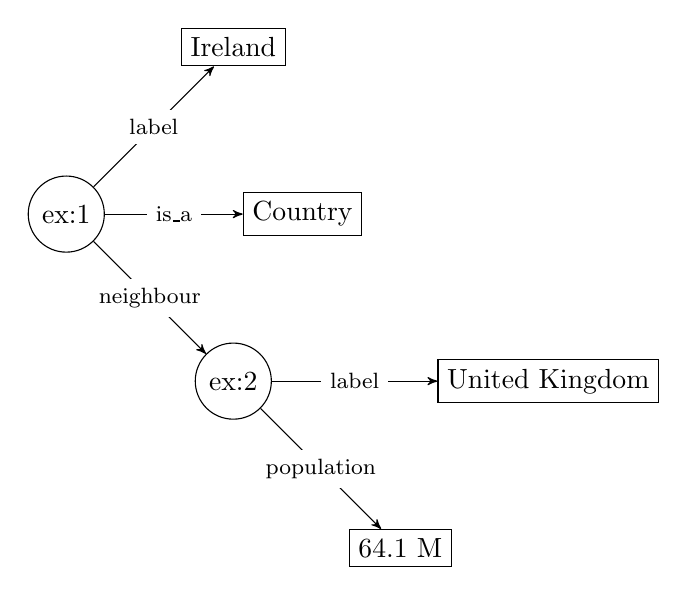
\begin{tikzpicture}[->,>=stealth',node distance=3cm]
\node[draw,circle] (a) {ex:1};
\node[draw,right of = a] (b) {Country};
\node[draw,above right of = a] (c) {Ireland};

\node[draw,circle,below right of = a] (d) {ex:2};
\node[draw,right of = d,xshift=1cm] (e) {United Kingdom};
\node[draw,below right of = d] (f) {64.1 M};

\path[every node/.style={fill=white,font=\footnotesize}]
(a) edge node {is\_a} (b)
(a) edge node {label} (c)
(a) edge node {neighbour} (d)
(d) edge node {label} (e)
(d) edge node {population} (f)
;
\end{tikzpicture}
		}
		\caption{A simple graph}
		\label{fig:bow-graph}
	\end{subfigure}
	\qquad
	\begin{subfigure}[b]{0.45\textwidth}
		\centering
		\resizebox{\textwidth}{!}{
			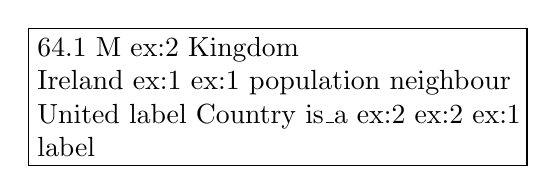
\begin{tikzpicture}
\node[draw,text width=6.1cm] {
64.1 M ex:2 Kingdom \newline
Ireland ex:1 ex:1
population neighbour United
label Country is\_a
ex:2 ex:2 ex:1 label
};
\end{tikzpicture}

		}
		\caption{Bag of words modelling}
		\label{fig:bow}
	\end{subfigure}
	\caption{A graph modelled as a bag of words}
\end{figure}

\section{Challenges}

A schema is the basis of many algorithms over the data. A schema describes the content thus facilitating users searching for a particular resource. A schema may provide statistical information about the data, which is useful for query optimisation. Schemas help in the integration process of several data sources. As a consequence, a major challenge is to determine what features of the data can be used in order to effectively generate a schema.

Applications may need different information about the data from the schema. Indeed, some errors in the schema can be acceptable for a user exploring the data, but not for a query optimizer. Hence, it is necessary to measure how accurate a schema is with regards to the data.

In the recent years, the amount of data has been growing increasingly. A glimpse of this growth over the years can be visually appreciated\footnote{The Linking Open Data cloud diagram: \url{http://lod-cloud.net/}} through the various diagrams. It is common to see data with millions of entities and billions of statements, to which the ``Open Data'' movement contributed a significant part. However, the ease of sharing data has the downside of that data not following a strict schema, if any. As a consequence, there is a need for techniques that can provide a schema without restraining the ``evolution'' of the data, while at the same time that can scale to large volumes of data.

\section{Scope of the Research}

The scope of this thesis is to study the extraction of schemas from large scale semi-structured information sources. By semi-structured we refer to data that present some structured but that is not followed strictly by all records in the data set. By large scale we mean data which contain millions of entities with billions of statements describing said entities.

The main challenge is to present a schema extraction process that is able to cope with the scale of the data, as well as with the variability of the data due to the heterogeneous and loose use of vocabularies. To this end, we investigate graph summarisation approaches which generate schemas via graph homomorphism. Due to the heterogeneity of the data, the generation of \emph{approximate} schemas is the only viable option.

Different applications have varying interactivity with respect to the schema. We investigate ranking techniques for retrieving first the parts of the schema an application need. We evaluate how ranking can be used for improving the exploration of data.

\section{Applications}

Graph summarisation produces a \emph{summary} of the graph's structure, providing information akin to a schema in relational databases. We can then leverage the summary in various ways, of which some are presented in this thesis.

\begin{labeling}{\emph{Browsing of a dataset's structure.}}
\item[\emph{Querying assistance.}] We use the structural information from a summary in order to assist a user in writing a query. This allows users having little to no knowledge about the data to build meaningful queries.

\item[\emph{Browsing of a dataset's structure.}] The information gathered during the graph summarisation process of a dataset is made available for browsing. This enables a user to learn about the internals of a dataset: its structure, the kind of information it carries, the relationships between concepts, or its connections to other datasets.
\end{labeling}

\section{Outline}

The thesis is divided in four parts. This first part \emph{Prelude} contains the introduction to the thesis. The second \emph{Foundations} presents fundamental concepts and models that will reused throughout the rest of the thesis. We introduce in the third part \emph{Methods} new techniques for generating and evaluating graph schemas, as well as a new ranking model for semi-structured data. In the final part \emph{Putting the Pieces Together}, we describe applications of the presented methods.

\minisec{Part II: Foundations}

\begin{labeling}{Chapter~\ref{chap:ssd}:}
\item[Chapter~\ref{chap:ssd}:] We present here a graph data model that encompasses the various formats used for modelling structured data. The model is layered so to represent the concepts of entity and dataset. Then we describe a graph schema model which fits between those two layers.
\end{labeling}

\minisec{Part III: Methods}

\begin{labeling}{Chapter~\ref{chap:summary}:}
\item[Chapter~\ref{chap:summary}:] We discuss current approaches at summarising graphs and the targeted use cases. We present a technique for generating graph schemas for Web Data at scale. Also, we introduce a model for measuring the quality of a generated graph schema.
\item[Chapter~\ref{chap:tree-ranking}:] In this chapter, we introduce a ranking model for semi-structured data. The model considers the structural heterogeneity of the data for a better scoring of entities.
\item[Chapter~\ref{chap:summary-ranking}:] We discuss in this chapter how the ranking model is applied on generated graph schemas. This allows to rank parts of a graph schema with regards to a graph-shaped query.
\end{labeling}

\minisec{Part IV: Putting the Pieces Together}

\begin{labeling}{Chapter~\ref{chap:system}:}
\item[Chapter~\ref{chap:system}:] In this chapter, we present applications of the introduced methods. We develop a system based on a generated schema that assists users in writing graph-shaped queries without a priori knowledge of the data structure. We develop an application that provides a structural description of datasets, as well as the connections between datasets. Finally, we make available a repository of generated graph schemas to the Web of Data community in order to facilitate the browsing and applications of Web Data.
\end{labeling}

\section{Contributions}

In this work, the main contribution is a method for generating schemas from large and distributed semi-structured datasets. We apply this methodology for providing a repository of generated schemas to foster applications on Web Data. To this end, we investigate the aspects of graph summarisation and semi-structured data ranking. Specific contributions include:

\begin{itemize}
\item a formal model for graph schema with varying granularity in Chapter~\ref{chap:ssd};
\item a method for generating graph schemas of large and distributed semi-structured data in Chapter~\ref{chap:summary};
\item a novel ranking model specifically design for dealing with the structural and content heterogeneity of Web Data in Chapter~\ref{chap:tree-ranking}; and
\item a set of tools for improving the exploitation of semi-structured data in Chapter~\ref{chap:system}.
\end{itemize}


%\part{Foundations}

\chapter{Semi-Structured Data}
\label{chap2:semi-structured-data}

Despite the fact that the Web is best known as a large collection of textual documents, it also provides an increasing amount of structured data sources in a wide range of formats, from HTML tables to Deep Web databases, XML documents, documents embedding semantic markups, e.g., Microformats, Microdata, RDF, RDFa. Structured data on the Web covers a large range of domains, e.g., e-commerce, e-government, social network, science, editorial world, \ldots, and can describe any kind of \emph{entities}, e.g., people, organisations, products, locations, etc. We face the challenge of handling the heterogeneity of the data representation.

In some areas, information is commonly represented with graphs, since it is expressive enough for modelling data with complex relationships. Graphs are used in social science for describing interactions between people. Graphs such as semantic networks~\cite{sowa2006semantic} have been used in artificial intelligence and machine translation, with the Semantic Web being a large scale instance.

Therefore, we base this thesis work on a graph data model in order to account for the variety of data.

%\subsection{Web Data}
%\label{chap2:semi-structured-data:gdm:wod}
%
%The \emph{Web Data} is a collection of structured data sources that are exposed on the Web through various forms such as HTML tables, Deep Web databases, XML documents, documents embedding semantic markups, e.g., Microformats, Microdata, RDF, RDFa. Since each data source might have its own defined schema, ranging from loosely to strictly defined, the data structure does not follow strict rules as in a database. Even within a given data source, the schema might not be fixed and may change as the information grows. The information structure evolves over time and new entities can require new attributes. We therefore consider the Web of Data as being \emph{semi-structured}~\cite{abiteboul:1997:icdt}. In this context, we consider a graph as a generic model for representing data.

\section{Semi-Structured Data Models}

Information on the Web is available in variety of formats and design, e.g., from HTML tables to documents embedding semantic markups. Each data source has its own schema, ranging from loosely to strictly defined. The data evolves over time, e.g., new attributes are required or new entities have been integrated from an external source. As such, data that does not follow a strict schema is called \emph{semi-structured}~\cite{abiteboul:1997:icdt}.

\minisec{OEM --- Object Exchange Model}

A seminal work in modelling semi-structured is the OEM model~\cite{papakonstantinou:1995:oea}. OEM served as the basic data model in projects such as Tsimmis~\cite{chawathe:1994:ipsj}, Lore~\cite{quass:1996:sigmod} and Lorel~\cite{abiteboul:97:ijdl}. In the Object Exchange Model, the data is a collection of objects, where each object can be either atomic or complex. An atomic object represents some base data types, while a complex object is a (attribute, object) pair. OEM is a graph-based data model, where the nodes are the objects and the edges are labelled with attribute names.

\minisec{XML --- Extensible Markup Language}

XML~\cite{bray:1998:xml} is a W3C standard for exchanging data on the Web. Nested, tagged elements are the building blocks of XML. A tagged element can have attribute value pairs and sub-elements. A sub-element may be either a tagged element or an atomic value such as text. XML is well suited for semi-structured data since there is no restriction regarding the naming of tags or the relationships between tags.

\minisec{RDF --- Resource Description Format}

RDF~\cite{klyne_carroll:2004} is a generic data model proposed for exchanging data on the Web. A resource description in RDF is composed of statements about the resource. A statement asserts that a resource has a value associated with a property. It is modelled as a triple consisting of a subject, a predicate, and an object. A set of RDF statements forms a directed labelled graph. While it is similar to the OEM model, RDF proposes some additional features such as the use of URIs as global identifiers which helps to avoid ambiguities and enables the creation of a global data graph.

Any kind of data can generally be modelled using a graph, since it is versatile enough to accommodate different specifications. As such, we build the work in this thesis upon a generic graph model.

\section{Abstract Model}
\label{chap2:semi-structured-data:gdm:abstract-model}

We consider the data as being a labelled directed graph and build methods based on this model. Therefore, the findings presented in this work can be applied to any domain where a graph is used as data representation.

We describe in this Section a graph data model based on the work of \cite{delbru:jws:entity}. The graph is represented with two layers that depict the data at two extremes: the \emph{dataset} and the \emph{entity} layers. We formally introduce the concepts of entity and dataset in Sections~\ref{chap2:semi-structured-data:entity-description} and~\ref{sec:ssd:dataset}, respectively. The Figure~\ref{chap2:semi-structured-data:fig:gdm} depicts the layers of the model, where the dataset layer is depicted at the top, and the entity layer at the bottom.
\begin{labeling}{\textbf{Dataset Layer:}}
	\item[\textbf{Dataset Layer:}] A dataset represents a collection of entities; the dataset layer is the ensemble of entities' collections. This layer provides coarse information about the data: the focus of this layer is the relationships between datasets. In the figure, the dataset \emph{D1} connects to the dataset \emph{D2} via the link \emph{p1}, and \emph{D2} is connected to \emph{D1} via two links, i.e., \emph{p2} and \emph{p3}.
	\item[\textbf{Entity Layer:}] The entity layer contains information about entities. Of the two layers, this one provides the finer details about the data: attributes about an entity, and also relationships between entities. In the figure, the entity layer provides additional information about the dataset layer, showing which entities are actually connected within --- and between --- datasets.
\end{labeling}

The dataset layer shows the links between datasets, i.e., \emph{inter-dataset} links, while the entity layer provides in addition information on the links within a dataset, i.e., \emph{intra-dataset} links.

The dataset layer is blind to the information the entity layer provides: its focus is on the relationships between datasets, and not between the entities that compose the datasets.

Regardless of the layer, we represent the information using a node and edge labelled directed graph, referred simply as a \emph{graph} from this point on. Also, we will call the graph on the dataset layer the \emph{dataset graph}, and the graph on the entity layer the \emph{entity graph}.

\begin{figure}
	\centering
	\resizebox{.8\textwidth}{!}{
		\input{02-foundations/figures/graph-abstract-model}
	}
	\caption{The graph data abstract model}
	\label{chap2:semi-structured-data:fig:gdm}
\end{figure}

\section{Formal Model}
\label{chap2:semi-structured-data:gdm:formal-model}

In the following we formally define a directed labelled graph that we call simply a graph henceforth, and introduce concepts used in the rest of the thesis. We use a graph as a generic representation of (semi-)structured and unstructured data on the Web of Data. A graph is defined as a tuple consisting of a set of nodes $V$ and a set $A$ of directed edges labelled $a$. We consider edge and node labels to come from a set that we denote with $\mathcal{L}$. Figure~\ref{chap2:semi-structured-data:fig:graph} depicts a graph of people and places along with their connections.

\begin{definition}[Graph]
	Let $V$ be a set of nodes and $\mathcal{L}$ a set of labels. The set of directed labelled edges is defined as $A \subseteq \left\lbrace (x, \alpha, y) \mid (x, y) \in V^2, \alpha \in \mathcal{L} \right\rbrace$.

	A \emph{graph} $G$ is a tuple $G = \left\langle V, A, l_V \right\rangle$ where $l_V : V \mapsto \mathcal{L}$ is a node-labelling function.
\end{definition}

Given a graph $G = \left\langle V, A, l_V \right\rangle$, we introduce below terms used throughout the thesis.

\begin{labeling}{\textbf{Attribute}}
	\item[\textbf{Edge}] An edge labelled $\alpha$ from the node $x$ to the node $y$ is written as $\left(x, \alpha, y\right)$. We say that $x$ is the \emph{source}, and $y$ is the \emph{target}.

	\item[\textbf{Path}] We call a \emph{path} a sequence of edges label $\alpha_1.\cdots.\alpha_n$. A path exists in the graph $G$ if there is a sequence of nodes $\left\lbrace v_1, \cdots, v_{n+1} \right\rbrace \subseteq V$ connected with such labelled edges.

	In Figure~\ref{chap2:semi-structured-data:fig:graph} the path $author.lives$ exists in that graph as it connects the nodes $\left\lbrace v_0, v_2, v_3 \right\rbrace$.

	\item[\textbf{Attribute}] We call \gls{edge-attribute} the label of an edge.

		We define as $\gls{attributes}\left(x \in V\right) = \left\lbrace \alpha \in \mathcal{L} \mid \exists y \in V, (x, \alpha, y) \in A \right\rbrace$ the set of attributes associated as a source with a node $x$ in $G$. In the figure, we have $attributes(v_1) = \{lives,works,name,\tau\}$.

		Similarly, we define the set of \gls{incoming-attributes} as
	$$
	attributes^{-1}\left(x \in V\right) = \left\lbrace \alpha \in \mathcal{L} \mid \exists w \in V, (w, \alpha, x) \in A \right\rbrace
	$$
	\item[\textbf{Value}] We call \emph{value} the label of a node which is the target of an edge.

	\item[\textbf{$k$-hop}] We say that two nodes are $k$-hop away if there is a path composed of $k$ edges label connecting the two. For example in the figure, the nodes $v_1$ and $v_6$ are 2-hops away because of the path $lives, location$.

	\item[\textbf{Size}] The size of a graph is defined as the number of edges $\vert A \vert$ that the graph is composed of.
\end{labeling}

\begin{figure}
	\centering
	\resizebox{\textwidth}{!}{
		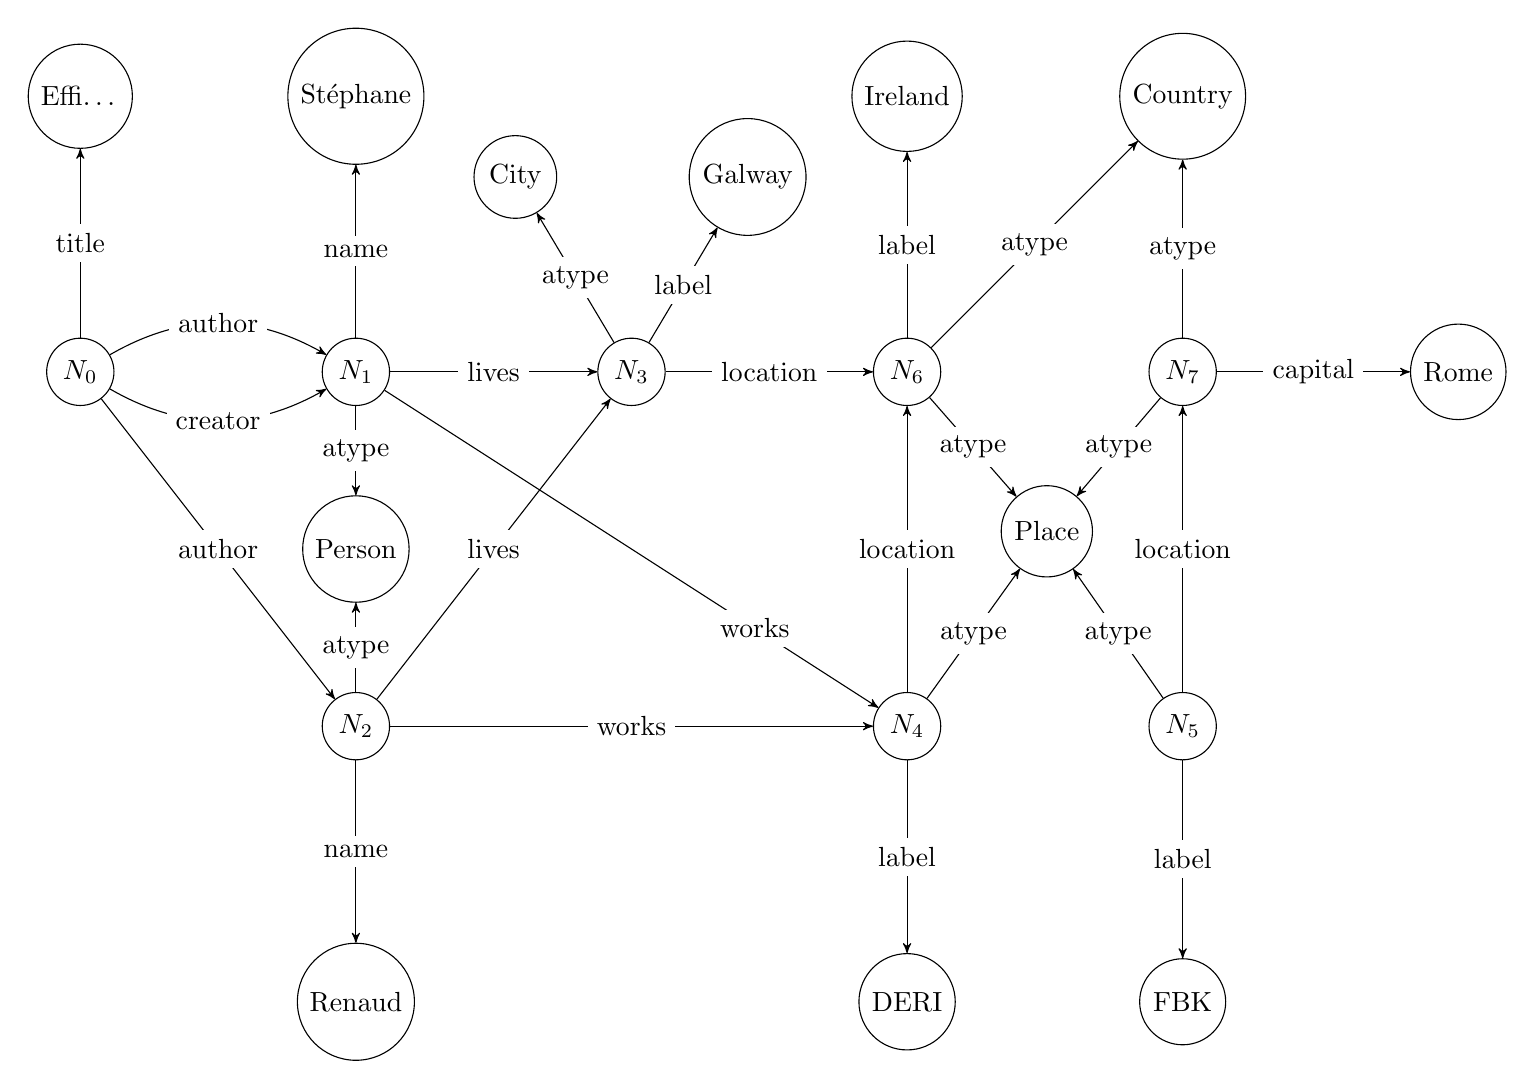
\begin{tikzpicture}[->,>=stealth',node distance=3.5cm]
\node [draw,circle] (n0) {$N_0$};
\node [draw,circle,above of = n0] (effi) {Effi\ldots};
\node [draw,circle,right of = n0] (n2) {$N_1$};
\node [draw,circle,below of = n2,yshift=-1cm] (n1) {$N_2$};
\node [draw,circle,right of = n2] (n3) {$N_3$};
\node [draw,circle,right of = n3] (n6) {$N_6$};
\node [draw,circle,below of = n6,yshift=-1cm] (n4) {$N_4$};
\node [draw,circle,below of = n2,yshift=1.25cm] (person) {Person};
\node [draw,circle,below of = n1] (ren) {Renaud};
\node [draw,circle,above of = n2] (ste) {St\'ephane};
\node [draw,circle,right of = n4] (n5) {$N_5$};
\node [draw,circle,right of = n6] (n7) {$N_7$};
\node [draw,circle,above right of = n4,xshift=-.7cm] (place) {Place};
\node [draw,circle,above of = n7,yshift=0cm] (country) {Country};
\node [draw,circle,below of = n4] (deri) {DERI};
\node [draw,circle,below of = n5] (fbk) {FBK};
\node [draw,circle,above left of = n3,xshift=1cm] (city) {City};
\node [draw,circle,above right of = n3,xshift=-1cm] (gal) {Galway};
\node [draw,circle,right of = n7] (rome) {Rome};
\node [draw,circle,above of = n6] (ire) {Ireland};

\path
(n7) edge node[fill=white] {capital} (rome)
(n6) edge node[fill=white] {label} (ire)

(n3) edge node[fill=white] {label} (gal)
(n3) edge node[fill=white] {\glssymbol{atype}} (city)

(n4) edge node[fill=white] {label} (deri)
(n5) edge node[fill=white] {label} (fbk)

(n6) edge node[fill=white] {\glssymbol{atype}} (country)
(n7) edge node[fill=white] {\glssymbol{atype}} (country)

(n4) edge node[fill=white] {\glssymbol{atype}} (place)
(n5) edge node[fill=white] {\glssymbol{atype}} (place)
(n6) edge node[fill=white] {\glssymbol{atype}} (place)
(n7) edge node[fill=white] {\glssymbol{atype}} (place)

(n3) edge node[fill=white] {location} (n6)
(n4) edge node[fill=white] {location} (n6)
(n5) edge node[fill=white] {location} (n7)
(n1) edge node[fill=white] {name} (ren)
(n2) edge node[fill=white] {name} (ste)
(n1) edge node[fill=white] {\glssymbol{atype}} (person)
(n2) edge node[fill=white] {\glssymbol{atype}} (person)
(n0) edge node[fill=white] {title} (effi)
(n0) edge[bend right] node[fill=white] {creator} (n2)
(n0) edge[bend left] node[fill=white] {author} (n2)
(n0) edge node[fill=white] {author} (n1)
(n1) edge node[fill=white] {lives} (n3)
(n1) edge node[fill=white] {works} (n4)
(n2) edge node[fill=white] {lives} (n3)
(n2) edge[near end] node[fill=white] {works} (n4)
;
\end{tikzpicture}

%\begin{tikzpicture}[scale=2.75,>=triangle 45]
%\GraphInit[vstyle=Normal]
%%\draw[help lines] (0,-2) grid (7,2);
%
%% doc
%%\SetVertexNormal[LineColor=red]
%\Vertex[Math,x=0,y=.75]{N_0}
%%\SetVertexNormal[LineColor=black]
%\Vertex[x=0,y=1.75,L=Effi...]{doc}
%\Edge[style={->},label=title](N_0)(doc)
%% Person
%%\SetVertexNormal[LineColor=red]
%\Vertex[Math,x=1.75,y=-.75]{N_1}
%\Vertex[Math,x=1.75,y=.75]{N_2}
%%\SetVertexNormal[LineColor=black]
%\Vertex[x=.6,y=.2]{Person}
%\Vertex[x=1,y=1.75,L=St\'ephane]{ste}
%\Vertex[x=.25,y=-1,L=Renaud]{ren}
%\Edge[style={->},label=type](N_1)(Person)
%\Edge[style={->},label=type](N_2)(Person)
%\Edge[style={->},label=name](N_2)(ste)
%\Edge[style={->},label=name](N_1)(ren)
%\Edge[style={->},label=creator](N_0)(N_2)
%\Edge[style={->,bend left},label=author](N_0)(N_2)
%\Edge[style={->,bend right=40},label=author](N_0)(N_1)
%% City
%%\SetVertexNormal[LineColor=red]
%\Vertex[Math,x=3,y=.78]{N_3}
%%\SetVertexNormal[LineColor=black]
%\Vertex[x=2,y=1.5]{City}
%\Vertex[x=3,y=1.75]{Galway}
%\Edge[style={->},label=type](N_3)(City)
%\Edge[style={->,bend right},label=label](N_3)(Galway)
%\Edge[style={->,bend left},label=lives](N_1)(N_3)
%\Edge[style={->},label=lives](N_2)(N_3)
%%% Organisation
%%\SetVertexNormal[LineColor=red]
%\Vertex[Math,x=3,y=-.75]{N_4}
%\Vertex[Math,x=3,y=-1.25]{N_5}
%%\SetVertexNormal[LineColor=black]
%\Vertex[x=4.5,y=-.75]{Place}
%\Vertex[x=3,y=.19]{DERI}
%\Vertex[x=1.75,y=-1.3]{FBK}
%\Edge[style={->},label=type](N_4)(Place)
%\Edge[style={->},label=type](N_5)(Place)
%\Edge[style={->},label=label](N_5)(FBK)
%\Edge[style={->},label=label](N_4)(DERI)
%\Edge[style={->},label=works](N_1)(N_4)
%\Edge[style={->,bend right},label=works](N_2)(N_4)
%% Country
%%\SetVertexNormal[LineColor=red]
%\Vertex[Math,x=4.5,y=.25]{N_6}
%\Vertex[Math,x=5.75,y=-.8]{N_7}
%%\SetVertexNormal[LineColor=black]
%\Vertex[x=5.5,y=1.5]{Country}
%\Vertex[x=4,y=1.5]{Ireland}
%\Vertex[x=5.2,y=0.2]{Rome}
%\Edge[style={->},label=type](N_6)(Country)
%\Edge[style={->,bend right=20},label=type](N_7)(Country)
%\Edge[style={->},label=type](N_6)(Place)
%\Edge[style={->},label=type](N_7)(Place)
%\Edge[style={->},label=label](N_6)(Ireland)
%\Edge[style={->},label=capital](N_7)(Rome)
%\Edge[style={->},label=location](N_4)(N_6)
%\Edge[style={->},label=location](N_3)(N_6)
%\Edge[style={->,bend right=20},label=location](N_5)(N_7)
%\end{tikzpicture}

%\begin{tikzpicture}[>=triangle 45]
%
%\begin{dot2tex}[dot,tikz,codeonly,options=--tikzedgelabels -c]
%
%digraph G {
%	node [shape="circle"];
%
%	n0 [texlbl="$N_0$"];
%	n1 [texlbl="$N_1$"];
%	n2 [texlbl="$N_2$"];
%	n3 [texlbl="$N_3$"];
%	n4 [texlbl="$N_4$"];
%	n5 [texlbl="$N_5$"];
%	n6 [texlbl="$N_6$"];
%	n7 [texlbl="$N_7$"];
%
%	eff [label="Effi..."];
%	ste [texlbl="St\'ephane"];
%	ren [texlbl="Renaud"];
%	Person [label="Person"];
%	City [label="City"];
%	fbk [label="FBK"];
%	deri [label="DERI"];
%	galway [label="Galway"];
%	Place [label="Place"];
%	Country [label="Country"];
%	ireland [label="Ireland"];
%	rome [label="Rome"];
%
%	edge [lblstyle="fill=white"];
%
%	n0 -> eff [label="title"];
%	n0 -> n2 [topath="bend right",label="author"];
%	n0 -> n2 [topath="bend left",label="creator"];
%	n0 -> n1 [label="author"];
%
%	n1 -> Person [label="type"];
%	n1 -> ren [label="name"];
%	n1 -> n4 [label="works"];
%	n1 -> n3 [label="lives"];
%
%	n2 -> Person [label="type"];
%	n2 -> ste [label="name"];
%	n2 -> n3 [label="lives"];
%	n2 -> n4 [label="works"];
%
%	n3 -> City [label="type"];
%	n3 -> galway [label="label"];
%	n3 -> n6 [label="location"];
%
%	n4 -> deri [label="label"];
%	n4 -> n6 [label="location"];
%	n4 -> Place [label="type"];
%
%	n5 -> fbk [label="label"];
%	n5 -> Place [label="type"];
%	n5 -> n7 [label="location"];
%
%	n6 -> Country [label="type"];
%	n6 -> ireland [label="label"];
%	n6 -> Place [label="type"];
%
%	n7 -> Place [label="type"];
%	n7 -> Country [label="type"];
%	n7 -> rome [label="capital"];
%}
%
%\end{dot2tex}
%
%\end{tikzpicture}
	}
	\caption{An entity graph describing people, places, and their relationships.}
	\label{chap2:semi-structured-data:fig:graph}
\end{figure}

\subsection{Type Attribute}
\label{sec:ssd:type}

Attributes and node labels can be used in a graph for describing the content. For example in Figure~\ref{chap2:semi-structured-data:fig:graph}, we can expect that the value of the edge labelled ``name'' represents a textual identification of the node $v_1$. In addition, a set of nodes may represent a same concept, e.g., the nodes $v_1$ and $v_2$ represent a person. We call, e.g., ``person'', the \emph{type} of a node, and that node is an \emph{instance} of that type.

We model this in a graph thanks to an edge where
\begin{inparaenum}[(1)]
\item the source is an instance;
\item the target is the type; and
\item the attribute is a certain pre-defined label that we denote as $\tau$.
\end{inparaenum}
That certain attribute is used to indicate that the target of the edge represents a type; in RDF, it is commonly the \emph{rdf:type}\footnote{RDF type attribute: \url{http://www.w3.org/1999/02/22-rdf-syntax-ns\#type}} attribute.

Since there may be several attributes that can hold this function, we refer to them as the \emph{type attributes}. For example in Figure~\ref{chap2:semi-structured-data:fig:graph}, the edge $(v_1, \tau, \text{Person})$ indicates that the node $v_1$ is an instance of type \emph{Person}.
We define $T$ as the set of \emph{type attributes}, and we denote an element of that set with $\tau$.%, in order to abstract from the actual type attribute used.

\begin{definition}[Type Attributes Set $T$]
Let $T \subset \mathcal{L}$ be a subset of labels.
We define $T$ as the set of type attributes, and we call $\glssymbol{atype} \in T$ a type attribute.
\end{definition}

For a given node $x \in V$, we consider $\gls{types}(x)$ as the set of values for which the attribute is a type attribute.

$$
types(x\in V) = \left\lbrace l_V(c) \mid \exists c \in V\; \exists \glssymbol{atype} \in T: (x, \glssymbol{atype}, c) \in A \right\rbrace
$$

For instance, we have $types\left(v_6\right) = \left\{ \text{Country}, \text{Place} \right\}$ in Figure~\ref{chap2:semi-structured-data:fig:graph} as the set of type values for the node $v_6$.

\subsection{Entity description}
\label{chap2:semi-structured-data:entity-description}

The Web Data represents a graph of interconnected \emph{entities}, where an entity may be a person, a place, or an organisation, \ldots. We call an \emph{entity description} the pieces of informations in the graph that are about that entity. For instance, we can consider ``Galway'' to be part of the entity description of $v_3$ in Figure~\ref{chap2:semi-structured-data:fig:graph}, but not ``Rome''.

There exists several ways to define which parts of the graph describe an entity. One may consider all the edges, incoming and outgoing, to form the entity description. For some graphs, edges that are two-hops away might be part of it too.

We illustrate this in Figure~\ref{chap2:semi-structured-data:fig:edesc} where we might consider the entity description to consist of edges 1-hop away from the node given the graph in Figure~\ref{chap2:semi-structured-data:fig:edesc1}, although it is more adapted to extend it to 2-hops with the graph in Figure~\ref{chap2:semi-structured-data:fig:edesc2}. The reason for the design in the latter graph might be to add more information about a person's label, e.g., the honorific.

\begin{figure}
	\centering
	\begin{subfigure}[b]{.45\textwidth}
		\resizebox{.6\textwidth}{!}{
			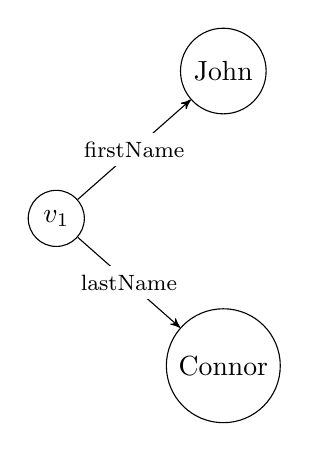
\begin{tikzpicture}[->,>=stealth',node distance=3cm]
\node[draw, circle] (a) {$v_1$};
\node[draw, circle, above right of = a,yshift=-.25cm] (b) {John};
\node[draw, circle, below right of = a,yshift=.25cm] (c) {Connor};

\path[every node/.style={font=\footnotesize}]
(a) edge node[fill=white] {firstName} (b)
(a) edge node[fill=white] {lastName} (c)
;
\end{tikzpicture}
		}
		\caption{1-hop entity description}
		\label{chap2:semi-structured-data:fig:edesc1}
	\end{subfigure}
	\quad
	\begin{subfigure}[b]{.45\textwidth}
		\resizebox{\textwidth}{!}{
			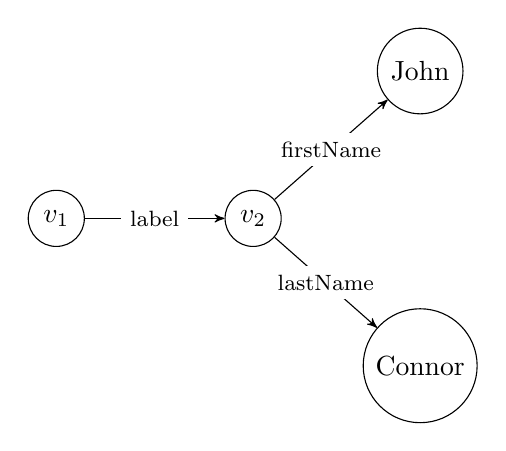
\begin{tikzpicture}[->,>=stealth',node distance=3cm]
\node[draw, circle] (a) {$v_1$};
\node[draw, circle,right of = a,xshift=-.5cm] (aa) {$v_2$};
\node[draw, circle, above right of = aa,yshift=-.25cm] (b) {John};
\node[draw, circle, below right of = aa,yshift=.25cm] (c) {Connor};

\path[every node/.style={font=\footnotesize}]
(a) edge node[fill=white] {label} (aa)
(aa) edge node[fill=white] {firstName} (b)
(aa) edge node[fill=white] {lastName} (c)
;
\end{tikzpicture}
		}
		\caption{2-hops entity description}
		\label{chap2:semi-structured-data:fig:edesc2}
	\end{subfigure}
	\caption{Interpretation of the entity description dependent on the graph structure.}
	\label{chap2:semi-structured-data:fig:edesc}
\end{figure}

%In this thesis, we do not attempt to find the most appropriate entity description for a given graph. We choose the approach taken in Delbru et. al.~\cite{delbru:jws:entity}, where an entity description consists of the \emph{outgoing} edges adjacent to a node. This forms then what we call a \emph{star graph}.
%
%\begin{definition}[Entity Description]
%Let $G = \left\langle V, A, l_V \right\rangle$ be a graph. We define the \emph{entity description} $\glssymbol{edesc}(u \in V)$ as the set of outgoing edges:
%$$
%\glssymbol{edesc}(u \in V) = \left\lbrace (u, \alpha, v) \in A \mid \exists v \in V \right\rbrace
%$$
%\end{definition}

\begin{definition}[Entity Description]
Let $G = \left\langle V, A, l_V \right\rangle$ be a graph. We define the entity description of a node $u \in V$ as the set of edges $\glssymbol{edesc}(u) \subseteq A$ that describe that node.
\label{chap2:semi-structured-data:def:entity-description}
\end{definition}

For example, if we consider the outgoing edges to form the entity description, we have for the node $v_6$ the following set:
$$
\begin{aligned}
\mathcal{E}\left( v_6 \right) = \{ & \left( v_6, \text{label}, \text{Ireland} \right),\\
& \left( v_6, \tau, \text{Country} \right),\\
& \left( v_6, \tau, \text{Place} \right) \}
\end{aligned}
$$

\subsection{Dataset}
\label{sec:ssd:dataset}

In the Web of Data, a dataset~\cite{alexander:2009:dld} represents a collection of \emph{edges} which, e.g., are located in a same website, or share a common topic. A dataset can be a \emph{dump} in RDF, or the embedded metadata of pages in a website.
%A dataset can refer to graphs from a collection of sources, e.g., several websites.
%	In the Web Data scenario, we identify a dataset label by the top-level domain (TLD) name of an  's URI as in Delbru~\cite{delbru:jws:entity}. In RDF, we determine the dataset label of a statement based on the TLD of the subject's resource. If the latter is a \emph{blank node}, the website that hosts the data is then considered as the dataset. For instance, the statement below belongs to the dataset \emph{dbpedia.org}.
%	\begin{quote}
%		{\small $<$\url{http://dbpedia.org/resource/Tim_Berners-Lee}$>$ rdf:type foaf:Person .}
%	\end{quote}

\begin{definition}[Dataset]
Let $G_1, \cdots, G_i, \cdots, G_n$ be $n$ graphs such that $G_i = \left\langle V_i, A_i, l_{V_i} \right\rangle$ is a graph.
Let $\glssymbol{Glabel} : G \mapsto \mathcal{L}$ be a function that assigns a label to a graph.
We define a dataset as the tuple $\left\langle D, \alpha \right\rangle$, where $D = \left\lbrace G_1, \cdots, G_n \right\rbrace$ and $\alpha \in \mathcal{L}$ is the dataset label such that $\forall 0 < i \le n\; \glssymbol{Glabel}(G_i) = \alpha$.
\end{definition}

We extend without loss of generality the definitions presented in this chapter to a dataset, which we indicate by adding a subscript $d$. We shall omit this subscript if it is clear from the context that only one dataset is considered. Therefore, we have the following definitions:

\begin{itemize}
\item $G_d = \left\langle V_i, A_i, l_{V_i} \right\rangle$: The label of the graph $G$ is $d$, i.e., $l_G(G) = d$.
\item $\glssymbol{edesc}_d$: The edges from the entity description belong to a graph which dataset label is $d$.
\end{itemize}


\chapter{Ranking of (Semi-)Structured Data}

At its beginning, The Internet was a collection of hypertext documents: textual data with links to additional textual data. At first, search engines were focused on retrieving documents, but with the growth of The Internet, a need for \emph{ranking} documents with regards to how important they are regarding a user's query appeared. Documents consisting only of text, the ranking models assumed as much and no structural information was considered. Nonetheless, some structural cues could still be extracted from the documents, e.g., title, paragraphs, links, \ldots, thanks to the HTML markup are written in. Including these cues into the ranking model improved noticeably its performance.

With the coming of the Semantic Web, documents are turning into a real blend of structured and unstructured data. The structural information is clearly defined. Since this marked a shift of how documents are modelled, there was a need for ranking models to adapt. In this chapter, we present some ranking models used over (semi-)structured data, and introduce the ranking model used in this thesis as a basis for Chapter~\ref{chap:tree-ranking}.

\section{Traditional Ranking Models}

\section{Abstract Model}

\section{Formal Model}

%\section{Entity Model}
%\label{chap:entity-ranking:entity-model}
%
%In this section, we define what is an entity, i.e., the unit of information that is queried and retrieved by an IR search engine. The entity model is based on the graph model presented in Section~\ref{sec:gdm:formal-model}.% In this chapter, we use \emph{document} as an equivalent term for \emph{entity}, since a document is the common term for the object that is ranked in an IR search engine.
%
%An entity in a graph data model is defined as a sub-graph in which a node is considered as the \emph{root}. In RDF the root is the URI that represents that entity, e.g., the URI \url{http://dbpedia.org/page/Earth} for referring to the planet Earth. The edges related to that root form then what we call an \emph{entity}.
%
%\begin{definition}[Entity]
%Let $G = \left\langle V, A, l_V \right\rangle$ be a graph. We call an entity rooted in $u \in V$ a sub-graph of $G$ in which the edges and nodes are a related to the root $u$.
%\end{definition}
%
%There exist several ways to define which edges are related to a root node. We can consider the entity as the connected component that emerges from that root. This can be achieved by performing a breadth-first search starting at the root, and adding the traversed edges and nodes to the entity. Also, one may consider a set of unconnected sub-graphs as the entity according to a similarity measure.
%
%In this chapter, we use the approach described in~\cite{delbru:jws:entity}, where an entity is a star graph, i.e., a sub-graph with a node (the root) and its direct neighbouring nodes it links to. The Figure~\ref{fig:rdf-graph} displays how a graph can be split into four entities \emph{me}, \emph{\_:b1}, \emph{\_:b2} and \emph{paper/547}. Each entity forms a sub-graph containing the incoming and outgoing edges of the root node. In order to simplify the extraction process, we only consider the outgoing edges of a root node.

%\subsubsection{Entity Model}
%
%In the remainder of the paper, the unit of information which is retrieved and ranked is an \emph{entity}~\cite{delbru:jws:entity} and is formalised as a list of attribute-value pairs:
%\begin{description}
%  \item[Entity] represents a set of attribute-value pairs and is identified by the entity node label, e.g., \emph{paper/547};
%  \item[Attribute] is an edge linking the entity node to one of its neighbour nodes and is identified by the edge label, e.g., \emph{title}, \emph{name} or \emph{creator};
%  \item[Value] is a neighbour node of the entity node and is identified by the node label, e.g., \emph{Object-} or \emph{paper/547}. A value is always associated to one attribute. Multiple values can be associated to a same attribute, such as the nodes \emph{\_:b1} and \emph{\_:b2} with the attribute \emph{knows} of the entity \emph{me}.
%\end{description}

\begin{figure}
\centering
\resizebox{0.65\textwidth}{!}{
    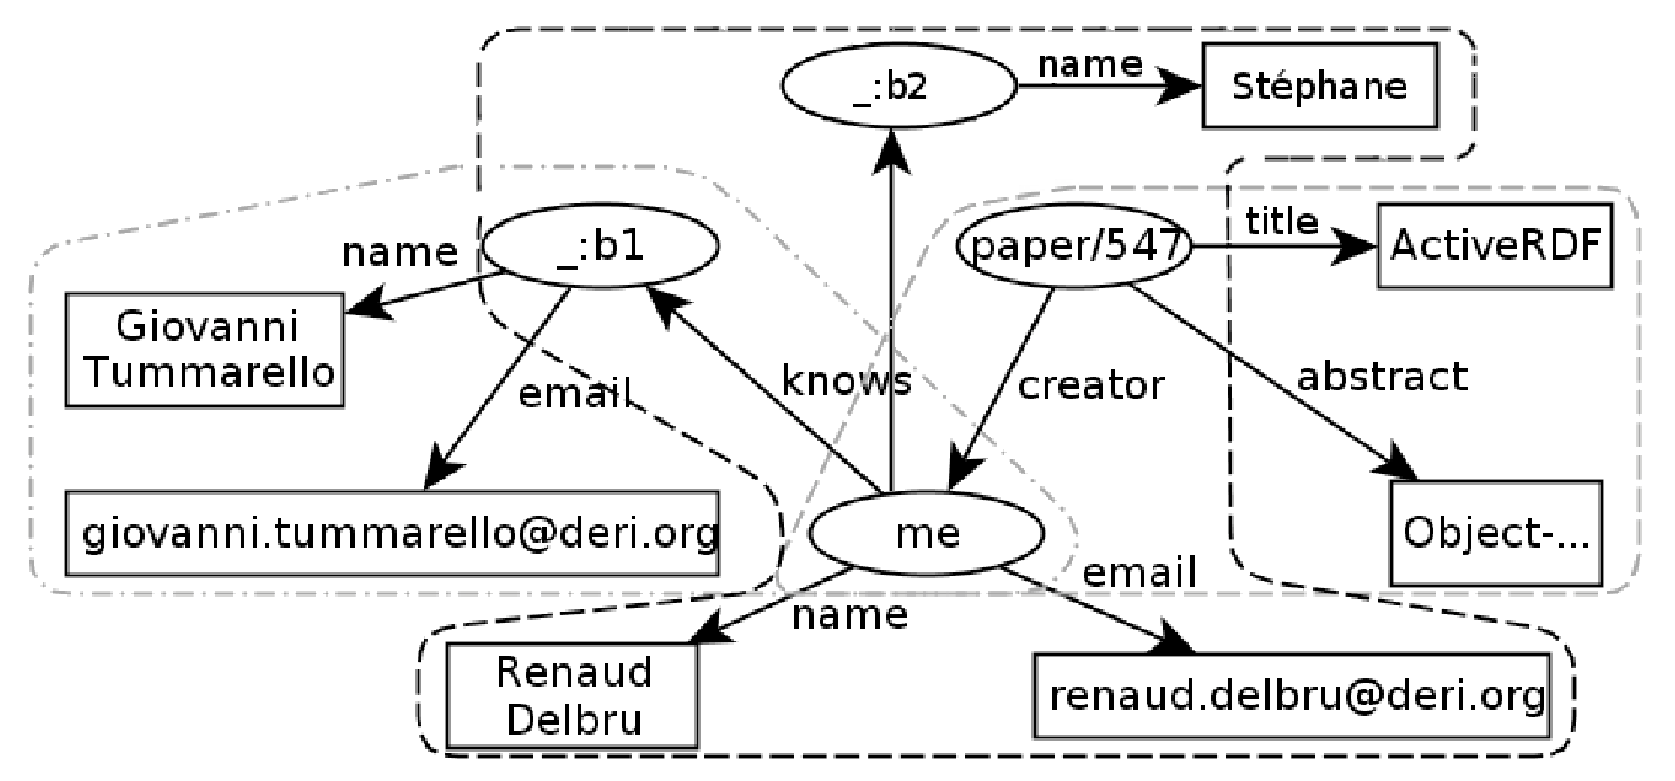
\includegraphics[scale=1]{05-ranking/figures/rdf-graph}
}
\caption{A graph divided into four entities identified by the root nodes \emph{me}, \emph{\_:b1}, \emph{\_:b2} and \emph{paper/547}.}
\label{fig:rdf-graph}
\end{figure}

\subsection{Field-Based Ranking Models}
\label{sec:ranking-wod}

In this section, we explain how to adapt two existing field-based ranking frameworks to the entity model.
A field-based ranking model views a document as composed of multiple normalized weighted fields. For example, a field can be the title, the author or the body of the document.

In the Probabilistic Relevance Framework\cite{Robertson:2009:PRF} (PRF), BM25F~\cite{zaragoza:2004:microsoft} is a popular web-search field-based ranking function.
The Divergence From Randomness\cite{amati:2002:acm} (DFR) framework gives birth to many ranking models, in particular to PL2F~\cite{macdonald:2005:clef} which is of the field-based family.

The mapping from the field-based document model to the entity model is straightforward. An entity can be seen as a document and all the edges with a same attribute as a document field. In presence of a multi-valued attribute, the common approach is to merge the content of all the values into one single value, i.e., creating a single bag of words.

\paragraph{Ranking features.}

The following features are used in the field-based ranking functions:
\begin{labeling}{\textbf{average field length}}
	\item[\textbf{field length}] refers to the number of terms in a value node label. In case of a multi-valued attribute, it refers to the number of terms across all the values associated to the attribute.
	\item[\textbf{average field length}] is equal to the mean of \emph{field length} across entities.
\end{labeling}

\paragraph{Normalised term frequency.}

The ranking models presented here are from the \emph{TF-IDF} family, where \emph{TF} is a function of the term frequency, and \emph{IDF} is a function of inverse document frequency. The intuition behind TF is that it captures the relevancy of a term within a document, e.g., the more a term occurs in a document, the more important it is for that document. In contrary, the intuition behind IDF is to capture the importance of a term within the collection of documents: the more a term occur in the collection, the less relevant it is. For example, the term ``food'' would occur frequently in a cooking recipes book, however it may not be an interesting feature in a ranking function.

In general, the term frequency is not used ``as is'' in the TF function, it is first \emph{normalised} before applying the TF function. Term frequency normalisation is useful in cases where the length of a document varies across the collection: it allows to capture this variability into the ranking function, making the score of documents comparable. In field-based ranking functions, the term frequency is normalized at the field level, capturing the length variability of a field across documents.

\subsubsection{BM25F Ranking Function}

Using BM25F, an entity $e$ is scored with regard to a query $q$ as follows:
\begin{eqnarray}
Score(e,q) & = & \alpha_e\times\sum_{t\in q}{q_t\times tfn \times \omega_t}\\
\label{eq:tfidf-score}
tfn & = & \frac{f_{t,e}\times(k_1+1)}{f_{t,e}+k_1} \\
\label{eq:bm25f_2}
f_{t,e} & = &
\sum_{a\in e}{\frac{\alpha_a\times f_{t,e,a}}{1+b_a\times\left(\frac{l_{e,a}}{l_a}-1\right)}}
\label{eq:bm25f_1}
\end{eqnarray}
in which the following notations are used:
\begin{itemize}
	\item $q_t$ is the weight of the query $q$ for the term $t$, i.e., its frequency within the query $q$;
	\item $tfn$ is the term frequency normalization function;
	\item $\omega_t$ is the IDF function of the term $t$;
	\item $k_1$ is the saturation parameter;
	\item $f_{t,e,a}$ is the frequency of the term $t$ in the attribute $a$ of the entity $e$;
	\item $\alpha_a$ is a weight of the attribute $a$ and $\alpha_e$ a weight of the entity $e$;
	\item $b_a$ is the normalization parameter for the attribute $a$ with $b_a \in \left[0,1\right]$;
	\item $l_{e,a}$ is the \emph{field length} of the attribute $a$ in the entity $e$; and
	\item $l_a$ is the \emph{average field length} of the attribute $a$.
\end{itemize}

The IDF function is defined as
$$
\omega_t=1+log\left(\frac{N}{N_t+1}\right)
$$
where $N$ is the total number of entities in the collection and $N_t$ is the total number of entities that have occurrences of the term $t$.

\subsubsection{PL2F Ranking Function}

DFR ranking models are based on the combination of three components, i.e., the information gain, the randomness model and the term frequency normalization model. PL2F bases the information gain on the Laplace after-effect model, uses Poisson as the model for randomness, and the \emph{normalization 2F} for the term frequency normalization.

Using PL2F, an entity $e$ is scored with regard to a query $q$ as follows:
\begin{eqnarray*}
	Score(e,q) & = & \alpha_e\times\sum_{t\in q}{qtw \times w_{e,t}}\\
	\label{eq:dfr-score}
	w_{e,t} & = & \left(1-P_{risk}\right) \times \left(-log_2\left(P_{P}\right)\right) \\
	\label{eq:dfr-term-weight}
	P_{risk} & = & \frac{tfn}{1+tfn} \\
	\label{eq:dfr-prisk}
	P_{P} & = & \frac{\lambda^{tfn}}{tfn!}\times e^{-\lambda} \:\text{ where }\: \lambda=\frac{F}{N} \\
	\label{eq:dfr:rand-poisson}
\end{eqnarray*}
in which the following notations are used:
\begin{itemize}
	\item $qtw=\frac{q_t}{q_{t,max}}$ is the weight of the query $q$ for the term $t$ with $q_{t,max}$ the maximum of $q_t$ in $q$;
	\item $w_{e,t}$ is the weight of the term $t$ in the entity $e$;
	\item $1-P_{risk}$ estimates the information gain of a term $t$;
	\item $-log_2\left(P_{P}\right)$ evaluates the importance of a term $t$ in the entity $e$ thanks to the Poisson model; and
	\item $F$ is equal to the frequency of the term $t$ in the collection.
\end{itemize}

The factorial is approximated with the Stirling's formula:
$$
tfn!=\sqrt{2\pi}\times tfn^{tfn+0.5}\times e^{-tfn}
$$

The term frequency of the term $t$ in the entity $e$ is normalized as follows:
\begin{equation}
tfn = \sum_{a\in e}{\alpha_a\times f_{t,e,a} \times log_2\left(1+c_a\times\frac{l_a}{l_{e,a}}\right)}
\label{eq:pl2f}
\end{equation}
where $c_a$ is a per-attribute hyperparameter with $c_a \in\;]0,+\infty[$.


%\chapter{Graph Summarisation}
\label{chap:summary}

In many Computer Science areas, the information is represented as and is analysed through graphs. Graphs are used to capture the social relationship between people, to represent processes and their transition in concurrency, or to structure data in a flexible way, e.g., using the Object Exchange Model \cite{papakonstantinou:1995:oea} or, more recently, the Resource Description Framework \cite{rdfconcepts}.

A common challenge encountered when analysing a graph is its volume. A large number of nodes or edges reduces the scalability and increases the running time of algorithms applied on the data. A solution is to ``translate'' the graph into another smaller graph while preserving its structure. That process is called \emph{graph summarisation} and the resulting graph is then considered as a \emph{summary} of the entity graph.

To the volume is added the challenge of the graph structure being (partially) unknown. Even though an ontology describing the structure might be available, it is not followed strictly. This prevents upstream operations such as querying or query optimisation to be performed efficiently. A graph summarisation may then be used for shedding light on the structure of the graph.

\section{Data Profiling}

A system for the discovery of datasets is proposed in \cite{khatchadourian:2010:eswc}.

\section{Graph Exploration}

\# Approximate Homogeneous Graph Summarisation

An Information Theoretic approach to graph summarisation is presented in \cite{zheng:ipsj:2011}. The authors propose three criteria for defining the homogeneous property of a graph. A criterion can then be relaxed in order to produce a smaller (approximate) graph summary. The technique seeks to lower the entropy of the graph summary, hence ensuring a good quality.

\# Schemex:

The authors in \cite{konrath:jws:2012} propose a three-layer index on top of the Linking Open Data (LOD). Each layer provides a view on the data with varying details. Ultimately, the index allows to select data sources that are relevant for a SPARQL query. The selection is driven by the three layers of the index, where each is more suited to a query of specific complexity.
Each layer of the proposed index provides views of the LOD graph with varying granularity: the lower the layer, the more detailed it is. Each layer can be considered as a possible summarisation of the LOD graph, although connections between sumnodes within a layer is not provided. The proposed index model is then orthogonal to our graph schema model, each layer being a graph schema itself.

\section{Data Analytics}

\# OLAP on Graph:

OLAP (Online Analytical Processing) is a technique for answering analytical queries over multi-dimensional data. Through different operations it allows a user to analyse the data from different perspectives. Each perspective is called a \emph{cube}, obtained by grouping the values of some dimensions. Several works investigate the use of OLAP over graphs: data records analysed through OLAP are now related to each other. The main difference between traditional OLAP and graph OLAP is the \emph{measure} which is traditionally a number becomes a \emph{graph}.

Chen et. al propose in \cite{chen:icdm:2008} two OLAP frameworks \emph{I-OLAP} and \emph{T-OLAP} for analysing graphs. However, the aggregation studied I-OLAP is aimed at several graphs representing the same entities; therefore, it is a merge of the graphs that keeps the entity layer. In a follow-up work \cite{qu:dasfaa:2011}, T-OLAP is further investigated. Along with \cite{zhao:sigmod:2011}, these two works introduces a graph OLAP framework which aggregates nodes into sumnodes, thus changing the topology of the graph. Compared to graph summarisation, these works are not intended to retain the structure of the graph, e.g., by considering incoming edges.

\#\# RDF Analytics:

Colazzo et al. \cite{colazzo:www:2014} describe a framework for using OLAP over RDF data, leveraging the rich structure of such graphs. Each cube is built based on SPARQL queries which define sumnodes and sumedges. This analytical framework is flexible enough to accommodate many kinds of analysis, since the aggregate function is also based on a SPARQL query. Although the analysis of the data is done through its cubes by a user, the computation of a cube is always done over the original data. The need of writing SPARQL queries suggests that a user possesses some knowledge about the structure of the graph. This work is orthogonal to the one proposed in this thesis: our approach highlights the graph structure, thanks to which a deeper analysis of the graph can be done.

\section{Query Optimisation}


The survey \cite{you:2013:towards} analyses several graph summarisation approaches and proposes a classification for these approaches. Three categories are defined according to what aspect of the graph is used for the summarisation:
\begin{enumerate}
\item \emph{attribute-based} approaches consider the label of nodes for the summarisation;
\item \emph{structure-based} approaches rely on the relationships between nodes to compute a summary; and
\item \emph{hybrid} approaches consider both labels and relationships between nodes.
\end{enumerate}

\section{Summarisation for Graph Schema Rendering}

Graph clustering techniques aim to group together nodes of the graph that are ``similar'' with each other, where nodes in a clusters are highly connected, while the connection between clusters is sparse~\cite{Schaeffer:2007:SGC}. Typical applications of graph clustering include the detection of communities in social networks or the analysis of protein interactions.

\cite{Milner:1989:CC:534666} introduces the concept of bisimulation to define equivalent processes in concurrent systems. The relational coarsest partition \cite{Paige:1987:TPR:37185.37186} is generally the algorithm used for computing a bisimulation on a graph. With a similar perspective in reducing the size of the graph, DataGuides \cite{goldman1997dataguides} is the first work to improve query execution through the use of an index on the summary of the structure of the graph.

However, the DataGuides construction algorithm and the bisimulation are computationally expensive. Also, in presence of data with a complex structure, the size of the summary can be as large as the data graph, or even larger with DataGuides. This issue is discussed in \cite{goldman1999approximate}, where some constraints of DataGuides are relaxed, e.g., the existence of a path in the data graph.

The complexity of both real-world data graphs and summarisation algorithms highlight the need for approximate summaries, i.e., summaries ideally smaller and simpler to compute, at the price of errors with regards to the original data graph. \cite{Milo:1999:ISP:645503.656266} extends the work on DataGuides, using the notion of bisimulation to build a structure index. The authors propose to reduce further the size of a summary by defining the type of query to answer. However, it assumes some knowledge about the structure of the data graph in order to specify the query type. Also, any change in the query specification requires to rebuild the summary. In \cite{kaushik:de:2002,kaushik:2002:cib} the definition of bisimulation on a graph is simplified by limiting the length of a path to $k$ hops. In \cite{chen:2003:dia}, the authors vary the maximum length of a path per node, depending on the query load of the system. The authors of \cite{navlakha:2008:gsb} propose a summarisation based on the Information Theory principle of Minimum Description Length. Although the original data graph can be re-created from the summary, a user-defined bounded error parameter can be used to balance the summary volume with the loss in precision. The authors of \cite{Tran:2012:kde} uses a similar approach to \cite{kaushik:2002:cib} for the purpose of improving the partitioning of RDF data and the execution of queries. \cite{tian:sigmod:2008} proposes an approach based on bisimulation that provides more or less detailed summaries. However, the level of detail is left to the user; this assumes some  prior knowledge about the data structure and content. In this paper, we focus instead on approaches that require no prior knowledge.

Current approaches of the summary computation seek to reduce the complexity of algorithms or the volume of the summary. However, the existing approaches and applications \cite{DBLP:conf/esws/KhatchadourianC10,jarrar:2012,Christodoulou:2013:SIL:2457317.2457328}, do not scale to large data graphs composed of billions of nodes and edges. \cite{kbisim-map} proposes an implementation of bisimulation over MapReduce. The iteration aspect of the bisimulation necessitate to read and write the data graph across the network of computing machines. However, this creates an important IO load on the network, therefore increasing the runtime of the algorithm. In this paper, we are interested instead in summarisation algorithms optimised for shared-nothing environment, in which the computation complexity scale gracefully regardless of the structure heterogeneity of the data graph.

\# Distributed Graph Summarisation

In order to deal with large graphs, distributed implementations of graph summarisation has been researched.
Liu et al. in \cite{liu:cikm:2014} present a graph summarisation approach based the \emph{Message Passing} paradigm: the algorithm iteratively merges nodes of the graph until a predefined number of nodes are left. Different solutions for selecting which nodes to merge are discussed, and a method based on \emph{Locality Sensitive Hashing} is introduced. The merge process introduces errors with regards to the entity graph, i.e., either missing or additional edges.

\section{Graph Summarisation Quality}

The index creation in \cite{konrath:jws:2012} is a stream-based approach. The authors investigate then the impact of the window size on the quality of the created index. However, the authors do not investigate the quality with regards to the structure of the data graph summarised by the index.


\chapter{Graph Summarisation: Related Work}
\label{chap:graph-summary:related-work}

In various Computer Science areas, the information is represented as and is analysed through graphs. Graphs are used to capture the social relationship between people, to represent processes and their transition in concurrency, or to structure data in a flexible way, e.g., using the Object Exchange Model \cite{papakonstantinou:1995:oea} or, more recently, the Resource Description Framework \cite{rdfconcepts}.

A common challenge encountered when analysing a graph is its volume. A large number of nodes or edges reduces the scalability and increases the running time of algorithms applied on the data. A solution is to \emph{map} the graph into another, smaller graph while preserving its structure. That process is a graph homomorphism, which is commonly called \emph{graph summarisation} and the resulting graph is then considered as a \emph{summary} of the original graph.

In addition to the challenge of the volume, we consider also the other challenge of the graph structure being partially or totally unknown. As discussed in the Chapter~\ref{chap:introduction}, although a dataset might adhere to an ontology, in general it cannot be used to understand the structure of that dataset, a possible reason being either
\begin{inparaenum}[(a)]
\item the dataset is a mashup of several data sources, each following a different ontology. Therefore, there is no ontology that describes the combined dataset; or
\item the dataset is originally built from a variety of ontologies in order to fulfil modelling requirements.
\end{inparaenum}
Therefore, a graph summarisation can then be used for shedding light on the structure of the graph, which holds a function similar to a \emph{schema} in databases.

Depending on the kind of interaction with the schema, a more or less detailed schema is needed. Intuitively, it is conceivable that a graphic application may require less information about the data compared to a query optimisation application. We present in this section some research on graph summarisation, ordered by the increasing level of details needed in the summary by the respective use case applications.

\section{Dimensions of Graph Summarisation Challenges}

In the computer science literature, we see the graph summarisation technique being employed to face a performance challenge. Some graphs are too large to be processed in a reasonable time or to fit into the main memory. A solution is to substitute that graph with an other that is significantly \emph{smaller}, thus improving the application's performance. Questions that can be raised are
\begin{inparaenum}[(a)]
\item in which aspect is the summary smaller than the graph; and
\item what properties of the graph influence the summary.
\end{inparaenum}
In this section, we present three dimensions through which we discuss the literature on graph summarisation in the rest of this chapter:
\begin{enumerate}
\item the \emph{size} of the graph;
\item the \emph{size} of its summary; and
\item the impact of the graph's \emph{heterogeneity} on the summary.
\end{enumerate}
The Figure~\ref{fig:gs-axis} depicts the dimensions which form a three-dimensional space, within which a graph summarisation approach is located. For example, an approach might produce a summary which size increases as the graph gets more heterogeneous.

\begin{figure}
	\centering
	\resizebox{.5\textwidth}{!}{
		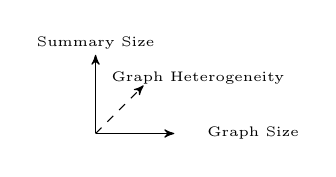
\begin{tikzpicture}[->,>=stealth']
\draw (0,0) -- (1,0);
\draw (0,0) -- (0,1);
\draw[dashed] (0,0) -- (.61,.61);

\node (a) at (2,0) {{\tiny Graph Size}};
\node (b) at (0,1.15) {{\tiny Summary Size}};
\node (c) at (1.3,.71) {{\tiny Graph Heterogeneity}};
\end{tikzpicture}
	}
	\caption{Graph summarisation dimensions}
	\label{fig:gs-axis}
\end{figure}

\paragraph{Size of the graph.}

It is desirable for a summary to be smaller than the graph, since it is generally a substitute of the original data graph for performance reason. We measure the ``complexity'' of a graph by its number of edges. The rationale is that the more a graph has edges, the more difficult it is to process since it requires more computational power and memory.
%We introduce the \emph{volume} as a way for measuring how complex a graph is, and is computed from the numbers of nodes and edges in the graph.
%
%\begin{definition}[Graph Volume]
%Let $G=\left\langle V, A, l_V \right\rangle$ be a graph.
%We call $Vol(G)$ the \emph{volume} of the graph $G$, and is equal to the sum of the size and order of $G$:
%$$
%Vol(G) = \vert A \vert + \vert V \vert
%$$
%\end{definition}

\paragraph{Graph heterogeneity.}

We consider a graph to be heterogeneous when it is not consistent with regards to
\begin{inparaenum}[(a)]
\item its structure; and
\item its labelling.
\end{inparaenum}
Our rationale is that the more heterogeneous a graph is, the more difficult it is to create a \emph{precise} and \emph{concise} description of that graph. For example, we can imagine a dataset describing people in which the attributes are not consistent from a person to an other: for one the phone number is missing, while for an other it is the birth place. The Figure~\ref{fig:graph-hetero} illustrates the two scenari of graph heterogeneity, where we depict possibles graph summarisation with a \textit{dashed} graph.

\subparagraph{Heterogeneity of the graph structure.}

Figure~\ref{fig:hetero-struct} depicts a graph in which the structure is inconsistent. The node $a_0$ has two incoming edges and a single outgoing edge, while for the node $b_0$ it is the opposite: a single incoming edge and two outgoing. Although the depicted summary in dashed lines may be considered sufficient, it loses some \emph{information} about the graph. We may record the in/out-degrees as \emph{metadata} but this requires additional storage space.

\subparagraph{Heterogeneity of the vocabulary.}

Considering our previous example of the people dataset, a graph can be seen as heterogeneous if it uses different attributes for each entity within. Figure~\ref{fig:hetero-voc} depicts a graph in which this is the case: entities $a_1$, $\cdots$, $a_n$ have a different attribute each. A possible summarisation would be to create an isomorph graph, but then the summarisation purpose that is to substitute the graph with an other more manageable is lost. An other summarisation is depicted on the right as a dashed graph, where two nodes $s_a$ and $s_b$ are linked with all $n$ attributes. Although this reduces the number of nodes to from $2 \times n$ to $2$, we loose the original distribution of the attributes.\\

In the rest of this chapter, we discuss the graph summarisation literature with regards to the three axes.

\begin{figure}
	\centering
	\begin{subfigure}{.5\textwidth}
		\resizebox{\textwidth}{!}{
			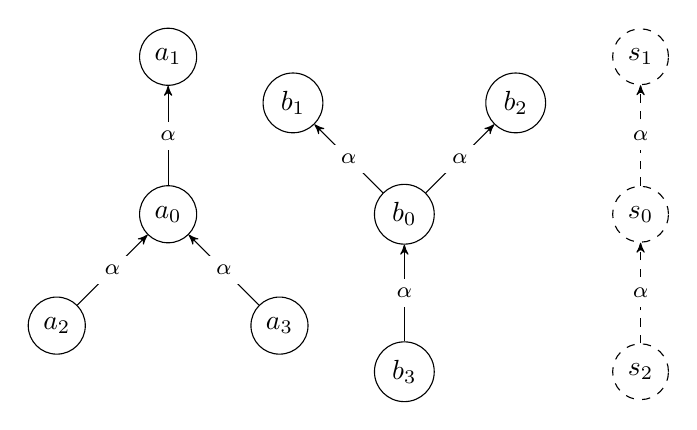
\begin{tikzpicture}[->,node distance=2cm,>=stealth']
\node[draw,circle] (a0) {$a_0$};
\node[draw,circle,above of = a0] (a1) {$a_1$};
\node[draw,circle,below left of = a0] (a2) {$a_2$};
\node[draw,circle, below right of = a0] (a3) {$a_3$};

\path[every node/.style={fill=white,font=\footnotesize}]
(a0) edge node {$\alpha$} (a1)
(a2) edge node {$\alpha$} (a0)
(a3) edge node {$\alpha$} (a0)
;

\node[draw,circle,right of = a0,xshift=1cm] (b0) {$b_0$};
\node[draw,circle,above left of = b0] (b1) {$b_1$};
\node[draw,circle,above right of = b0] (b2) {$b_2$};
\node[draw,circle, below of = b0] (b3) {$b_3$};

\path[every node/.style={fill=white,font=\footnotesize}]
(b0) edge node {$\alpha$} (b1)
(b0) edge node {$\alpha$} (b2)
(b3) edge node {$\alpha$} (b0)
;

% summary
\node[dashed,draw,circle,right of = b0,xshift=1cm] (s0) {$s_0$};
\node[dashed,draw,circle,above of = s0] (s1) {$s_1$};
\node[dashed,draw,circle, below of = s0] (s2) {$s_2$};

\path[every node/.style={fill=white,font=\footnotesize}]
(s0) edge[dashed] node {$\alpha$} (s1)
(s2) edge[dashed] node {$\alpha$} (s0)
;
\end{tikzpicture}
		}
		\caption{Graph structure heterogeneity}
		\label{fig:hetero-struct}
	\end{subfigure}
	\qquad
	\begin{subfigure}{.42\textwidth}
		\resizebox{\textwidth}{!}{
			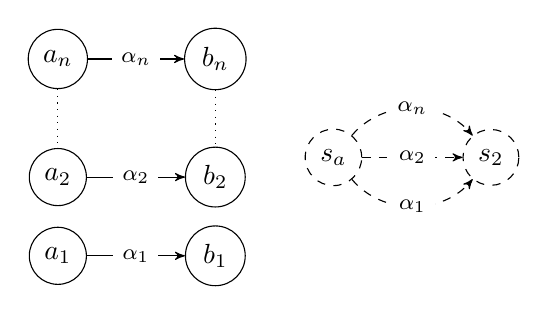
\begin{tikzpicture}[->,>=stealth']
\node[draw,circle] (a1) {$a_1$};
\node[draw,circle,right of = a1,xshift=1cm] (b1) {$b_1$};

\node[draw,circle,above of = a1] (a2) {$a_2$};
\node[draw,circle,right of = a2,xshift=1cm] (b2) {$b_2$};

\node[draw,circle,above of = a2,yshift=.5cm] (an) {$a_n$};
\node[draw,circle,right of = an,xshift=1cm] (bn) {$b_n$};

% summary
\node[dashed,draw,circle,right of = b2,xshift=.5cm,yshift=.25cm] (sa) {$s_a$};
\node[dashed,draw,circle,right of = sa,xshift=1cm] (sb) {$s_2$};

\path[every node/.style={fill=white,font=\footnotesize}]
(a1) edge node {$\alpha_1$} (b1)
(a2) edge node {$\alpha_2$} (b2)
(an) edge node {$\alpha_n$} (bn) edge[-,dotted] (a2)
(bn) edge[-,dotted] (b2)
(sa) edge[dashed,bend right=50] node {$\alpha_1$} (sb)
(sa) edge[dashed] node {$\alpha_2$} (sb)
(sa) edge[dashed,bend left=50] node {$\alpha_n$} (sb)
;
\end{tikzpicture}

		}
		\caption{Graph vocabulary heterogeneity}
		\label{fig:hetero-voc}
	\end{subfigure}
	\caption{Graph heterogeneity where the dashed graphs represent possible summaries of the graph}
	\label{fig:graph-hetero}
\end{figure}

\section{Graph Summarisation Approaches}

%% present here the different kinds of approaches
The concept of graph summarisation has been explored for diverse use cases in the literature. As discussed in Section~\ref{chap03:review:query-optim}, graph summarisation has been used for the purpose of optimising the query evaluation by outlining what paths exist in the graph and creating indices over the summary. In Section~\ref{chap03:review:graph-exploration}, we present some research where it has been employed also for aiding a user in exploring an unknown graph. In Section~\ref{chap03:review:query-profiling}, a summary of the graph is used for profiling the data, i.e., gathering some statistics about the graph so to analyse it with regards to upstream applications such as data integration. Graph summarisation is also used for analysing the \emph{content} of the graph by computing aggregates, which research is discussed in Section~\ref{chap03:review:data-analytics}.

Figure~\ref{fig:timeline} depicts a timeline of the literature presented in this chapter. The main use case of each work is indicated with a color and shape-coded arrow and reflect the sections outlined in the previous paragraph. From the timeline, we can see that graph summarisation was at first used for optimising query evaluation through indices; a new direction later appeared where the summary is used for analysing and exploring a graph. This new direction might be linked with the emergence of Web Data, since users generally interact with graphs which structure is (partially) unknown.

\paragraph{Graph clustering versus graph summarisation.}

Both techniques are similar in the sense that they partition the graph.
Clustering is the process of finding the underlying structure of a dataset by grouping elements that are \emph{similar} to each other. A group is then called a cluster. In the context of a graph, a clustering technique seeks clusters of nodes that have many connections to each other \emph{within}, but few \emph{between} the clusters. Schaeffer presents in \cite{schaeffer:2007:graph} a survey of graph clustering approaches. Instead, with graph summarisation techniques we aim to partition the graph in such a way that the original structure of the graph is preserved.

\paragraph{Fundamental vocabulary.}

Given a graph $G = \left\langle V, A, l_V \right\rangle$, the process of graph summarisation creates an other graph, called the \emph{summary} of $G$. Each node of $G$ is mapped to one or more nodes of the summary, which we call as the \emph{sumnodes}. Similarly, edges of the graph $G$ are also mapped to edges in the summary, which we call the \emph{sumedges}. The goal of the graph summarisation is to create a summary where the structure of the original graph $G$ is preserved.

\begin{figure}
	\resizebox{\textwidth}{!}{
		\begin{timeline}{1997}{2014}{1cm}{2cm}{16cm}{\textheight}
			\entry{1997}{DataGuides improves the query execution thanks to an index of the summary \cite{goldman1997dataguides}.}{red, dashed}
			\entry{1999}{Approximation of DataGuides \cite{goldman1999approximate}.}{red, dashed}
			\entry{1999}{The index proposed in \cite{Milo:1999:ISP:645503.656266} allows to summarize specific paths.}{red, dashed}
			\entry{2002}{In the same spirit of \cite{Milo:1999:ISP:645503.656266}, the summary index is created given a query \cite{kaushik:de:2002,kaushik:2002:cib}.}{red, dashed}
			\entry{2003}{The summarisation approach in \cite{chen:2003:dia} adapts itself to the query load.}{red, dashed}
			\entry{2008}{Tian et. al \cite{tian:sigmod:2008,zhang:2010:ddg} present a summarisation approach that bridges to OLAP (Online analytical processing) with drilldown/rollup operations.}{blue}
			\entry{2008}{Navlakha et. al \cite{navlakha:2008:gsb} propose a summarisation approach based on Information Theory, where the end result is a summary and a set of corrections. This allows to recreate the original graph from the summary with a bounded error.}{decorate with=diamond, paint=black, decoration={shape evenly spread=8}}
			\entry{2008}{\cite{chen:icdm:2008}.}{green, very  thick,  dotted}
			\entry{2010}{\cite{khatchadourian:2010:eswc}.}{decorate with=diamond, paint=black, decoration={shape evenly spread=8}}
			\entry{2011}{\cite{zheng:ipsj:2011}}{blue}
			\entry{2011}{\cite{qu:dasfaa:2011}}{green, very  thick,  dotted}
			\entry{2011}{\cite{zhao:sigmod:2011}.}{green, very  thick,  dotted}
			\entry{2012}{Tran et. al \cite{Tran:2012:kde} group similarly structured graphs together so to decrease the communication cost of join operations.}{red, dashed}
			\entry{2012}{Konrath et. al \cite{konrath:jws:2012} suggest a dataset from its structure in which a SPARQL query is more likely to yield results.}{blue}
			\entry{2012}{A distributed graph summarisation approach based on ``message passing'' \cite{liu:cikm:2014}}{black}
			\entry{2013}{\cite{rudolf:2013:slg}.}{green, very  thick,  dotted}
			\entry{2014}{Riondato et. al \cite{riondato:2014:gsq} present an approach which minimises error in reconstructing the graph from summary.}{red, dashed}
			\entry{2014}{\cite{colazzo:www:2014}.}{green, very  thick,  dotted}
			\entry{2014}{\cite{zhengkui:2014:ppg}.}{green, very  thick,  dotted}
			\legend{red, dashed}{Query Optimisation}
			\legend{blue}{Graph Exploration}
			\legend{decorate with=diamond, paint=black, decoration={shape evenly spread=2}}{Data Profiling}
			\legend{green, very  thick,  dotted}{Data Analytics}
			\legend{black}{Large-scale Computation}
		\end{timeline}
	}
	\caption{Timeline of the research on graph summarisation}
	\label{fig:timeline}
\end{figure}

\section{Graph Exploration}
\label{chap03:review:graph-exploration}

Graph summarisation techniques can be used for exploring a graph. In this scenario, the structure of the graph is (partially) unknown; it is necessary in order to compose queries over the graph. The user leverage the summary to learn what attributes are used, what classes, how they relate with each other.\\

Tian et. al \cite{tian:sigmod:2008} propose the use of graph summarisation for exploring a graph: by grouping nodes that share some pre-defined criteria, the ``general'' structure of the graph is brought out. The coarseness of the grouping can also be tuned so to retain more or less details about the graph. This work is a bridge to the OLAP (online analytical processing) world, since it allows OLAP-style exploration of the graph by providing drill-down and rollup operations. The user can drill-down, i.e., view more details about the graph's structure, and rollup, i.e., browse a more abstract view of the graph's structure, over the graph. This is made possible by showing a \emph{summary} of the graph at each level of detail in the drill-down/rollup exploration.

The proposed approach creates a summary graph by mapping each node of the graph into exactly one sumnode; several nodes can map to a same sumnode in the summary. Two nodes are mapped to a same sumnode if they share the same
\begin{inparaenum}[(a)]
	\item attributes' value; and
	\label{acompatible}
	\item incident sumnodes of the sumnode a node maps to.
	\label{rcompatible}
\end{inparaenum}
The algorithm first partition the graph in order to achieve (\ref{acompatible}), then iteratively splits each block (sumnode) in the partition until each node in a sumnode fulfil (\ref{rcompatible}). The latter relies on the incident matrix between nodes in the graph and sumnodes in the summary in order to split a sumnode or not; there is one such matrix per attribute. A cell $a_{i,j}$ of the matrix is equal to $1$ if a node on row $i$ maps to a sumnode which is a neighbour of the sumnode on column $j$.

The algorithm requires several passes over the graph in order to fulfil (\ref{rcompatible}). For large graphs that do not fit in memory, this becomes a challenge in itself. Indeed, if some part of the graph is not in memory, it needs to be retrieved, e.g., from disk, which would impact negatively on the algorithm performance.

The authors extend this work in \cite{zhang:2010:ddg} where a measure for the ``interestingness'' of a graph summary is proposed. The aim of this measure is to quantify how easy it is for a person to visualise and understand the high-level structural characteristics of the graph. In Section~\ref{chap03:sec:quality}, we argue that the interestingness of a summary actually depends on the application it is used for. In that paper, the authors also investigate how to summarise numeric data; while this is an important aspect of graph summarisation in some application, we focus in this thesis on summarising the structure of the graph.\\

Liu et. al \cite{zheng:ipsj:2011} propose a graph summarisation that \emph{approximates} the information in the original graph, i.e., the structure of the graph and the attributes' value associated with a node. The authors aim to construct a summary that is \emph{homogeneous}, i.e., each node mapped to a sumnode of the summary are consistent with one an other. Three criteria that measure different aspect of the summary homogeneity are introduced:
\begin{itemize}
	\item all nodes mapped to the a sumnode have the \emph{same} attributes' value;
	\item a sumedge $(a,b)$ implies that \emph{all} nodes in the sumnode $a$ are connected to at least on node in $b$; and
	\item all nodes mapped to the a sumnode must have the same \emph{degree}\footnote{Degree is the number of nodes adjacent to a node.}.
\end{itemize}
The quality of a criterion is measured using the entropy. A summary built with all three criteria fulfilled can be approximated --- so to achieve a smaller size --- by relaxing a criterion.

Two algorithms are presented for creating an approximate summary. The first one is an agglomerative approach which starts from the \emph{exact} graph partition according to the three criteria, then proceeds to merge sumnodes until reaching a pre-defined number of sumnodes. At each iteration, the merged sumnodes are those that would results in minimal entropy. The second algorithm instead relies on a K-Means clustering of the graph and \emph{split} sumnode until a pre-defined number of sumnodes is reached. The first algorithm presents the challenge of starting from the exact partition, which is computationally expensive as it requires several iterations over the graph. Both algorithms use a pre-defined number of sumnodes, although a user probably has no idea what number to choose.\\

The authors in \cite{konrath:jws:2012} propose a three-layer index on top of the Linking Open Data (LOD). Each layer provides a view on the data with varying details. Ultimately, the index allows to select data sources that are relevant for a SPARQL query. The selection is driven by the three layers of the index, where each is more suited to a query of specific complexity.
Each layer of the proposed index provides views of the LOD graph with varying granularity: the lower the layer, the more detailed it is. A layer can be considered as a possible summarisation of the LOD graph, although connections between sumnodes within a layer is not provided. The proposed index model is then orthogonal to our graph summarisation model, each layer being a summary itself.
We note that the third layer which is the most detailed one is based on \emph{bisimulation}; however, the definition used in that work is not the commonly used one, which we present in Section~\ref{chap:summary:bisim}.

%\begin{itemize}
%\item \cite{tian:sigmod:2008} proposes an approach based on bisimulation that provides more or less detailed summaries. However, the level of detail is left to the user; this assumes some  prior knowledge about the data structure and content. Bridge between OLAP and graph summarisation.

%- support for multi-valued attributes: essential for rdf:types
%- the attributes' value are also taken into consideration when creating groups of nodes.
%  - ex of 2 graphs with different attribute values but similar graph structure.
%  - for web data, this can increase the size of the summary
%- only direct relationships are considered for grouping nodes.
%- can be modelled using our approach as it is a graph homomorphism.
%- Iteration approach: initialise grouping based of A-compatible, then split groups until the grouping is (A,R)-compatible.
%- neighbor group bitmap is the incidence matrix between nodes and group. There is such a matrix for each edge label ~~ with heterogeneity.

%* nodes - LB=nb of distinct attributes' value groups	UB=nb of nodes orig

%\item \cite{zhang:2010:ddg} addresses two shortcomings of \cite{tian:sigmod:2008} by supporting numerical data and proposing an ``interestingness'' measure of a graph summary. That measure helps a user to find the best resolution of the summary.

%\item An Information Theoretic approach to graph summarisation is presented in \cite{zheng:ipsj:2011}. The authors propose three criteria for defining the homogeneous property of a graph. A criterion can then be relaxed in order to produce a smaller (approximate) graph summary. The technique seeks to lower the entropy of the graph summary, hence ensuring a good quality.
%\end{itemize}

\section{Data Profiling}
\label{chap03:review:query-profiling}

Khatchadourian et. al \cite{khatchadourian:2010:eswc} describe the graph's structure along with statistics thanks to summaries. The proposed summary is built using the bisimulation equivalence, which is described in Section~\ref{chap:summary:bisim}. The presented approach is tailored towards RDF graphs; instead, we present a graph summarisation framework that is independent of the graph modelling.

The authors consider a node-only labelled directed graph: each label in our graph model presented in Section~\ref{sec:gdm:formal-model} forms a node. We use instead the same graph model for both the original graph and for the summary graph, thus simplifying the framework.
The labelling scheme proposed in \cite{khatchadourian:2010:eswc} of sumnodes and sumedges is limiting, since it considers only parts of the resources' URI in the original graph, e.g., the localname. The set of labels thus constructed is too small for finely controlling how much information from the graph is retained. To add more flexibility, we decouple the definition of a node from the creation of its label, where the former is discussed in Section~\ref{chap:summary:model} and the latter in Section~\ref{chap:summary:algo}.
The authors discuss the summarisation of \emph{inter-linked} datasets through the use of specific labelled edges, i.e., \emph{owl:sameAs} edges. Instead, we consider in this scenario the context of the graphs, which we detail in Section~\ref{chap03:summary:impl:inter-datasets}.\\

Navlakha et. al \cite{navlakha:2008:gsb} propose a graph summarisation approach based on Information Theory. The result of the approach is the creation of two data structures, i.e., the summary graph and a set of corrections. The set of corrections allows to rebuild the original graph by correcting any error in the summary graph, e.g., a sumedge exists in the summary that links two \emph{disconnected} nodes in the original graph. The algorithm is based on the minimum description length \cite{grunwald:2007:mdl} principle which aims to minimise the cost of the summary representation of the graph, i.e., the sum of the summary's size and of the corrections' set size.
The size of the summary can be further reduced by allowing some errors; there is then a trade-off between the precision and the size of the summary. In contrary, we do not attempt to rebuild the original graph from the summary and so we focus on summarising the structure of the graph.

%\begin{itemize}
%\item A system for the discovery of datasets is proposed in \cite{khatchadourian:2010:eswc}.
%- the presented approach is tailored towards RDF graphs. we present a graph summarisation model that is independent of the graph modelling.
%- the labelling scheme is limiting, it considers only parts of the URI, e.g., the localname. the set of labels for the sumnodes and sumedges is too small for controlling how much information from the graph is retained. (explain pb with available\_as)
%- discuss summary of inter-linked datasets based on sameas links. instead we consider the context of statements when summarising inter-linked datasets.
%\item The authors of \cite{navlakha:2008:gsb} propose a summarisation based on the Information Theory principle of Minimum Description Length. Although the original data graph can be re-created from the summary, a user-defined bounded error parameter can be used to balance the summary volume with the loss in precision.
%\end{itemize}

\section{Data Analytics}
\label{chap03:review:data-analytics}

OLAP (online analytical processing) is a technique for answering analytical queries over multi-dimensional data. Through various operations it allows a user to analyse the data from different perspectives. Each perspective is called a \emph{cube}, obtained by aggregating the values of some dimensions.

Several works investigate the use of OLAP over graphs: data records analysed through OLAP are now related to each other. The main difference between traditional OLAP and graph-OLAP is the \emph{measure} which traditionally is a number becomes a \emph{graph}. Compared to \cite{tian:sigmod:2008} discussed in Section~\ref{chap03:review:graph-exploration}, the works presented here are anchored in a OLAP background, rather than being a bridge to OLAP from the graph exploration domain.

Among the possible OLAP operations, \emph{rollup} and \emph{drill-down} control the level of details presented to the user about the graph. With regards to our graph summarisation presented in Chapter~\ref{chap:summary}, each level is actually a summary. Therefore, the approaches of OLAP over graphs are orthogonal to ours.\\

Chen et. al propose in \cite{chen:icdm:2008} two OLAP frameworks \emph{I-OLAP} and \emph{T-OLAP} for analysing graphs. The I-OLAP aggregation is aimed at summarising various graphs representing a same entity. It is then a merge of the graphs that keeps the entity layer, while we rather consider the summarisation of the graph's structure which is a different view on the graph. The T-OLAP framework, which is further investigated in \cite{qu:dasfaa:2011}, modifies the \emph{topology} of the graph. T-OLAP maps nodes into sumnodes according to their attributes' value, and computes a statistic for the sumnode using an aggregate function, e.g., \emph{count}. Compared to our graph summarisation, the authors consider the attributes' value while we do not require those.\\

Zhao et. al \cite{zhao:sigmod:2011}.

\begin{itemize}
\item Colazzo et al. \cite{colazzo:www:2014} describe a framework for using OLAP over RDF data, leveraging the rich structure of such graphs. Each cube is built based on SPARQL queries which define supernodes and superedges. This analytical framework is flexible enough to accommodate various kinds of analysis, since the aggregate function is also based on a SPARQL query. Although the analysis of the data is done through its cubes by a user, the computation of a cube is always done over the original data. The need of writing SPARQL queries suggests that a user possesses some knowledge about the structure of the graph. This work is orthogonal to the one proposed in this thesis: our approach highlights the graph structure, thanks to which a deeper analysis of the graph can be done.
\item Zhengkui et al. generalise the concept of OLAP over graphs in \cite{zhengkui:2014:ppg} by proposing an property graph model and allowing to summarise over the edges and/or nodes properties. The approach is implemented over a MapReduce framework. It leverage the lattice graph of the summaries to process several aggregations in a single job. A best execution plan for the series of MapReduce jobs is found using a cost model.
\item SAP proposes to analyses graphs through user-defined summarisation in \cite{rudolf:2013:slg}.
\end{itemize}

\section{Query Optimisation}
\label{chap03:review:query-optim}

\begin{itemize}
\item DataGuides \cite{goldman1997dataguides} is the first work to improve query execution through the use of an index on the summary of the structure of the graph. However, the DataGuides construction algorithm is computationally expensive. Also, in presence of data with a complex structure, the size of the summary can be as large as the data graph, or even larger. This issue is discussed in \cite{goldman1999approximate}, where some constraints of DataGuides are relaxed, e.g., the existence of a path in the data graph.
\item \cite{Milo:1999:ISP:645503.656266} extends the work on DataGuides, using the notion of bisimulation to build a structure index. The authors propose to reduce further the size of a summary by defining the type of query to answer. However, it assumes some knowledge about the structure of the data graph in order to specify the query type. Also, any change in the query specification requires to rebuild the summary.
\item In \cite{kaushik:de:2002} the definition of bisimulation on a graph is simplified by limiting the length of a path to $k$ hops. In \cite{kaushik:2002:cib} the authors create an index of paths expressions, based on a summary that has been build for a pre-defined query expression.
\item In \cite{chen:2003:dia}, the authors vary the maximum length of a path per node, depending on the query load of the system.
\item The authors of \cite{Tran:2012:kde} uses a similar approach to \cite{kaushik:2002:cib} for the purpose of improving the partitioning of RDF data and the execution of queries. Tran et al. partition the data into groups having a similar structure in order to reduce communication load and the number of joins.
\item Rondiato et al. present in \cite{riondato:2014:gsq} a graph summarisation approach that bridges to graph clustering. The summarisation is expressed as an optimisation, where an error function is to be minimised. The error function is expressed as the distance between the adjacency matrices of the graph and its summary. The number of nodes in the summary is set as a parameter to the algorithm.
\end{itemize}

\section{Summarisation for Graph Schema Rendering}

\section{Graph Summarisation Quality}

The index creation in \cite{konrath:jws:2012} is a stream-based approach. The authors investigate then the impact of the window size on the quality of the created index. However, the authors do not investigate the quality with regards to the structure of the data graph summarised by the index.

\section{Large-scale Computation}
\label{chap03:review:large-scale-comp}

In order to deal with large graphs, distributed implementations of graph summarisation has been researched.
Liu et al. in \cite{liu:cikm:2014} present a graph summarisation approach based the \emph{Message Passing} paradigm: the algorithm iteratively merges nodes of the graph until a predefined number of nodes are left. Various solutions for selecting which nodes to merge are discussed, a method based on \emph{Locality Sensitive Hashing} is introduced. The merge process introduces errors with regards to the original graph, i.e., either missing or additional edges.

\subsection{Summary}

\begin{itemize}
\item algorithms with iterations
\item need to know the final number of sumnodes
\item graph summarisation approaches that consider attributes' value: T-OLAP in \cite{chen:icdm:2008}, SPAN in \cite{tian:sigmod:2008}. This is not mandatory in our framework.
\item our graph summarisation framework is flexible in the summary construction, since it is based on graph homomorphism and the definition of the relation is left to the user.
\end{itemize}


\part{Methods}

%%
%% graph summary
%%

\chapter{Graph Summary: a Novel Schema for Web Data}
\label{chap:summary}

The Web Data consists of a tremendous amount of structured datasets, coming from a variety of sources. An attractive aspect of the Web Data is the total freedom with regards to the production of ``knowledge''; as stated by Berners-Lee in~\cite{tbl:1997:wam}, ``Anyone can say anything about anything''. Undoubtedly, the facility to publish data played a role in the considerable growth of the Web Data. However, this also means that there is nothing enforcing some \emph{quality} of the data, e.g., what design structure or vocabulary terms to use, or checking data consistency.

Although there exists a number of ontologies for describing a wealth of data, datasets do not follow strictly the specifications. Enforcing the structure would stand against the design choice of the Web Data stated above. Another approach is to go with the flow and \emph{generate} such specifications directly from the data itself.

Graph summarisation is a technique that maps an entity graph into another, \emph{smaller} graph. That new graph keeps the same \emph{structure} as the entity graph, but contains less nodes and less edges. % The new graph defines then a \emph{schema} of the graph.
As we aim to highlight the underlying structure of a graph, we consider already existing features for the summarisation, built alongside the graph. Such features are for example the \gls{attributes} and \gls{types} of a graph.
In this chapter, we present how to summarise graphs in the context of Web Data.


\section{Graph Summarisation}
\label{chap:summary:model}

Web Data contains a large amount of structured data spanning over many different domains, from information on movies to the description of genes. There are billions of statements and millions of entities. There is a wealth of vocabulary terms for every kind of data, which are used more or less in the way a vocabulary was design for.

In order to make sense of this deluge of data, summarisation techniques are available for different levels of the data. For example, all the information related to an entity can be summarised so to highlight the important parts. In this section, we are interested in the summarisation of the \emph{structure} of graphs. In the context of Web Data, the structure of a graph is defined by the use of predicates and classes.

We present first a model for graph summarisation. Then, we emphasise the direction of \emph{approximate} graph summarisation as the only viable summarisation for Web Data in many cases. Finally, we describe how inter-linked datasets can be summarised.

\cite{Milner:1989:CC:534666} introduces the concept of bisimulation to define equivalent processes in concurrent systems. The relational coarsest partition \cite{Paige:1987:TPR:37185.37186} is generally the algorithm used for computing a bisimulation on a graph.

\subsection{Model}

In this section, we present a formal model of graph summarisation.

\paragraph{Properties of a Summary.}

Graph summarisation is an operation over the graph that abstracts from its content, in order to highlights its structure. From a structural point of view, traversing a graph or its summary is equivalent. The summary of a graph exhibits the following properties:
\begin{enumerate}
	\item a path in the graph exists also in the summary;
	\label{sprop-path}
	\item both the graph and its summary share the same vocabulary; and
	\label{sprop-voc}
	\item a graph may conform to several summaries.
	\label{sprop-not-uniq}
\end{enumerate}
These properties of a summary are fulfilled by defining the graph summarisation as a graph \emph{homomorphism}.

\paragraph{Graph homomorphism.}

A graph is homomorph to another one if there exists a mapping of nodes that matches \emph{edges} from the first to the second graph. This ensures that the structure of the first graph is kept.
The Figure~\ref{fig:homomorphism} depicts two graphs, where there exists a relation $R$ that maps nodes of the left graph to nodes of the right graph. The edges of the left graph are also kept in the right graph. Indeed, there is an edge from nodes $2$ and $3$ to $1$, and as well there is an edge between their mapped nodes, $a$ and $b$ respectively.

\begin{definition}[Graph Homomorphism]
	Let $G=\left\langle V, A, l_V \right\rangle$ and $\mathcal{S}=\left\langle \mathcal{W}, \mathcal{B}, l_\mathcal{W} \right\rangle$ be two graphs. Let $R \subseteq V \times \mathcal{W}$ be a binary relation.
	In the context of the binary relation, $G$ is homomorphic to $\mathcal{S}$ if every edge in $G$ is \emph{mapped} to an edge in $\mathcal{S}$:
	$$
	\forall (u, \alpha, v) \in A\;\; \forall (x, y) \in \mathcal{W}\;\; (u, x) \in R \wedge (v, y) \in R \implies (x, \alpha, y) \in \mathcal{B}
	$$
	We say that $G$ is homomorphic to $\mathcal{S}$.
\end{definition}

A graph homomorphism is defined by a many-to-many binary relation $R$ from the nodes $V$ to the nodes $\mathcal{W}$, and that for every edge in $A$ there is a corresponding edge in $\mathcal{B}$. Whenever two nodes in the graph $G$ are linked by a predicate $\alpha$, then so are their corresponding nodes in the graph $\mathcal{S}$.\\

\begin{figure}
	\centering
	\usetikzlibrary{arrows}

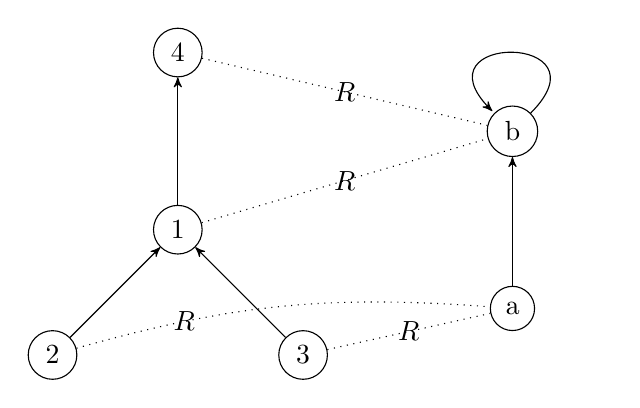
\begin{tikzpicture}[>=stealth',node distance=2.25cm]
\node [draw,circle] (1) {1};
\node [draw,circle,below left of = 1] (2) {2};
\node [draw,circle,below right of = 1] (3) {3};
\node [draw,circle,above of = 1] (4) {4};

\node [draw,circle,right of = 1,xshift=2cm,yshift=-1cm] (a) {a};
\node [draw,circle,above of = a] (b) {b};

\path (1) edge[->] (4)
		   (2) edge[->] (1)
		   (3) edge[->] (1)
		   (a) edge[->] (b)
  		   (b) edge[->,loop] (b)
		   (1) edge [dotted] node {$R$} (b)
		   (4) edge [dotted] node {$R$} (b)
		   (2) edge [dotted,bend left=10] node[near start] {$R$} (a)
		   (3) edge [dotted] node {$R$} (a);
\end{tikzpicture}
	\caption{Graph homomorphism. There is a relation $R$ that maps nodes of the left graph to the nodes of the right graph which keeps the connection of the right graph.}
	\label{fig:homomorphism}
\end{figure}

\paragraph{Graph summary.}

We call a graph $\mathcal{S}$ for which a graph $G$ is \emph{homomorphic} to --- the \emph{summary} of $G$ \cite{campinas:2012:dexa}. Indeed, the summary being homomorph to $G$ retain by definition the paths in the graph described in the property~(\ref{sprop-path}). Both graph share the set of labels $\mathcal{L}$, thus meeting the property~(\ref{sprop-voc}) of a summary.

\begin{definition}[Graph Summary]
Let $G=\left\langle V, A, l_V \right\rangle$ and $\mathcal{S}=\left\langle \mathcal{W}, \mathcal{B}, l_\mathcal{W} \right\rangle$ be two graphs such that their set of nodes are distinct, i.e., $V \cap \mathcal{W} = \emptyset$. Both graphs share the same set of labels $\mathcal{L}$. Let $R \subseteq V \times \mathcal{W}$ be a binary relation, and we call $R$ the \emph{summarisation relation}.
If $G$ is homomorphic to $\mathcal{S}$ then the graph $\mathcal{S}$ is a summary of $G$.
\end{definition}

\begin{remark}
From this point on, we shall differentiate between the nodes and edges of $G$ from those of $\mathcal{S}$ by calling a node of the summary a \emph{sumnode}, and an edge a \emph{sumedge}. Unless stated explicitly, the terms node and edge refer to the components of the entity graph $G$.
\end{remark}

Figure~\ref{fig:basic-summary} depicts a possible summary for a graph. The dotted lines illustrate the summarisation relation $R$, where we have for example $(a, S_1) \in R$ and $(John, S_3) \in R$.

\begin{figure}
	\centering
	\resizebox{.7\textwidth}{!}{
		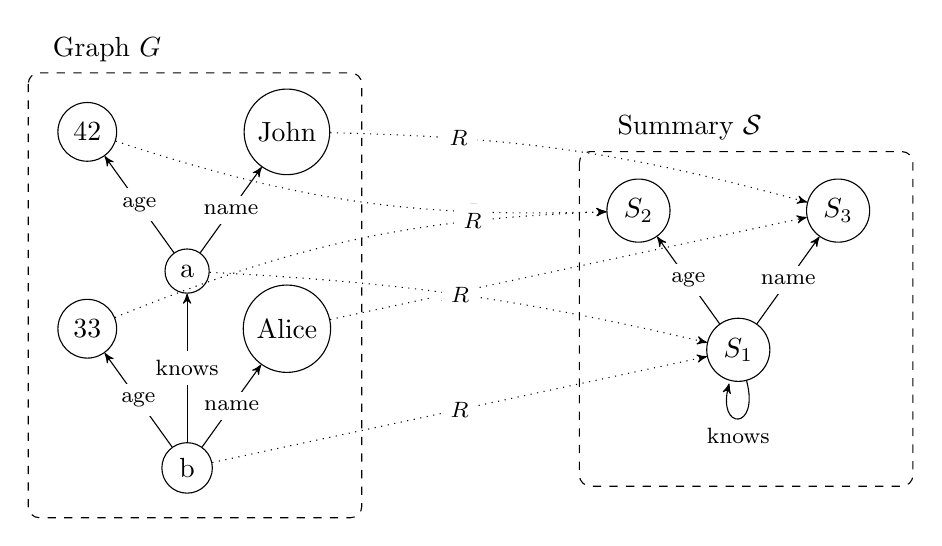
\begin{tikzpicture}[>=stealth',->,node distance=2.5cm]
%% graph
\node[draw,circle] (a) {a};
\node[draw,circle,above left of = a,xshift=.5cm] (aage) {42};
\node[draw,circle,above right of = a,xshift=-.5cm] (aname) {John};

\node[draw,circle,below of = a] (b) {b};
\node[draw,circle,above left of = b,xshift=.5cm] (bage) {33};
\node[draw,circle,above right of = b,xshift=-.5cm] (bname) {Alice};

\coordinate (gx) at ($ (aage) + (-.75,.75) $);
\coordinate (gy) at ($ (bname) + (.95,-2.4) $);
\draw[rounded corners,dashed]  (gx) node[yshift=.3cm,xshift=1cm] {Graph $G$} rectangle (gy);

\path[every node/.style={fill=white,font=\footnotesize}]
(b) edge node {knows} (a)
(a) edge node {age} (aage)
(a) edge node {name} (aname)
(b) edge node {age} (bage)
(b) edge node {name} (bname)
;

%% summary
\node[draw,circle,right of = a,xshift=4.5cm,yshift=-1cm] (s) {$S_1$};
\node[draw,circle,above left of = s,xshift=.5cm] (sage) {$S_2$};
\node[draw,circle,above right of = s,xshift=-.5cm] (sname) {$S_3$};

\coordinate (sx) at ($ (sage) + (-.75,.75) $);
\coordinate (sy) at ($ (sname) + (.95,-3.5) $);
\draw[rounded corners,dashed]  (sx) node[yshift=.3cm,xshift=1.4cm] {Summary $\mathcal{S}$} rectangle (sy);

\path[every node/.style={font=\footnotesize}]
(s) edge[loop below] node {knows} (s)
(s) edge node[fill=white] {age} (sage)
(s) edge node[fill=white] {name} (sname)
;

\path[every node/.style={fill=white,font=\footnotesize},dotted]
(aage) edge[near end,bend right=10] node {$R$} (sage)
(bage) edge[bend left=10] node[near end] {$R$} (sage)
(aname) edge[near start,bend left=7] node {$R$} (sname)
(bname) edge node[near start] {$R$} (sname)
(a) edge[bend left=5] node {$R$} (s)
(b) edge node {$R$} (s)
;

\end{tikzpicture}
	}
	\caption{A graph and a possible summary. Dotted lines labelled $R$ represent the summarisation relation that maps nodes in the graph $G$ to sumnodes in $\mathcal{S}$.}
	\label{fig:basic-summary}
\end{figure}
%\begin{remark}
%Since the summarisation relation $R$ is a binary relation, we use the shorthand $R(u)$ to say that there exists a node $x \in \mathcal{W}$ such that $(u, x) \in R$, with $x = R(u)$.
%\end{remark}

%\begin{definition}[Graph Summary]
%Let $G=\left\langle V, A, l_V \right\rangle$ be a graph, and $R \subseteq V \times \mathcal{W}$ be a summarisation relation. The graph summary $\mathcal{S}=\left\langle \mathcal{W}, \mathcal{B}, l_\mathcal{W} \right\rangle$ of $G$ is defined as:
%\begin{enumerate}
%\item $\mathcal{W} = \left\lbrace y \mid (u,y) \in R \right\rbrace$;
%\item $\mathcal{B} \subseteq \left\lbrace \left(x, \alpha, y\right) \mid \exists (u,x) \in R \wedge \exists (v,y) \in R, \alpha \in \mathcal{L}^A \right\rbrace$.
%\end{enumerate}
%$l_\mathcal{W} : \mathcal{W} \mapsto \mathcal{L}_\mathcal{W}$ is a sumnode labelling function.
%\end{definition}

%\paragraph{Definition of a summary.}
%
%We use the symbol $\leftrightsquigarrow$ to express that a node of an entity graph $G$ is mapped to a sumnode of a summary $\mathcal{S}$ based on some features of the node.
%The Figure~\ref{fig:classes-summary} depicts a summary of the graph in the Figure~\ref{fig:graph} where the relation $R_t$ considers the set of types co-occurring in the graph. The table indicates the mappings by $R_t$ of the nodes in $V$, e.g., the nodes $N_1$ and $N_2$ are mapped to the sumnode $S_1$ since both connect to $Person$ via the type attribute. The summarisation relation $R_t$ is defined as:
%$$
%R_t = \left\lbrace (u, x) \in V \times \mathcal{W} \mid x \leftrightsquigarrow types(u) \right\rbrace
%$$
%\todo{review the definition of this notation. This may warrant a new definition.}

%The $\sim_t$-equivalence class ${[N_1]}^{\sim_t}$ contains the nodes $\left\lbrace N_1, N_2 \right\rbrace$ of $G$, since both connect to $Person$ via the type attribute.
%The concepts \emph{path}, \emph{type}, and \emph{attribute} introduced in the Section~\ref{sec:data-graph} hold for a summary.
%For example, we have for the node $[N_1]^{\sim_a}$ in the Figure~\ref{fig:attributes-summary} $types([N_1]^{\sim_a}) = \left\lbrace Person \right\rbrace$ and $attributes([N_1]^{\sim_a}) = \left\lbrace works, lives, name \right\rbrace$.
%\begin{definition}[Summary]
%Let $\sim$ be an equivalence relation and $G^\sim = \left\langle V^\sim, A^\sim, l_V^\sim \right\rangle$ be the $\sim$-summary of $G$, where $l_V^\sim$ be a $\sim$-equivalence class labelling function. The nodes $V^\sim$ are the $\sim$-equivalence classes on nodes of $G$ such that $V^\sim=\left\lbrace [x]^\sim : x \in V \right\rbrace$, with $[x]^\sim=\left\lbrace y \in V : y \sim x \right\rbrace$ the $\sim$-equivalence class of $x$. For every edge $x \overset{\alpha}{\rightarrow} y$ of $G$, there is an edge $[x]^\sim \overset{\alpha}{\rightarrow} [y]^\sim$ in $G^\sim$.
%\end{definition}

\paragraph{Partial relation.}

Depending on the definition of the summarisation relation $R$ some nodes of the graph do not have any mapping because they miss required features. For example, the node $N_0$ in Figure~\ref{fig:graph} does not have a $type$ edge; it has then no mapping for the previous relation $R_t$ that considers the set of types of a node as depicted in the Figure~\ref{fig:classes-summary}. As such, the relation $R$ is a \emph{partial relation}, where only a subset $V' \subseteq V$ has mappings; for the rest, it is \emph{undefined}. In the graph summary, we represent the set of undefined mappings with a sumnode labelled $\mathfrak{U}$.

\paragraph{Content abstraction.}

The purpose of a summary is to highlight the \emph{structure} of the graph, which is defined by the properties and types. Content information does not pertain the structure of the data, but only individual entities. Therefore, we abstract the summary from the content by mapping content nodes to a ``sink'' sumnode that we label as $\varnothing$. For example, the node labelled $Ireland$ in the Figure~\ref{fig:graph} is mapped to $\varnothing$. In RDF graphs, literals are mapped to the sink sumnode.


\begin{figure}
	\centering
	\begin{minipage}{.7\textwidth}
		\resizebox{\textwidth}{!}{
			\usetikzlibrary{arrows}

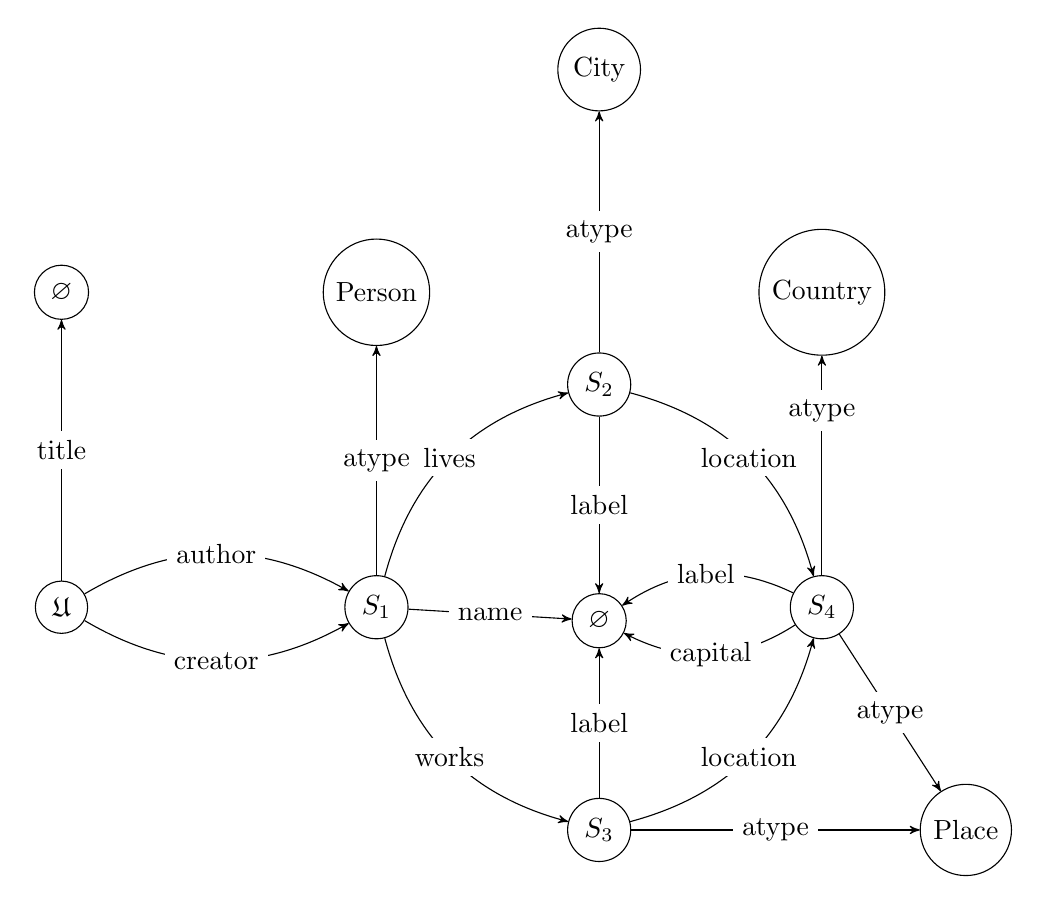
\begin{tikzpicture}[->,>=stealth',node distance=4cm]
\node [draw,circle] (b) {$\mathfrak{U}$};
\node [draw,circle,right of = b] (h1) {$S_1$};
\node [draw,circle,above right of = h1] (h2) {$S_2$};
\node [draw,circle,below right of = h1] (h3) {$S_3$};
\node [draw,circle,above right of = h3] (h4) {$S_4$};
\node [draw,circle,above of = h1] (person) {Person};
\node [draw,circle,above of = h2] (city) {City};
\node [draw,circle,above of = h4] (country) {Country};
\node [draw,circle,below right of = h4,xshift=-1cm] (place) {Place};
\node [draw,circle,above of = b] (c1) {$\varnothing$};
\node [draw,circle,below of = h2,yshift=1cm] (c2) {$\varnothing$};

\path
(b) edge node[fill=white] {title} (c1)
(h1) edge node[fill=white] {name} (c2)
(h3) edge node[fill=white] {label} (c2)
(h2) edge node[fill=white] {label} (c2)
(h4) edge[bend right] node[fill=white] {label} (c2)
(h4) edge[bend left] node[fill=white] {capital} (c2)

(h1) edge node[fill=white] {\glssymbol{atype}} (person)
(h2) edge node[fill=white] {\glssymbol{atype}} (city)
(h4) edge node[near end,fill=white] {\glssymbol{atype}} (country)
(h4) edge node[fill=white] {\glssymbol{atype}} (place)
(h3) edge node[fill=white] {\glssymbol{atype}} (place)
(h1) edge[bend left] node[fill=white] {lives} (h2)
(h1) edge[bend right] node[fill=white] {works} (h3)
(h2) edge[bend left] node[fill=white] {location} (h4)
(h3) edge[bend right] node[fill=white] {location} (h4)
(b) edge[bend right] node[fill=white] {creator} (h1)
(b) edge[bend left] node[fill=white] {author} (h1)
;
\end{tikzpicture}
		}
	\end{minipage}
	\quad
	\begin{minipage}[h]{.25\textwidth}
		\centering
		\caption*{$R_t\left(V, \mathcal{W}\right)$}
		\begin{tabular}{lc@{\hs}l}
			\toprule
			$V$ & \phantom{a} & $\mathcal{W}$ \\
			\cmidrule{1-1} \cmidrule{3-3}
			$N_0$ & \phantom{a} & $\mathfrak{U}$ \\
			$N_1$, $N_2$ & \phantom{a} & $S_1$ \\
			$N_3$ & \phantom{a} & $S_2$ \\
			$N_4$, $N_5$ & \phantom{a} & $S_3$ \\
			$N_6$, $N_7$ & \phantom{a} & $S_4$ \\
			\bottomrule
		\end{tabular}
	\end{minipage}
	\caption{Summary of the graph in Figure~\ref{fig:graph} with the summarisation relation $R_t$. The table indicates the mappings by $R_t$. The content in $G$ is abstracted by the sumnode $\varnothing$.}
	\label{fig:classes-summary}
\end{figure}

%We define the \emph{sink equivalence class} as the set of sink nodes, e.g., the node labelled $Ireland$ in the Figure~\ref{fig:graph} is part of this set. We remark that in the RDF data model, \emph{literals} are part of the sink equivalence class.
%\begin{definition}[Sink Equivalence Class]
%The set of sink nodes in $G$ is represented by the sink equivalence class $[\emptyset]=\left\lbrace x \in V : \not \exists (x, \alpha, y) \in A \right\rbrace$ in $G^\sim$.
%\end{definition}
%
%Depending on the $\sim$-equivalence, there can be nodes that do not have the required features to be assigned to a $\sim$-equivalence class. We define $B^\sim$ the \emph{blank $\sim$-equivalence class} as the set of such nodes of $G$, e.g., the node $N_0$ in the Figure~\ref{fig:graph} is assigned to the node $B^{\sim_t}$ in the Figure~\ref{fig:classes-summary}.
%\begin{definition}[Blank $\sim$-Equivalence Class]
%The set of nodes in $G$ for which there is no $\sim$-equivalent class is equal to the blank $\sim$-equivalence class $B^\sim$, i.e., $B^\sim=\left\lbrace x \in V : \forall y \in V, x \not \sim y \right\rbrace$.
%\end{definition}

\subsection{Precise Graph Summary}

The purpose of a summary is to mirror the structure of the graph while being significantly smaller. Therefore, the summary can substitute the graph and improve the performance of applications. How well the summary mirrors the graph is then of high importance. From a structural perspective, a summary is precise if it is undiscernable from the original graph.

Although the structure of the graph is preserved in the summary by definition of graph homomorphism, the structure of the summary may not exactly reflect the structure of the graph. Indeed, a summary may have paths that are not present in the original graph $G$, as depicted in the Figure~\ref{fig:homomorphism}.

Indeed, we remark that although the structure of the graph $G$ is kept in the summary, the inverse may not hold true. The Figure~\ref{fig:homomorphism} depicts a loop on the $b$ node; although there is an edge from $1$ to $4$, there is no edge in the opposite direction.\\
%In Section~\ref{chap03:sec:quality} we study the precision of an \emph{approximate} graph summary.

A summary is built from a graph based on a summarisation relation that maps each node of that graph to a sumnode, i.e., a node of the summary. An edge $(u, \alpha, v) \in A$ is mapped to a sumedge by definition of the graph homomorphism. Several paths in the graph may be mapped to a same path on the summary. We introduce the \emph{summary path instance} as the set of nodes in the graph which mappings form a path in the summary. For example, if we consider the summary in Figure~\ref{fig:classes-summary} built with the summarisation relation $R_t$, the set $\{N_1, N_3, N_6\}$ in an instance of the path $(S_1, lives, S_2) \in \mathcal{W} \wedge (S_2, lives, S_4) \in \mathcal{W}$ in that summary; indeed, we have $(N_1, S_1) \in R_t$, $(N_3, S_2) \in R_t$, and $(N_6, S_4) \in R_t$.

\begin{definition}[Summary Path Instance]
Let $G=\left\langle V, A, l_V \right\rangle$ be a graph, and $\mathcal{S} = \left\langle \mathcal{W}, \mathcal{B}, l_{\mathcal{W}} \right\rangle$ be the summary of $G$ according to the summarisation relation $R \subseteq V \times \mathcal{W}$.

Let $p = (x_1, \alpha_1, x_2) \in \mathcal{B} \wedge \cdots \wedge (x_n, \alpha_n, x_{n+1}) \in \mathcal{B}$ be a path in the summary $\mathcal{S}$ with $(x_1, \cdots, x_{n+1}) \in \mathcal{W}^{n+1}$.
We call the set $\{ u_1, \cdots, u_{n+1} \}$ an instance of the summary path $p$ if each node $u_i \in V$ is mapped to a sumnode $x_i$ of $p$, i.e.,:
$$
\forall i \in \left[1, n\right] \; (u_i, x_i) \in R
$$
\end{definition}

In the previous example, we remark that the summary path instance $\{N_1, N_3, N_6\}$ given for $(S_1, lives, S_2) \in \mathcal{W} \wedge (S_2, lives, S_4) \in \mathcal{W}$ in Figure~\ref{fig:classes-summary} is not the only one. Indeed, there are three more instances possible, i.e., $\{N_1, N_3, N_7\}$, $\{N_2, N_3, N_6\}$, and $\{N_2, N_3, N_7\}$. However, two out of those four do not form a path in the graph in Figure~\ref{fig:graph}, i.e., the sets $\{N_1, N_3, N_7\}$ and $\{N_2, N_3, N_7\}$. We call a summary \emph{precise} if there is no such case.

\begin{definition}[Precise Graph Summary]
Let $G=\left\langle V, A, l_V \right\rangle$ be a graph, and $\mathcal{S} = \left\langle \mathcal{W}, \mathcal{B}, l_{\mathcal{W}} \right\rangle$ be the summary of $G$ according to the summarisation relation $R \subseteq V \times \mathcal{W}$.
We say that the summary $\mathcal{S}$ is \emph{precise} if each summary path instance forms a path that does exist in the graph $G$.
\end{definition}

\subsubsection{Bisimulation}
\label{chap:summary:bisim}

The bisimulation~\cite{park:1981:cai} is a notion of concurrency that studies the equality of processes.
%It can be seen as a weaker formulation of graph isomorphism in that it defines many-to-one mappings.
A bisimulation is a binary relation on $V$ that relates two nodes of the graph if itself and its inverse are \emph{simulations}.

If we consider two nodes $(u, v) \in V$, a simulation $R$ is a relation that states that for every edge $(u, \alpha, x) \in A$, there exists an edge $(v,\alpha, y) \in A$ such that there is also a simulation between the nodes $x$ and $y$. Intuitively, $(u,v) \in R$ communicates that the node $v$ can \emph{substitute} the node $u$ since all the outgoing paths from $u$ match those from $v$. A bisimulation is stronger as it states that the relation must be \emph{symmetric} as well, thus ensuring that either node may substitute the other.

Figure~\ref{fig:bisimulation} depicts the simulation relation $R$ between nodes $E_0$ and $E'_0$ such that $(E_0, E'_0) \in R$; this illustrates that:
\begin{enumerate}
	\item for every outgoing edge from $E_0$, there is also such an edge from $E'_0$; and
	\item there is a simulation between the nodes thus reached $E_i$ and $E'_i$, i.e., $(E_i, E'_i) \in R$.
\end{enumerate}
If for the node $E'_0$ the previous two points hold as well, then the binary relation $R$ is actually a \emph{bisimulation}.
%Two nodes are said \emph{bisimilar} if there is a bisimulation relation between the two.
%Sink nodes are always bisimilar.

\begin{definition}[Bisimulation]
Let $G=\left\langle V, A, l_V \right\rangle$ be a graph and $\sim \subseteq V \times V$ a binary relation on $V$.
The relation $\sim$ is a bisimulation if $\forall (x,y) \in\; \sim$:
\begin{equation*}
\forall (x, \alpha, x') \in A\; \exists (y, \alpha, y') \in A \wedge (x',y') \in\; \sim
\label{eq:b1}
\end{equation*}
The converse must hold as well, i.e.:
\begin{equation*}
\forall (y, \alpha, y') \in A\; \exists (x, \alpha, x') \in A \wedge (x',y') \in\; \sim
\label{eq:b2}
\end{equation*}
\end{definition}

\begin{remark}
Two nodes $(u, v) \in V^2$ are said \emph{bisimilar} if $(u, v) \in \sim$.
\end{remark}

\begin{figure}
	\centering
	\resizebox{.5\textwidth}{!}{
		\includegraphics{04-summary/figures/bisimulation}
	}
	\caption{Simulation relation}
	\label{fig:bisimulation}	
\end{figure}

The coinductive aspect of the definition ensures that two nodes are bisimilar if their \emph{outgoing} paths are the same. Kaushik et al.~\cite{kaushik:2002:cib} propose the \emph{forward-and-backward} (f\&b)-bisimulation which extends the definition by considering incoming edges in addition to the outgoing ones. Since a summary deals with the graph's structure given by the relationships of attributes and types, we introduce the type as an additional requirement.

In addition to the requirements of a f\&b-bisimulation between two nodes, we consider their type information. We define the \emph{fbt-bisimulation} as the f\&b-bisimulation that ensures that nodes are equivalent with regards to their type as well.

\begin{definition}[FBT-Bisimulation]
Let $G=\left\langle V, A, l_V \right\rangle$ be a graph and $(\sim_f, \sim_b, \sim_t) \subseteq (V \times V)^3$ be three equivalence relations on $V$.
The relation $\approx_t \subseteq V \times V$ on $V$ is a fbt-bisimulation if $\forall (x,y) \in\; \approx_t$, we have $(x,y) \in\; \sim_f$, $(x,y) \in\; \sim_b$ and $(x,y) \in\; \sim_t$ such that:
\begin{enumerate}
\item $\sim_f$ is a forward bisimulation such that:
$$
\begin{aligned}
\forall (x, \alpha, x') \in A&\; \exists (y, \alpha, y') \in A \wedge (x',y') \in\; \sim_f \\
\text{conversely,}\;\; \forall (y, \alpha, y') \in A&\; \exists (x, \alpha, x') \in A \wedge (x',y') \in\; \sim_f
\end{aligned}
$$

\item $\sim_b$ is a backward bisimulation such that:
$$
\begin{aligned}
\forall (x^{-1}, \alpha, x) \in A&\; \exists (y^{-1}, \alpha, y) \in A \wedge (x^{-1}, y^{-1}) \in\; \sim_b \\
\text{conversely,}\;\; \forall (y^{-1}, \alpha, y) \in A&\; \exists (x^{-1}, \alpha, x) \in A \wedge (x^{-1}, y^{-1}) \in\; \sim_b
\end{aligned}
$$

\item $\sim_t$ preserves the types such that:
$$
\begin{aligned}
\forall (x, \gls{atype}, t) \in A&\; \exists (y, \gls{atype}, t) \in A \\
\text{conversely,}\;\; \forall (y, \gls{atype}, t) \in A&\; \exists (x, \gls{atype}, t) \in A
\end{aligned}
$$

\end{enumerate}
\end{definition}

\subsubsection{Bisimulation Summary Construction}

Since the bisimulation is an equivalence relation, we can create equivalence classes defined as $[x] = \left\lbrace x \in V \mid y \in V,\; x \sim y \right\rbrace$; a class is the set of nodes that are bisimilar. An equivalence class is then exactly a sumnode of the summary. The summarisation relation is in this case a one-to-one mapping of the equivalence class to the sumnode.

\begin{definition}[Bisimulation Summary]
Let $G=\left\langle V, A, l_V \right\rangle$ and $\mathcal{S}_{fbt} = \left\langle \mathcal{W}_{fbt}, \mathcal{B}_{fbt}, l_{\mathcal{W}_{fbt}} \right\rangle$ be two graphs. Let $\approx_t \subseteq V \times V$ be a fbt-bisimulation relation.

The set of nodes $\mathcal{W}_{fbt}$ contains as many elements as there are equivalence classes as per the fbt-bisimulation relation:
$$
\lvert \mathcal{W}_{fbt} \rvert = \lvert \left\lbrace [x] \mid \exists y \in V\; x \approx_t y \right\rbrace \rvert
$$

We call $\mathcal{S}_{fbt}$ the bisimulation summary of $G$ according to the summarisation relation $R_{fbt} \subseteq V \times \mathcal{W}_{fbt}$ defined as a one-to-one mapping between the set of equivalence classes and the set $\mathcal{W}_{fbt}$:
$$
\begin{aligned}
R_{fbt} = \{ \left( u, x \right) \in V \times \mathcal{W}_{fbt} \mid & \forall v \in [u]\; \left( v, x \right) \in V \times \mathcal{W}_{fbt} \\
& \wedge \exists w \not \in [u]\; \exists y \in \mathcal{W}_{fbt} (w, y) \in V \times \mathcal{W}_{fbt} \wedge x \neq y \}
\end{aligned}
$$
\end{definition}

\begin{remark}
We note as $R_f$ and $R_b$ the summarisation relations which equivalence classes are based on the forward $\sim_f$ and backward $\sim_b$ bisimulations, respectively.
\end{remark}

The summary depicted on the Figure~\ref{fig:fbb-summary} with the bisimulation $R_{fbt}$ assigns an equivalence class to \emph{each} node of the graph in Figure~\ref{fig:graph}. In the running example, the only difference of the summary with the data graph is the content abstraction, e.g., the node \emph{Ireland} is represented by the node $\varnothing$.

In order to compute this summary, the algorithm proposed in \cite{Paige:1987:TPR:37185.37186} is generally used. It offers a $O\left( \vert A \vert \times log\left( \vert V \vert \right) \right)$ complexity for the computation of the bisimulation. We note that the algorithm starts from an existing partitioning of the graph. Then, the partitions are refined iteratively until all nodes in a partition are bisimilar.% The computation of the $\sim_{fbt}$-summary is achieved by applying over the $\sim_{fb}$ graph a slightly modified version of the \cite{Paige:1987:TPR:37185.37186} algorithm, in order to account for the incoming edges in the $\sim_{bb}$ definition. We remark that the complexity of all other algorithms are lower than the complexity of $\sim_{b}$.
%In addition, the \cite{Paige:1987:TPR:37185.37186} algorithm requires more than one iteration over the data graph, the number of iterations equal to the data graph diameter in the worst case. Iterative algorithms are sub-optimal for shared-nothing infrastructures, e.g., MapReduce. The reason is the data graph needs to be read and written at each iteration, leading to an important IO load. Therefore, one pass algorithms can better scale to large and heterogeneous data graphs using shared-nothing infrastructures.

\begin{figure}
	\centering
	\begin{minipage}{.75\textwidth}
		\resizebox{\textwidth}{!}{
			\usetikzlibrary{arrows}

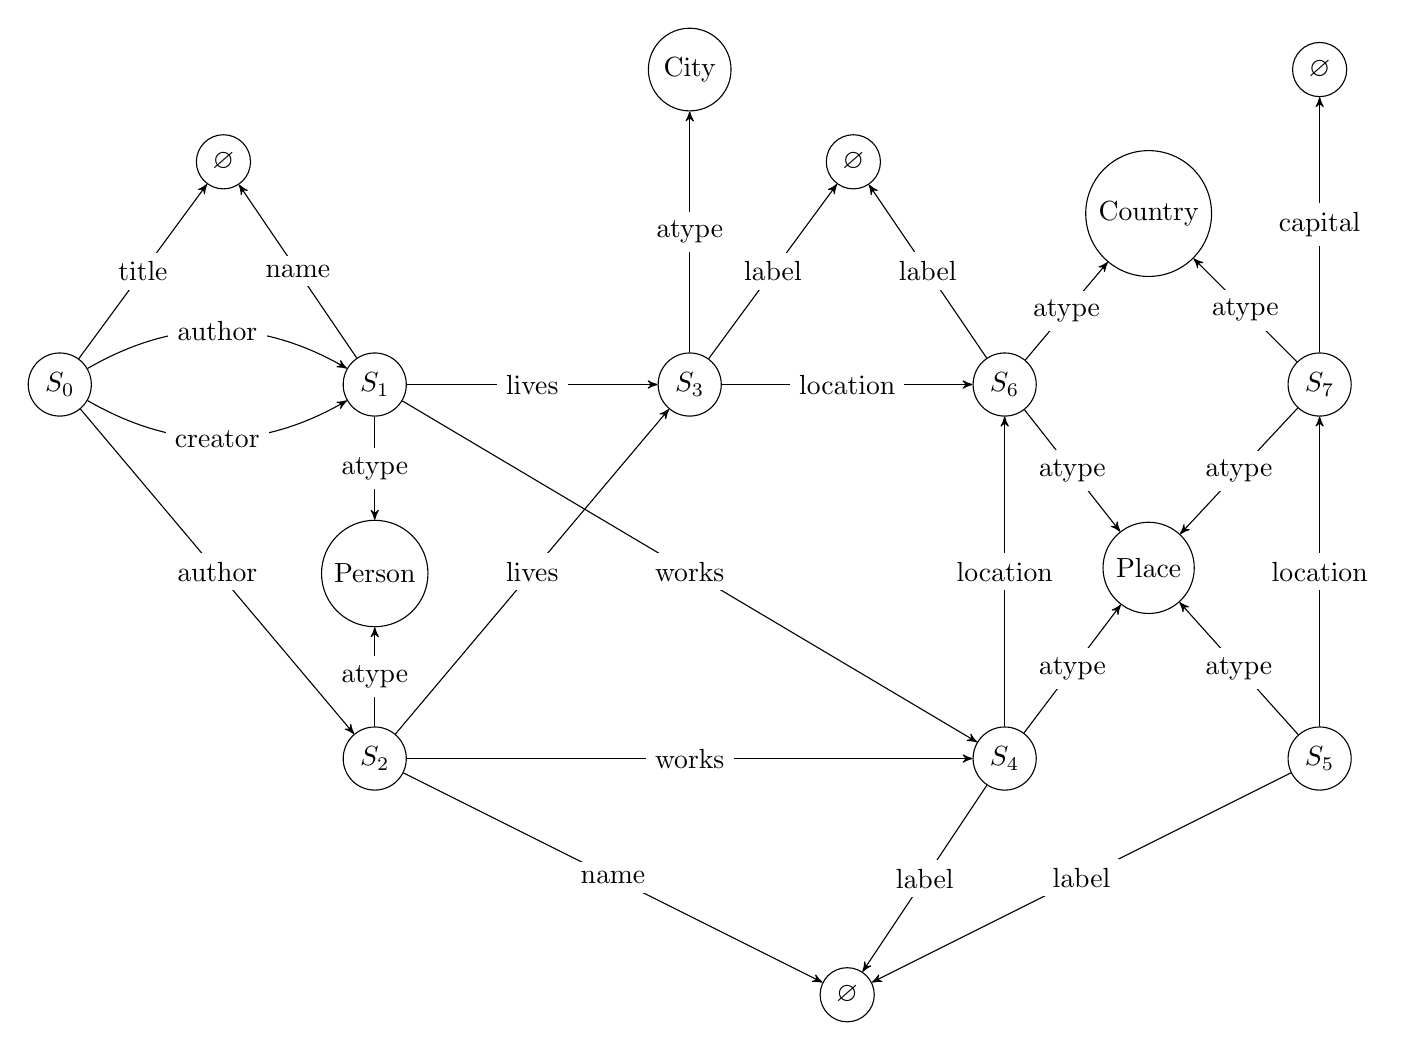
\begin{tikzpicture}[->,>=stealth',node distance=4cm]

\node [draw,circle] (n0) {$S_0$};
\node [draw,circle,right of = n0] (n1) {$S_1$};
\node [draw,circle,below of = n1,yshift=-.75cm] (n2) {$S_2$};
\node [draw,circle,right of = n1] (n3) {$S_3$};
\node [draw,circle,right of = n3] (n6) {$S_6$};
\node [draw,circle,below of = n6,yshift=-.75cm] (n4) {$S_4$};
\node [draw,circle,right of = n6] (n7) {$S_7$};
\node [draw,circle,right of = n4] (n5) {$S_5$};

\node [draw,circle,above of = n3] (city) {City};
\node [draw,circle,below right of = n6,xshift=-1cm,yshift=.5cm] (place) {Place};
\node [draw,circle,above of = place,yshift=.5cm] (country) {Country};
\node [draw,circle,above of = n2,yshift=-1.65cm] (person) {Person};

\node [draw,circle,above right of = n0,xshift=-.75cm] (s1) {$\varnothing$};
\node [draw,circle,above right of = n3,xshift=-.75cm] (s2) {$\varnothing$};
\node [draw,circle,below of = n4,yshift=1cm,xshift=-2cm] (s3) {$\varnothing$};
\node [draw,circle,above of = n7] (s4) {$\varnothing$};

\path
(n0) edge[bend right] node[fill=white] {creator} (n1)
(n0) edge[bend left] node[fill=white] {author} (n1)
(n0) edge node[fill=white] {author} (n2)
(n1) edge node[fill=white] {lives} (n3)
(n1) edge node[fill=white] {works} (n4)
(n2) edge node[fill=white] {lives} (n3)
(n2) edge node[fill=white] {works} (n4)
(n3) edge node[fill=white] {location} (n6)
(n4) edge node[fill=white] {location} (n6)
(n5) edge node[fill=white] {location} (n7)
(n4) edge node[fill=white] {\gls{atype}} (place)
(n5) edge node[fill=white] {\gls{atype}} (place)
(n6) edge node[fill=white] {\gls{atype}} (place)
(n7) edge node[fill=white] {\gls{atype}} (place)
(n6) edge node[fill=white] {\gls{atype}} (country)
(n7) edge node[fill=white] {\gls{atype}} (country)
(n1) edge node[fill=white] {\gls{atype}} (person)
(n2) edge node[fill=white] {\gls{atype}} (person)
(n3) edge node[fill=white] {\gls{atype}} (city)
(n0) edge node[fill=white] {title} (s1)
(n1) edge node[fill=white] {name} (s1)
(n3) edge node[fill=white] {label} (s2)
(n6) edge node[fill=white] {label} (s2)
(n2) edge node[fill=white] {name} (s3)
(n4) edge node[fill=white] {label} (s3)
(n5) edge node[fill=white] {label} (s3)
(n7) edge node[fill=white] {capital} (s4)
;
\end{tikzpicture}
		}
	\end{minipage}
	\quad
	\begin{minipage}[h]{.2\textwidth}
		\centering
		\caption*{$R_{fbt}\left(V, \mathcal{W}\right)$}
		\begin{tabular}{lc@{\hs}l}
			\toprule
			$V$ & \phantom{a} & $\mathcal{W}$ \\
			\cmidrule{1-1} \cmidrule{3-3}
			$N_0$ & \phantom{a} & $S_0$ \\
			$N_1$ & \phantom{a} & $S_1$ \\
			$N_2$ & \phantom{a} & $S_2$ \\
			$N_3$ & \phantom{a} & $S_3$ \\
			$N_4$ & \phantom{a} & $S_4$ \\
			$N_5$ & \phantom{a} & $S_5$ \\
			$N_6$ & \phantom{a} & $S_6$ \\
			$N_7$ & \phantom{a} & $S_7$ \\
			\bottomrule
		\end{tabular}
	\end{minipage}
	\caption{Summary of the graph in Figure~\ref{fig:graph} with bisimulation $R_{fbt}$ as the summarisation relation. The table indicates the mappings by $R_{fbt}$. The content in $G$ is abstracted by the sumnode $\varnothing$.}
	\label{fig:fbb-summary}
\end{figure}

\subsection{Approximate Graph Summary}
\label{sec:approximate}

%A graph summary is built so that it describes the structure of the graph, providing similar benefits as a relational schema does for a database, which we discuss in Section~\ref{chap03:sec:gschema}.
In general, we find in Web Data a heterogeneous use of vocabularies, where several different ontologies can be used within the same dataset, in ways that might not have been intended for. Web Data presents a complex graph structure that varies greatly from dataset to dataset.

In addition, Web Data is composed of user-created content which quality is not assessed, e.g., use of an appropriate ontology, typographic errors when editing, incorrect description of an entity, etc. This quality issue, combined with the heterogeneity of the graph, is an obstacle towards the generation of a precise summary. Indeed, attempting to record every single path would require a summary so large that its benefits would be nullified. Therefore, we present in this section \emph{approximate} graph summaries.

\subsubsection{Heterogeneous Graph Structure}

We investigate the direction of \emph{approximate} summarisation for the creation of a graph summary. DataGuides~\cite{goldman1997dataguides} were proposed to index the structure of data following the OEM model.
%A requirement of the approach is that every path in the DataGuide appears in the original graph as well.
The creation of a DataGuide is equivalent to the conversion of a non-deterministic finite automaton to a deterministic finite automaton.
Due to heterogeneous structure of the data, the size of a DataGuide grows exponentially, becoming larger than the original data as noted by Goldman et al.~\cite{goldman1999approximate}.

We created in~\cite{campinas:2011:eos} a dataset based on Sindice\footnote{\url{http://sindice.com}}'s collection for the task of entity-oriented search. The Figure~\ref{fig:onto-dist} depicts the distribution of the frequency of ontologies used across documents, i.e., the probability for an ontology to be used in exactly $n$ documents. The distribution shows a power-law distribution following a Zipf function with a slope of $\alpha = 2.27$.
%For example, one ontology (\url{http://purl.org/dc/terms/}) is used in more than 150 million documents and another one (\url{http://www.w3.org/2006/vcard/ns\#}) is used in more than 64 millions documents.

This investigation has showed that most ontologies (99\%) are used only once. However, the distribution tail is sparse, suggesting that a few ontologies are used in a large proportion of documents.
This result strengthens our belief that it is not a viable option in many cases for a graph summary to retain every path and combinations of paths that occur in an entity graph.

\begin{figure}
	\centering
	\input{04-summary/experiments/ontology-distribution}
	\caption{Ontology probability distribution}
	\label{fig:onto-dist}
\end{figure}

%\begin{itemize}
%\item Scalability issues (computation performance + summary size) of current graph summarisation
%\item Approximate definition of graph summarisation.
%\end{itemize}

\subsubsection{Approximate Summarisation Relation}

A graph summary can be constructed based on various features of the data. We present here some summarisation relations that consider the following features of the graph:
\begin{itemize}
	\item the predicate URI;
	\item the type URI; and
	\item the direction of links, i.e., incoming or outgoing.
\end{itemize}
We report in Table~\ref{tab:sumrel} the relations along with the name of the summary that it generates.

\begin{labeling}{$R_{ioat}$ \textbf{relation.}}
\item[$R_{st}$ \textbf{relation.}]

We define $R_{st}$ as the summarisation relation that maps a node according to its type. Formally:
$$
\begin{aligned}
R_{st} = \{ (u, x) \in V \times \mathcal{W}_{st} \mid &\; \exists (v,y) \in V \times \mathcal{W}_{st} \\
 & (u,\gls{atype},v) \in A \wedge (x,\gls{atype},y) \wedge l_V(v) = l_\mathcal{W}(y) \}
\end{aligned}
$$
The nodes $N_4$, $N_5$, $N_6$, and $N_7$ in the Figure~\ref{fig:graph} are mapped to a same sumnode since they all have \emph{Place} as a type. The $R_{st}$ relation may map a node to multiple sumnodes since an entity may have several types. For instance, the nodes $N_6$ and $N_7$ are also mapped to another sumnode since they both share the type \emph{Country}.

\item[$R_t$ \textbf{relation.}]

We define $R_t$ the relation that maps a node based on its set of types. Formally:
$$
R_t = \left\lbrace (u, x) \in V \times \mathcal{W}_t \mid types(u) = types(x) \right\rbrace
$$
The Figure~\ref{fig:classes-summary} depicts the $R_t$ summary of the graph in in the Figure~\ref{fig:graph}. The nodes $N_6$ and $N_7$ are mapped to the sumnode $S_4$ because they are both associated with the types \emph{Place} and \emph{Country}. The table indicates the mappings by $R_t$ of the nodes in $V$, e.g., the nodes $N_1$ and $N_2$ are mapped to the sumnode $S_1$ since both connect to $Person$ via the type attribute. It differs from $R_{st}$ since it considers the types of a node as \emph{set} rather than individually. Indeed, the node $N_6$ is mapped to two sumnodes under the relation $R_{st}$.

\item[$R_a$ \textbf{relation.}]

We define $R_a$ the relation that maps a node based on its set of predicates. Formally:
$$
R_a = \left\lbrace (u, x) \in V \times \mathcal{W}_a \mid attributes(u) = attributes(x) \right\rbrace
$$
The nodes $N_3$, $N_4$, and $N_5$ are $\sim_a$-equivalent because they share the same set of attributes, i.e., $\left\lbrace label, location, type \right\rbrace$. The graph in Figure~\ref{fig:attributes-summary} is the $\sim_a$-summary of the data graph in Figure~\ref{fig:graph}.

\begin{figure}
	\centering
	\begin{minipage}{.75\textwidth}
		\resizebox{\textwidth}{!}{
			\usetikzlibrary{arrows}

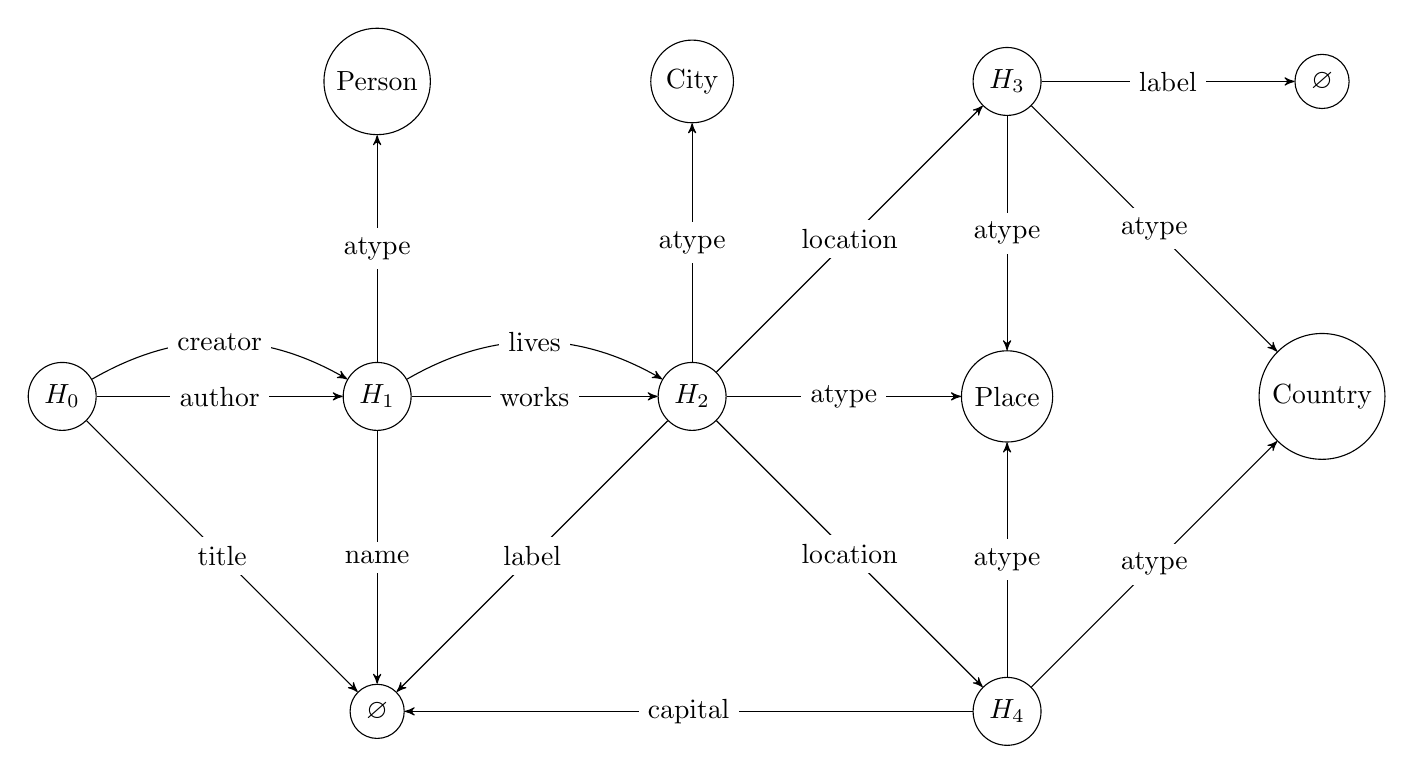
\begin{tikzpicture}[->,>=stealth',node distance=4cm]
\node [draw,circle] (n0) {$H_0$};
% \node (n0) [draw,thick,rectangle,inner sep=0] {
% \begin{tabular}{l}
% \multicolumn{1}{c}{$H_0$} \\
% \hline
% \\
% \hline
% - title
% \end{tabular}
% };

\node [draw,circle,right of = n0] (n1) {$H_1$};
% \node (n1) [draw,thick,rectangle,inner sep=0,right of = n0] {
% \begin{tabular}{l}
% \multicolumn{1}{c}{$H_1$} \\
% \hline
% - Person \\
% \hline
% - name
% \end{tabular}
% };

\node [draw,circle,above of = n1] (person) {Person};
\node [draw,circle,right of = n1] (n2) {$H_2$};
% \node (n2) [draw,thick,rectangle,inner sep=0,right of = n1] {
% \begin{tabular}{l}
% \multicolumn{1}{c}{$H_2$} \\
% \hline
% - City \\
% \hline
% - label
% \end{tabular}
% };

\node [draw,circle,right of = n2] (place) {Place};
\node [draw,circle,above of = place] (n3) {$H_3$};
% \node (n3) [draw,thick,rectangle,inner sep=0,above right of = n2] {
% \begin{tabular}{l}
% \multicolumn{1}{c}{$H_3$} \\
% \hline
% - Place \\
% - Country \\
% \hline
% - label
% \end{tabular}
% };

\node [draw,circle,above of = n2] (city) {City};
\node [draw,circle,below of = place] (n4) {$H_4$};
% \node (n4) [draw,thick,rectangle,inner sep=0,below right of = n2] {
% \begin{tabular}{l}
% \multicolumn{1}{c}{$H_4$} \\
% \hline
% - Place \\
% - Country \\
% \hline
% - capital
% \end{tabular}
% };

\node [draw,circle,right of = place] (country) {Country};
\node [draw,circle,below of = n1] (s1) {$\varnothing$};
\node [draw,circle,right of = n3] (s2) {$\varnothing$};

\path
(n0) edge node[fill=white] {author} (n1)
(n0) edge[bend left] node[fill=white] {creator} (n1)
(n1) edge node[fill=white] {\gls{atype}} (person)
(n1) edge node[fill=white] {works} (n2)
(n1) edge[bend left] node[fill=white] {lives} (n2)
(n2) edge node[fill=white] {\gls{atype}} (city)
(n2) edge node[fill=white] {location} (n3)
(n2) edge node[fill=white] {location} (n4)
(n2) edge node[fill=white] {\gls{atype}} (place)
(n3) edge node[fill=white] {\gls{atype}} (country)
(n4) edge node[fill=white] {\gls{atype}} (country)
(n3) edge node[fill=white] {\gls{atype}} (place)
(n4) edge node[fill=white] {\gls{atype}} (place)
(n0) edge node[fill=white] {title} (s1)
(n1) edge node[fill=white] {name} (s1)
(n2) edge node[fill=white] {label} (s1)
(n4) edge node[fill=white] {capital} (s1)
(n3) edge node[fill=white] {label} (s2)
;
\end{tikzpicture}
		}
	\end{minipage}
	\quad
	\begin{minipage}[h]{.2\textwidth}
		\centering
		\caption*{$R_a\left(V, \mathcal{W}\right)$}
		\resizebox{\textwidth}{!}{
		\begin{tabular}{lc@{\hs}l}
			\toprule
			$V$ & \phantom{a} & $\mathcal{W}$ \\
			\cmidrule{1-1} \cmidrule{3-3}
			$N_0$ & \phantom{a} & $S_0$ \\
			$N_1$, $N_2$ & \phantom{a} & $S_1$ \\
			$N_3$, $N_4$, $N_5$ & \phantom{a} & $S_2$ \\
			$N_6$ & \phantom{a} & $S_3$ \\
			$N_7$ & \phantom{a} & $S_4$ \\
			\bottomrule
		\end{tabular}}
	\end{minipage}
	\caption{Summary of the graph in Figure~\ref{fig:graph} with $R_a$. The table indicates the mappings by $R_a$. The content in $G$ is abstracted by the sumnode $\varnothing$.}
	\label{fig:attributes-summary}
\end{figure}

\item[$R_{at}$ \textbf{relation.}]

We define $R_{at}$ as the relation that maps a node based on its set of types and attributes. Formally:
$$
\begin{aligned}
R_{at} = \{ (u, x) \in V \times \mathcal{W}_{at} \mid &\; types(u) = types(x) \\
& \wedge attributes(u) = attributes(x) \}
\end{aligned}
$$
The nodes $N_1$ and $N_2$ are mapped to mapped to a same sumnode by $R_{at}$ because they are associated with the same type, i.e., \emph{Person}, and they have the same attributes, i.e., $\left\lbrace lives, name, type, works \right\rbrace$.

\item[$R_{ioa}$ \textbf{relation.}]

We define $R_{ioa}$ the relation based on the set of incoming and outgoing attributes; that is:
$$
\begin{aligned}
R_{ioa} =
\{
(u, x) \in V \times \mathcal{W}_{ioa} \mid &\; attributes(u) = attributes(x) \\
& \wedge attributes^{-1}(u) = attributes^{-1}(x)
\}
\end{aligned}
$$
All three nodes $N_3$, $N_4$, and $N_5$ map to the same sumnode by the relation $R_a$. However with $R_{ioa}$, each is assigned to a separate sumnode, since all three have different incoming set of attributes, i.e., $\left\lbrace lives \right\rbrace$, $\left\lbrace works \right\rbrace$, and $\varnothing$, respectively.

\item[$R_{ia}$ \textbf{relation.}]

We define $R_{ia}$ as the relation based on the set of incoming attributes; that is:
\begin{equation*}
R_{ia} = \left\lbrace (u, x) \in V \times \mathcal{W}_{ia} \mid attributes^{-1}(u) = attributes^{-1}(x) \right\rbrace
\end{equation*}

\item[$R_{iat}$ \textbf{relation.}]

We define $R_{iat}$ as the relation based on the set of types and incoming attributes; that is:
$$
\begin{aligned}
R_{iat} = \{ (u, x) \in V \times \mathcal{W}_{iat} \mid &\; types(u) = types(x) \\
& \wedge attributes^{-1}(u) = attributes^{-1}(x) \}
\end{aligned}
$$

\item[$R_{ioat}$ \textbf{relation.}]

The relation $R_{ioat}$ maps a node based on the set of types, and the incoming and outgoing attributes sets. Formally, it is defined as:
$$
\begin{aligned}
R_{ioat} = \{ (u, x) \in V \times \mathcal{W}_{ioat} \mid &\; types(u) = types(x) \\
& \wedge attributes(u) = attributes(x) \\
& \wedge attributes^{-1}(u) = attributes^{-1}(x) \}
\end{aligned}
$$
Although the nodes $N_1$ and $N_2$ are mapped to a same sumnode with $R_{at}$, that is not the case with the relation $R_{ioat}$, because only the node $N_2$ has the incoming attribute $creator$.
% With $R_{ioa}$ and $R_{ioat}$, the incoming set of attributes is computed by reversing the direction of edges, i.e., the target becomes the source, and then grouping on the source node.
%For these relations, the complexity is equal to $O\left(\vert A \vert\right)$, since we need to visit each edge in order to assign the node at the source of an edge to an equivalence class.
\end{labeling}

\begin{table}
	\centering
	\resizebox{\textwidth}{!}{
	\begin{tabular}{lc@{\hs}lc@{\hs}l}
	\toprule
	 & \phantom{a} & \multicolumn{1}{c}{Notation} & \phantom{a} & \multicolumn{1}{c}{Summarisation Relation} \\
	\cmidrule{3-3} \cmidrule{5-5}
	\emph{Single Type} & \phantom{a} & $\mathcal{S}_{st} = \left\langle \mathcal{W}_{st}, \mathcal{B}_{st}, l_{\mathcal{W}_{st}} \right\rangle$ & \phantom{a} & $R_{st} = \left\lbrace (u, x) \in V \times \mathcal{W}_{st} \mid \exists (u, \gls{atype}, t) \in A : x \leftrightsquigarrow t \right\rbrace$ \\
	\emph{Types} & \phantom{a} & $\mathcal{S}_t = \left\langle \mathcal{W}_t, \mathcal{B}_t, l_{\mathcal{W}_t} \right\rangle$ & \phantom{a} & $R_t = \left\lbrace (u, x) \in V \times \mathcal{W}_t \mid x \leftrightsquigarrow types(u) \right\rbrace$ \\
	\emph{Attributes} & \phantom{a} & $\mathcal{S}_a = \left\langle \mathcal{W}_a, \mathcal{B}_a, l_{\mathcal{W}_a} \right\rangle$ & \phantom{a} & $R_a = \left\lbrace (u, x) \in V \times \mathcal{W}_a \mid x \leftrightsquigarrow attributes(u) \right\rbrace$ \\
	\emph{Attributes \& Types} & \phantom{a} & $\mathcal{S}_{at} = \left\langle \mathcal{W}_{at}, \mathcal{B}_{at}, l_{\mathcal{W}_{at}} \right\rangle$ & \phantom{a} & $R_{at} = \left\lbrace (u, x) \in V \times \mathcal{W}_{at} \mid x \leftrightsquigarrow types(u) \cup attributes(u) \right\rbrace$ \\
	\emph{IO Attributes} & \phantom{a} & $\mathcal{S}_{ioa} = \left\langle \mathcal{W}_{ioa}, \mathcal{B}_{ioa}, l_{\mathcal{W}_{ioa}} \right\rangle$ & \phantom{a} & $R_{ioa} = \left\lbrace (u, x) \in V \times \mathcal{W}_{ioa} \mid x \leftrightsquigarrow attributes(u) \cup attributes^{-1}(u) \right\rbrace$ \\
	\emph{IO Attributes \& Types} & \phantom{a} & $\mathcal{S}_{ioat} = \left\langle \mathcal{W}_{ioat}, \mathcal{B}_{ioat}, l_{\mathcal{W}_{ioat}} \right\rangle$ & \phantom{a} & $R_{ioat} = \left\lbrace (u, x) \in V \times \mathcal{W}_{ioat} \mid x \leftrightsquigarrow types(u) \cup attributes(u) \cup attributes^{-1}(u) \right\rbrace$ \\
	\bottomrule
	\end{tabular}}
	\caption{Summarisation relations}
	\label{tab:sumrel}
\end{table}


\section{Graph Summary Generation}
\label{chap:summary:algo}

In this section, we present an algorithm for generating a graph summary. Some optimisations are possible depending on the relation. However, the proposed approach is independent of the summarisation relation used in order to cater for most relations. The algorithm takes a graph in input and outputs a graph summary, which is distinct from the input graph.
We first present a version of the algorithm for a single dataset and then for a collection of several.
Next, we describe two implementations of the algorithm, one based on MapReduce~\cite{dean:2004:msd}, and the other on SPARQL.

\subsection{Algorithm}

The creation of a graph summary is decomposed into three steps. In a first step, we aggregate all the information about a node needed for the summarisation relation. In a second step, we create a table that associates an entity (a node of $G$) to a sumnode. In a third step, we materialise the sumedges by joining the previous table with the original graph.

\subsubsection{Graph Summarisation of a Single Dataset}

We present here the graph summarisation algorithm that is aimed at processing a single dataset.
%The Figure~\ref{fig:gs-algo} depicts the overall algorithm for generating a graph summary.
The Algorithm~\ref{alg:summary} outlines the flow of the graph summarisation which takes a graph as input and outputs its summary. For each edge of the graph, the algorithm first retrieves the sumnodes corresponding to the source and target nodes thanks to the \texttt{GetSumnode} function. Then, the corresponding sumedge is added to the summary. The lines~2-5 represent the first two steps of the graph summary creation, and the line~7 corresponds to the materialisation of the sumedge.

\begin{remark}
On line~5 we retrieve the sumnode of $v$ only if it is not a type, since we consider the type as a feature of the summarisation relation.
\end{remark}

%\begin{figure}
%	\centering
%	\usetikzlibrary{shapes,arrows}

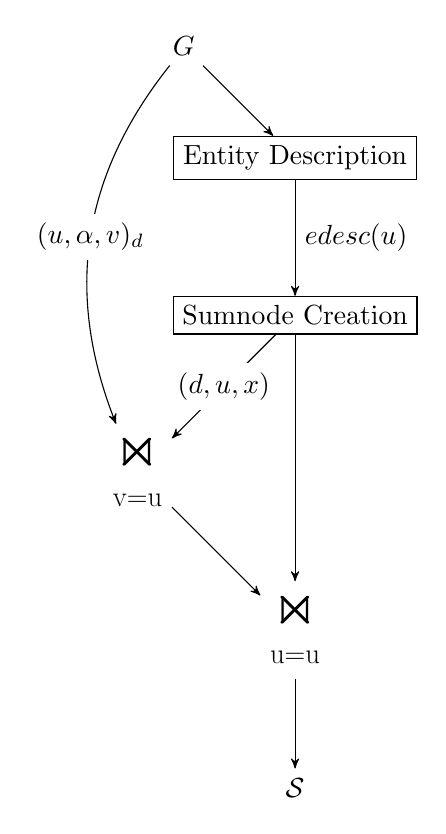
\begin{tikzpicture}[->,>=stealth',node distance=2cm]
\node (1) {$G$};
\node[draw,below right of = 1] (2) {Entity Description};
\node[draw,below of = 2] (3) {Sumnode Creation};
\node[below of = 3,xshift=-2cm] (4) {{\huge $\underset{\scalebox{0.5}{v=u}}{\Join}$}};
\node[below of = 4,xshift=2cm] (5) {{\huge $\underset{\scalebox{0.5}{u=u}}{\Join}$}};
\node[below of = 5] (6) {$\mathcal{S}$};

\path
(1) edge (2)
(2) edge node[right] {$\glssymbol{edesc}(u)$} (3)
(1) edge[bend right]  node[fill=white] {$(u, \alpha, v)_d$} (4)
(3) edge node[fill=white] {$(d,u,x)$} (4)
(3) edge (5)
(4) edge (5)
(5) edge (6)
;
\end{tikzpicture}
%	\caption{Graph summarisation flow. $(u, \alpha, v) \in A$ is an edge of $G$, $(d, u, x) \in D \times V \times \mathcal{V}$ is a tuple associating a node $u$ to a sumnode $x$ within a dataset $d$. We use the summarisation relation only within the ``Sumnode Creation'' step.}
%	\label{fig:gs-algo}
%\end{figure}

\begin{algorithm}
	\DontPrintSemicolon
	\SetKwFunction{sn}{GetSumnode}
	\KwIn{A graph $G=\left\langle V, A, l_V \right\rangle$}
	\KwOut{A summary $\mathcal{S}=\left\langle \mathcal{V}, \mathcal{A}, l_\mathcal{V} \right\rangle$ of $G$}
	\BlankLine
	\ForEach{$(u, \alpha, v) \in A$}{
		\tcp{Sumnode of the source node $u$}
		$S_u \gets \sn(u)$ \;
		\tcp{Sumnode of the target node $v$}
		$S_v \gets \varnothing$ \;
		\If(\tcp*[h]{$\alpha$ is not an attribute type}){$\alpha \not \in \mathcal{L}^T$}{
			$S_v \gets \sn(v)$ \;
		}
		\tcp{Build the graph summary}
		$\mathcal{V} \gets \mathcal{V} \cup \{ S_u, S_v \}$ \;
		$\mathcal{A} \gets \mathcal{A} \cup \{ (S_u, \alpha, S_v) \}$ \;
	}
	\caption{Graph summarisation of a single dataset}
	\label{alg:summary}
\end{algorithm}

\begin{labeling}{\textbf{\underline{Step 2:}} \emph{Node to sumnode mapping.}}
\item[\textbf{\underline{Step 1:}} \emph{Entity description.}]
\phantomsection
\label{step-ed}
In order to create a graph summary, the basic information we manipulate is an entity. The computation of the entity description \gls{edesc} requires a pass over the edges, with a worst case complexity of $O(\vert A \vert)$. The entity description provides the necessary contextual information needed for the summarisation relation.

\item[\textbf{\underline{Step 2:}} \emph{Node to sumnode mapping.}]
\phantomsection
\label{step-hn}
A sumnode unique identifier is defined based on the entity description \gls{edesc}, with regards to the summarisation relation. This is the core operation of the \texttt{GetSumnode} function, which assigns a sumnode to a node. For example, a unique identifier can be created from the types of an entity for the relation $R_t$.
The worst case complexity of this operation is $O(\vert V \vert)$, since we need to visit each node of the graph.

\item[\textbf{\underline{Step 3:}} \emph{Sumedge materialisation.}]
\phantomsection
\label{step-he}
We need to join the previous mappings of node to sumnode with the original graph in order to materialise an sumedge. We do this by two joins, i.e., on the source and target nodes. In this step, we need to visit each edge in the graph, so in the worst case it has a $O\left(\vert A \vert\right)$ complexity.

\item[\textbf{\underline{Step 4:}} \emph{Statistics gathering.}]
\phantomsection
\label{step-stats}
During the previous steps, it is possible to gather statistics about the graph. In the Step~2, we can keep the count of nodes that are mapped to a sumnode. In the Step~3, we can count the occurrences of an edge between two sumnodes. Such statistics provide insight into the graph structure, complementing the graph summary.
\end{labeling}

\paragraph{Example.}

In the Figure~\ref{tab:algo-ex}, we depict the \emph{Types} summarisation $R_t$ of a graph describing people and documents. In Step~2 we assign the sumnode \emph{h1} to the nodes (i.e., \emph{:e1} and \emph{:e3}) of type \emph{:Person}, and \emph{h2} to the node (i.e., \emph{:e2}) of type \emph{:Document}. In Step~3, we join the edges of the input graph with the table created in Step~2 in order to retrieve the sumnodes.
It is possible to gather statistics about the summarisation by, e.g., grouping over the sumnodes and counting the number of rows in a group. The Figure~\ref{fig:algo-ex} depicts the \emph{Types} summary that is outputted in the Figure~\ref{tab:algo-ex}.

\begin{figure}
	\centering
	\begin{subfigure}{\textwidth}
		\centering
		\resizebox{\textwidth}{!}{
			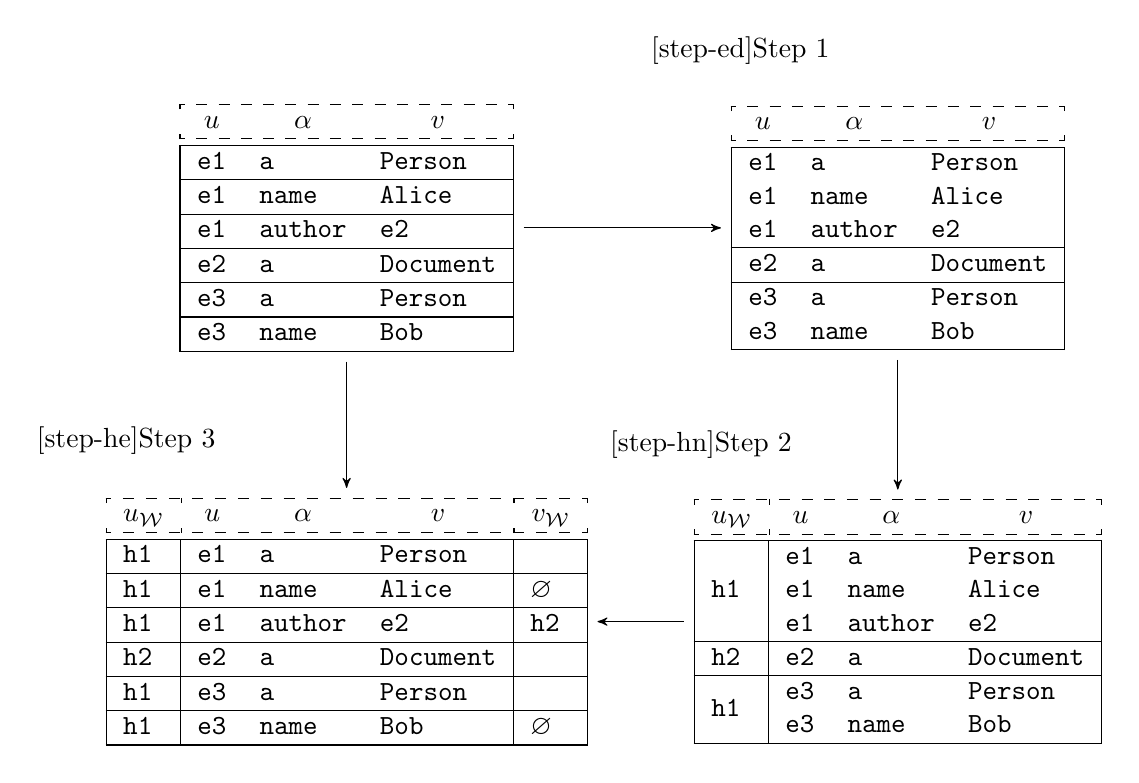
\begin{tikzpicture}[->,>=stealth',node distance=5cm]
\node (data) {
\begin{tabular}{|lll|}
\hdashline
\multicolumn{1}{:c}{$u$} & \multicolumn{1}{c}{$\alpha$} & \multicolumn{1}{c:}{$v$} \\
\hdashline
\hline
\texttt{e1} & \texttt{a} & \texttt{Person} \\
\hline
\texttt{e1} & \texttt{name} & \texttt{Alice} \\
\hline
\texttt{e1} & \texttt{author} & \texttt{e2} \\
\hline
\texttt{e2} & \texttt{a} & \texttt{Document} \\
\hline
\texttt{e3} & \texttt{a} & \texttt{Person} \\
\hline
\texttt{e3} & \texttt{name} &  \texttt{Bob} \\
\hline
\end{tabular}
};

\node[right of = data,xshift=2cm] (edesc) {
\begin{tabular}{|lll|}
\hdashline
\multicolumn{1}{:c}{$u$} & \multicolumn{1}{c}{$\alpha$} & \multicolumn{1}{c:}{$v$} \\
\hdashline
\hline
\texttt{e1} & \texttt{a} & \texttt{Person} \\
\texttt{e1} & \texttt{name} & \texttt{Alice} \\
\texttt{e1} & \texttt{author} & \texttt{e2} \\
\hline
\texttt{e2} & \texttt{a} & \texttt{Document} \\
\hline
\texttt{e3} & \texttt{a} & \texttt{Person} \\
\texttt{e3} & \texttt{name} &  \texttt{Bob} \\
\hline
\end{tabular}
};

\node[below of = edesc] (gsv) {
\begin{tabular}{|l|lll|}
\hdashline
\multicolumn{1}{:c}{$u_\mathcal{W}$} & \multicolumn{1}{:c}{$u$} & \multicolumn{1}{c}{$\alpha$} & \multicolumn{1}{c:}{$v$} \\
\hdashline
\hline
\texttt{\multirow{3}{*}{h1}} & \texttt{e1} & \texttt{a} & \texttt{Person} \\
& \texttt{e1} & \texttt{name} & \texttt{Alice} \\
& \texttt{e1} & \texttt{author} & \texttt{e2} \\
\hline
\texttt{h2} & \texttt{e2} & \texttt{a} & \texttt{Document} \\
\hline
\texttt{\multirow{2}{*}{h1}} & \texttt{e3} & \texttt{a} & \texttt{Person} \\
& \texttt{e3} & \texttt{name} &  \texttt{Bob} \\
\hline
\end{tabular}
};

\node[below of = data] (join2) {
\begin{tabular}{|l|lll|l|}
\hdashline
\multicolumn{1}{:c}{$u_\mathcal{W}$} & \multicolumn{1}{:c}{$u$} & \multicolumn{1}{c}{$\alpha$} & \multicolumn{1}{c:}{$v$} & \multicolumn{1}{:c:}{$v_\mathcal{W}$} \\
\hdashline
\hline
\texttt{h1} & \texttt{e1} & \texttt{a} & \texttt{Person} & \\
\hline
\texttt{h1} & \texttt{e1} & \texttt{name} & \texttt{Alice} & \texttt{$\varnothing$} \\
\hline
\texttt{h1} & \texttt{e1} & \texttt{author} & \texttt{e2} & \texttt{h2} \\
\hline
\texttt{h2} & \texttt{e2} & \texttt{a} & \texttt{Document} & \\
\hline
\texttt{h1} & \texttt{e3} & \texttt{a} & \texttt{Person} & \\
\hline
\texttt{h1} & \texttt{e3} & \texttt{name} &  \texttt{Bob} & \texttt{$\varnothing$} \\
\hline
\end{tabular}
};

\node at ($ (edesc) + (-2,2.25) $) {\hyperref[step-ed]{Step 1}};
\node at ($ (gsv) + (-2.5,2.25) $) {\hyperref[step-hn]{Step 2}};
\node at ($ (join2) + (-2.8,2.3) $) {\hyperref[step-he]{Step 3}};

%  \coordinate (p1x) at ($ (join2) + (-3.6,2) $);
%  \coordinate (p1y) at ($ (join2) + (3.6,-2) $);
%  \draw[rounded corners,dotted]  (p1x) node[yshift=.3cm] {\hyperref[step-he]{Step 3}} rectangle (p1y);
%
%  \coordinate (p2x) at ($ (edesc) + (-2.8,1.95) $);
%  \coordinate (p2y) at ($ (edesc) + (2.8,-1.95) $);
%  \draw[rounded corners,dotted]  (p2x) node[yshift=.3cm] {\hyperref[step-ed]{Step 1}} rectangle (p2y);
%
%  \coordinate (p3x) at ($ (gsv) + (-3.3,1.95) $);
%  \coordinate (p3y) at ($ (gsv) + (3.3,-1.95) $);
%  \draw[rounded corners,dotted]  (p3x) node[yshift=.3cm] {\hyperref[step-hn]{Step 2}} rectangle (p3y);

\path
(data) edge (edesc)
(data) edge (join2)
(edesc) edge (gsv)
% (gsv) edge[bend right=15] (join1sym)
% (join1) edge (join2sym)
(gsv) edge (join2)
;
\end{tikzpicture}

		}
		\caption{The input data is a set of edges, one per row. The columns $u_\mathcal{V}$ and $v_\mathcal{V}$ represents the sumnodes associated with the node $u$ and $v$, respectively. The Step~2 assigns the sumnode \emph{h1} to the nodes \emph{e1} and \emph{e3}; and the sumnode \emph{h2} to the node \emph{e3}. These sumnodes are joined with the input edges in Step~3 in order to materialise the sumedges.}
		\label{tab:algo-ex}
	\end{subfigure}
	\qquad
	\begin{subfigure}{.7\textwidth}
		\centering
		\resizebox{.7\textwidth}{!}{
			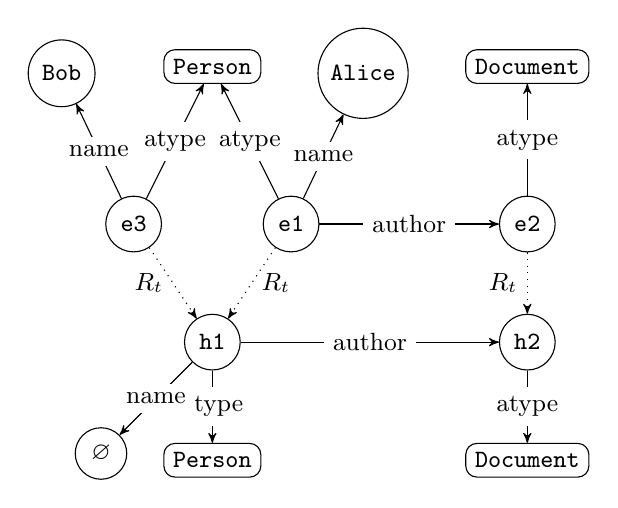
\begin{tikzpicture}[every node/.style={font=\ttfamily\small},main node/.style={draw,circle},type node/.style={rounded corners,draw},->,>=stealth',node distance=2cm]

\node[main node] (e1) {e1};
\node[main node,left of = e1] (e3) {e3};
\node[main node,right of = e1,xshift=1cm] (e2) {e2};

\node[main node,above right of = e1,xshift=-.5cm,yshift=.5cm] (alice) {Alice};
\node[main node,above left of = e3,xshift=.5cm,yshift=.5cm] (bob) {Bob};

\node[type node,above of = e1,xshift=-1cm] (person) {Person};
\node[type node,above of = e2] (doc) {Document};

\node[main node,below of = e1,xshift=-1cm,yshift=.5cm] (h1) {h1};
\node[main node,below of = e2,yshift=.5cm] (h2) {h2};

\node[type node,below of = h1,yshift=.5cm] (tperson) {Person};
\node[type node,below of = h2,yshift=.5cm] (tdoc) {Document};
\node[main node,below left of = h1] (not) {$\varnothing$};

\path[every node/.style={font=\small}]
(e1) edge node[fill=white] {\glssymbol{atype}} (person)
(e3) edge node[fill=white] {\glssymbol{atype}} (person)
(e2) edge node[fill=white] {\glssymbol{atype}} (doc)
(e1) edge node[fill=white] {author} (e2)
(e1) edge node[fill=white] {name} (alice)
(e3) edge node[fill=white] {name} (bob)

(e1) edge[dotted] node[right] {$R_t$} (h1)
(e2) edge[dotted] node[left] {$R_t$} (h2)
(e3) edge[dotted] node[left] {$R_t$} (h1)

(h1) edge node[fill=white] {\glssymbol{atype}} (tperson)
(h2) edge node[fill=white] {\glssymbol{atype}} (tdoc)
(h1) edge node[fill=white] {name} (not)
(h1) edge node[fill=white] {author} (h2)

;
\end{tikzpicture}
		}
		\caption{Depiction of the \emph{Types} summary created in Figure~\ref{tab:algo-ex}.}
		\label{fig:algo-ex}
	\end{subfigure}
	\caption{Example of the \emph{Types} summarisation $R_t$ in the case of a single dataset.}
\end{figure}

\subsubsection{Graph Summarisation of Inter-Linked Datasets}
\label{chap03:summary:impl:inter-datasets}

The Web Data is a collection of semi-structured data that hail from a variety of sources. Sources may provide overlapping information and reference each other. In such an environment, questions of trust about the legality of information arise, e.g.,, whether one has the permission to describe some entity (node in the graph). Since the graph summary is built from the data itself, it may report an unexpected structure of the graph in the case of inter-linked datasets, which is discussed in the next paragraph.

\paragraph{Danger of summarising heterogeneous inter-linked datasets.}

The information about an entity can be spread across several datasets. In the Web of Data this happens when a same entity URI is reused across datasets. The \hyperref[step-hn]{Step 2} of the graph summarisation relies on the entity description \gls{edesc} in order to create the corresponding sumnode. Some edges of the description might be erroneous, which would then impact negatively on the summary.

In Figure~\ref{fig:sum-issue} we depict the summarisation of a graph which edges are spread over the datasets \emph{D1} and \emph{D2}. The former contains the edges $\{ (N_1, a, Person), (N_1, name, John) \}$, while the latter contains $\{ (N_1, a, Fiction), (N_1, title, Rama) \}$. Since the same node $N_1$ is used in \emph{D1} and \emph{D2}, all four edges contribute to the summarisation relation. That node is then mapped to the sumnode $T_1$ according to the \emph{Types} summarisation relation $R_t$.
Due to the overlap over \emph{D1} and \emph{D2} of $N_1$'s entity description, the sumnode reports that it is of both types \emph{Person} and \emph{Fiction}, as well as both attributes \emph{name} and \emph{title}.

Therefore, information about an entity within a dataset can be erroneous, e.g., either the graph in \emph{D1} or in \emph{D2}, which leads to a misleading graph summary.
In order to prevent this issue, we need to differentiate edges within \emph{D1} from those in \emph{D2}.

\begin{figure}
	\centering
	\resizebox{.8\textwidth}{!}{
		\usetikzlibrary{arrows,calc}

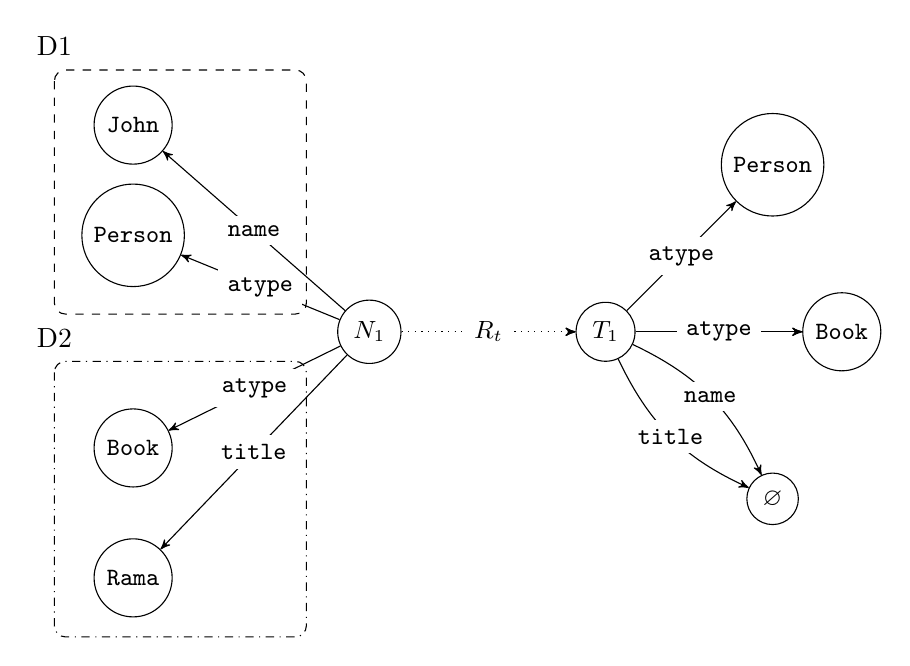
\begin{tikzpicture}[->,>=stealth',node distance=3cm,main node/.style={draw,circle,font=\small\ttfamily}]
\node (n1a) {};
\node[below of = n1a,yshift=-1cm] (n1b) {};

\node[main node,below of = n1a,yshift=1.125cm] (n1) {$N_1$};

\node[main node,left of = n1a,yshift=-.65cm] (person) {Person};
\node[main node,left of = n1b,yshift=.65cm] (doc) {Book};
\node[main node,left of = n1a,yshift=.75cm] (john) {John};
\node[main node,left of = n1b,yshift=-1cm] (rama) {Rama};

\coordinate (d1x) at ($ (person) + (-1,2.1) $);
\coordinate (d1y) at ($ (person) + (2.2,-1) $);
\draw[rounded corners,dashed]  (d1x) node[yshift=.3cm] {D1} rectangle (d1y);

\coordinate (d2x) at ($ (doc) + (-1,1.1) $);
\coordinate (d2y) at ($ (doc) + (2.2,-2.4) $);
\draw[rounded corners,dashdotted]  (d2x) node[yshift=.3cm] {D2} rectangle (d2y);

\node[main node,right of = n1] (t1) {$T_1$};
\node[main node,above right of = t1] (tperson) {Person};
\node[main node,right of = t1] (tdoc) {Book};
\node[main node,below right of = t1] (tvn) {$\varnothing$};

\path[every node/.style={fill=white,font=\small\ttfamily}]
(n1) edge node {\glssymbol{atype}} (person)
		edge node {name} (john)
		edge[dotted] node {$R_t$} (t1)
 edge node {\glssymbol{atype}} (doc)
		edge node {title} (rama)
		edge[dotted] node {$R_t$} (t1)
(t1) edge node {\glssymbol{atype}} (tperson)
		edge node {\glssymbol{atype}} (tdoc)
		edge node {\glssymbol{atype}} (tdoc)
		edge[bend left = 20] node {name} (tvn)
		edge[bend right = 20] node {title} (tvn)
;
\end{tikzpicture}
	}
	\caption{Heterogeneous data source issue with the \emph{Types} summarisation relation $R_t$}
	\label{fig:sum-issue}
\end{figure}

\paragraph{Edge authority.}

In this section, we introduce the concept of \emph{edge authority} which is needed for the summarisation of inter-linked datasets.

\begin{labeling}{\emph{Provenance:}}
	\item[\emph{Provenance:}] Due to the principle of Linked Data which states that anything can be said about anything, there is a need to know the provenance of an edge. This necessity goes in accordance with the N-Quads\footnote{\url{http://www.w3.org/TR/n-quads/}} serialisation format. The provenance of an edge indicates the dataset it is originally from.
	
	\item[\emph{Ownership:}] To assess the information given by an edge, we need to know the ownership of an entity (a node) in addition to the edge's provenance. This concept differs from the \emph{provenance} of an edge in the sense that a dataset may contain statements (edges) about an entity, but not necessarily owns that entity.
\end{labeling}

\begin{definition}[Edge Provenance]
	Let $G = \left\langle V, A, l_V \right\rangle$ be a graph. The provenance of an edge in $G$ is the dataset label of $G$, i.e., $\gls{Glabel}(G)$.
\end{definition}

\begin{definition}[Node Ownership]
	Let $G = \left\langle V, A, l_V \right\rangle$ be a graph and $\gls{D}$ the set of dataset labels. The ownership of a node is the function $\gls{dsource} : V \mapsto \gls{D}$ which maps a node to a dataset label.
\end{definition}

\begin{remark}
	In the case of inter-linked datasets, the provenance of edges that describe an entity may differ from the ownership of that entity.
\end{remark}

The authority of an edge combines the concepts of provenance and ownership, in order to determine whether that edge is ``legal'' or not. An edge is legal if the provenance of the edge is the same as the ownership of the source node.

\begin{definition}[Edge Authority]
	Let $G = \left\langle V, A, l_V \right\rangle$ be a graph.
	An edge $(u, \alpha, v) \in A$ of the graph $G$ has authority if $\gls{dsource}(u) = \gls{Glabel}(G)$.
\end{definition}

\begin{remark}
	In RDF, an edge which source node is a blank node has authority implicitly, since it is local to the dataset it originates from.
\end{remark}

The Figure~\ref{fig:authority} depicts various cases of authority. A dataset is represented by a colour and a line type, i.e., there are three datasets {\bfseries A}, {\bfseries B}, and {\bfseries C} which are dotted red, solid blue, and dashed green, respectively. The edges are coded in the same way, according to its provenance.

The provenance of the nodes $a_1$ and $a_2$ is dataset {\bfseries A}. The ownership of the node $b_1$ is dataset {\bfseries B}. Both edges (dotted and red edges) from $a_1$ to $a_2$ and $b_1$ have \emph{authority} since
\begin{inparaenum}[(1)]
	\item the ownership of the source node is dataset {\bfseries A}, i.e., $\gls{dsource}(a_1) = \textbf{A}$; and
	\item the provenance of both edges is dataset {\bfseries A}, i.e., $\gls{Glabel}(G_A) = \textbf{A}$ with $G_A$ the graph which dataset label is \textbf{A}.
\end{inparaenum}

The edge (solid and blue edge) from $a_2$ to $b_1$ has \textbf{no} authority, since its provenance is {\bfseries B} although it is about a node of {\bfseries A}. Similarly, the edge (dashed and green edge) from $a_1$ to $b_1$ has no authority either, since its provenance is not equal to the ownership of node $a_1$.

\begin{figure}
	\centering
	\usetikzlibrary{shapes,arrows}

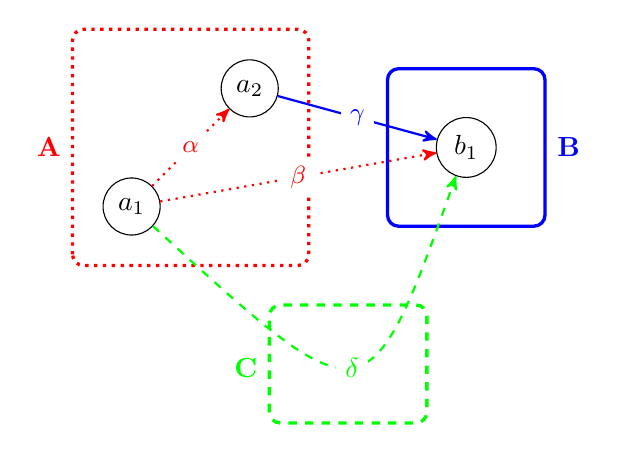
\begin{tikzpicture}[->,>=stealth']
\node [red] at (-1.3,.5) {{\bfseries A}};
\draw [red,dotted,rounded corners,very thick] (-1,-1) rectangle (2,2);
\node [draw,circle] (a1) at (-.25,-.25) {$a_1$};
\node [draw,circle] (a2) at (1.25,1.25) {$a_2$};

\node [blue] at (5.3,.5) {{\bfseries B}};
\draw [blue,rounded corners,very thick] (3,-.5) rectangle (5,1.5);
\node [draw,circle] (b1) at (4,.5) {$b_1$};

\node [green] at (1.2,-2.3) {{\bfseries C}};
\draw [green,dashed,rounded corners,very thick] (1.5,-3) rectangle (3.5,-1.5);

\path[every node/.style={fill=white,font=\small}]
 (a1) edge[red,thick,dotted] node {$\alpha$} (a2)
		  (a1) edge[red,thick,dotted] node {$\beta$} (b1)
		  (a2) edge[blue,thick] node {$\gamma$} (b1);
\draw [green,thick,dashed] (a1) .. controls (2.75,-3) .. node[fill=white] {$\delta$} (b1);
\end{tikzpicture}
	\caption{Edge authority. A dataset is represented by a colour and a line type. Edges are coded in the same way, based on the provenance of the edge.}
	\label{fig:authority}
\end{figure}

\paragraph{Algorithm.}

%Step2
%In order to compute the summary over a collection of datasets, we need to record the dataset label from where the entity description originates from. The output of this step is a list of tuples, i.e., $\left\lbrace (d, u, x) \in D \times V \times \mathcal{V} \right\rbrace$ where $d$ is a dataset label, $u$ a node and $x$ a sumnode. We remark that the sumnode is ``local'' to the dataset, since information about an entity can be scattered over several datasets.
%Step3
%Although this would duplicate some elements of the list of tuples, the various data sources for an entity forces it. This occurs whenever datasets link to each other.

In order to summarize a collection of inter-linked datasets, we extend the Algorithm~\ref{alg:summary} with the dataset label information.
%We augment the edges of the input graphs with their provenance.
%The Algorithm~\ref{alg:id-summary} modifies the function \texttt{GetSumnode} so to make it aware of the dataset label component.
The Algorithm~\ref{alg:id-summary} modifies the function \texttt{GetSumnode} so to implement the edge authority.
We name it as \texttt{GetSumnode\textsubscript{i}} to mark this change.
We extract the features for the summarisation relation from the edges in the entity description \gls{edesc} depending on two conditions:
\begin{enumerate}[topsep=0pt,itemsep=-1ex,partopsep=1ex,parsep=1ex]
\item the edge has authority; or
\item the provenance of the edge is $G_i$.
\end{enumerate}
By doing so, we retain the summarisation features from each dataset. This ensures we can summarise a dataset that reuses a node external to it, without corrupting the information about that node. The features which have authority are always used in order to support the case where a dataset reuses a node it didn't provide the necessary summarisation features for (e.g., types).

\begin{algorithm}
	\DontPrintSemicolon
	\SetKwProg{Fn}{Function}{:}{end}
	\SetKwFunction{sn}{GetSumnode\textsubscript{i}}
	\KwIn{A collection of $n$ graphs: $\forall 0 < i < n\; G_i=\left\langle V_i, A_i, l_{V_i} \right\rangle$. Let $G =\left\langle V, A, l_{V} \right\rangle$ be the union of all graphs, i.e., $A = A_1 \cup \cdots \cup A_n$ and $V = V_1 \cup \cdots \cup V_n$}
	\KwOut{A sumnode of the summary $\mathcal{S}=\left\langle \mathcal{V}, \mathcal{A}, l_\mathcal{V} \right\rangle$ of $G$}
	\BlankLine
%	\ForEach{$(u, \alpha, v)_i \in A$}{
%		\tcp{Sumnode of the source node $u$}
%		$S_u \gets \sn{u}$ \;
%		\tcp{Sumnode of the target node $v$}
%		$S_v \gets \varnothing$ \;
%		\If(\tcp*[h]{$\alpha$ is not an attribute type}){$\alpha \not \in \mathcal{L}^T$}{
%			$S_v \gets \sn{v}$ \;
%		}
%		\tcp{Build the graph summary}
%		$\mathcal{V} \gets \mathcal{V} \cup \{ S_u, S_v \}$ \;
%		$\mathcal{A} \gets \mathcal{A} \cup \{ (S_u, \alpha, S_v) \}$ \;
%	}
%	\BlankLine
	\tcp{The \sn function considers the features that have authority and those which provenance is $G_i$}
	\Fn{\sn{$u \in V$}}{
		\ForEach{$e \in \gls{edesc}(u)$}{
			\uIf(\tcp*[h]{The edge $e$ has authority}){$\gls{Glabel}(e) = \gls{dsource}(u)$}{
				\tcp{Extract features for the summarisation relation from $e$}
			}
			\uElseIf(\tcp*[h]{The provenance of edge $e$ is $G_i$}){$\gls{Glabel}(e) = \gls{Glabel}(G_i)$}{
				\tcp{Extract features for the summarisation relation from $e$}
			}
		}
	}
	\caption{Graph summarisation of a inter-linked datasets}
	\label{alg:id-summary}
\end{algorithm}

\subparagraph{Example.}

In Figure~\ref{tab:id-algo-ex} we depict the summarisation of two inter-linked datasets, \textbf{A} and \textbf{B}, where a person in the former is related to a person in the latter. The resulting \emph{Types} summary is depicted on the Figure~\ref{fig:id-algo-ex}, where the edges follows the same representation of the datasets, i.e., those which provenance is \textbf{A} are solid red, and those which provenance is \textbf{B} are dashed blue.

Type features of the node \texttt{e2} are shared between the datasets \textbf{A} and \textbf{B}. Since that node ownership is dataset \textbf{B}, the feature which provenance is \textbf{B} has authority, while the other in \textbf{A} has not. In order to retain the information provided by dataset \textbf{A} on that node without corrupting the rest of the summary, we map the node \texttt{e2} to two sumnodes:
\begin{itemize}[topsep=0pt,itemsep=-1ex,partopsep=1ex,parsep=1ex]
\item to sumnode \texttt{h1} according to the edge $(\texttt{e2}, a, \texttt{Person})$; and
\item to sumnode \texttt{h2} according to both edges $(\texttt{e2}, a, \texttt{Person})$ and $(\texttt{e2}, a, \texttt{Student})$.
\end{itemize}

\begin{figure}
	\centering
	\begin{subfigure}{\textwidth}
		\centering
		\resizebox{\textwidth}{!}{
			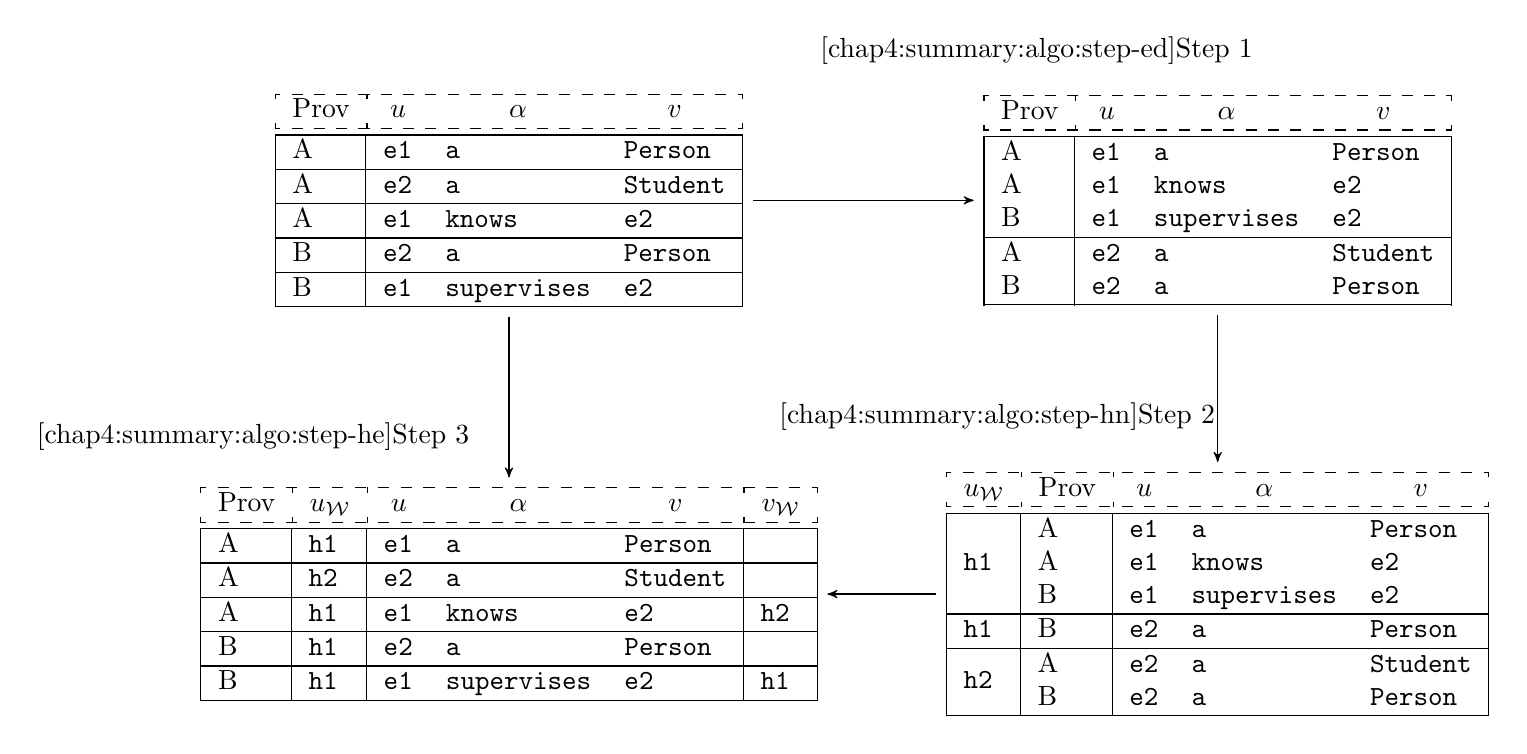
\begin{tikzpicture}[->,>=stealth',node distance=6.5cm]
\node (data) {
\begin{tabular}{|l|lll|}
\hdashline
\multicolumn{1}{:c}{Prov} & \multicolumn{1}{:c}{$u$} & \multicolumn{1}{c}{$\alpha$} & \multicolumn{1}{c:}{$v$} \\
\hdashline
\hline
A & \texttt{e1} & \texttt{a} & \texttt{Person} \\
\hline
A & \texttt{e2} & \texttt{a} & \texttt{Student} \\
\hline
A & \texttt{e1} & \texttt{knows} & \texttt{e2} \\
\hline
B & \texttt{e2} & \texttt{a} & \texttt{Person} \\
\hline
B & \texttt{e1} & \texttt{supervises} & \texttt{e2} \\
\hline
\end{tabular}
};

\node[right of = data,xshift=2.5cm] (edesc) {
\begin{tabular}{|l|lll|}
\hdashline
\multicolumn{1}{:c}{Prov} & \multicolumn{1}{:c}{$u$} & \multicolumn{1}{c}{$\alpha$} & \multicolumn{1}{c:}{$v$} \\
\hdashline
\hline
A & \texttt{e1} & \texttt{a} & \texttt{Person} \\
A & \texttt{e1} & \texttt{knows} & \texttt{e2} \\
B & \texttt{e1} & \texttt{supervises} & \texttt{e2} \\
\hline
A & \texttt{e2} & \texttt{a} & \texttt{Student} \\
B & \texttt{e2} & \texttt{a} & \texttt{Person} \\
\hline
\end{tabular}
};

\node[below of = edesc,yshift=1.5cm] (gsv) {
\begin{tabular}{|l|l|lll|}
\hdashline
\multicolumn{1}{:c}{$u_\mathcal{W}$} & \multicolumn{1}{:c}{Prov} & \multicolumn{1}{:c}{$u$} & \multicolumn{1}{c}{$\alpha$} & \multicolumn{1}{c:}{$v$} \\
\hdashline
\hline
\multirow{3}{*}{\texttt{h1}} & A & \texttt{e1} & \texttt{a} & \texttt{Person} \\
& A & \texttt{e1} & \texttt{knows} & \texttt{e2} \\
& B & \texttt{e1} & \texttt{supervises} & \texttt{e2} \\
\hline
\texttt{h1} & B & \texttt{e2} & \texttt{a} & \texttt{Person} \\
\hline
\multirow{2}{*}{\texttt{h2}} & A & \texttt{e2} & \texttt{a} & \texttt{Student} \\
& B & \texttt{e2} & \texttt{a} & \texttt{Person} \\
\hline
\end{tabular}
};

\node[below of = data,yshift=1.5cm] (join2) {
\begin{tabular}{|l|l|lll|l|}
\hdashline
\multicolumn{1}{:c}{Prov} & \multicolumn{1}{:c}{$u_\mathcal{W}$} & \multicolumn{1}{:c}{$u$} & \multicolumn{1}{c}{$\alpha$} & \multicolumn{1}{c:}{$v$} & \multicolumn{1}{:c:}{$v_\mathcal{W}$} \\
\hdashline
\hline
A & \texttt{h1} & \texttt{e1} & \texttt{a} & \texttt{Person} & \\
\hline
A & \texttt{h2} & \texttt{e2} & \texttt{a} & \texttt{Student} &  \\
\hline
A & \texttt{h1} & \texttt{e1} & \texttt{knows} & \texttt{e2} & \texttt{h2} \\
\hline
B & \texttt{h1} & \texttt{e2} & \texttt{a} & \texttt{Person} &  \\
\hline
B & \texttt{h1} & \texttt{e1} & \texttt{supervises} & \texttt{e2} & \texttt{h1} \\
\hline
\end{tabular}
};

\node at ($ (edesc) + (-2.3,1.9) $) {\hyperref[chap4:summary:algo:step-ed]{Step 1}};
\node at ($ (gsv) + (-2.8,2.25) $) {\hyperref[chap4:summary:algo:step-hn]{Step 2}};
\node at ($ (join2) + (-3.25,2) $) {\hyperref[chap4:summary:algo:step-he]{Step 3}};

\path
(data) edge (edesc)
(data) edge (join2)
(edesc) edge (gsv)
(gsv) edge (join2)
;
\end{tikzpicture}

		}
		\caption{The input data is a set of edges, one per row. The column $\mathcal{L}^D$ indicates the provenance of the edge. The columns $u_\mathcal{V}$ and $v_\mathcal{V}$ represents the sumnodes associated with the node $u$ and $v$, respectively. The ownership of \texttt{e1} is A, the dataset B owns \texttt{e2}. The Step~2 assigns the sumnodes according to the function \texttt{GetSumnode\textsubscript{i}} in Algorithm~\ref{alg:id-summary}.}
		\label{tab:id-algo-ex}
	\end{subfigure}
	\quad
	\begin{subfigure}{.8\textwidth}
		\centering
		\resizebox{.8\textwidth}{!}{
			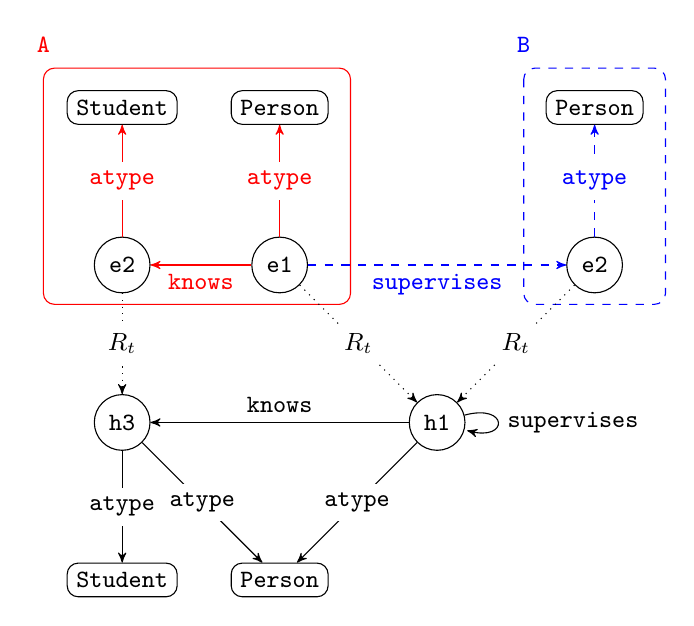
\begin{tikzpicture}[every node/.style={font=\ttfamily\small},main node/.style={draw,circle},type node/.style={rounded corners,draw},->,>=stealth',node distance=2cm]
\node[main node] (e1) {e1};
\node[main node,left of = e1] (e2) {e2};

\node[type node,above of = e1] (Aperson) {Person};
\node[type node,above of = e2] (Astudent) {Student};

\node[main node,right of = e1,xshift=2cm] (Be2) {e2};
\node[type node,above of = Be2] (Bperson) {Person};

\coordinate (Ax) at ($ (Astudent) + (-1,.5) $);
\coordinate (Ay) at ($ (e1) + (.9,-.5) $);
\draw[rounded corners,red]  (Ax) node[yshift=.3cm] {\textbf{A}} rectangle (Ay);

\coordinate (Bx) at ($ (Bperson) + (-.9,.5) $);
\coordinate (By) at ($ (Be2) + (.9,-.5) $);
\draw[rounded corners,dashed,blue]  (Bx) node[yshift=.3cm] {\textbf{B}} rectangle (By);

\node[main node,below of = e1,xshift=2cm] (h1) {h1};
\node[main node,below of = e2] (h3) {h3};

\node[type node,below of = h1,xshift=-2cm] (person) {Person};
\node[type node,below of = h3] (student) {Student};

\path
(e1) edge[red] node[fill=white] {\gls{atype}} (Aperson)
		edge[red] node[below] {knows} (e2)
(e2) edge[red] node[fill=white] {\gls{atype}} (Astudent)
(Be2) edge[blue,dashed] node[fill=white] {\gls{atype}} (Bperson)
(e1) edge[blue,dashed] node[below] {supervises} (Be2)

(e1) edge[dotted] node[fill=white] {$R_t$} (h1)
(e2) edge[dotted] node[fill=white] {$R_t$} (h3)
(Be2) edge[dotted] node[fill=white] {$R_t$} (h1)

(h1) edge[loop right] node[right] {supervises} (h1)
(h1) edge node[above] {knows} (h3)

(h3) edge node[fill=white] {\gls{atype}} (person)
		edge node[fill=white] {\gls{atype}} (student)
(h1) edge node[fill=white] {\gls{atype}} (person)
;
\end{tikzpicture}
		}
		\caption{Depiction of the \emph{Types} summary created in Figure~\ref{tab:id-algo-ex}. The edges which provenance is A are solid red, and those which provenance is B are dashed blue.}
		\label{fig:id-algo-ex}
	\end{subfigure}
	\caption{Example of the \emph{Types} summarisation $R_t$ in the case of inter-linked datasets.}
\end{figure}

\subsection{Implementations}

We present in this section two implementations of the graph summarisation, a first one based on SPARQL and then a second based on MapReduce~\cite{dean:2004:msd}. We present only the implementations of the Algorithm~\ref{alg:summary} for the summarisation of a single dataset. We outline below the required operators of the graph summarisation algorithm.
\begin{labeling}{\textbf{\underline{Step 1:}}}
\item[\textbf{\underline{Step 1:}}] In this step, we need a \emph{group} operator in order to build the entity description \gls{edesc}.
\item[\textbf{\underline{Step 2:}}] In this step we create the sumnode associated to a node according to its entity description. Therefore, we need a \emph{projection} operator in order to extract the features of the summarisation relation. We note that a feature can be multi-valued, which needs to be taken into account as well. The creation of the sumnode from the extracted features requires an \emph{object invention}~\cite{hull:1989:usi} operator.
\item[\textbf{\underline{Step 3:}}] The materialisation of the sumedges requires a \emph{join} operator through which we can retrieve the sumnode(s) associated with the source and target nodes.
\item[\textbf{\underline{Step 4:}}] As in Step~1 we need a group operator in order to aggregate sumnodes and sumedges, possibly computing \emph{statistics} at the same time.
\end{labeling}

\subsubsection{SPARQL implementation}

In this section, we describe an implementation of the graph summarisation algorithm based on SPARQL. The SPARQL query language is rich enough for us to only rely on it for the summary generation.
The Figure~\ref{fig:sparql-gs} shows the SPARQL query for generating a graph summary, and the query in Figure~\ref{fig:relation-sparql} is an example of a summarisation relation, i.e., \emph{Types} summarisation relation $R_t$.

\minisec{Operators}

SPARQL provides the operator \texttt{GROUP BY} which can be used to group data over a set of variables. The projection operator is implemented using a \texttt{SELECT} query. In the case of a multi-valued variable, we use the \texttt{GROUP\_CONCAT} operator which allows to concatenate all the values into a single literal. The object invention is performed thanks to built-in hash functions. In a SPARQL query, patterns which reuse some variables for either subject, predicate, or object components create implicitly a join. The computation of statistics can be performed using the built-in aggregate function in conjunction with the \texttt{GROUP BY} operator, e.g., \texttt{COUNT}. Thanks to the CONSTRUCT operator, we are able to create the graph summary directly from the query.

\minisec{Step 1 and Step 2}

In the Figure~\ref{fig:relation-sparql}, we extract the features relevant for the relation, e.g., the type values in this example. We note the use of the \texttt{ORDER BY} in the Figure~\ref{fig:relation-sparql} so to ensure that an unique ``identifier'' is created for the set of features thanks to the built-in hash function \texttt{SHA1}. We use the aggregate \texttt{GROUP\_CONCAT} in order to pass a single literal to SHA1, since an entity can be associated with multiple types.

\minisec{Step 3}

In the Figure~\ref{fig:sparql-gs}, the lines 4-7 (resp., lines 14-17) represent the summarisation relation, of which the Figure~\ref{fig:relation-sparql} is an example. The first block associates a sumnode to the variable on the subject position \emph{?s}, and the second block to the variable on the object position \emph{?o}, changing the name of projected variables appropriately for the object in the query of Figure~\ref{fig:relation-sparql}.

The sumedge materialisation is done on the line~11: the sumnode of the source node is retrieved thanks to the variable \emph{?s} that is projected by the sub-query in line~6; similarly for the target node thanks to the variable \emph{?o} returned by the sub-query line~16.
On lines 9 and 19, we create a URI for the source and target sumnodes, respectively.

On line 22, we consider the case when there is no sumnode associated with the object variable. This can happen if the object is a literal, or if no feature can be extracted for the resource. Since we are concerned with the graph structure with the graph summary, we need to keep the type value. Therefore, we add the condition on line 25 which corresponds to the line~4 in Algorithm~\ref{alg:summary}.
The empty string in the \emph{else} clause represents the sumnode $\varnothing$ in the graph summary.

\begin{remark}
This works only if the ontology is not inside the processed dataset, since the type value would be lost by the sumnode URI creation.
\end{remark}

\minisec{Step 4}

It is possible to assign some statistics about the summarisation when generating the sumnodes and sumedges. This requires again additional \texttt{GROUP BY} operations that are not depicted in the figure. However, we need then to reify the statistics in RDF since we use the \texttt{CONSTRUCT} operator in the query. This is further discussed in the Section~\ref{chap03:summary-rdf}.

\begin{remark}
If we use \texttt{CONSTRUCT} as the query form and we want to keep statistics about the summarisation, we need first to wrap the query into another one in which the aggregation is done. Then, we apply the \texttt{CONSTRUCT} query form on top. The reason is that that query form does not allow for aggregation operators such as \texttt{COUNT} in its clause.
\end{remark}

\begin{figure}
	\centering
	\begin{subfigure}{\textwidth}
		\centering
		{\footnotesize
			\begin{minted}[linenos,frame=lines,framesep=4mm]{sparql}
SELECT ?s (SHA1(GROUP_CONCAT(?t; separator = ",")) AS ?sID) {
    SELECT DISTINCT ?s ?t {
        ?s a ?t
    }
    ORDER BY ?t
}
GROUP BY ?s
			\end{minted}
		}
		\caption{Summarisation relation $R_t$}
		\label{fig:relation-sparql}
	\end{subfigure}
	\qquad
	\begin{subfigure}{\textwidth}
		\centering
		{\footnotesize
			\begin{minted}[linenos,frame=lines,framesep=4mm]{sparql}
CONSTRUCT {
    ?hs ?p ?ho
} WHERE {
    {
        # Sumnode features of the subject based on the summarisation relation
        ...
    }
    # Subject sumnode URI creation based on ?sID
    BIND(URI(CONCAT("http://example.org/", ?sID)) AS ?hs)

    ?s ?p ?o

    OPTIONAL {
        {
            # Sumnode features of the object based on the summarisation relation
            ...
        }
        # Object sumnode URI creation based on ?oID
        BIND(URI(CONCAT("http://example.org/", ?oID)) AS ?ho2)
    }
    # Support case when ?o has no features
    BIND(IF(
        BOUND(?oID),
        ?ho2,
        IF(?p = rdf:type, ?o, "")
    ) AS ?ho)
}
\end{minted}

		}
		\caption{SPARQL query that generates the graph summary in the \texttt{CONSTRUCT} clause}
		\label{fig:sparql-gs}
	\end{subfigure}
	\caption{SPARQL-based graph summarisation over a single dataset}
	\label{fig:gs-sparql-all}
\end{figure}

\subsubsection{MapReduce Implementation}

In this section, we describe an implementation of the graph summarisation algorithm based on MapReduce~\cite{dean:2004:msd}, which is a batch-processing framework that eases distributed operations over massive amount of data. The unit of work in MapReduce, called a \emph{job}, is composed of two operations: a \emph{mapper} and a \emph{reducer}. The mapper emits key-value pairs, and the reducer receives all the pairs associated to a same key.

\paragraph{Cascading.}

We developed the solution using Cascading\footnote{\url{http://www.cascading.org/projects/cascading/}}, which is a feature-rich API for defining and executing complex, scale-free, and fault-tolerant data processing workflows on a MapReduce cluster (e.g., Hadoop\footnote{http://hadoop.apache.org/}). The API lets the developer to quickly assemble complex processes without having to worry about the MapReduce paradigm. The Cascading model is based on the processing of ``tuples'', which can be seen as database records, thanks to operators that filter, join, aggregate, \ldots.  In the algorithms to follow, we represent a tuple using the set notation $\{\ldots\}$.

A Cascading flow is defined as a pipeline of such operators that connects data ``sources'' to ``sinks'' outputs. A flow can be composed of several ``pipes'', which represent a set of operations. The Cascading flow forms a directed acyclic graph, which is then converted into a sequence of MapReduce jobs that can be executed on the cluster.

The Figure~\ref{fig:summary-cascading} depicts the Cascading flow of the graph summarisation. A node represent an operation over the incoming tuples, which if superscripted with \emph{GB} involves an aggregate operation. The triangle-shaped nodes represent points in the flow where the data is written to or read from.

\minisec{Dictionaries}

Read and write (I/O) operations on disk are a major cause of performance degradation of MapReduce jobs. In order to avoid moving the data across the MapReduce cluster, we compute a set of \emph{dictionaries} that map a \emph{unique number} to a vocabulary term, i.e., either an attribute or a type. We then use this unique number throughout the graph summary computation, decreasing the amount of data copied across the cluster, but also improving operations such as joins.

The Figure~\ref{fig:dict-cascading} depicts the Cascading flow for creating the dictionaries. The edges $(u, \alpha, v) \in A$ of the graph $G$ are parsed, then a fork is done with regards to the attribute. We use the HFile~\cite{hfile} data structure as the dictionary backend. In our experiments, this marked a significant performance improvement compared to the Hadoop's MapFile~\cite{mapfile}. We use the DistributedCache\footnote{\url{https://hadoop.apache.org/docs/r1.2.1/api/org/apache/hadoop/filecache/DistributedCache.html}} in order to make the dictionaries accessible to all nodes of the MapReduce cluster.

The unique number a dictionary uses is computed using the MurmurHash3~\cite{murmurhash3-gcode,murmurhash3-blog} hash function. To further improve the performance of the summarisation, we hash the identifier of the nodes, i.e., the URI in the case of RDF data. A majority of the computation involves comparisons against these identifiers; thus using numbers instead of plain text improves shuffling operations in the MapReduce framework. In order to reduce potential hash collisions, we use the \emph{128bit} version of MurmurHash3.

Thanks to the dictionaries, the computation load over the two expensive join operations is decreased. Indeed, we only need to join data composed of unique numbers, without copying the plain text data across the MapReduce cluster which would increase the I/O. The entity description is needed only for the sumnode creation step. Once created, the computation can be abstracted from the actual data and use unique numbers instead. We use the dictionaries in the last step of the summarisation, which consist of the reification of the graph summary in RDF, intended for human consumption.

\minisec{Step 1}

The computation of a sumnode identifier requires all the information about an entity. Since the input data consist of an edge per tuple, we need to compute the entity description \gls{edesc} which is depicted by the Step~1 in the Figure~\ref{fig:va-cascading}. After parsing the input data, we aggregate the tuples based on the entity $u$. Cascading provides the \emph{GroupBy} operator to do so.
%In the case of summarising a collection of datasets, we include the dataset label as the group key, in order to handle correctly the statement authority.

Depending on the summarisation relation, more or less information about an entity is needed. In the relations presented in this thesis such as the \emph{IO Attributes} relation $R_{ioa}$, attributes of \emph{incoming} edges are required. We retrieve such information with no extra MapReduce job compared to others. The difference is in the amount of data aggregated.

The Algorithm~\ref{alg:inv-edge} describes the mapper function of the entity description creation to which we add the incoming edges. The mapper function takes the edge as input, and emits a tuple containing three elements. The underlined element represents the \emph{key} of the tuple. In the reducer function, we collect all the edges having the same hash key. If necessary, we can differentiate between incoming and outgoing edge thanks to the emitted flag.

\begin{algorithm}
	\DontPrintSemicolon
	\SetKwProg{Fn}{Function}{:}{end}
	\SetKwFunction{hash}{hash}
	\SetKwFunction{emit}{emit}
	\SetKwFunction{map}{map}
	\KwIn{a tuple containing an edge $(u, \alpha, v) \in A$.}
	\KwOut{a tuple containing\begin{inparaenum}[(1)]
			\item the hash value of the entity;
			\item a flag indicating whether the edge is incoming; and
			\item the edge.
		\end{inparaenum}}
	\BlankLine
	\tcp{Underlined tuple elements define the key within the MapReduce framework}
	\Fn{\map{$\left\lbrace\;(u, \alpha, v)\;\right\rbrace$}}{
		\emit{\{ \underline{\hash{$u$}}, 0, $(u, \alpha, v)$ \}}\;
		\tcp{``Reverse'' the edge direction}
		\emit{\{ \underline{\hash{$v$}}, 1, $(v, \alpha, u)$ \}}\;
	}
	\caption{Entity description expanded with incoming edges}
	\label{alg:inv-edge}
\end{algorithm}

\minisec{Step 2}

In order to generate unique identifiers for sumnodes, we extract features relevant to the summarisation relation from the entity description. For instance, we need the type values for the relation $R_t$, and for $R_a$ we are interested in the attributes. The projection operator as well as the handling of multi-valued feature are then performed programmatically, using a \emph{mapper}.

The Algorithm~\ref{alg:mapper-rt} describes the implementation of the $R_t$ relation, which stands as an example of Step~2 in the figure. We retrieve the type values associated with the node $u$ on lines~2-5. The object invention is performed on line~6, where we emit the input tuple to which we add the identifier of the sumnode, i.e., the hash of the set of types.

\begin{algorithm}
	\DontPrintSemicolon
	\SetKwProg{Fn}{Function}{:}{end}
	\SetKwFunction{hash}{hash}
	\SetKwFunction{emit}{emit}
	\SetKwFunction{map}{map}
	\SetKwData{types}{types}
	\KwIn{a tuple containing the hash value of a node $u$, and the entity description $\gls{edesc}(u)$ of that node.}
	\KwOut{a tuple containing\begin{inparaenum}[(1)]
			\item the sumnode identifier;
			\item the hash value of $u$; and
			\item the entity description $\gls{edesc}(u)$ of that node.
		\end{inparaenum}}
	\BlankLine
	\Fn{\map{$\{ \hash{u}, \gls{edesc}(u) \}$}}{
		\types $\gets$ [ ]\;
		\ForEach{$(u, \alpha_i, v_i) \in \gls{edesc}(u)$}{
			\If(\tcp*[h]{$\alpha_i$ is a type attribute}){$\alpha_i == \gls{atype}$}{
				$\types[i] \gets v_i$\;
			}
		}
		\emit{$\{ \hash{\types}, \hash{u}, \gls{edesc}(u) \}$}\;
	}
	\caption{\emph{Types} summarisation relation $R_t$}
	\label{alg:mapper-rt}
\end{algorithm}

\minisec{Step 3}
\label{chap03:algo:edge-materialisation}

We materialise the sumedges in two distinct processes, depicted by the Step~3a and Step~3b in the figure. The reason is to decrease the amount of data joined with the sumnode mappings from Step~2. To do so, we filter out in Step~3b the edges which target node is a sink --- in RDF, this means to remove the edges which object is a \emph{literal}. Also, we filter edges which have the type attribute. The reason is that the target node, which here is the type value, does not represent an entity. This is represented by the line~4 of the Algorithm~\ref{alg:summary}.

In Step~3a, we create the sumedges which \emph{target} sumnode is $\varnothing$. In Step~3b instead, we consider the sumedges which target might be defined --- it may not be if the target node is not mapped to any sumnode (Step~2 in the figure). We remark that the Step~3a requires no join. Indeed, we keep the entity description along with the sumnode identifier as a result of the Step~2 processing.

\minisec{Step 4}

We end both Step~3a and Step~3b with a grouping operation. In Step~3a, we group all the tuples sharing the same sumnode identifier into a single tuple, computing some statistics if necessary, e.g., number of occurrences of an attribute, or the number of \emph{nodes} mapped to the sumnode. In Step~3b, we group the tuples sharing both the source and target sumnodes as well as the attribute, thus forming the sumedges. Similarly, we may compute statistics about the sumedge in this step, e.g., the number of occurrences of a labelled edges connecting any nodes that were mapped to the adjacent sumnodes.

\begin{figure}
	\centering
	\begin{subfigure}{\textwidth}
		\centering
		\resizebox{.6\textwidth}{!}{
			\usetikzlibrary{shapes,arrows}

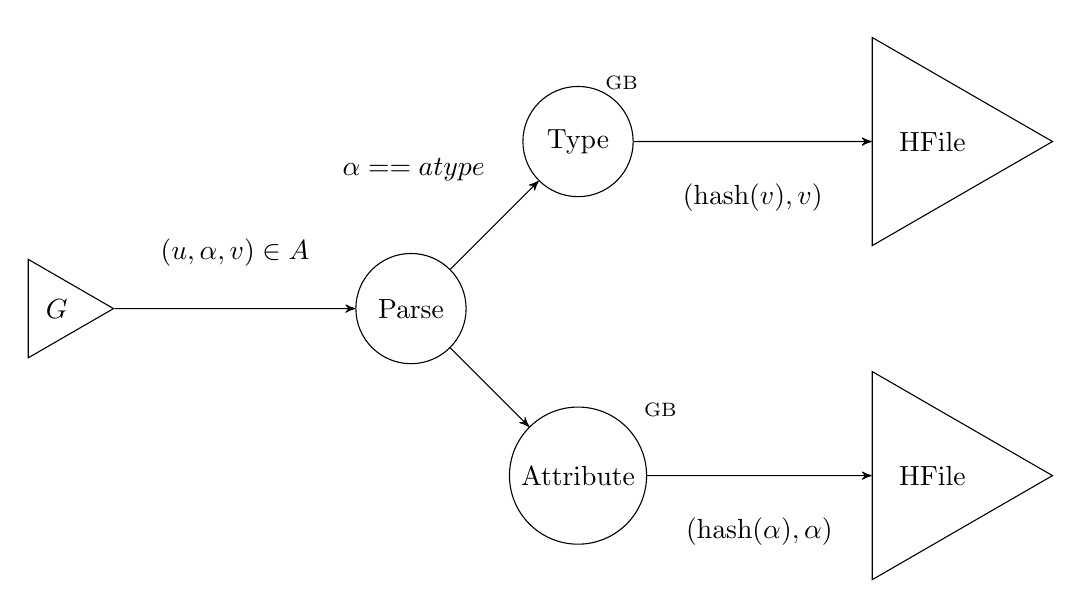
\begin{tikzpicture}[->,>=stealth',node distance=3cm,minimum height=1.4cm]

\node[draw,regular polygon, regular polygon sides=3,shape border rotate=-90] (in) {$G$};

\node[draw,circle,right of = in,xshift=1.5cm] (parse) {Parse};

\node[draw,circle,above right of = parse] (type) {Type};
\node [above right of = parse,label={[label distance=.1cm]10:\scriptsize{GB}}] {};

\node[draw,circle,below right of = parse] (attribute) {Attribute};
\node [below right of = parse,label={[label distance=.6cm]10:\scriptsize{GB}}] {};

\node[right of = type,draw,regular polygon, regular polygon sides=3,shape border rotate=-90,xshift=1.5cm] (tout) {HFile};
\node[right of = attribute,draw,regular polygon, regular polygon sides=3,shape border rotate=-90,xshift=1.5cm] (aout) {HFile};

\path
(in) edge node[above] {$(u, \alpha, v) \in A$} (parse)
(parse) edge node[above left] {$\alpha == \gls{atype}$} (type)
(parse) edge (attribute)
(type) edge node[below] {$(\text{hash}(v), v)$} (tout)
(attribute) edge node[below] {$\left(\text{hash}(\alpha), \alpha\right)$} (aout)
;
\end{tikzpicture}
		}
		\caption{Dictionary computation}
		\label{fig:dict-cascading}
	\end{subfigure}
	\qquad
	\begin{subfigure}{\textwidth}
		\centering
		\resizebox{\textwidth}{!}{
			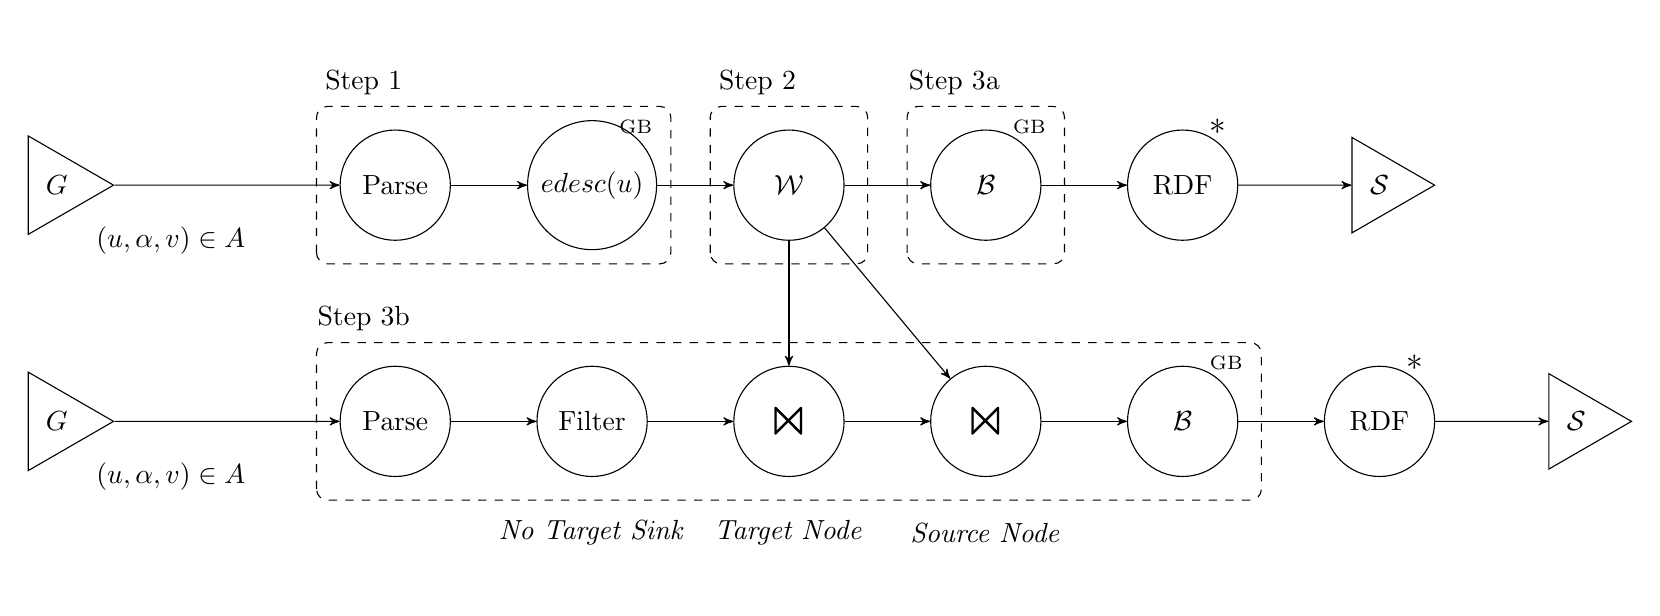
\begin{tikzpicture}[->,>=stealth',node distance=2.5cm,minimum height=1.4cm]

\node[draw,regular polygon, regular polygon sides=3,shape border rotate=-90] (in) {$G$};

\node[draw,circle,right of = in,xshift=1.8cm] (parse) {Parse};
\node[draw,circle,right of = parse] (edesc) {$\glssymbol{edesc}(u)$};
\node [right of = parse,label={[label distance=.1cm]10:\scriptsize{GB}}] {};

\node[below of = in,draw,regular polygon, regular polygon sides=3,shape border rotate=-90,yshift=-.5cm] (in2) {$G$};
\node[draw,circle,right of = in2,xshift=1.8cm] (parse2) {Parse};

\node [draw,circle,label={-90:\emph{No Target Sink}},right of = parse2] (filter) {Filter};

\node[draw,circle,right of = edesc] (gsv) {$\mathcal{W}$};

\node[draw,circle,below of = gsv,label={-90:\emph{Target Node}},yshift=-.5cm] (joinsub) {{\huge $\Join$}};
\node[draw,circle,right of = joinsub,label={-90:\emph{Source Node}}] (joinobj) {{\huge $\Join$}};

\node[draw,circle,right of = joinobj] (relagg) {$\mathcal{B}$};
\node [right of = joinobj,label={[label distance=.1cm]10:\scriptsize{GB}}] {};

\node[draw,circle,right of = gsv] (attagg) {$\mathcal{B}$};
\node [right of = gsv,label={[label distance=.1cm]10:\scriptsize{GB}}] {};

\node[draw,circle,right of = attagg] (attrdf) {RDF};
\node [right of = attagg,label={[label distance=.1cm]10:\scriptsize{{\large $*$}}}] {};
\node[draw,circle,right of = relagg] (relrdf) {RDF};
\node [right of = relagg,label={[label distance=.1cm]10:\scriptsize{{\large $*$}}}] {};

\node[right of = attrdf,draw,regular polygon, regular polygon sides=3,shape border rotate=-90] (attout) {$\mathcal{S}$};
\node[right of = relrdf,draw,regular polygon, regular polygon sides=3,shape border rotate=-90] (relout) {$\mathcal{S}$};


\coordinate (p1x) at ($ (parse) + (-1,-1) $);
\coordinate (p1y) at ($ (edesc) + (1,1) $);
\draw[rounded corners,dashed]  (p1x) node[yshift=2.3cm,xshift=.6cm] {Step 1} rectangle (p1y);
\coordinate (p2x) at ($ (gsv) + (-1,-1) $);
\coordinate (p2y) at ($ (gsv) + (1,1) $);
\draw[rounded corners,dashed]  (p2x) node[yshift=2.3cm,xshift=.6cm] {Step 2} rectangle (p2y);
\coordinate (p3x) at ($ (attagg) + (-1,-1) $);
\coordinate (p3y) at ($ (attagg) + (1,1) $);
\draw[rounded corners,dashed]  (p3x) node[yshift=2.3cm,xshift=.6cm] {Step 3a} rectangle (p3y);
\coordinate (p4x) at ($ (parse2) + (-1,-1) $);
\coordinate (p4y) at ($ (relagg) + (1,1) $);
\draw[rounded corners,dashed]  (p4x) node[yshift=2.3cm,xshift=.6cm] {Step 3b} rectangle (p4y);


\path
(in) edge node[below,near start] {$(u, \alpha, v) \in A$} (parse)
(in2) edge node[below,near start] {$(u, \alpha, v) \in A$} (parse2)
(parse) edge (edesc)
(edesc) edge (gsv)
(gsv) edge (joinsub)
(parse2) edge (filter)
(filter) edge (joinsub)
(gsv) edge (joinobj)
(joinsub) edge (joinobj)
(joinobj) edge (relagg)
(gsv) edge (attagg)
(relagg) edge (relrdf)
(attagg) edge (attrdf)
(relrdf) edge (relout)
(attrdf) edge (attout)
;
\end{tikzpicture}

		}
		\caption{Sumedge and sumnode creation}
		\label{fig:va-cascading}
	\end{subfigure}
	\caption{Graph summarisation using the Cascading framework. A node represent an operation over the incoming tuples, which if superscripted with GB involves an aggregate operation, i.e., there is a \texttt{GROUP BY} operation. The $*$ superscript over the RDF nodes indicates that the dictionary is used for mapping the data back into plain text. The triangle-shaped nodes represent points in the flow where the data is written to or read from.}
	\label{fig:summary-cascading}
\end{figure}

\subsubsection{Discussion}

Apart from the use of machine expensive operators such as \texttt{ORDER BY} or \texttt{GROUP\_CONCAT}, we remark that the SPARQL query of the summarisation relation is duplicated two times. Therefore, this is an inefficient part of the query depicted in Figure~\ref{fig:sparql-gs}. Depending on the query planner of the SPARQL engine, this duplication might be spotted so to avoid computing twice the same pattern.

In comparison, the MapReduce-based one allows the summarisation to scale to much larger graphs. Indeed, in our experiments the SPARQL-based implementation is able to summarise graphs up to 20M edges only. A major obstacle to scale to larger graphs are the constraints imposed by SPARQL endpoints, e.g., limiting the number of rows returned by a \texttt{SELECT} query form, or query execution time-outs. Instead, the MapReduce implementation is able to scale to billions of edges, e.g., 2B with Freebase\footnote{\url{https://www.freebase.com/}} or even 30B with the Sindice dataset.

%\begin{figure}
%	\pgfplotstableread{
%		x         y    y-max  y-min
%		10        0.209219 0.34681420 0.17105213
%		50 3.823154 4.95525438 3.56146301
%		100 1.790687 3.17752483 1.64086531
%		500 8.759389 16.14254738 8.10480235
%	}{\mytable}
%	\begin{tikzpicture}
%	\begin{axis} [
%	ymin=0,
%	symbolic x coords={10,50,100,500},
%	xtick=data
%	]
%	\addplot [ybar, fill=gray!50] 
%	plot [error bars/.cd, y dir=both, y explicit]
%	table [y error plus=y-max, y error minus=y-min] {\mytable};
%	\end{axis} 
%	\end{tikzpicture}
%\end{figure}

\subsection{Graph Summary Lattice}

There exists several possible summarisation relations, each resulting in a graph summary that exhibits different properties. In the Section~\ref{chap03:sec:quality}, we discuss the impact of the relation on the \emph{precision} of a graph summary with regards to the original graph. There is no graph summary that fits all use cases, a summary suitable for one might not be for another. In this section, we describe how various summarisation relations can be ordered into a \emph{lattice}. Thus, we can reuse previous computations where a graph summary can result from another one, instead from the original graph.

A \emph{lattice} is a \emph{partially ordered} set that contains an \emph{infimum} and a \emph{supremum}. The infimum is an element of the set that is ``smaller'', according to the partial order, than all other elements. Conversely, a supremum is an element that is larger than any other element.

For the set of summarisation relations $\mathcal{R}$, we denote with $\sqsubseteq$ the partial order on $\mathcal{R}$. We order the relations based on their definition: two summarisation relations can be ordered if one can be expressed with the other. In this set, the infimum is the identity relation that maps the graph to itself, and the supremum is the relation that maps all nodes to a single sumnode.

\begin{definition}[Partial Order $\sqsubseteq$]
Let $G=\left\langle V, A, l_V \right\rangle$ be a graph, $\mathcal{S}_1 = \left\langle \mathcal{V}_1, \mathcal{A}_1, l_{\mathcal{V}_1} \right\rangle$ be the summary of $G$ according to $R_1 \subseteq V \times \mathcal{V}_1$, and $\mathcal{S}_2 = \left\langle \mathcal{V}_2, \mathcal{A}_2, l_{\mathcal{V}_2} \right\rangle$ be the summary of $G$ according to $R_2 \subseteq V \times \mathcal{V}_2$.

We say that $R_1$ precedes $R_2$, noted as $R_1 \sqsubseteq R_2$, if there exists a relation $S \subseteq \mathcal{V}_1 \times \mathcal{V}_2$ such that $R_2$ is a \emph{composition} of $R_1$ and $S$:
$$
R_2 = S \circ R_1 = \left\lbrace (x, z) \in R_2 \mid \exists y \in \mathcal{V}_1 : (x, y) \in R_1 \wedge (y, z) \in S \right\rbrace 
$$
\end{definition}

\begin{proof}
We demonstrate here that the binary relation $\sqsubseteq$ is a partial order, i.e., that it is reflexive, antisymmetric, and transitive.
Let $G=\left\langle V, A, l_V \right\rangle$ be a graph, and for some set $A$, let $I_A = \left\lbrace (x, x) : x \in A \right\rbrace$ be the identity relation on $A$.
\begin{description}
\item[reflexivity:] Let $\mathcal{S} = \left\langle \mathcal{V}, \mathcal{A}, l_{\mathcal{V}} \right\rangle$ be the summary of $G$ according to $R \subseteq V \times \mathcal{V}$. We have $R = I_\mathcal{V} \circ R$, therefore $R \sqsubseteq R$.
\item[antisymmetry:] For $i \in \{1, 2\}$, let $\mathcal{S}_i = \left\langle \mathcal{V}_i, \mathcal{A}_i, l_{\mathcal{V}_i} \right\rangle$ be the summary of $G$ according to $R_i \subseteq V \times \mathcal{V}_i$. If we suppose $R_1 \sqsubseteq R_2 \wedge R_2 \sqsubseteq R_1$, then $\exists S \subseteq \mathcal{V}_1 \times \mathcal{V}_2$ and $\exists T \subseteq \mathcal{V}_2 \times \mathcal{V}_1$ such that $R_2 = S \circ R_1$ and $R_1 = T \circ R_2$. By substitution, we have $R_2 = S \circ T \circ R_2$. Hence, $S \circ T = I_{\mathcal{V}_2}$. Since the identity relation is a bijection, we have a \emph{one-to-one} mapping between $\mathcal{V}_1$ and $\mathcal{V}_2$. Therefore, we have $R_1 = R_2$.
\item[transitivity:] For $i \in \{1, 2, 3\}$, let $\mathcal{S}_i = \left\langle \mathcal{V}_i, \mathcal{A}_i, l_{\mathcal{V}_i} \right\rangle$ be the summary of $G$ according to $R_i \subseteq V \times \mathcal{V}_i$. If we suppose $R_1 \sqsubseteq R_2 \sqsubseteq R_3$, then $\exists S \subseteq \mathcal{V}_1 \times \mathcal{V}_2$ and $\exists T \subseteq \mathcal{V}_2 \times \mathcal{V}_3$ such that $R_2 = S \circ R_1$ and $R_3 = T \circ R_2$. Let $U \subseteq \mathcal{V}_1 \times \mathcal{V}_3$ be a relation defined as the composition of $S$ and $T$, i.e., $U = T \circ S$. Since the composition operation $\circ$ is associative, we have then $R_3 = U \circ R_1$. Therefore, $R_1 \sqsubseteq R_3$.
\end{description}
\end{proof}

The set of summarisation relations $\mathcal{R}$ can then be ordered according to $\sqsubseteq$. The Figure~\ref{fig:lattice} depicts the lattice that is formed by the partial order $\sqsubseteq$ for the relations presented in Section~\ref{sec:approximate}. We can then see that all summaries can be generated from the summary on $R_{ioat}$. In cases where the summary has significantly less edges and nodes than the original graph, this represents an increase of the summarisation performance.

\begin{figure}
	\centering
	\input{04-summary/figures/lattice}
	\caption{Lattice of the summarisation relations set according to the partial order $\sqsubseteq$}
	\label{fig:lattice}
\end{figure}

\paragraph{Example.}

The Figure~\ref{fig:rel-order} depicts the sumnodes built from two summarisation relations $R_t$ (dotted lines) and $R_{at}$ (dashed lines) over the graph on Figure~\ref{fig:graph}. The solid lines represent a relation $S \subseteq \mathcal{V}_{at} \times \mathcal{V}_t$, with which we have the order $R_{at} \sqsubseteq R_t$ between the two relations. With the $R_{at}$ relation, the nodes $N_6$ and $N_7$ belong to different sumnodes, while they belong to the same with the $R_t$ relation. The same $R_t$ summary is built from the original graph and from the $R_{at}$ summary. The partial order allows then to leverage pre-computed summaries in order to generate a new one.

\begin{figure}
	\centering
	\usetikzlibrary{arrows}

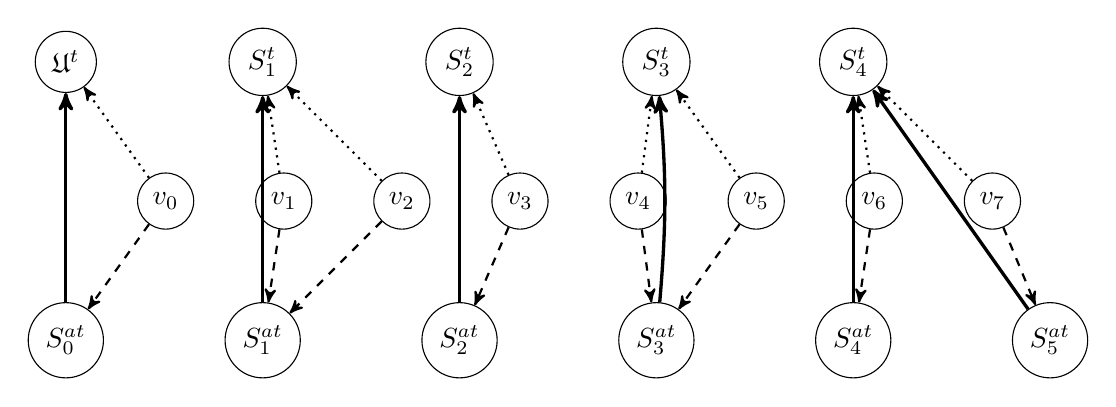
\begin{tikzpicture}[->,>=stealth',node distance=1.5cm,tnode/.style={node distance=2.5cm,draw,circle}]

\node[draw,circle] (0) {$v_0$};
\node[draw,circle,right of = 0] (1) {$v_1$};
\node[draw,circle,right of = 1] (2) {$v_2$};
\node[draw,circle,right of = 2] (3) {$v_3$};
\node[draw,circle,right of = 3] (4) {$v_4$};
\node[draw,circle,right of = 4] (5) {$v_5$};
\node[draw,circle,right of = 5] (6) {$v_6$};
\node[draw,circle,right of = 6] (7) {$v_7$};

\node[tnode,below left of = 0,xshift=.5cm] (ath0) {$S^{at}_0$};
\node[tnode,right of = ath0] (ath1) {$S^{at}_1$};
\node[tnode,right of = ath1] (ath2) {$S^{at}_2$};
\node[tnode,right of = ath2] (ath3) {$S^{at}_3$};
\node[tnode,right of = ath3] (ath4) {$S^{at}_4$};
\node[tnode,right of = ath4] (ath5) {$S^{at}_5$};

\node[tnode,above left of = 0,xshift=.5cm] (th0) {$\mathfrak{U}^t$};
\node[tnode,draw,circle,right of = th0] (th1) {$S^{t}_1$};
\node[tnode,draw,circle,right of = th1] (th2) {$S^{t}_2$};
\node[tnode,draw,circle,right of = th2] (th3) {$S^{t}_3$};
\node[tnode,draw,circle,right of = th3] (th4) {$S^{t}_4$};

\path
(0) edge[thick,dashed] (ath0)
(1) edge[thick,dashed] (ath1)
(2) edge[thick,dashed] (ath1)
(3) edge[thick,dashed] (ath2)
(4) edge[thick,dashed] (ath3)
(5) edge[thick,dashed] (ath3)
(6) edge[thick,dashed] (ath4)
(7) edge[thick,dashed] (ath5)

(0) edge[thick,dotted] (th0)
(1) edge[thick,dotted] (th1)
(2) edge[thick,dotted] (th1)
(3) edge[thick,dotted] (th2)
(4) edge[thick,dotted] (th3)
(5) edge[thick,dotted] (th3)
(6) edge[thick,dotted] (th4)
(7) edge[thick,dotted] (th4)

(ath0) edge[very thick] (th0)
(ath1) edge[very thick] (th1)
(ath2) edge[very thick] (th2)
(ath3) edge[very thick,bend right=5] (th3)
(ath4) edge[very thick] (th4)
(ath5) edge[very thick] (th4)
;
\end{tikzpicture}
	\caption{Sumnodes of summarisation relations $R_t$ and $R_{at}$ for the graph in Figure~\ref{fig:graph}. The dashed lines represent the $R_{at}$ relation, the dotted lines the $R_t$ relation, and the solid lines the relation derived from the partial order $\sqsubseteq$, i.e., $R_{at} \sqsubseteq R_t$. The nodes with superscript $t$ belong to the summary built from $R_t$, while the nodes with superscript $at$ belong to the summary built from $R_{at}$.}
	\label{fig:rel-order}
\end{figure}


%\input{04-summary/updates}

\section{Graph Summary Precision}
\label{chap03:sec:quality}

The quality of a summary depends on the summarisation relation used, which we discuss in this section in terms of volume of the graph and of precision of the summarized data.

\subsection{Summary Volume}

A summary is smaller if its size $\vert \mathcal{B} \vert$ and its order $\vert \mathcal{W} \vert$ are inferior to the size $\vert A \vert$ and the order $\vert V \vert$ of the data graph.

Apart from $R_{st}$, the presented summarisation relations in Section~\ref{sec:approximate} create a summary which is always smaller or equal to the data graph, since there is a one-to-one mapping from the data graph to the summary.

The $R_{st}$ relation may assign several equivalence classes to a node $u \in V$, i.e., when $\vert types(u) \vert > 1$. The order of a summary built from $R_{st}$ is at most equal to $\vert V_{st} \vert = \vert \mathcal{L}^T \vert$. However, in the worst case, its size can equal $\vert A_{st} \vert = \vert \mathcal{L}^T \vert ^d$, with $d$ being the diameter\footnote{The diameter $d$ of a graph $G$ is the maximum distance between any two nodes of the graph. The distance between two nodes is the number of edges in the shortest path that connects the two.} of the data graph. Indeed, every node of the data graph can be associated with all the types, i.e., $\forall u \in V, types(u) = \mathcal{L}^C$. Therefore when applying the relation $R_{st}$ over such a graph, we need for each path in $G$ to create an edge to each type for every node of the path.

The summary is sensitive to heterogeneous data graph. Indeed, there can be a node in a $\mathcal{S}_a$ summary for each element of the attribute powerset minus the empty set, i.e., $\vert V^{\sim_a} \vert = 2^{\vert \mathcal{L}^A \vert} - 1$. Such an order of the summary can be expected for any relation based on the set of attributes, i.e., the relations $R_{at}$, $R_{ioa}$, $R_{ioat}$, and $R_{fbt}$.

We note that reducing the volume of a summary comes with a price, that of reduced precision of the summary, which we discuss in the next section.

\subsection{Summary Error}

The confidence one may put on knowledge deduced from a summary has a more or less severe impact depending on the application. Also, the severity of an error depends on what information about the data graph is affected by the error. In this section, we introduce a model for measuring the precision of a summary.

\subsubsection{Error Model}

The graph summary is a summary of the \emph{structure} of the data graph. Therefore, errors in the summary boil down to the presence of invalid edges. A path, or a combination of paths, may exists in the summary $\mathcal{S}$, but not in the data graph $G$. This precision model accounts for the paths that exist in the summary but not in the data graph.

%The definition of the precision model requires the introduction of an order relation on the summary. A set of summaries over a same data graph can be ordered using the relation $\sqsubseteq$ \cite{Fernandez:1990:IEA:87626.87629}.
%For instance, if we consider the $\sim_{fbt}$ and $\sim_t$ summaries in Figures~\ref{fig:fbb-summary} and \ref{fig:classes-summary}, the nodes of $G$ in the equivalence classes $[N_1]^{\sim_{fbt}}$ and $[N_2]^{\sim_{fbt}}$ also belong to the equivalence class $[N_1]^{\sim_t}$. The equivalence classes of $\sim_{fbt}$ are then included in the equivalence classes of $\sim_t$. Therefore, the $\sim_{fbt}$-summary is inferior to the $\sim_t$-summary, noted as $\sim_{fbt} \sqsubseteq \sim_t$.
%
%\begin{definition}[$\sqsubseteq$ Ordering]
%Let $\sim_1$ and $\sim_2$ be two equivalences on a data graph $G$. There is a partial order $\sqsubseteq$ on the $\sim_1$ and $\sim_2$ summaries, noted $\sim_1 \sqsubseteq \sim_2$, if and only if: $\forall [x]^{\sim_1} \in V^{\sim_1}, \exists [x]^{\sim_2} \in V^{\sim_2}, [x]^{\sim_1} \subseteq [x]^{\sim_2}$.
%\end{definition}

As per the recursive definition of the $R_{fbt}$ relation based on bisimulation, a node in the $\mathcal{S}_{fbt}$ summary refers to nodes of $G$ that share the same \emph{incoming} and \emph{outgoing} paths. Thus, the $\mathcal{S}_{fbt}$ summary is the most precise summary for a data graph with regards to the structure, i.e., all paths in the summary do exist in the original data graph.

According to the partial ordering relation $\sqsubseteq$, a $\mathcal{S}_{fbt}$ summary is ``smaller'' than any of the other presented summaries, i.e., for any summarisation relation $R$ we have $R_{fbt} \sqsubseteq R$. Therefore, any edge on a summary can be inferred from the $\mathcal{S}_{fbt}$ summary. However, the converse is not necessarily true.
% Relations between two $\sim$-equivalence classes can be inferred between the included $\sim_{fbt}$-equivalence classes.

We define the set $Err(R)$ as the set of inferred edges that are erroneous, i.e., the edges that do exist in a summary, but not in the original graph. Since the summary $\mathcal{S}_{fbt}$ is the most precise with regards to the structure of the original graph, we use the summary $\mathcal{S}_{fbt}$ instead of the original graph $G$ to define the set $Err(R)$.

\begin{definition}[Summary Error $Err(R)$]
Let $G=\left\langle V, A, l_V \right\rangle$ be a graph, $\mathcal{S} = \left\langle \mathcal{W}, \mathcal{B}, l_{\mathcal{W}} \right\rangle$ be the summary of $G$ according to $R \subseteq V \times \mathcal{W}$, and $\mathcal{S}_{fbt} = \left\langle \mathcal{W}_{fbt}, \mathcal{B}_{fbt}, l_{\mathcal{W}_{fbt}} \right\rangle$ the bisimulation summary generated with the relation $R_{fbt}$.
The set $Err(R)$ is the set of edges between nodes of $\mathcal{S}_{fbt}$ that are inferred from $\mathcal{S}$ as per the $\sqsubseteq$ relation.
\begin{equation*}
\begin{split}
Err(R) = \{ & (u, \alpha, v) \in \mathcal{W}_{fbt} \times \mathcal{L}^A \times \mathcal{W}_{fbt} \mid \exists (x, y) \in V^2 :\\
 & (R(x), \alpha, R(y)) \in \mathcal{B} \wedge (R_{fbt}(x), \alpha, R_{fbt}(y)) \not \in \mathcal{B}_{fbt} \}
\end{split}
\end{equation*}
\end{definition}

We note that $Err(R)$ is equal to all possible combinations of nodes pair on $G$, keeping only the ones that exists in the summary $\mathcal{S}$ but not in the bisimulation summary $\mathcal{S}_{fbt}$.

\paragraph{Inferred Graph $\mathfrak{G}(R)$.}

We introduce the graph $\mathfrak{G}(R)$ as the graph $\mathcal{S}_{fbt}$ that is \emph{augmented} with inferred edges from the $Err(R)$ set. This graph is used for computing the set of true and false positive edges in Section~\ref{sec:edge-precision}.

\begin{definition}[Inferred Graph]
Let $G=\left\langle V, A, l_V \right\rangle$ be a graph, $\mathcal{S} = \left\langle \mathcal{W}, \mathcal{B}, l_{\mathcal{W}} \right\rangle$ be the summary of $G$ according to $R \subseteq V \times \mathcal{W}$, and $\mathcal{S}_{fbt} = \left\langle \mathcal{W}_{fbt}, \mathcal{B}_{fbt}, l_{\mathcal{W}_{fbt}} \right\rangle$ be the bisimulation summary of $G$ according to $R_{fbt}$ such that $R_{fbt} \sqsubseteq R$.

We call the \emph{inferred graph} $\mathfrak{G}(R) = \left\langle \mathcal{W}_{fbt}, \mathfrak{A}, l_{\mathcal{W}_{fbt}} \right\rangle$ the graph which nodes and edges are those of the bisimulation summary $\mathcal{S}_{fbt}$, augmented with the edges in $Err(R)$, i.e., $\mathfrak{A} = \mathcal{B}_{fbt} \cup Err(R)$.
\end{definition}

The Figure~\ref{fig:accuracy} depicts the inferred graph $\mathfrak{G}(R_t)$ according to the \emph{Types} summary $\mathcal{S}_t$ in Figure~\ref{fig:classes-summary}.
Sink nodes are omitted for clarity. The bisimulation summary $\mathcal{S}_{fbt}$ is depicted with solid lines, and the \emph{Types} summary $\mathcal{S}_t$ with dashed lines. Edges from the $Err(R_t)$ set are represented with grey dotted arrows.

Given that $R_{fbt} \sqsubseteq R_t$, the nodes $H^b_1$ and $H^b_2$ are mapped to the node $H^t_1$. Similarly, the nodes $H^b_4$ and $H^b_5$ are mapped to the node $H^t_3$. Since the edge $(H^t_1, works, H^t_3) \in \mathcal{B}_t$ exists, the edges labelled $works$ can then be inferred from the nodes $H^b_1$ and $H^b_2$ to $H^b_5$. Edges from the $Err(R_t)$ set cause the nodes $H^b_1$, $H^b_5$, and $H^b_6$ to be connected. This generates the path $works.location.capital$ that exists in the \emph{Types} summary, but not in the bisimulation summary, and by extension, in the original graph $G$.

\begin{figure}
	\centering
	\resizebox{\textwidth}{!}{
		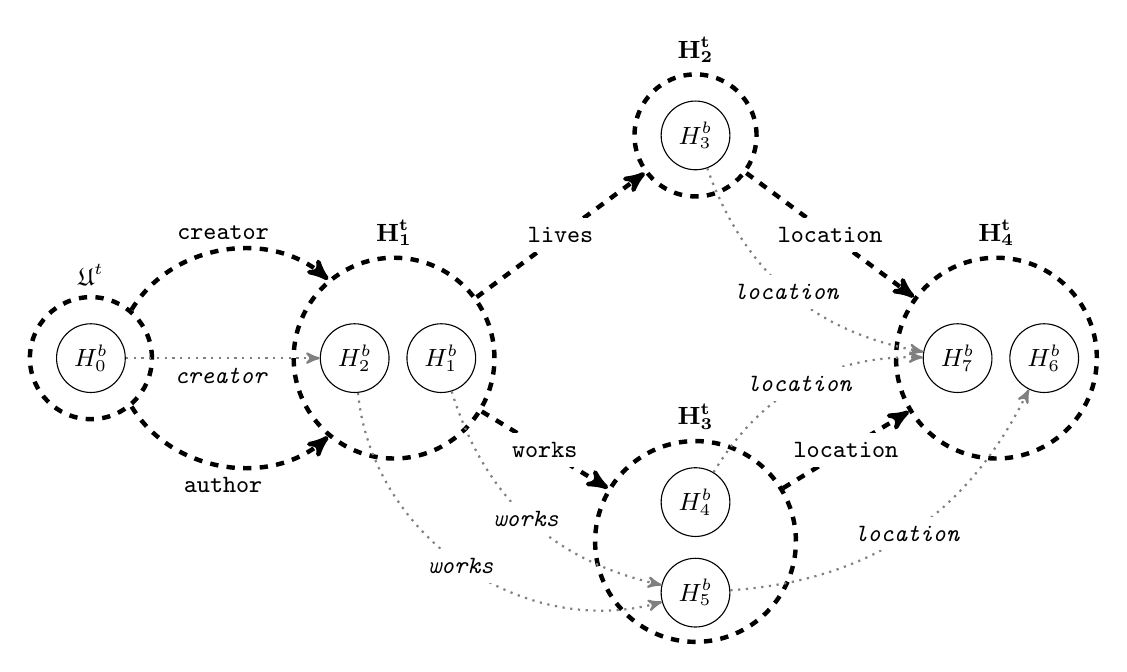
\begin{tikzpicture}[->,>=stealth',node distance=4cm,every node/.style={font=\small\ttfamily}]
%Bisim
\node[draw,circle] (b0) {$H^b_0$};

\node[draw,circle,right of = b0,xshift=-.65cm] (b1) {$H^b_2$};
\node[draw,circle,right of = b0,xshift=.45cm] (b2) {$H^b_1$};

\node[draw,circle,above right of = b2,xshift=.4cm,yshift=0cm] (b3) {$H^b_3$};

\node[draw,circle,below right of = b1,xshift=1.5cm,yshift=1cm] (b4) {$H^b_4$};
\node[draw,circle,below of = b4,yshift=2.85cm] (b5) {$H^b_5$};

\node[draw,circle,below right of = b3,xshift=.5cm,yshift=0cm] (b7) {$H^b_7$};
\node[draw,circle,above right of = b4,xshift=1.6cm,yshift=-1cm] (b6) {$H^b_6$};

%Types
\node[draw,circle,dashed,ultra thick,minimum size=1.55cm,label={90:$\mathfrak{U}^t$}] (t0) {};
\node[draw,circle,dashed,ultra thick,minimum size=2.55cm,label={90:$\mathbf{H^t_1}$},right of = t0,xshift=-.15cm] (t1){};
\node[draw,circle,dashed,ultra thick,minimum size=1.55cm,label={90:$\mathbf{H^t_2}$},above right of = t1,xshift=1cm,yshift=0cm] (t2){};
\node[draw,circle,dashed,ultra thick,minimum size=2.55cm,label={90:$\mathbf{H^t_3}$},below right of = t1,yshift=.5cm,xshift=1cm] (t3){};
\node[draw,circle,dashed,ultra thick,minimum size=2.55cm,label={90:$\mathbf{H^t_4}$},right of = t1,xshift=3.65cm] (t4){};

\path
(t0) edge[dashed,ultra thick,bend left=50] node[above] {creator} (t1)
(t0) edge[dashed,ultra thick,bend right=50] node[below] {author} (t1)
(t1) edge[dashed,ultra thick] node[fill=white] {lives} (t2)
(t1) edge[dashed,ultra thick] node[fill=white] {works} (t3)
(t2) edge[dashed,ultra thick] node[fill=white] {location} (t4)
(t3) edge[dashed,ultra thick] node[fill=white] {location} (t4)

(b0) edge[dotted,thick,gray] node[below,black,fill=white] {\emph{creator}} (b1)
(b1) edge[dotted,thick,gray,bend right=50] node[black,fill=white] {\emph{works}} (b5)
(b2) edge[dotted,thick,gray,bend right] node[black,fill=white] {\emph{works}} (b5)
(b3) edge[dotted,thick,gray,bend right] node[black,fill=white] {\emph{location}} (b7)
(b4) edge[dotted,thick,gray,bend left] node[black,fill=white] {\emph{location}} (b7)
(b5) edge[dotted,thick,gray,bend right] node[black,fill=white] {\emph{location}} (b6)
;
\end{tikzpicture}
	}
	\caption{The inferred graph $\mathfrak{G}(R_t)$ based on the summaries of Figures~\ref{fig:classes-summary} and \ref{fig:fbb-summary}.
	Sink nodes are omitted for clarity. The bisimulation summary $\mathcal{S}_{fbt}$ is depicted with solid lines, and the \emph{Types} summary $\mathcal{S}_t$ with dashed lines. The edges in the $Err(R_t)$ set are represented with grey dotted arrows, and edges from the \emph{Types} summary with dashed arrows.}
	\label{fig:accuracy}
\end{figure}

\subsubsection{Classification of Errors}

Depending on the kind of edge in the set $Err(R)$, we derive three categories: \emph{connectivity}, \emph{attribute}, and \emph{type}. The \emph{connectivity} category reflects errors of a summary with regards to the structure of the data graph, while the \emph{attribute} and \emph{type} categories with regards to its schema.

We illustrate the three categories in the following with regards to the \emph{Types} $\mathcal{S}_t$ and \emph{Attributes} $\mathcal{S}_a$ summaries only. Because the presented summarisation relations are bigger than $R_t$ and $R_a$ as per the partial order $\sqsubseteq$, any error experienced with either $R_t$ or $R_a$ may also occur with the others.

\paragraph{Connectivity Error $Err(R)_{con}$.}

The connectivity error captures inferred paths in the summary, i.e., paths that do not exists in the bisimulation summary $\mathcal{S}_{fbt}$ but do in the summary. For example, the Figure~\ref{fig:accuracy} depicts the inferred path $creator$ from the node $H^b_0$ to $H^b_2$.
We do not consider the sink sumnode $\varnothing$. in the connectivity error, since it doesn't provides any outgoing edge. We define $Err(R)_{con}$ as the set $Err(R)$ minus the edges leading to the sink equivalence class:
$$
Err(R)_{con} = \left\lbrace (x, \alpha, y) \in Err(R) \mid y \neq \varnothing \right\rbrace
$$

\paragraph{Attribute Error $Err(R)_{attr}$.}

The attribute error captures false positive edges that impact on the schema of the data graph, due to additional attributes inferred by the summary. For example, the node $H^t_4$ in Figure~\ref{fig:classes-summary} implies the existence of a node in $G$ with edges $capital$ and $label$, which is however not the case. We define $Err(R)_{attr}$ as the set that contains edges of $Err(R)$ in which the attribute is not in the set $attributes(x)$ of the source $x$:
$$
Err(R)_{attr} = \left\lbrace (x, \alpha, y) \in Err(R) \mid \alpha \not \in attributes(x) \right\rbrace
$$

\paragraph{Type Error $Err(R)_{type}$.}

The type error captures false positive edges that impact on the schema of the data graph, due to additional types inferred from the summary.
For example, in the Figure~\ref{fig:attributes-summary} the node $H^a_2$ contains the nodes $\left\lbrace N_3, N_4, N_5 \right\rbrace$, since all three have the same set of attributes, i.e., $label$, $location$ and $a$. Then, we may infer from that node the possible existence of a node in $G$ with types $Place$ and $City$, which is however not the case. We define $Err(R)_{type}$ as the set that contains additional types from $Err(R)$, i.e., a type attribute $(x, \gls{atype}, y) \in Err(R)$, in which the target $y$ is not in the set $types(x)$ of the source $x$:
$$
Err(R)_{type} = \left\lbrace (x, \gls{atype}, y) \in Err(R) \mid y \not \in types(x) \right\rbrace
$$

\subsection{Edge Precision}
\label{sec:edge-precision}

A person looking at the inferred graph $\mathfrak{G}(R)$ can follow edges of the $\mathcal{B}_{fbt}$ set from the bisimulation summary $\mathcal{S}_{fbt}$, but also from the $Err(R)$ set. The former edges are \emph{true positive} edges, while the latter are \emph{false positive} edges. We define $Prec(R, x)$ the \emph{edge precision} of a node $x \in \mathcal{W}_{fbt}$ with regards to a summarisation relation $R$ as the proportion of the true positives over all the positive edges.

$$
\begin{aligned}
TP(x \in \mathcal{W}_{fbt}) = & \{ (\alpha, y) \in \mathcal{L}^A \times \mathcal{W}_{fbt} \mid (x, \alpha, y) \in \mathcal{B}_{fbt} \} \\
FP(x \in \mathcal{W}_{fbt}) = & \{ (\alpha, y) \in \mathcal{L}^A \times \mathcal{W}_{fbt} \mid (x, \alpha, y) \in Err(R) \} \\
Prec(R, x) = & \frac{\vert TP(x) \vert}{\vert TP(x) \bigcup FP(x) \vert}
\end{aligned}
$$

The sets $TP(x)$ and $FP(x)$ contain the true and false positive edges which source is $x$, respectively. For example, in Figure~\ref{fig:accuracy}, the edge $(H^b_0, creator, H^b_1)$ is in $TP(x)$, since it does exist in the bisimulation summary $\mathcal{S}_{fbt}$. The edge $(H^b_0, creator, H^b_2)$ is in $FP(x)$, since it does not exist in $\mathcal{S}_{fbt}$. In total, this results that $Prec\left(R, H^b_0\right) = \frac{3}{4}$.

The \emph{probability interpretation} of $Prec(R, x)$ is the probability that a randomly selected edge is correctly summarised. We note the recall is always equal to $1$, since there is no false negative edges in the presented summarisation relations.

We use $Prec(R, x)$ as the precision measure for each of the classification of errors. We note that for a same node, the edge precision may vary between the three categories. As an example, consider the node $H^b_0$ in Figure~\ref{fig:accuracy}. The edge attribute precision is equal to $0$, since the attributes in both $\mathcal{S}_{fbt}$ and $\mathfrak{G}(R_t)$ summaries for this node are $creator$ and $author$. However, the connectivity precision is equal to $\frac{3}{4}$.


\section{Evaluation}
\label{sec:eval}

In this section, we evaluate the trade-off between the performance of an implementation of a summarisation relation, the volume, and the precision of the graph summary.
In this evaluation, we consider the following statements:
\begin{itemize}
	\item $G=\left\langle V, A, l_V \right\rangle$ is a graph;
	\item the bisimulation summary of $G$ is $\mathcal{S}_{fbt} = \left\langle \mathcal{W}_{fbt}, \mathcal{B}_{fbt}, l_{\mathcal{W}_{fbt}} \right\rangle$ according to the summarisation relation $R_{fbt}$;
	\item $\mathcal{S} = \left\langle \mathcal{W}, \mathcal{B}, l_{\mathcal{W}} \right\rangle$ is a summary of $G$ according to the summarisation relation $R$; and
	\item there exists a relation $S \subseteq \mathcal{W}_{fbt} \times \mathcal{W}$ such that $R_{fbt} \sqsubseteq R$.
\end{itemize}

\subsection{Design}
\label{sec:eval:design}

We describe in this section the design of the evaluation. We first present the environment of our experimental framework. Then, we describe the dimensions of our evaluation.

\subsubsection{Environment}

The bisimulation summary $\mathcal{S}_{fbt}$ is the most precise summary of the data graph, since all incoming and outgoing (and combination of) paths in the summary do exist in the data graph $G$. In this evaluation, we use the $R_{fb}$ as the \emph{gold standard} summary of a data graph, which ensures that all outgoing paths do exist. The presented summarisation relations have been implemented using the Hadoop\footnote{Hadoop: \url{http://hadoop.apache.org/}} MapReduce framework. Our Hadoop cluster is composed of 10 machines.

\subsubsection{Evaluation Dimensions}

We present in this section three dimensions we use for evaluating a summary, i.e., the \emph{volume}, the \emph{performance} of the relation, and the \emph{precision}.

\begin{quotation}
\item[\emph{Summary volume.}]

We measure the amount of data from the gold standard summary that is compressed into the evaluated summary. To this end, we compare the volume of the summary against the volume of the gold standard. We report this comparison as the ratio  $\mathcal{S}:\mathcal{S}_{fb}$ of the former to the later.

$$
\mathcal{S}:\mathcal{S}_{fb} = \frac{\vert \mathcal{W} \vert + \vert \mathcal{B} \vert}{\vert \mathcal{W}_{fb} \vert + \vert \mathcal{B}_{fb} \vert}
$$

\item[\emph{Algorithm performance.}]

%The MapReduce implementation of the graph summarisation is composed of two separate steps:
%\begin{inparaenum}[(1)]
%\item a \emph{mapping} step, where we assign a node of the data graph to its $\sim$-equivalence class; and
%\item a \emph{edges} step, where we compute the edges of $G^\sim$.
%\end{inparaenum}
We evaluate the computational performance of a summarisation relation by analysing the CPU time\footnote{The accumulated CPU time as reported with the \texttt{CPU\_MILLISECONDS} counter of Hadoop.} on the \hyperref[step-he]{Step 3} of the graph summary computation, as described in Section~\ref{chap03:algo:edge-materialisation} for the MapReduce case. We do not report on the \hyperref[step-hn]{Step 2} because the evaluated summarisation relations have the same complexity, achieving similar times on this step.

\item[\emph{Summary precision.}]

With regards to all three classification of errors, we evaluate the precision of a summary thanks to the true and false positive edges set $TP(x)$ and $FP(x)$.
We report the precision using two measures, i.e., $P1$ and $P2$.

The measure $P1$ reflects the average number of true positive edges from a randomly selected node in the inferred graph $\mathfrak{G}(R)$. From right to left, we sum the edge precisions $Prec(R, x)$ of a node $x\in \mathcal{W}_{fbt}$, which we average by the number of nodes within $C(c)$. Finally, we average over the total number of nodes within the bisimulation summary.
$$
\begin{aligned}
P1 = & \frac{1}{\vert \mathcal{W}_{fbt} \vert} \times \sum_{c \in \mathcal{W}}{\frac{1}{\vert C(c) \vert} \times \sum_{x \in C(c)}{Prec(R, x)}} \\
\text{where}\; C(c) = & \left\lbrace x \in \mathcal{W}_{fbt} \mid (x, c) \in S \right\rbrace
\end{aligned}
$$

The measure $P2$ reflects the overall chance for a randomly selected edge in the inferred graph $\mathfrak{G}(R)$ of being a true positive.
$$
P2 = \frac{\sum_{x \in \mathcal{W}_{fbt}}{TP(x)}}{\sum_{x \in \mathcal{W}_{fbt}}{TP(x) + FP(x)}}
$$
\end{quotation}

\subsection{Datasets}
\label{sec:eval:datasets}

We use in this evaluation several datasets of various complexity. We list in the Table~\ref{tab:datasets} the datasets along with some descriptive statistics. The datasets are grouped according to their complexity into four categories, i.e., \emph{Low}, \emph{Medium}, \emph{High}, and \emph{Very High}. We determined the complexity with regards to the volume of a graph and the number of unique types and attributes it possesses.

For each dataset, we present two aspects, i.e., the \emph{schema} and the \emph{structure} of the data graph. With regards to the schema complexity, we report the number of unique edge labels $\vert \mathcal{L}^A \vert$ and the number of unique types $\vert \mathcal{L}^T \vert$ of the data graph. With regards to the structure complexity, we report the size and order of $G$ and  $\mathcal{S}_{fb}$. The order values omit the number of sink nodes, i.e., nodes without outgoing edges which includes literal nodes in the RDF data model.

The $\mathcal{S}_{fb}:G$ column reports the volume ratio of $\mathcal{S}_{fb}$ to $G$ as a percentage, where the volume is the sum of the size and order of a graph. We remark that the volume of the summary $\mathcal{S}_{fb}$ is significantly smaller than the volume of the data graph. This emphasize the performance benefits of using a summary instead of the data graph itself in an application. We note that the bigger the volume ratio, the more complex the data graph is to summarise from a structural point of view. Although the datasets \texttt{bnb} and \texttt{wb} have a similar volume, the volume ratio of the summary on \texttt{bnb} is greater than for \textbf{wb}, i.e., $1.17\%$ to $0.01\%$. This shows that the structure of \texttt{bnb} is more heterogeneous than that of \texttt{wb}.

\begin{table}
	\centering
	\ra{1.2}
	\resizebox{\textwidth}{!}{
		\begin{tabular}{lc@{\hs}rrc@{\hs}rrc@{\hs}rrc@{\hs}r}
			\toprule
			Dataset & \phantom{a} & \multicolumn{2}{c}{Schema} & \phantom{a} & \multicolumn{2}{c}{$G$} & \phantom{a} & \multicolumn{2}{c}{$\mathcal{S}_{fb}$} & \phantom{a} & $\mathcal{S}_{fb}:G$ \\
			\cmidrule{3-4} \cmidrule{6-7} \cmidrule{9-10} \cmidrule{12-12}
			 & \phantom{a} & $\vert \mathcal{L}^T \vert$ & $\vert \mathcal{L}^A \vert$ & \phantom{a} & $\vert V \vert$ & $\vert A \vert$ & \phantom{a} & $\vert \mathcal{W}_{fb} \vert$ & $\vert \mathcal{S}_{fb} \vert$ & \phantom{a} &
			\\
			{\bfseries \underline{Very High}} \\
			\texttt{dbpedia} \cite{dbpedia}
			 & \phantom{a} & \numprint{288524} & \numprint{22369} & \phantom{a} & \numprint{65042837} & \numprint{233051608} & \phantom{a} & \numprint{6884121} & \numprint{33990765} & \phantom{a} & 13.71\% \\
			\midrule
			{\bfseries \underline{High}} \\
			\texttt{twc-logd} \cite{twc-logd}
			 & \phantom{a} & 450 & \numprint{10060} & \phantom{a} & \numprint{3398947} & \numprint{67505792} & \phantom{a} & \numprint{5565} & \numprint{121873} & \phantom{a} & 0.18\% \\
			\texttt{enipedia} \cite{enipedia}
			 & \phantom{a} & 128 & 267 & \phantom{a} & \numprint{413520} & \numprint{4463566} & \phantom{a} & 1037 & \numprint{21419} & \phantom{a} & 0.46\% \\
			\midrule
			{\bfseries \underline{Medium}} \\
			\texttt{b3kat} \cite{b3kat}
			 & \phantom{a} & 20 & 30 & \phantom{a} & \numprint{85795956} & \numprint{592778746} & \phantom{a} & \numprint{782056} & \numprint{3230936} & \phantom{a} & 0.59\% \\
			\texttt{ecs} \cite{ecs}
			 & \phantom{a} & 24 & 120 & \phantom{a} & \numprint{167390} & \numprint{955112} & \phantom{a} & \numprint{8232} & \numprint{51494} & \phantom{a} & 5.32\% \\
			\texttt{lobid} \cite{lobid-resources}
			 & \phantom{a} & 19 & 46 & \phantom{a} & \numprint{124691274} & \numprint{625941644} & \phantom{a} & \numprint{51529} & \numprint{746099} & \phantom{a} & 0.11\% \\
			\texttt{bnb} \cite{bnb}
			 & \phantom{a} & 27 & 53 & \phantom{a} & \numprint{12246306} & \numprint{89733453} & \phantom{a} & \numprint{146956} & \numprint{1046714} & \phantom{a} & 1.17\% \\
			\texttt{datos} \cite{datos}
			 & \phantom{a} & 23 & 143 & \phantom{a} & \numprint{7412312} & \numprint{58048932} & \phantom{a} & \numprint{360822} & \numprint{2504262} & \phantom{a} & 4.38\% \\
			\texttt{gnd} \cite{gnd}
			 & \phantom{a} & 22 & 35 & \phantom{a} & \numprint{962930} & \numprint{7940373} & \phantom{a} & \numprint{9664} & \numprint{88875} & \phantom{a} & 1.11\% \\
			\texttt{eures} \cite{eures}
			 & \phantom{a} & 18 & 49 & \phantom{a} & \numprint{288862} & \numprint{4146421} & \phantom{a} & \numprint{2205} & \numprint{37052} & \phantom{a} & 0.89\% \\
			\midrule
			{\bfseries \underline{Low}} \\
			\texttt{europeana} \cite{europeana}
			 & \phantom{a} & 5 & 58 & \phantom{a} & \numprint{5559452} & \numprint{40773834} & \phantom{a} & \numprint{4792} & \numprint{72125} & \phantom{a} &  0.17\% \\
			\texttt{wb} \cite{wb}
			 & \phantom{a} & 4 & 174 & \phantom{a} & \numprint{11210832} & \numprint{84345613} & \phantom{a} & 293 & \numprint{6987} & \phantom{a} & 0.01\% \\
			\texttt{cordis} \cite{cordis}
			 & \phantom{a} & 7 & 63 & \phantom{a} & \numprint{729780} & \numprint{7101623} & \phantom{a} & \numprint{2245} & \numprint{36783} & \phantom{a} & 0.50\% \\
			\texttt{ny-times} \cite{ny-times}
			 & \phantom{a} & 2 & 38 & \phantom{a} & \numprint{22662} & \numprint{345888} & \phantom{a} & 65 & 794 & \phantom{a} & 0.23\% \\
			\bottomrule
		\end{tabular}
	}
	\caption{Descriptive statistics of the datasets. The Schema column reports the number in $G$ of unique edges labels $\vert \mathcal{L}^A \vert$ and of unique types $\vert \mathcal{L}^T \vert$. The column $G$ reports the order and the size of the data graph. The column $\mathcal{S}_{fb}$ reports the order and the size of the summary $\mathcal{S}_{fb}$ of the graph $G$. The $\mathcal{S}_{fb}:G$ column reports as a percentage the volume ratio of $\mathcal{S}_{fb}$ to $G$.}
	\label{tab:datasets}
\end{table}

\subsection{Results}
\label{sec:eval:results}

We evaluate and compare in this section the different graph summary algorithm according to the volume, the computational complexity, and the precision. Then, we discuss the trade-offs with respect to these three dimensions.
We note the mean of measurements in a category as $\mu_{L}$, $\mu_{M}$, $\mu_{H}$, and $\mu_{VH}$, respectively.

\subsubsection{Graph Summary Volume}

The Table~\ref{tab:volume-ratio} reports the volume ratio between the summary $\mathcal{S}$ and the gold standard summary $\mathcal{S}_{fb}$. We report also the mean $\mu$ for each category of datasets complexity.

The summaries based only on the type information, i.e., $R_{st}$ and $R_t$, exhibit a higher compression compared to the gold standard. With regards to the gold standard volume, the volume ratio is under $5\%$ on the \emph{Low} and \emph{Medium} datasets and at most half on the more complex datasets. On average, we note that the volume of a summary with $R_{st}$ is slightly higher than with $R_t$. The reason is that a node of the data graph can be mapped to several sumnodes with the \emph{Single Type} summary $R_{st}$, which leads to an increase of the size of the summary.

The attribute feature appears to be a better feature for summarising a graph than type. Indeed, the volume ratio of $\mathcal{S}_a$ and $\mathcal{S}_{ioa}$ remains stable with \emph{Medium} ($42.51$ and $51.45$, resp.) and \emph{High} ($47.99$ and $66.13$, resp.) datasets. However, this is not the case with the $\mathcal{S}_{st}$ and $\mathcal{S}_t$ summaries. 

We can observe a correlation between the volume ratio and the size of $\mathcal{L}^T$.
We note that the \emph{Attributes} summarisation $R_a$ actually achieves the lowest ratio on the \texttt{dbpedia} dataset. This shows that the use of attributes in \texttt{dbpedia} is homogeneous across types. The volume ratio of the \emph{IO Attributes} summary $\mathcal{S}_{ioa}$ is on average on par with the ratio of the \emph{Attributes} summary $\mathcal{S}_a$, indicating a certain homogeneity of incoming edges in the data graph.

By using both type and attribute information as with the \emph{Attributes \& Types} summarisation relation $R_{at}$, we remark that this can lead to a significant increase of the summary volume. Indeed, the combination of the features on \texttt{b3kat} and \texttt{lobid} exhibits a much higher ratio than when taken separately, e.g., $55.87$ and $84.06$ respectively with $\mathcal{S}_{at}$, against $27.43$ and $49.83$ with $\mathcal{S}_a$. We can conclude that a sparse usage of attributes with a type creates an explosion of combinations. In general, the type feature is less stable than the attribute feature.

\begin{table}
	\centering
	\ra{1.2}
	%
\begin{tabular}{lc@{\hs}rrc@{\hs}rrc@{\hs}rrc@{\hs}rrc@{\hs}rrc@{\hs}rr}
\toprule
Dataset & \phantom{a} & $\vert \mathcal{W}_{st}\vert$ & $\vert\mathcal{B}_{st}\vert$ & \phantom{a} & $\vert\mathcal{W}_{t}\vert$ & $\vert\mathcal{B}_{t}\vert$ & \phantom{a} & $\vert\mathcal{W}_{a}\vert$ & $\vert\mathcal{B}_{a}\vert$ & \phantom{a} & $\vert\mathcal{W}_{at}\vert$ & $\vert\mathcal{B}_{at}\vert$ & \phantom{a} & $\vert\mathcal{W}_{ioa}\vert$ & $\vert\mathcal{B}_{ioa}\vert$ & \phantom{a} & $\vert\mathcal{W}_{ioat}\vert$ & $\vert\mathcal{B}_{ioat}\vert$ \\
\cmidrule{3-4} \cmidrule{6-7} \cmidrule{9-10} \cmidrule{12-13} \cmidrule{15-16} \cmidrule{18-19}

\texttt{dbpedia} & \phantom{a} & \numprint{288524} & \numprint{18104329} & \phantom{a} & \numprint{1450687} & \numprint{19725084} & \phantom{a} & \numprint{21825} & \numprint{1903078} & \phantom{a} & \numprint{1728460} & \numprint{22430463} & \phantom{a} & \numprint{55296} & \numprint{2565315} & \phantom{a} & \numprint{1782403} & \numprint{22971692} \\
\midrule
\texttt{twc-log} & \phantom{a} & \numprint{450} & \numprint{30480} & \phantom{a} & \numprint{1199} & \numprint{29377} & \phantom{a} & \numprint{1309} & \numprint{44174} & \phantom{a} & \numprint{2285} & \numprint{60104} & \phantom{a} & \numprint{1805} & \numprint{58251} & \phantom{a} & \numprint{2726} & \numprint{73908} \\
\texttt{enipedia} & \phantom{a} & \numprint{128} & \numprint{2420} & \phantom{a} & \numprint{163} & \numprint{2353} & \phantom{a} & \numprint{536} & \numprint{13001} & \phantom{a} & \numprint{755} & \numprint{16343} & \phantom{a} & \numprint{810} & \numprint{18308} & \phantom{a} & \numprint{1008} & \numprint{21170} \\
\midrule
\texttt{b3kat} & \phantom{a} & \numprint{20} & \numprint{716} & \phantom{a} & \numprint{233} & \numprint{5064} & \phantom{a} & \numprint{72835} & \numprint{1028049} & \phantom{a} & \numprint{154260} & \numprint{2087985} & \phantom{a} & \numprint{74553} & \numprint{1048702} & \phantom{a} & \numprint{156150} & \numprint{2110836} \\
\texttt{ecs} & \phantom{a} & \numprint{24} & \numprint{511} & \phantom{a} & \numprint{19} & \numprint{311} & \phantom{a} & \numprint{812} & \numprint{13391} & \phantom{a} & \numprint{1142} & \numprint{17809} & \phantom{a} & \numprint{1305} & \numprint{16147} & \phantom{a} & \numprint{1639} & \numprint{20592} \\
\texttt{lobid} & \phantom{a} & \numprint{19} & \numprint{679} & \phantom{a} & \numprint{86} & \numprint{1971} & \phantom{a} & \numprint{21874} & \numprint{375576} & \phantom{a} & \numprint{38852} & \numprint{631660} & \phantom{a} & \numprint{28335} & \numprint{476704} & \phantom{a} & \numprint{45587} & \numprint{735451} \\
\texttt{bnb} & \phantom{a} & \numprint{27} & \numprint{297} & \phantom{a} & \numprint{46} & \numprint{365} & \phantom{a} & \numprint{14214} & \numprint{223979} & \phantom{a} & \numprint{15052} & \numprint{231727} & \phantom{a} & \numprint{14730} & \numprint{230299} & \phantom{a} & \numprint{15607} & \numprint{238173} \\
\texttt{datos} & \phantom{a} & \numprint{23} & \numprint{428} & \phantom{a} & \numprint{25} & \numprint{372} & \phantom{a} & \numprint{76995} & \numprint{1200563} & \phantom{a} & \numprint{77050} & \numprint{1200914} & \phantom{a} & \numprint{77616} & \numprint{1204300} & \phantom{a} & \numprint{77666} & \numprint{1204626} \\
\texttt{gnd} & \phantom{a} & \numprint{22} & \numprint{293} & \phantom{a} & \numprint{22} & \numprint{293} & \phantom{a} & \numprint{3120} & \numprint{32718} & \phantom{a} & \numprint{3603} & \numprint{36713} & \phantom{a} & \numprint{6889} & \numprint{70378} & \phantom{a} & \numprint{7611} & \numprint{76263} \\
\texttt{eures} & \phantom{a} & \numprint{18} & \numprint{89} & \phantom{a} & \numprint{18} & \numprint{61} & \phantom{a} & \numprint{2009} & \numprint{35529} & \phantom{a} & \numprint{2022} & \numprint{35552} & \phantom{a} & \numprint{2037} & \numprint{35622} & \phantom{a} & \numprint{2045} & \numprint{35634} \\
\midrule
\texttt{europeana} & \phantom{a} & \numprint{5} & \numprint{66} & \phantom{a} & \numprint{5} & \numprint{66} & \phantom{a} & \numprint{3466} & \numprint{52353} & \phantom{a} & \numprint{3466} & \numprint{52353} & \phantom{a} & \numprint{3466} & \numprint{52353} & \phantom{a} & \numprint{3466} & \numprint{52353} \\
\texttt{wb} & \phantom{a} & \numprint{4} & \numprint{216} & \phantom{a} & \numprint{3} & \numprint{183} & \phantom{a} & \numprint{271} & \numprint{6360} & \phantom{a} & \numprint{271} & \numprint{6360} & \phantom{a} & \numprint{293} & \numprint{6987} & \phantom{a} & \numprint{293} & \numprint{6987} \\
\texttt{cordis} & \phantom{a} & \numprint{7} & \numprint{92} & \phantom{a} & \numprint{7} & \numprint{92} & \phantom{a} & \numprint{1497} & \numprint{28607} & \phantom{a} & \numprint{1500} & \numprint{28610} & \phantom{a} & \numprint{1725} & \numprint{31727} & \phantom{a} & \numprint{1726} & \numprint{31728} \\
\texttt{ny-times} & \phantom{a} & \numprint{2} & \numprint{34} & \phantom{a} & \numprint{2} & \numprint{34} & \phantom{a} & \numprint{57} & \numprint{683} & \phantom{a} & \numprint{57} & \numprint{683} & \phantom{a} & \numprint{65} & \numprint{794} & \phantom{a} & \numprint{65} & \numprint{794} \\
\bottomrule
\end{tabular}%
%
	\caption{Volume ratio comparison. For each category of dataset complexity, we report the mean $\mu$ of the volume ratio.}
	\label{tab:volume-ratio}
\end{table}

\subsubsection{Performance of the Summarisation Relation}

The Table~\ref{tab:cpu-time} reports the CPU time in $ms$ of the \emph{edges} step in the graph summarisation computation. The reported times are the average of two runs of an algorithm for a certain dataset.

The $R_{st}$ and $R_t$ summarisation relations may have undefined mappings due to missing type statements for some entities. For performance reason reason, the node $\mathfrak{U}$ are filtered from the resulting summary. Therefore, reported run times in Table~\ref{tab:cpu-time} from $R_{st}$ and $R_t$ cannot be compared to others.

On the \emph{Medium}, \emph{High}, and \emph{Very High} datasets, the time taken by the $R_{st}$ summarisation on the \hyperref[step-he]{Step 3} of the graph summary computation is higher than $R_t$. This highlights the property of the $R_{st}$ summarisation of being a many-to-many binary relation. As a consequence, we need to compute all the possible combinations of edges between the sumnodes.
We note that the incoming attribute feature in $R_{ioa}$ and $R_{ioat}$ does not imply a higher runtime when compared to $R_{a}$ and $R_{at}$.

\begin{table}
	\centering
	\ra{1.2}
	\resizebox{\textwidth}{!}{
		%
\begin{tabular}{lc@{\hs}rrrrrr}
\toprule
Dataset & \phantom{a} & $R_{st}$ & $R_{t}$ & $R_{a}$ & $R_{at}$ & $R_{ioa}$ & $R_{ioat}$ \\
\cmidrule{3-8}
\texttt{dbpedia} &
%\phantom{a} & 2.84 & 8.63 & 4.49 & 4.85 & 52.73 & 52.93 &
%\phantom{a} & 97.16 & 91.37 & 95.51 & 95.15 & 47.27 & 47.07 \\
%\phantom{a} & \numprint{203914640} & \numprint{73754210} & \numprint{116698410} & -%111307440
%& \numprint{102065040} & \numprint{99506800} \\
\phantom{a} & \numprint{77643685} & \numprint{52608760} & \numprint{99839325} & \numprint{104255540} & \numprint{102540080} & \numprint{105685365} \\
\midrule
\texttt{twc-logd} &
%\phantom{a} & 10.43 & 18.50 & 13.32 & 14.75 & 36.82 & 34.74 &
%\phantom{a} & 89.57 & 81.50 & 86.68 & 85.25 & 63.18 & 65.26 \\
%\phantom{a} & \numprint{12916030} & \numprint{9064630} & \numprint{11009020} & -%13656320
%& \numprint{10468330} & \numprint{10507360} \\
\phantom{a} & \numprint{6974425} & \numprint{4213100} & \numprint{6542530} & \numprint{6557955} & \numprint{6519540} & \numprint{6649275} \\
\texttt{enipedia} &
%\phantom{a} & 9.34 & 11.62 & 11.17 & 11.40 & 50.03 & 49.73 &
%\phantom{a} & 90.66 & 88.38 & 88.83 & 88.60 & 49.97 & 50.27 \\
%\phantom{a} & \numprint{2331170} & \numprint{2451350} & \numprint{1862870} & -%2501830
%& \numprint{1800940} & \numprint{1928800} \\
\phantom{a} & \numprint{1518265} & \numprint{1314045} & \numprint{1381875} & \numprint{1327200} & \numprint{1460110} & \numprint{1416315} \\
$\mu_H$ & %\phantom{a} & \emph{9.89} & \emph{15.06} & \emph{12.25} & \emph{13.08} & \emph{43.42} & \emph{42.23} &
%\phantom{a} & \emph{90.11} & \emph{84.94} & \emph{87.75} & \emph{86.92} & \emph{56.58} & \emph{57.77} \\
%\phantom{a} & \emph{\numprint{7623600.00}} & \emph{\numprint{5757990.00}} & \emph{\numprint{6435945.00}} & -%\emph{8079075.00}
% & \emph{\numprint{6134635.00}} & \emph{\numprint{6218080.00}} \\
\phantom{a} & \emph{\numprint{4246345}} & \emph{\numprint{2763572}} & \emph{\numprint{3962202}} & \emph{\numprint{3942577}} & \emph{\numprint{3989825}} & \emph{\numprint{4032795}} \\
\midrule
\texttt{b3kat} &
%\phantom{a} & 6.33 & 7.96 & 6.36 & 7.68 & 54.46 & 53.05 &
%\phantom{a} & 93.67 & 92.04 & 93.64 & 92.32 & 45.54 & 46.95 \\
%\phantom{a} & \numprint{153671180} & \numprint{169688740} & \numprint{153913260} & -%182144460
%& \numprint{139000290} & \numprint{148529710} \\
\phantom{a} & \numprint{137235825} & \numprint{128601525} & \numprint{135458935} & \numprint{135080175} & \numprint{136010320} & \numprint{135805145} \\
\texttt{ecs} &
%\phantom{a} & 11.00 & 11.37 & 9.78 & 10.02 & 41.38 & 38.04 &
%\phantom{a} & 89.00 & 88.63 & 90.22 & 89.98 & 58.62 & 61.96 \\
%\phantom{a} & \numprint{1217620} & \numprint{1609670} & \numprint{1295370} & -%1847940
%& \numprint{1459700} & \numprint{1291470} \\
\phantom{a} & \numprint{946635} & \numprint{812700} & \numprint{983015} & \numprint{921185} & \numprint{946450} & \numprint{946015} \\
\texttt{lobid} &
%\phantom{a} & 5.24 & 7.72 & 5.14 & 6.42 & 51.10 & 44.94 &
%\phantom{a} & 94.76 & 92.28 & 94.86 & 93.58 & 48.90 & 55.06 \\
%\phantom{a} & \numprint{219378920} & \numprint{201144890} & \numprint{220755490} & -%256187010
%& \numprint{198931260} & \numprint{196103920} \\
\phantom{a} & \numprint{187415830} & \numprint{161954355} & \numprint{204759505} & \numprint{205217415} & \numprint{204657490} & \numprint{205605435} \\
\texttt{bnb} &
%\phantom{a} & 5.51 & 7.70 & 6.19 & 7.27 & 48.92 & 49.01 &
%\phantom{a} & 94.49 & 92.30 & 93.81 & 92.73 & 51.08 & 50.99 \\
%\phantom{a} & \numprint{30609340} & \numprint{27971020} & \numprint{25154300} & -%31292320
%& \numprint{22940100} & \numprint{23117820} \\
\phantom{a} & \numprint{25310415} & \numprint{19193380} & \numprint{21927785} & \numprint{21776020} & \numprint{21757485} & \numprint{21568175} \\
\texttt{datos} &
%\phantom{a} & 8.74 & 9.97 & 8.60 & 10.10 & 49.90 & 50.04 &
%\phantom{a} & 91.26 & 90.03 & 91.40 & 89.90 & 50.10 & 49.96 \\
%\phantom{a} & \numprint{10351980} & \numprint{12869960} & \numprint{10363740} & -%13373930
%& \numprint{9126940} & \numprint{9108480} \\
\phantom{a} & \numprint{8271535} & \numprint{8215710} & \numprint{8387465} & \numprint{8389250} & \numprint{8478590} & \numprint{86804} \\
\texttt{gnd} &
%\phantom{a} & 10.51 & 11.97 & 10.79 & 11.37 & 42.40 & 43.14 &
%\phantom{a} & 89.49 & 88.03 & 89.21 & 88.63 & 57.60 & 56.86 \\
%\phantom{a} & \numprint{2368920} & \numprint{2853300} & \numprint{2250990} & -%3062130
%& \numprint{2117530} & \numprint{2223320} \\
\phantom{a} & \numprint{1510455} & \numprint{1596060} & \numprint{1569565} & \numprint{1563460} & \numprint{1580720} & \numprint{1596630} \\
\texttt{eures} &
%\phantom{a} & 10.81 & 13.28 & 10.09 & 10.80 & 36.76 & 37.92 &
%\phantom{a} & 89.19 & 86.72 & 89.91 & 89.20 & 63.24 & 62.08 \\
%\phantom{a} & \numprint{1734400} & \numprint{1742290} & \numprint{2097560} & -%2728890
%& \numprint{2046310} & \numprint{2150850} \\
\phantom{a} & \numprint{1378185} & \numprint{1223370} & \numprint{1448975} & \numprint{1468045} & \numprint{1472430} & \numprint{1473545} \\
$\mu_M$ & %\phantom{a} & \emph{8.31} & \emph{9.99} & \emph{8.14} & \emph{9.09} & \emph{46.42} & \emph{45.16} &
%\phantom{a} & \emph{91.69} & \emph{90.01} & \emph{91.86} & \emph{90.91} & \emph{53.58} & \emph{54.84} \\
%\phantom{a} & \emph{\numprint{59904622.86}} & \emph{\numprint{59697124.29}} & \emph{\numprint{59404387.14}} & -%\emph{70090954.29}
%& \emph{\numprint{53660304.29}} & \emph{\numprint{54646510.00}} \\
\phantom{a} & \emph{\numprint{51724125}} & \emph{\numprint{45942442}} & \emph{\numprint{53505035}} & \emph{\numprint{53487935}} & \emph{\numprint{53557640}} & \emph{\numprint{52440249}} \\
\midrule
\texttt{europeana} &
%\phantom{a} & 7.71 & 9.13 & 7.61 & 8.97 & 55.34 & 55.63 &
%\phantom{a} & 92.29 & 90.87 & 92.39 & 91.03 & 44.66 & 44.37 \\
%\phantom{a} & \numprint{9955670} & \numprint{12267870} & \numprint{10359330} & -%12851960
%& \numprint{9390360} & \numprint{9339710} \\
\phantom{a} & \numprint{7995115} & \numprint{7871920} & \numprint{8327500} & \numprint{8362750} & \numprint{8498575} & \numprint{8345030} \\
\texttt{wb} &
%\phantom{a} & 10.42 & 12.33 & 10.97 & 12.68 & 37.28 & 36.19 &
%\phantom{a} & 89.58 & 87.67 & 89.03 & 87.32 & 62.72 & 63.81 \\
%\phantom{a} & \numprint{14972490} & \numprint{18018890} & \numprint{14598010} & -%17893120
%& \numprint{12846900} & \numprint{12828300} \\
\phantom{a} & \numprint{10508190} & \numprint{10592170} & \numprint{10340025} & \numprint{10412450} & \numprint{10291955} & \numprint{10309730} \\
\texttt{cordis} &
%\phantom{a} & 10.41 & 11.73 & 10.79 & 11.34 & 45.60 & 46.55 &
%\phantom{a} & 89.59 & 88.27 & 89.21 & 88.66 & 54.40 & 53.45 \\
%\phantom{a} & \numprint{2369730} & \numprint{2879820} & \numprint{2257780} & -%3043610
%& \numprint{2374730} & \numprint{2253350} \\
\phantom{a} & \numprint{1642030} & \numprint{1536155} & \numprint{1620345} & \numprint{1605850} & \numprint{1711790} & \numprint{1627270} \\
\texttt{ny-times} &
%\phantom{a} & 8.79 & 11.80 & 9.68 & 10.90 & 45.04 & 42.76 &
%\phantom{a} & 91.21 & 88.20 & 90.32 & 89.10 & 54.96 & 57.24 \\
%\phantom{a} & \numprint{718720} & \numprint{1051320} & \numprint{755740} & -%1157290
%& \numprint{850130} & \numprint{761990} \\
\phantom{a} & \numprint{594285} & \numprint{549680} & \numprint{563200} & \numprint{566740} & \numprint{563110} & \numprint{580405} \\
$\mu_L$ & %\phantom{a} & \emph{9.33} & \emph{11.25} & \emph{9.76} & \emph{10.97} & \emph{45.81} & \emph{45.28} &
%\phantom{a} & \emph{90.67} & \emph{88.75} & \emph{90.24} & \emph{89.03} & \emph{54.19} & \emph{54.72} \\
%\phantom{a} & \emph{\numprint{7004152.50}} & \emph{\numprint{8554475.00}} & \emph{\numprint{6992715.00}} & -%\emph{8736495.00}
%& \emph{\numprint{6365530.00}} & \emph{\numprint{6295837.50}} \\
\phantom{a} & \emph{\numprint{5181727}} & \emph{\numprint{5140988}} & \emph{\numprint{5208950}} & \emph{\numprint{5227250}} & \emph{\numprint{5254718}} & \emph{\numprint{5212401}} \\

%%% This contains the pre-processing and post-processing steps
% & \phantom{a} & $\sim_{st}$ & $\sim_{t}$ & $\sim_{a}$ & $\sim_{at}$ & $\sim_{ioa}$ & $\sim_{ioat}$ & \phantom{a} & $\sim_{st}$ & $\sim_{t}$ & $\sim_{a}$ & $\sim_{at}$ & $\sim_{ioa}$ & $\sim_{ioat}$ & \phantom{a} & $\sim_{st}$ & $\sim_{t}$ & $\sim_{a}$ & $\sim_{at}$ & $\sim_{ioa}$ & $\sim_{ioat}$ & \phantom{a} & $\sim_{st}$ & $\sim_{t}$ & $\sim_{a}$ & $\sim_{at}$ & $\sim_{ioa}$ & $\sim_{ioat}$ \\
%\texttt{dbpedia} & \phantom{a} & 23.81 & 49.95 & 35.52 & 34.97 & 23.98 & 17.99 & \phantom{a} & 2.09 & 3.92 & 2.87 & 2.91 & 39.79 & 40.74 & \phantom{a} & 71.31 & 41.48 & 60.95 & 56.95 & 35.66 & 36.23 & \phantom{a} & 2.79 & 4.66 & 0.66 & 5.18 & 0.57 & 5.04 \\
%\midrule
%\texttt{twc-logd} & \phantom{a} & 57.66 & 71.64 & 60.68 & 63.84 & 53.85 & 55.11 & \phantom{a} & 4.33 & 5.07 & 5.11 & 5.17 & 16.61 & 15.26 & \phantom{a} & 37.18 & 22.34 & 33.24 & 29.91 & 28.49 & 28.67 & \phantom{a} & 0.83 & 0.95 & 0.97 & 1.08 & 1.05 & 0.96 \\
%\texttt{enipedia} & \phantom{a} & 31.47 & 35.57 & 33.27 & 35.55 & 23.21 & 23.33 & \phantom{a} & 5.86 & 6.76 & 6.73 & 6.50 & 35.93 & 35.47 & \phantom{a} & 56.95 & 51.37 & 53.52 & 50.51 & 35.90 & 35.85  & \phantom{a} & 5.72 & 6.31 & 6.48 & 7.44 & 4.96 & 5.35 \\
%$\mu$ & \phantom{a} & \emph{44.56} & \emph{53.60} & \emph{46.98} & \emph{49.69} & \emph{38.53} & \emph{39.22} & \phantom{a} & \emph{5.10} & \emph{5.91} & \emph{5.92} & \emph{5.84} & \emph{26.27} & \emph{25.37} & \phantom{a} & \emph{47.07} & \emph{36.85} & \emph{43.38} & \emph{40.21} & \emph{32.19} & \emph{32.26} & \phantom{a} & \emph{3.27} & \emph{3.63} & \emph{3.72} & \emph{4.26} & \emph{3.00} & \emph{3.15} \\
%\midrule
%\texttt{b3kat} & \phantom{a} & 39.12 & 44.92 & 38.56 & 43.18 & 25.36 & 24.12 & \phantom{a} & 3.85 & 4.37 & 3.88 & 4.31 & 40.49 & 40.05 & \phantom{a} & 56.94 & 50.62 & 57.12 & 51.87 & 33.86 & 35.45  & \phantom{a} & 0.09 & 0.09 & 0.44 & 0.64 & 0.29 & 0.39 \\
%\texttt{ecs} & \phantom{a} & 28.74 & 29.44 & 26.98 & 25.31 & 18.75 & 20.53 & \phantom{a} & 6.84 & 6.90 & 6.01 & 6.16 & 29.00 & 25.75 & \phantom{a} & 55.30 & 53.77 & 55.44 & 55.32 & 41.09 & 41.93 & \phantom{a} & 9.12 & 9.89 & 11.58 & 13.21 & 11.16 & 11.79 \\
%\texttt{lobid} & \phantom{a} & 32.31 & 43.15 & 33.42 & 37.63 & 22.38 & 24.62 & \phantom{a} & 3.55 & 4.38 & 3.41 & 3.98 & 39.57 & 33.79 & \phantom{a} & 64.08 & 52.38 & 62.94 & 58.08 & 37.87 & 41.39 & \phantom{a} & 0.06 & 0.08 & 0.23 & 0.31 & 0.18 & 0.20 \\
%\texttt{bnb} & \phantom{a} & 31.48 & 42.11 & 35.35 & 39.13 & 24.79 & 24.34 & \phantom{a} & 3.75 & 4.41 & 3.90 & 4.29 & 36.13 & 36.41 & \phantom{a} & 64.30 & 52.91 & 59.19 & 54.70 & 37.73 & 37.88 & \phantom{a} & 0.47 & 0.57 & 1.56 & 1.88 & 1.36 & 1.37 \\
%\texttt{datos} & \phantom{a} & 45.63 & 49.21 & 44.46 & 46.87 & 34.30 & 34.30 & \phantom{a} & 4.65 & 4.96 & 4.46 & 4.98 & 31.26 & 31.37 & \phantom{a} & 48.59 & 44.80 & 47.35 & 44.31 & 31.39 & 31.33  & \phantom{a} & 1.13 & 1.03 & 3.73 & 3.84 & 3.06 & 3.00 \\
%\texttt{gnd} & \phantom{a} & 38.22 & 40.76 & 35.83 & 37.27 & 28.03 & 27.86 & \phantom{a} & 5.98 & 6.51 & 5.99 & 6.03 & 27.02 & 27.46 & \phantom{a} & 50.89 & 47.88 & 49.54 & 47.00 & 36.70 & 36.19 & \phantom{a} & 4.91 & 4.86 & 8.64 & 9.70 & 8.25 & 8.50 \\
%\texttt{eures} & \phantom{a} & 47.80 & 52.46 & 41.33 & 42.17 & 34.14 & 33.64 & \phantom{a} & 5.04 & 5.50 & 5.25 & 5.41 & 22.14 & 22.88 & \phantom{a} & 41.56 & 35.93 & 46.78 & 44.70 & 38.10 & 37.45 & \phantom{a} & 5.61 & 6.10 & 6.64 & 7.72 & 5.61 & 6.04 \\
%$\mu$ & \phantom{a} & \emph{37.62} & \emph{43.15} & \emph{36.56} & \emph{38.79} & \emph{26.82} & \emph{27.06} & \phantom{a} & \emph{4.81} & \emph{5.29} & \emph{4.70} & \emph{5.02} & \emph{32.23} & \emph{31.10} & \phantom{a} & \emph{54.52} & \emph{48.33} & \emph{54.05} & \emph{50.85} & \emph{36.68} & \emph{37.37} & \phantom{a} & \emph{3.05} & \emph{3.23} & \emph{4.69} & \emph{5.33} & \emph{4.27} & \emph{4.47} \\
%\midrule
%\texttt{europeana} & \phantom{a} & 43.93 & 46.98 & 42.71 & 45.69 & 28.78 & 28.54 & \phantom{a} & 4.25 & 4.73 & 4.25 & 4.72 & 38.85 & 39.11 & \phantom{a} & 50.85 & 47.14 & 51.52 & 47.94 & 31.36 & 31.20 & \phantom{a} & 0.97 & 1.14 & 1.52 & 1.64 & 1.01 & 1.15 \\
%\texttt{wb} & \phantom{a} & 49.45 & 53.13 & 49.80 & 53.11 & 43.72 & 44.90 & \phantom{a} & 5.21 & 5.70 & 5.44 & 5.85 & 20.74 & 19.73 & \phantom{a} & 44.77 & 40.55 & 44.14 & 40.31 & 34.89 & 34.80 & \phantom{a} & 0.58 & 0.62 & 0.63 & 0.73 & 0.66 & 0.58 \\
%\texttt{cordis} & \phantom{a} & 46.57 & 47.99 & 44.94 & 45.57 & 34.62 & 34.73 & \phantom{a} & 5.13 & 5.60 & 5.31 & 5.43 & 27.53 & 27.94 & \phantom{a} & 44.15 & 42.12 & 43.90 & 42.48 & 32.84 & 32.08 & \phantom{a} & 4.15 & 4.29 & 5.85 & 6.52 & 5.01 & 5.25 \\
%\texttt{ny-times} & \phantom{a} & 30.81 & 28.95 & 30.09 & 27.38 & 20.72 & 23.09 & \phantom{a} & 4.88 & 6.79 & 5.48 & 6.41 & 31.13 & 28.65 & \phantom{a} & 50.64 & 50.79 & 51.11 & 52.43 & 37.98 & 38.35 & \phantom{a} & 13.67 & 13.47 & 13.32 & 13.79 & 10.17 & 9.91 \\
%$\mu$ & \phantom{a} & \emph{42.69} & \emph{44.26} & \emph{41.89} & \emph{42.94} & \emph{31.96} & \emph{32.81} & \phantom{a} & \emph{4.87} & \emph{5.71} & \emph{5.12} & \emph{5.60} & \emph{29.56} & \emph{28.86} & \phantom{a} & \emph{47.60} & \emph{45.15} & \emph{47.67} & \emph{45.79} & \emph{34.27} & \emph{34.11} & \phantom{a} & \emph{4.85} & \emph{4.88} & \emph{5.33} & \emph{5.67} & \emph{4.21} & \emph{4.22} \\
\bottomrule
\end{tabular}
%
	}
	\caption{Performance comparison. We report the CPU time in $ms$ of the \emph{edges} step in the graph summarisation computation. For each category of dataset complexity, we report the mean $\mu$ of the CPU time.% Due to an error in the computation, we don't report the times for $\sim_{at}$.
	}
	\label{tab:cpu-time}
\end{table}

\subsubsection{Graph Summary Precision}

We discuss in this section the precision of a summary with regards to the connectivity first, then to the type and attribute next. We do not report the precision in any error classification for the \texttt{dbpedia} dataset. The reason is we were unable to evaluate the precision on it due to performance issues. While the performance evaluation did not account for the sumnode $\mathfrak{U}$ of undefined mappings, we do consider it for the precision evaluation.

\minisec{Connectivity Precision}

The Table~\ref{tab:precision-conn} reports the connectivity precision results $P1$ and $P2$. For each category of dataset complexity, we report the mean $\mu$ of the connectivity precision.

The summarisation relations based only on the type feature, i.e., $R_{st}$ and $R_t$, provide a low connectivity precision. Indeed, they show on average a connectivity precision of $25\%$ according to $P1$, i.e., $\mu_H=0.2414$.

Summarisation based on the attribute feature only provide also a low precision on \emph{Medium} and \emph{High} categories. On the \emph{Low} category, the attribute feature exhibits a better precision than the type feature, i.e., $\mu_L=0.5579$ against $\mu_H=0.3617$. However, when the type and attribute features are combined in $R_{at}$, it provides a significant increase of the precision. According to $P1$, we reach on average a $50\%$ connectivity precision ($0.5124$) on the \emph{High} category for $R_{at}$, and at least $20\%$ on \emph{Medium}.

We remark that the incoming attribute in $R_{ioa}$ is an important feature that increases the precision. The $R_{ioa}$ summarisation provides a precision of $30\%$ on the \emph{Medium} up to $50\%$ on \emph{High}, whereas $R_a$ reaches $15\%$ on \emph{Medium} and $10\%$ on \emph{High}. Overall, we can achieve a good average connectivity precision with $R_{ioat}$ according to $P1$. However, the overall precision $P2$ is very low on the datasets of \emph{Medium} and \emph{High} complexities. This suggests that few nodes of the summary have a high out-degree, creating a combinatorial explosion of false positive edges. This will be investigated in future work.

\begin{table}
\centering
\ra{1.2}
\resizebox{\linewidth}{!}{
\begin{tabular}{lc@{\hs}rrc@{\hs}rrc@{\hs}rrc@{\hs}rrc@{\hs}rrc@{\hs}rr}
\toprule
Dataset & \phantom{a} & \multicolumn{2}{c}{$Err(R_{ut})_{con}$} & \phantom{a} & \multicolumn{2}{c}{$Err(R_{t})_{con}$} & \phantom{a} & \multicolumn{2}{c}{$Err(R_{a})_{con}$} & \phantom{a} & \multicolumn{2}{c}{$Err(R_{at})_{con}$} & \phantom{a} & \multicolumn{2}{c}{$Err(R_{ioa})_{con}$} & \phantom{a} & \multicolumn{2}{c}{$Err(R_{ioat})_{con}$} \\
\cmidrule{3-4} \cmidrule{6-7} \cmidrule{9-10} \cmidrule{12-13} \cmidrule{15-16} \cmidrule{18-19}
 & \phantom{a} & $P1$ & $P2$ & \phantom{a} & $P1$ & $P2$ & \phantom{a} & $P1$ & $P2$ & \phantom{a} & $P1$ & $P2$ & \phantom{a} & $P1$ & $P2$ & \phantom{a} & $P1$ & $P2$ \\
%\texttt{dbpedia} & \phantom{a} & - & - & \phantom{a} & 0.0000 & 0.0000 & \phantom{a} & - & -  & \phantom{a} & 0.0000 & 0.0000 & \phantom{a} & - & - & \phantom{a} & 0.0001 & 0.0000 \\
%\midrule
\texttt{twc-logd} & \phantom{a} & 0.0107 & 0.0003 & \phantom{a} & 0.1846 & 0.0002 & \phantom{a} & 0.1444 & 0.0175  & \phantom{a} & 0.5671 & 0.0232 & \phantom{a} & 0.2886 & 0.0222 & \phantom{a} & 0.7572 & 0.0280 \\
\texttt{enipedia} & \phantom{a} & 0.0059 & 0.0005 & \phantom{a} & 0.2982 & 0.0046 & \phantom{a} & 0.0632 & 0.0283  & \phantom{a} & 0.4576 & 0.1047 & \phantom{a} & 0.7294 & 0.1394 & \phantom{a} & 0.9991 & 0.1512 \\
$\mu_H$ & \phantom{a} & \emph{0.0083} & \emph{0.0004} & \phantom{a} & \emph{0.2414} & \emph{0.0024} & \phantom{a} & \emph{0.1038} & \emph{0.0229} & \phantom{a} & \emph{0.5124} & \emph{0.0640} & \phantom{a} & \emph{0.5090} & \emph{0.0808} & \phantom{a} & \emph{0.8781} & \emph{0.0896} \\
\midrule
\texttt{b3kat} & \phantom{a} & 0.3162 & 0.0000 & \phantom{a} & 0.2304 & 0.0000 & \phantom{a} & 0.4975 & 0.0001  & \phantom{a} & 0.5199 & 0.0001 & \phantom{a} & 0.4973 & 0.0001 & \phantom{a} & 0.5217 & 0.0001 \\
\texttt{ecs} & \phantom{a} & 0.0710 & 0.0003 & \phantom{a} & 0.0663 & 0.0002 & \phantom{a} & 0.0145 & 0.0042  & \phantom{a} & 0.0167 & 0.0045 & \phantom{a} & 0.1240 & 0.0070 & \phantom{a} & 0.1030 & 0.0076 \\
\texttt{lobid} & \phantom{a} & 0.0806 & 0.0000 & \phantom{a} & 0.0779 & 0.0001 & \phantom{a} & 0.2480 & 0.0035  & \phantom{a} & 0.3020 & 0.0048 & \phantom{a} & 0.2924 & 0.0072 & \phantom{a} & 0.3483 & 0.0094 \\
\texttt{bnb} & \phantom{a} & 0.0121 & 0.0001 & \phantom{a} & 0.0262 & 0.0001 & \phantom{a} & 0.0091 & 0.0013  & \phantom{a} & 0.0181 & 0.0013 & \phantom{a} & 0.0178 & 0.0013 & \phantom{a} & 0.0299 & 0.0014 \\
\texttt{datos} & \phantom{a} & 0.0206 & 0.0000 & \phantom{a} & 0.0618 & 0.0000 & \phantom{a} & 0.0339 & 0.0000  & \phantom{a} & 0.0653 & 0.0000 & \phantom{a} & 0.1273 & 0.0000 & \phantom{a} & 0.1285 & 0.0000 \\
\texttt{gnd} & \phantom{a} & 0.0086 & 0.0001 & \phantom{a} & 0.0086 & 0.0001 & \phantom{a} & 0.1959 & 0.0091  & \phantom{a} & 0.2158 & 0.0131 & \phantom{a} & 0.6438 & 0.0617 & \phantom{a} & 0.7027 & 0.0880 \\
\texttt{eures} & \phantom{a} & 0.0205 & 0.0018 & \phantom{a} & 0.3617 & 0.0010 & \phantom{a} & 0.1145 & 0.1084  & \phantom{a} & 0.2696 & 0.2227 & \phantom{a} & 0.4833 & 0.3844 & \phantom{a} & 0.4835 & 0.3844 \\
$\mu_M$ & \phantom{a} & \emph{0.0757} & \emph{0.0003} & \phantom{a} & \emph{0.1190} & \emph{0.0002} & \phantom{a} & \emph{0.1591} & \emph{0.0181} & \phantom{a} & \emph{0.2011} & \emph{0.0352} & \phantom{a} & \emph{0.3123} & \emph{0.0660} & \phantom{a} & \emph{0.3311} & \emph{0.0701} \\
\midrule
\texttt{europeana} & \phantom{a} & 0.3641 & 0.0345 & \phantom{a} & 0.3641 & 0.3944 & \phantom{a} & 0.5429 & 0.3944  & \phantom{a} & 0.5429 & 0.3944 & \phantom{a} & 0.5429 & 0.3944 & \phantom{a} & 0.5429 & 0.3944 \\
\texttt{wb} & \phantom{a} & 0.6935 & 0.0476 & \phantom{a} & 0.6320 & 0.0476 & \phantom{a} & 0.9142 & 0.8479  & \phantom{a} & 0.9142 & 0.8479 & \phantom{a} & 0.9680 & 0.9687 & \phantom{a} & 0.9680 & 0.9687 \\
\texttt{cordis} & \phantom{a} & 0.0064 & 0.0094 & \phantom{a} & 0.0064 & 0.0094 & \phantom{a} & 0.1619 & 0.0347  & \phantom{a} & 0.1620 & 0.0347 & \phantom{a} & 0.4203 & 0.0690 & \phantom{a} & 0.4203 & 0.0690 \\
\texttt{ny-times} & \phantom{a} & 0.3830 & 0.0798 & \phantom{a} & 0.3830 & 0.0798 & \phantom{a} & 0.6126 & 0.6813  & \phantom{a} & 0.6126 & 0.6813 & \phantom{a} & 1.0000 & 1.0000 & \phantom{a} & 1.0000 & 1.0000 \\
$\mu_L$ & \phantom{a} & \emph{0.3617} & \emph{0.0428} & \phantom{a} & \emph{0.3464} & \emph{0.1328} & \phantom{a} & \emph{0.5579} & \emph{0.4896} & \phantom{a} & \emph{0.5579} & \emph{0.4896} & \phantom{a} & \emph{0.7328} & \emph{0.6080} & \phantom{a} & \emph{0.7328} & \emph{0.6080} \\
\bottomrule
\end{tabular}
}
\caption{\Gls{connectivity} precision comparison. For each category of dataset complexity, we report the mean $\mu$ of the connectivity precision.}
\label{tab:precision-conn}
\end{table}


\minisec{Schema Precision}

The Table~\ref{tab:precision-schema} reports the means $\mu$ for a category of dataset complexity of the type and attribute precisions results $P1$ and $P2$, i.e., regarding the schema of the summary.

The summarisation $R_{st}$ and $R_t$ based on the type feature provide an attribute precision above at least $60\%$ for $P1$ ($\mu_M=0.5927$ for $\sim_{st}$).
On the contrary, the attribute feature reports a good type precision, reaching on average at least $90\%$ for $R_a$, i.e., $P1=0.9222$ on the \emph{Medium} datasets.

Incoming attributes do not increase much the type precision, since the type precision of $R_a$ stays on par with $R_{ioa}$. The $R_{at}$ relation provides a perfect summarisation of the graph schema. Again, the significant differences between $P1$ and $P2$ suggests one more time that few nodes of the summary contains a high out-degree, creating a combinatorial explosion of false positive edges.\\

\begin{table}
\centering
\ra{1.2}
\resizebox{\linewidth}{!}{
\begin{tabular}{lc@{\hs}rrc@{\s}rrc@{\s}rrc@{\s}rrc@{\s}rrc@{\s}rr}
\toprule
 & \phantom{a} & $P1$ & $P2$ & \phantom{a} & $P1$ & $P2$ & \phantom{a} & $P1$ & $P2$ & \phantom{a} & $P1$ & $P2$ & \phantom{a} & $P1$ & $P2$ & \phantom{a} & $P1$ & $P2$ \\

 & \phantom{a} & \multicolumn{2}{c}{${Err}^{\sim{st}}_{type}$} & \phantom{a} & \multicolumn{2}{c}{${Err}^{\sim{t}}_{type}$} & \phantom{a} & \multicolumn{2}{c}{${Err}^{\sim{a}}_{type}$} & \phantom{a} & \multicolumn{2}{c}{${Err}^{\sim{at}}_{type}$} & \phantom{a} & \multicolumn{2}{c}{${Err}^{\sim{ioa}}_{type}$} & \phantom{a} & \multicolumn{2}{c}{${Err}^{\sim{ioat}}_{type}$} \\
\cmidrule{3-4} \cmidrule{6-7} \cmidrule{9-10} \cmidrule{12-13} \cmidrule{15-16} \cmidrule{18-19}

%%%%% These are the results when considering the set (and not the powerset)

%$\mu_{VH}$ & \phantom{a} & - & - & \phantom{a} & 1.0000 & 1.0000 & \phantom{a} & - & - & \phantom{a} & 1.0000 & 1.0000 & \phantom{a} & - & - & \phantom{a} & 1.0000 & 1.0000 \\
$\mu_{H}$ & \phantom{a} & 1.0000 & 1.0000 & \phantom{a} & 1.0000 & 1.0000 & \phantom{a} & 0.9675 & 0.1424 & \phantom{a} & 1.0000 & 1.0000 & \phantom{a} & 0.9760 & 0.2151 & \phantom{a} & 1.0000 & 1.0000 \\
$\mu_{M}$ & \phantom{a} & 1.0000 & 1.0000 & \phantom{a} & 1.0000 & 1.0000 & \phantom{a} & 0.9222 & 0.7136 & \phantom{a} & 1.0000 & 1.0000 & \phantom{a} & 0.9415 & 0.7753 & \phantom{a} & 1.0000 & 1.0000 \\
$\mu_{L}$ & \phantom{a} & 1.0000 & 1.0000 & \phantom{a} & 1.0000 & 1.0000 & \phantom{a} & 0.9999 & 0.9995 & \phantom{a} & 1.0000 & 1.0000 & \phantom{a} & 0.9999 & 0.9999 & \phantom{a} & 1.0000 & 1.0000 \\

\midrule

 & \phantom{a} & \multicolumn{2}{c}{${Err}^{\sim{st}}_{attr}$} & \phantom{a} & \multicolumn{2}{c}{${Err}^{\sim{t}}_{attr}$} & \phantom{a} & \multicolumn{2}{c}{${Err}^{\sim{a}}_{attr}$} & \phantom{a} & \multicolumn{2}{c}{${Err}^{\sim{at}}_{attr}$} & \phantom{a} & \multicolumn{2}{c}{${Err}^{\sim{ioa}}_{attr}$} & \phantom{a} & \multicolumn{2}{c}{${Err}^{\sim{ioat}}_{attr}$} \\
 \cmidrule{3-4} \cmidrule{6-7} \cmidrule{9-10} \cmidrule{12-13} \cmidrule{15-16} \cmidrule{18-19}
% & \phantom{a} & $P1$ & $P2$ & \phantom{a} & $P1$ & $P2$ & \phantom{a} & $P1$ & $P2$ & \phantom{a} & $P1$ & $P2$ & \phantom{a} & $P1$ & $P2$ & \phantom{a} & $P1$ & $P2$ \\

%$\mu_{VH}$ & \phantom{a} & - & - & \phantom{a} & 0.9745 & 0.0008 & \phantom{a} & - & - & \phantom{a} & 1.0000 & 1.0000 & \phantom{a} & - & - & \phantom{a} & 1.0000 & 1.0000 \\
$\mu_{H}$ & \phantom{a} & 0.7826 & 0.0843 & \phantom{a} & 0.9446 & 0.2398 & \phantom{a} & 1.0000 & 1.0000 & \phantom{a} & 1.0000 & 1.0000 & \phantom{a} & 1.0000 & 1.0000 & \phantom{a} & 1.0000 & 1.0000 \\
$\mu_{M}$ & \phantom{a} & 0.5927 & 0.2798 & \phantom{a} & 0.6607 & 0.2925 & \phantom{a} & 1.0000 & 1.0000 & \phantom{a} & 1.0000 & 1.0000 & \phantom{a} & 1.0000 & 1.0000 & \phantom{a} & 1.0000 & 1.0000 \\
$\mu_{L}$ & \phantom{a} & 0.7586 & 0.5217 & \phantom{a} & 0.7529 & 0.4968 & \phantom{a} & 1.0000 & 1.0000 & \phantom{a} & 1.0000 & 1.0000 & \phantom{a} & 1.0000 & 1.0000 & \phantom{a} & 1.0000 & 1.0000 \\

%\texttt{dbpedia & $P1$ & \phantom{a & - & - & \phantom{a & - & - & \phantom{a & - & - & \phantom{a & - & - & \phantom{a & - & - & \phantom{a & - & - \\
% & $P2$ & \phantom{a & - & - & \phantom{a & - & - & \phantom{a & - & -  & \phantom{a & - & - & \phantom{a & - & - & \phantom{a & - & - \\
%\midrule
%\texttt{twc-logd & $P1$ & \phantom{a & 0.5476 & 0.4882 & \phantom{a & 1.0000 & 0.9496 & \phantom{a & 0.9593 & 1.0000 & \phantom{a & 1.0000 & 1.0000 & \phantom{a & 0.9666 & 1.0000 & \phantom{a & 1.0000 & 1.0000 \\
% & $P2$ & \phantom{a & 0.0000 & 0.0774 & \phantom{a & 1.0000 & 0.0651 & \phantom{a & 0.0000 & 1.0000 & \phantom{a & 1.0000 & 1.0000 & \phantom{a & 0.0000 & 1.0000 & \phantom{a & 1.0000 & 1.0000 \\
%\texttt{enipedia & $P1$ & \phantom{a & 0.7676 & 0.6367 & \phantom{a & 1.0000 & 0.7425 & \phantom{a & 0.9313 & 1.0000 & \phantom{a & 1.0000 & 1.0000 & \phantom{a & 0.9493 & 1.0000 & \phantom{a & 1.0000 & 1.0000 \\
% & $P2$ & \phantom{a & 0.0000 & 0.0000 & \phantom{a & 1.0000 & 0.0000 & \phantom{a & 0.0000 & 1.0000 & \phantom{a & 1.0000 & 1.0000 & \phantom{a & 0.0000 & 1.0000 & \phantom{a & 1.0000 & 1.0000 \\
%$\mu$ & $P1$ & \phantom{a & \emph{0.6576 & \emph{0.5625 & \phantom{a & \emph{1.0000 & \emph{0.8460 & \phantom{a & \emph{0.9453 & \emph{1.0000 & \phantom{a & \emph{1.0000 & \emph{1.0000 & \phantom{a & \emph{0.9580 & \emph{1.0000 & \phantom{a & \emph{1.0000 & \emph{1.0000} \\
% & $P2$ & \phantom{a & \emph{0.0000 & \emph{0.0387 & \phantom{a & \emph{1.0000 & \emph{0.0325 & \phantom{a & \emph{0.0000 & \emph{1.0000}  & \phantom{a & \emph{1.0000 & \emph{1.0000 & \phantom{a & \emph{0.0000 & \emph{1.0000 & \phantom{a & \emph{1.0000 & \emph{1.0000} \\
%\midrule
%\texttt{b3kat & $P1$ & \phantom{a & 0.1089 & 0.0818 & \phantom{a & 1.0000 & 0.1949 & \phantom{a & 0.7372 & 1.0000 & \phantom{a & 1.0000 & 1.0000 & \phantom{a & 0.7420 & 1.0000 & \phantom{a & 1.0000 & 1.0000 \\
% & $P2$ & \phantom{a & 0.0000 & 0.0000 & \phantom{a & 1.0000 & 0.0000 & \phantom{a & 0.0075 & 1.0000 & \phantom{a & 1.0000 & 1.0000 & \phantom{a & 0.0079 & 1.0000 & \phantom{a & 1.0000 & 1.0000 \\
%\texttt{ecs & $P1$ & \phantom{a & 0.8203 & 0.2175 & \phantom{a & 1.0000 & 0.2892 & \phantom{a & 0.8113 & 1.0000 & \phantom{a & 1.0000 & 1.0000 & \phantom{a & 0.8792 & 1.0000 & \phantom{a & 1.0000 & 1.0000 \\
% & $P2$ & \phantom{a & 0.0031 & 0.0000 & \phantom{a & 1.0000 & 0.0000 & \phantom{a & 0.2109 & 1.0000 & \phantom{a & 1.0000 & 1.0000 & \phantom{a & 0.2150 & 1.0000 & \phantom{a & 1.0000 & 1.0000 \\
%\texttt{lobid & $P1$ & \phantom{a & 0.4338 & 0.4832 & \phantom{a & 1.0000 & 0.6670 & \phantom{a & 0.8872 & 1.0000 & \phantom{a & 1.0000 & 1.0000 & \phantom{a & 0.9105 & 1.0000 & \phantom{a & 1.0000 & 1.0000 \\
% & $P2$ & \phantom{a & 0.2176 & 0.3501 & \phantom{a & 1.0000 & 0.4058 & \phantom{a & 0.5879 & 1.0000 & \phantom{a & 1.0000 & 1.0000 & \phantom{a & 0.6677 & 1.0000 & \phantom{a & 1.0000 & 1.0000 \\
%\texttt{bnb & $P1$ & \phantom{a & 0.8503 & 0.5973 & \phantom{a & 1.0000 & 0.5642 & \phantom{a & 0.9900 & 1.0000 & \phantom{a & 1.0000 & 1.0000 & \phantom{a & 0.9895 & 1.0000 & \phantom{a & 1.0000 & 1.0000 \\
% & $P2$ & \phantom{a & 0.5945 & 0.3829 & \phantom{a & 1.0000 & 0.4954 & \phantom{a & 0.8839 & 1.0000 & \phantom{a & 1.0000 & 1.0000 & \phantom{a & 0.9322 & 1.0000 & \phantom{a & 1.0000 & 1.0000 \\
%\texttt{datos & $P1$ & \phantom{a & 0.8156 & 0.5316 & \phantom{a & 1.0000 & 0.5810 & \phantom{a & 0.9999 & 1.0000 & \phantom{a & 1.0000 & 1.0000 & \phantom{a & 0.9999 & 1.0000 & \phantom{a & 1.0000 & 1.0000 \\
% & $P2$ & \phantom{a & 0.5430 & 0.1868 & \phantom{a & 1.0000 & 0.1997 & \phantom{a & 0.9985 & 1.0000 & \phantom{a & 1.0000 & 1.0000 & \phantom{a & 0.9987 & 1.0000 & \phantom{a & 1.0000 & 1.0000 \\
%\texttt{gnd & $P1$ & \phantom{a & 1.0000 & 0.7183 & \phantom{a & 1.0000 & 0.7183 & \phantom{a & 0.9327 & 1.0000 & \phantom{a & 1.0000 & 1.0000 & \phantom{a & 0.9520 & 1.0000 & \phantom{a & 1.0000 & 1.0000 \\
% & $P2$ & \phantom{a & 1.0000 & 0.2422 & \phantom{a & 1.0000 & 0.2422 & \phantom{a & 0.6558 & 1.0000 & \phantom{a & 1.0000 & 1.0000 & \phantom{a & 0.7302 & 1.0000 & \phantom{a & 1.0000 & 1.0000 \\
%\texttt{eures & $P1$ & \phantom{a & 0.9513 & 0.8240 & \phantom{a & 1.0000 & 0.8634 & \phantom{a & 0.9025 & 1.0000 & \phantom{a & 1.0000 & 1.0000 & \phantom{a & 0.9597 & 1.0000 & \phantom{a & 1.0000 & 1.0000 \\
% & $P2$ & \phantom{a & 0.2227 & 0.4629 & \phantom{a & 1.0000 & 0.4658 & \phantom{a & 0.5000 & 1.0000 & \phantom{a & 1.0000 & 1.0000 & \phantom{a & 0.7706 & 1.0000 & \phantom{a & 1.0000 & 1.0000 \\
%$\mu$ & $P1$ & \phantom{a & \emph{0.7114 & \emph{0.4934 & \phantom{a & \emph{1.0000 & \emph{0.5540 & \phantom{a & \emph{0.8944 & \emph{1.0000 & \phantom{a & \emph{1.0000 & \emph{1.0000 & \phantom{a} & \emph{0.9190 & \emph{1.0000} & \phantom{a & \emph{1.0000} & \emph{1.0000} \\
% & $P2$ & \phantom{a & \emph{0.3687 & \emph{0.2321 & \phantom{a & \emph{1.0000 & \emph{0.2584 & \phantom{a & \emph{0.5492 & \emph{1.0000}  & \phantom{a & \emph{1.0000 & \emph{1.0000 & \phantom{a} & \emph{0.6175 & \emph{1.0000} & \phantom{a & \emph{1.0000} & \emph{1.0000} \\
%\midrule
%\texttt{europeana & $P1$ & \phantom{a & 1.0000 & 0.8221 & \phantom{a & 1.0000 & 0.8221 & \phantom{a & 1.0000 & 1.0000 & \phantom{a & 1.0000 & 1.0000 & \phantom{a & 1.0000 & 1.0000 & \phantom{a & 1.0000 & 1.0000 \\
% & $P2$ & \phantom{a & 1.0000 & 0.3823 & \phantom{a & 1.0000 & 0.3823 & \phantom{a & 1.0000 & 1.0000 & \phantom{a & 1.0000 & 1.0000 & \phantom{a & 1.0000 & 1.0000 & \phantom{a & 1.0000 & 1.0000 \\
%\texttt{wb & $P1$ & \phantom{a & 1.0000 & 0.7274 & \phantom{a & 1.0000 & 0.7049 & \phantom{a & 1.0000 & 1.0000 & \phantom{a & 1.0000 & 1.0000 & \phantom{a & 1.0000 & 1.0000 & \phantom{a & 1.0000 & 1.0000 \\
% & $P2$ & \phantom{a & 1.0000 & 0.3856 & \phantom{a & 1.0000 & 0.2863 & \phantom{a & 1.0000 & 1.0000 & \phantom{a & 1.0000 & 1.0000 & \phantom{a & 1.0000 & 1.0000 & \phantom{a & 1.0000 & 1.0000 \\
%\texttt{cordis & $P1$ & \phantom{a & 1.0000 & 0.6922 & \phantom{a & 1.0000 & 0.6922 & \phantom{a & 0.9996 & 1.0000 & \phantom{a & 1.0000 & 1.0000 & \phantom{a & 0.9997 & 1.0000 & \phantom{a & 1.0000 & 1.0000 \\
% & $P2$ & \phantom{a & 1.0000 & 0.6097 & \phantom{a & 1.0000 & 0.6097 & \phantom{a & 0.9956 & 1.0000 & \phantom{a & 1.0000 & 1.0000 & \phantom{a & 0.9991 & 1.0000 & \phantom{a & 1.0000 & 1.0000 \\
%\texttt{ny-times & $P1$ & \phantom{a & 1.0000 & 0.7856 & \phantom{a & 1.0000 & 0.7856 & \phantom{a & 1.0000 & 1.0000 & \phantom{a & 1.0000 & 1.0000 & \phantom{a & 1.0000 & 1.0000 & \phantom{a & 1.0000 & 1.0000 \\
% & $P2$ & \phantom{a & 1.0000 & 0.6933 & \phantom{a & 1.0000 & 0.6933 & \phantom{a & 1.0000 & 1.0000  & \phantom{a & 1.0000 & 1.0000 & \phantom{a & 1.0000 & 1.0000 & \phantom{a & 1.0000 & 1.0000 \\
%$\mu$ & $P1$ & \phantom{a & \emph{1.0000 & \emph{0.7568 & \phantom{a & \emph{1.0000 & \emph{0.7512 & \phantom{a & \emph{0.9999 & \emph{1.0000 & \phantom{a & \emph{1.0000 & \emph{1.0000 & \phantom{a} & \emph{0.9999 & \emph{1.0000 & \phantom{a & \emph{1.0000 & \emph{1.0000} \\
% & $P2$ & \phantom{a & \emph{1.0000 & \emph{0.5177 & \phantom{a & \emph{1.0000 & \emph{0.4929 & \phantom{a & \emph{0.9989 & \emph{1.0000}  & \phantom{a & \emph{1.0000 & \emph{1.0000 & \phantom{a} & \emph{0.9998 & \emph{1.0000 & \phantom{a & \emph{1.0000 & \emph{1.0000} \\
%
%
%%% These are the results with the powerset
%\texttt{dbpedia & \phantom{a & - & - & \phantom{a & - & - & \phantom{a & - & -  & \phantom{a & - & - & \phantom{a & - & - & \phantom{a & - & - \\
%\midrule
%\texttt{twc-logd & \phantom{a & 0.0000 & 0.0774 & \phantom{a & 1.0000 & 0.0651 & \phantom{a & 0.0000 & 1.0000 & \phantom{a & 1.0000 & 1.0000 & \phantom{a & 0.0000 & 1.0000 & \phantom{a & 1.0000 & 1.0000 \\
%\texttt{enipedia & \phantom{a & 0.0000 & 0.0000 & \phantom{a & 1.0000 & 0.0000 & \phantom{a & 0.0000 & 1.0000 & \phantom{a & 1.0000 & 1.0000 & \phantom{a & 0.0000 & 1.0000 & \phantom{a & 1.0000 & 1.0000 \\
%\midrule
%\texttt{b3kat & \phantom{a & 0.0000 & 0.0000 & \phantom{a & 1.0000 & 0.0000 & \phantom{a & 0.0075 & 1.0000 & \phantom{a & 1.0000 & 1.0000 & \phantom{a & 0.0079 & 1.0000 & \phantom{a & 1.0000 & 1.0000 \\
%\texttt{ecs & \phantom{a & 0.0031 & 0.0000 & \phantom{a & 1.0000 & 0.0000 & \phantom{a & 0.2109 & 1.0000 & \phantom{a & 1.0000 & 1.0000 & \phantom{a & 0.2150 & 1.0000 & \phantom{a & 1.0000 & 1.0000 \\
%\texttt{lobid & \phantom{a & 0.0003 & 0.0000 & \phantom{a & 1.0000 & 0.0000 & \phantom{a & 0.0234 & 1.0000 & \phantom{a & 1.0000 & 1.0000 & \phantom{a & 0.0374 & 1.0000 & \phantom{a & 1.0000 & 1.0000 \\
%\texttt{bnb & \phantom{a & 0.1702 & 0.0000 & \phantom{a & 1.0000 & 0.0000 & \phantom{a & 0.0931 & 1.0000 & \phantom{a & 1.0000 & 1.0000 & \phantom{a & 0.7571 & 1.0000 & \phantom{a & 1.0000 & 1.0000 \\
%\texttt{datos & \phantom{a & 0.0449 & 0.0000 & \phantom{a & 1.0000 & 0.0000 & \phantom{a & 0.9922 & 1.0000 & \phantom{a & 1.0000 & 1.0000 & \phantom{a & 0.9945 & 1.0000 & \phantom{a & 1.0000 & 1.0000 \\
%\texttt{gnd & \phantom{a & 1.0000 & 0.0000 & \phantom{a & 1.0000 & 0.0000 & \phantom{a & 0.3230 & 1.0000 & \phantom{a & 1.0000 & 1.0000 & \phantom{a & 0.3904 & 1.0000 & \phantom{a & 1.0000 & 1.0000 \\
%\texttt{eures & \phantom{a & 0.0001 & 0.0000 & \phantom{a & 1.0000 & 0.0000 & \phantom{a & 0.0133 & 1.0000 & \phantom{a & 1.0000 & 1.0000 & \phantom{a & 0.2008 & 1.0000 & \phantom{a & 1.0000 & 1.0000 \\
%\midrule
%\texttt{europeana & \phantom{a & 1.0000 & 0.0000 & \phantom{a & 1.0000 & 0.0000 & \phantom{a & 1.0000 & 1.0000 & \phantom{a & 1.0000 & 1.0000 & \phantom{a & 1.0000 & 1.0000 & \phantom{a & 1.0000 & 1.0000 \\
%\texttt{wb & \phantom{a & 1.0000 & 0.0000 & \phantom{a & 1.0000 & 0.0000 & \phantom{a & 1.0000 & 1.0000 & \phantom{a & 1.0000 & 1.0000 & \phantom{a & 1.0000 & 1.0000 & \phantom{a & 1.0000 & 1.0000 \\
%\texttt{cordis & \phantom{a & 1.0000 & 0.0015 & \phantom{a & 1.0000 & 0.0015 & \phantom{a & 0.9868 & 1.0000 & \phantom{a & 1.0000 & 1.0000 & \phantom{a & 0.9982 & 1.0000 & \phantom{a & 1.0000 & 1.0000 \\
%\texttt{ny-times & \phantom{a & 1.0000 & 0.0607 & \phantom{a & 1.0000 & 0.0015 & \phantom{a & 1.0000 & 1.0000  & \phantom{a & 1.0000 & 1.0000 & \phantom{a & 1.0000 & 1.0000 & \phantom{a & 1.0000 & 1.0000 \\
\bottomrule
\end{tabular}
}
\caption{\gls{schema} precision comparison.}
\label{tab:precision-schema}
\end{table}


In conclusion, we observe that a combination of both type and attribute features is necessary to achieve a good precision. The results show that taking incoming attributes as a feature of the summarisation relation is important for the connectivity precision, but not for the schema.

However, there is place for improvement for overall connectivity precision especially on certain datasets. We observe that the precision $P2$ leads to very low precision values which is caused by a few summary nodes with a high out-degree. This indicates that the model of $P2$ is not appropriate for measuring the precision of a summary in terms of connectivity and schema.

\subsubsection{Trade-Offs}

We report in Figure~\ref{fig:trade-conn-volume} the trade-off between the average connectivity precision and the average volume ratio across all datasets among all the relations. We can distinguish two groups of relations, the type-based summarisations, i.e., $R_t$ and $R_{st}$, and the attribute-based ones.
The type-based relations provide the best volume ratio, but also the worst precision. In the attribute group, the volume ratio among relations is close to each others, but their precision differs greatly, with $R_{ioat}$ ahead. This suggests that in terms of trade-off between connectivity precision and volume, $R_{ioat}$ is the best candidate.

We report in Figure~\ref{fig:trade-schema-volume} the trade-off between the average schema precision and the average volume ratio across all datasets among all the relations. Again we can distinguish the same two groups. However, in the attribute group, the precision does not differ too much among the candidates, each one being either equal or very close to $1$. In the type group, the \emph{Types} summarisation relation $R_t$ provides a quite reasonable precision for a very small volume ratio. This suggests that if the precision is primordial, the \emph{Attributes \& Types} relation $R_{at}$ is the best candidate, providing a perfect schema precision for the smallest volume. However, if volume is primordial instead and that some imperfection can be tolerated, then the \emph{Types} summarisation relation $R_t$ is the best candidate.

We report in Figure~\ref{fig:trade-conn-cpu} (resp., \ref{fig:trade-schema-cpu}) the trade-off between the average connectivity precision (resp., average schema precision) and the average CPU time across all datasets among all the summarisation relations. Among the attribute-based algorithms $R_a$, $R_{at}$, $R_{ioa}$ and $R_{ioat}$, the latter is the one that achieves the best runtime with the highest precision. Among the type-based algorithms, the \emph{Types} summarisation $R_t$ achieves a lower runtime and a higher precision than the \emph{Single Type} relation $R_{st}$.
If the schema precision is primordial and a low connectivity precision can be tolerated, the \emph{Types} summarisation $R_t$ is the best candidate as it provides a high schema precision, with the best CPU time. On the contrary, if the connectivity is primordial, the summarisation relation $R_{ioat}$ is the best candidate, but this at the cost of a longer runtime.

\begin{figure}
	\centering
	\begin{subfigure}[t]{0.46\textwidth}
		\resizebox{\textwidth}{!}{
			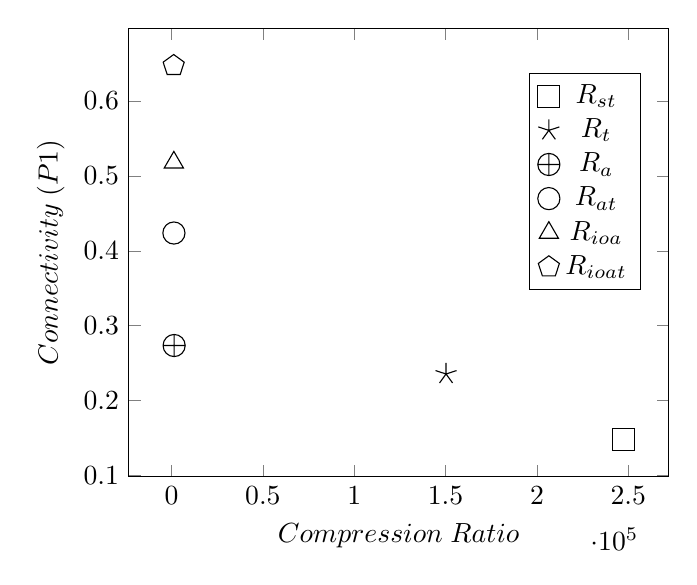
\begin{tikzpicture}
\begin{axis}[
  scatter/classes={
        a={mark=square},%
        b={mark=star},%
        c={mark=oplus},%
        d={mark=o},%
        e={mark=triangle},%
        f={mark=pentagon}
  },
  ylabel=$Connectivity \; (P1)$,
  xlabel=$Compression \; Ratio$,
  mark options={scale=2},
  legend style={at={(.95,0.9)}}
]
\addplot[scatter,only marks,scatter src=explicit symbolic]
coordinates {
% (6.6441, 0.14856667) [a] %0.1301) [a]
% (6.5291, 0.2356) [b] %0.2057) [b]
% (57.4105, 0.2736) [c] %0.2664) [c]
% (65.8846, 0.4238) [d] %0.4221) [d]
% (69.0500, 0.51803333) [e] %0.5169) [e]
% (77.2328, 0.64733333) [f] %0.6598) [f]

(247305.94, 0.14856667) [a]
(150252.41, 0.2356) [b]
(1433.53, 0.2736) [c]
(1314.50, 0.4238) [d]
(1268.24, 0.51803333) [e]
(1184.26, 0.64733333) [f]

};
\legend{$R_{st}$, $R_{t}$, $R_{a}$, $R_{at}$, $R_{ioa}$, $R_{ioat}$}
\end{axis}
\end{tikzpicture}

		}
		\caption{Connectivity precision versus volume ratio.}
		\label{fig:trade-conn-volume}
	\end{subfigure}
	\qquad
	\begin{subfigure}[t]{0.46\textwidth}
		\resizebox{\textwidth}{!}{
			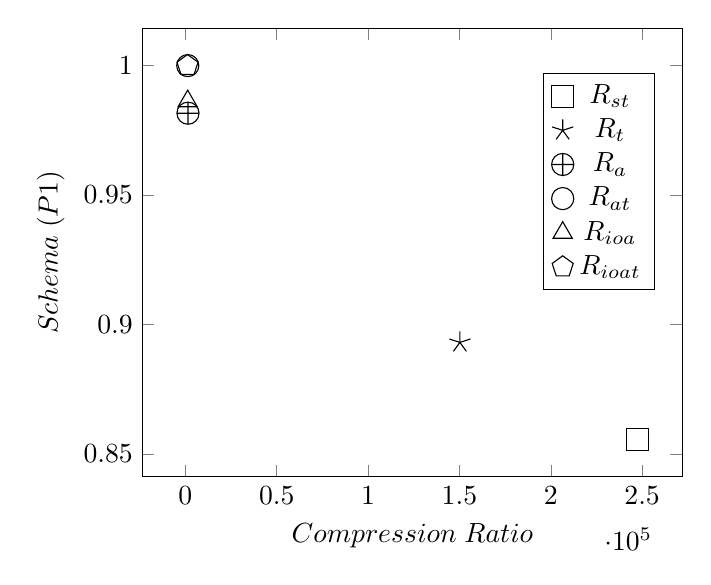
\begin{tikzpicture}
\begin{axis}[
  scatter/classes={
        a={mark=square},%
        b={mark=star},%
        c={mark=oplus},%
        d={mark=o},%
        e={mark=triangle},%
        f={mark=pentagon}
  },
  ylabel=$Schema \; (P1)$,
  xlabel=$Compression \; Ratio$,
  mark options={scale=2},
  legend style={at={(0.95,0.9)}}
]
\addplot[scatter,only marks,scatter src=explicit symbolic]
coordinates {
% (6.6441, 0.85565) [a] %0.6970) [a]
% (6.5291, 0.89303333) [b] %0.8585) [b]
% (57.4105, 0.9816) [c] %0.9733) [c]
% (65.8846, 1.0000) [d]
% (69.0500, 0.98623333) [e] %0.9795) [e]
% (77.2328, 1.0000) [f]

(247305.94, 0.85565) [a]
(150252.41, 0.89303333) [b]
(1433.53, 0.9816) [c]
(1314.50, 1.0000) [d]
(1268.24, 0.98623333) [e]
(1184.26, 1.0000) [f]

};
\legend{$R_{st}$, $R_{t}$, $R_{a}$, $R_{at}$, $R_{ioa}$, $R_{ioat}$}
\end{axis}
\end{tikzpicture}

		}
		\caption{Schema precision versus volume ratio.}
		\label{fig:trade-schema-volume}
	\end{subfigure}
	\qquad%
	\begin{subfigure}[t]{0.46\textwidth}
		\resizebox{\textwidth}{!}{
			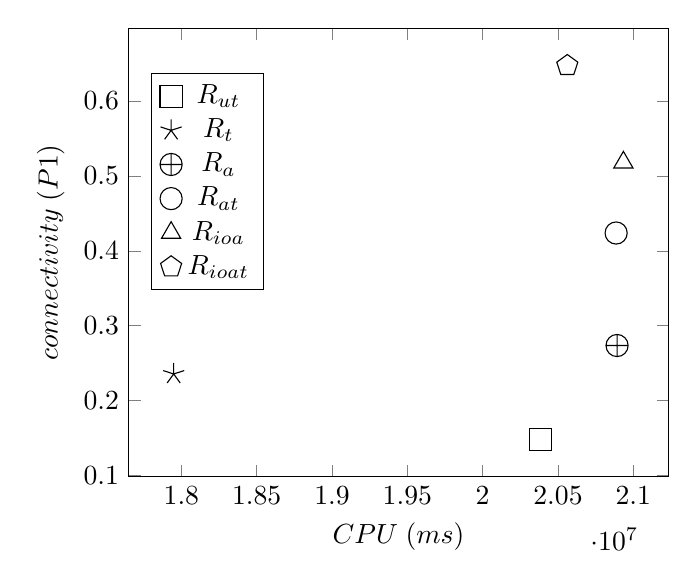
\begin{tikzpicture}
\begin{axis}[
  scatter/classes={
        a={mark=square},%
        b={mark=star},%
        c={mark=oplus},%
        d={mark=o},%
        e={mark=triangle},%
        f={mark=pentagon}
  },
  ylabel=$\gls{connectivity} \; (P1)$,
  xlabel=$CPU \; (ms)$,
  mark options={scale=2},
  legend style={at={(0.25,0.9)}}
]
\addplot[scatter,only marks,scatter src=explicit symbolic]
coordinates {
% (24844125.1190, 0.1301) [a]
% (24669863.0952, 0.2057) [b]
% (24277682.3810, 0.2664) [c]
% (28968841.4286, 0.4221) [d]
% (22053489.7619, 0.5169) [e]
% (22386809.1667, 0.6598) [f]
 (20384066, 0.14856667) [a]
 (17949001, 0.2356) [b]
 (20892062, 0.2736) [c]
 (20885921, 0.4238) [d]
 (20934061, 0.51803333) [e]
 (20561815, 0.64733333) [f]
};
\legend{$R_{ut}$, $R_{t}$, $R_{a}$, $R_{at}$,
 $R_{ioa}$, $R_{ioat}$}
\end{axis}
\end{tikzpicture}

		}
		\caption{Connectivity precision versus summarisation performance.}
		\label{fig:trade-conn-cpu}
	\end{subfigure}
	\qquad%
	\begin{subfigure}[t]{0.46\textwidth}
		\resizebox{\textwidth}{!}{
			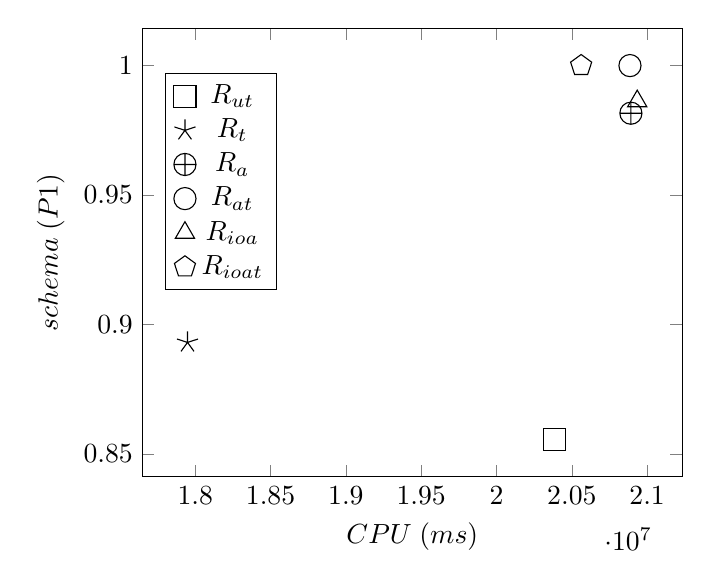
\begin{tikzpicture}
\begin{axis}[
  scatter/classes={
        a={mark=square},%
        b={mark=star},%
        c={mark=oplus},%
        d={mark=o},%
        e={mark=triangle},%
        f={mark=pentagon}
  },
  ylabel=$\gls{schema} \; (P1)$,
  xlabel=$CPU \; (ms)$,
  mark options={scale=2},
  legend style={at={(0.25,0.9)}}
]
\addplot[scatter,only marks,scatter src=explicit symbolic]
coordinates {
% (24844125.1190, 0.6970) [a]
% (24669863.0952, 0.8585) [b]
% (24277682.3810, 0.9733) [c]
%% (28968841.4286, 1.0000) [d]
% (22053489.7619, 0.9795) [e]
% (22386809.1667, 1.0000) [f]

 (20384066, 0.85565) [a]
 (17949001, 0.89303333) [b]
 (20892062, 0.9816) [c]
 (20885921, 1) [d]
 (20934061, 0.98623333) [e]
 (20561815, 1) [f]
};
\legend{$R_{ut}$, $R_{t}$, $R_{a}$, $R_{at}$, $R_{ioa}$, $R_{ioat}$}
\end{axis}
\end{tikzpicture}

		}
		\caption{Schema precision versus summarisation performance.}
		\label{fig:trade-schema-cpu}
	\end{subfigure}
	\caption{Efficiency and precision trade-offs of the candidate summarisation relations. The values are taken as the average across all dataset categories.}
\end{figure}


\section{Graph Summary for Web Data Management}
\label{chap03:sec:wd-mgnt}

The graph summary highlights the structure of a graph, which in the case of RDF data consists in the use of predicates, classes, and their relationships. As such, a graph summary exhibits a similar purpose as a \emph{schema} in relational database management systems. In comparison to the VoID~\cite{alexander:2009:dld} approach, the use of a graph summary as a schema provides additional information, e.g., which predicates co-occur, or how are the classes in a dataset inter-connected.

We define a graph schema model on top of a graph summary in Section~\ref{chap03:sec:gschema}. We describe an RDF model for a graph summary in Section~\ref{chap03:summary-rdf}.

\subsection{Graph Schema}
\label{chap03:sec:gschema}

In order to use the information in a graph effectively, it is necessary to have a schema of that graph. The schema provides a description of the structure of the entity graph. Given a graph schema~\cite{buneman:1997:asu,kunii1983graph}, it is then possible to understand how the data is structured so that it is possible to perform meaningful operations such as querying, optimising query execution, or partitioning data.% \todo{add refs}

The schema of the entity graph is itself a graph as in \cite{kunii1983graph}, where a model for defining integrity constraints and similar rules as in a traditional relational database schema is proposed. In this work, we focus on the structural description of the graph.% We consider the schema as a graph where there is a \emph{simulation} from the entity graph to that schema \cite{wang:2000:ags}. We refer to the schema of the entity graph simply as the \emph{graph schema}. \todo{Review mention of simulation}

\subsection{Overview}

Knowledge is commonly represented using directed graphs, as it is expressive enough for modelling data with complex relationships. For example, semantic networks~\cite{quillan:1966:semantic} have been used in artificial intelligence and machine translation, with the Web of Data being a large scale instance.

Similarly to schemas in databases, there exists \emph{graph schemas} which defines the structure of the graph. A graph schema can be pre-defined as in a top-down approach, or can be generated from the data itself in a bottom-up approach. Thanks to a graph schema, we suspect that the potential benefits are numerous: optimisation of query processing, data integration, data discovery, etc.

There exists two approaches for creating a graph schema, each sitting at opposite ends as depicted by Figure~\ref{fig:introduction:schema-tradeoffs}. On the right side, we have the top-down approaches where a person creates the schema manually. Such a hand-crafted schema ensures the data to be conform with it, but at the cost of less flexibility with regards to the evolution of the schema in time and its customisation to specific needs.

On the left side, we have the bottom-up approaches which rely only on the data. Such schemas offer more flexibility when manipulating the data, but they offer more heterogeneous information.
Indeed, a hand-crafted schema is the result of a careful thought-process, while a generated (bottom-up approach) schema is susceptible to data heterogeneity.

The two approaches highlight a time dimension to the creation of a schema: in the top-down approach, the schema is first created and then the data is produced; in the bottom-up approach instead, this is the opposite: the data is first produced and then a schema is created from it.

\begin{figure}
	\centering
	\resizebox{.6\textwidth}{!}{
		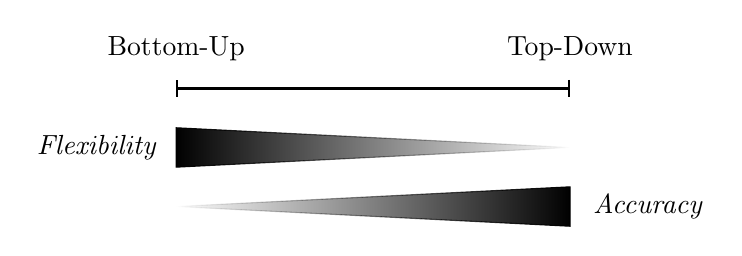
\begin{tikzpicture}
\node (bt) at (0,.5) {Bottom-Up};
\node (td) at (5,.5) {Top-Down};
\draw [|-|,thick] (0,0) -- (5,0);

\node at (-1,-.75) {\emph{Flexibility}};
\draw [fill=black,path fading=east] (0,-.5) -- (5,-.75) -- (0,-1) -- cycle;

\node at (6,-1.5) {\emph{Accuracy}};
\draw [fill=black,path fading=west] (0,-1.5) -- (5,-1.25) -- (5,-1.75) -- cycle;
\end{tikzpicture}

	}
	\caption{Trade-offs between graph schema creation approaches.}
	\label{fig:introduction:schema-tradeoffs}
\end{figure}

\subsubsection{Top-Down Graph Schema}

The structure of the graph can be rigorously defined. In \cite{kunii1983graph} the schema of the database is itself represented as a graph, which facilitates the construction of the database as well as the query formulation. In \cite{antoniou2004web} the authors present the Web Ontology Language which represents the ontology layer in the Semantic Web stack. It allows to define classes, properties, and relationships between classes. Regarding XML data, a graph schema can be expressed via \emph{XML Schemas}\footnote{XMLSchema: \url{http://www.w3.org/XML/Schema}}. In these methods, the graph data either has to be squeezed to fit the pre-defined schema, or the schema has to be updated to meet the new structure of the underlying data. Updating the schema is an expensive operation, since the graph schemas are generally complex.

\subsubsection{Bottom-Up Graph Schema}

In a bottom-up approach, the schema is generated from the data itself by using some features of the data, e.g., attributes of a node. In order to generate a schema, the process must then preserve the \emph{structure} of the graph. %Such a process is called a \emph{graph homomorphism}, i.e., a mapping from the data to the graph schema where every adjacent nodes in the data are mapped to adjacent nodes in the graph schema. The Figure~\ref{fig:introduction:homomorph} depicts a graph that is homomorphic to the graph in Figure~\ref{fig:introduction:graph}, which is then called the \emph{schema} of that graph.
Buneman et. al.~\cite{buneman:1997:asu} defines that a graph dataset conforms to a graph schema if there exists a simulation from the dataset to the graph schema. Informally, whenever there is an edge in the dataset, there is a corresponding edge in the graph schema. 
This can be achieved by using a \gls{summarisation-relation}. Indeed, a graph summary is defined as a graph homomorphism in Section~\ref{sec:summary:model}. As such, we can use a graph summary to fulfill the function of a schema.

%The authors in \cite{goldman1997dataguides} propose \emph{DataGuides}, a method based on automata equivalence which allows to generate a concise and accurate graph schema. However, due to the structural heterogeneity of the graph, the generated graph schema may be large or even larger than the data itself, as discussed in \cite{goldman1999approximate}. In order to counter-balance this, some techniques allow some errors in the graph so to keep the graph schema concise, e.g., \cite{chen:2003:dia,navlakha:2008:gsb}. For example, although the graph in Figure~\ref{fig:introduction:homomorph} shows a path from the node 3 to the node 2 via 1, there is no such path in the graph of Figure~\ref{fig:introduction:graph}.

%\begin{figure}
%	\centering
%	\begin{subfigure}[b]{.4\textwidth}
%		\centering
%		\includegraphics[scale=0.5]{01-introduction/figures/homomorphism1.eps}
%		\caption{A data graph. Nodes within a dashed circle are mapped to a same node.}
%		\label{fig:introduction:graph}
%	\end{subfigure}
%	\quad
%	\begin{subfigure}[b]{.45\textwidth}
%		\centering
%		\includegraphics[scale=.5]{01-introduction/figures/homomorphism2.eps}
%		\caption{A graph homomorphic to the graph in Figure~\ref{fig:introduction:graph}}
%		\label{fig:introduction:homomorph}
%	\end{subfigure}
%	\caption{Graph schema based on a graph homomorphism.}
%\end{figure}

\subsubsection{Graph Schema Granularity}

There is a need for schemas of varying granularity. It is common for database schemas to be large and therefore difficult for users to understand. The authors in \cite{yu:2006:schema-summarization,yang:2011:summary-graphs} proposed methods for summarizing the information in schemas in order to highlight the ``important'' parts. This shows that applications having different degree of interactivity with the data require different parts to be focused, while others can be hidden. We call this notion the \emph{granularity level} of the schema.

%By altering the mappings in the graph homomorphism, the resulting schema is then more or less coarse, i.e., it carries more or less information about the data. For instance in Figure~\ref{fig:introduction:graph}, if the two nodes $a$ and $b$ were mapped to different nodes in the schema, the latter would be finer grained than the schema in Figure~\ref{fig:introduction:homomorph}, since the path from node 2 to 3 via node 1 would not exist.
A varying level of granularity can be achieved by modifying appropriately the \gls{summarisation-relation} of a graph summary. By altering the mappings of the relation, the resulting schema is then more or less coarse, i.e., it carries more or less information about the data. The granularity can be varied through the use of the presented \glspl{summarisation-relation} in Section~\ref{sec:approximate}. How coarse a granularity is can be measured thanks to the graph summary precision model introduced in Chapter~\ref{chap03:sec:quality}.

%\subsection{Abstract Model}
%\label{sec:gschema:abstract-model}
%
%The graph schema is a graph that describes the structure of the entity graph $G$. It informs on the types used, the relations between types, and the attributes associated with a type.
%%The graph schema is a layer located between the entity and the dataset layers. There can be more than one graph schema for a given entity graph, with each providing more or less details about the structure of the entity graph.
%Although the schema is represented as a graph, its elements carry a different semantics than in an entity graph. The reason is that the schema describes the structure of the entity graph. A node in a graph schema represents a \emph{collection} of nodes in the entity graph. Furthermore, it can be associated with attributes and types information, derived from the entities it is composed of. An edge in a graph schema represents a \emph{set} of edges in the entity graph that connect entities together.
%
%\begin{quote}
%	The Figure~\ref{fig:schema-graphs} depicts two possible graph schemas for Figure~\ref{fig:graph}. A node in a graph schema reports on the left column the type, on the right the attribute, and on the bottom row are indicated the entities of the figure it contains.
%	The schema on Figure~\ref{fig:sg1} is minimal, it consists of a single node with all the edges appearing in the entity graph adjacent to it. Although it is a valid graph schema, it does not however give any insight in the entity graph beyond what attributes and what types are used.
%	A deeper insight is achieved with the schema on Figure~\ref{fig:sg2} generated by grouping entities based on their type feature, e.g., we observe that a Person is connected to a City via the link ``lives''.
%\end{quote}
%
%While generating a graph schema, it is possible to gather statistics about the data. For example, we can count the number of entities a node of the schema contains, or how many times a certain attribute is used. The accumulation of such statistics can be used for various purpose, e.g., browsing the most used parts of the data.
%
%\begin{figure}
%	\centering
%	\begin{subfigure}{.42\textwidth}
%		\centering
%		\resizebox{\textwidth}{!}{
%			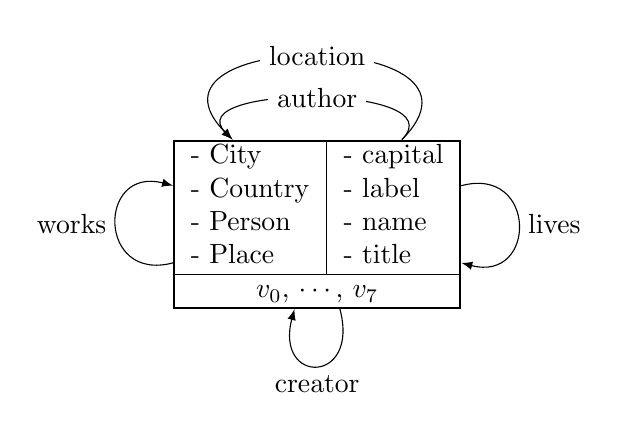
\begin{tikzpicture}[>=latex]
\node (T) [draw,thick,rectangle, inner sep=0pt] {
\begin{tabular}{l|l}
- City & - capital \\
- Country & - label \\
- Person & - name \\
- Place & - title \\
\hline
\multicolumn{2}{c}{$v_0$, $\cdots$, $v_7$}
\end{tabular}
};
\draw [loop, distance=2cm,->] (T) to node [fill=white] {location} (T);
\draw [loop, distance=1cm,->] (T) to node [fill=white] {author} (T);
\draw [loop below, distance=1cm,->] (T) to node {creator} (T);
\draw [loop right, distance=1cm,->] (T) to node {lives} (T);
\draw [loop left, distance=1cm,->] (T) to node {works} (T);
\end{tikzpicture}
%		}
%		\caption{A simple graph schema}
%		\label{fig:sg1}
%	\end{subfigure}
%	\quad
%	\begin{subfigure}{.54\textwidth}
%		\centering
%		\resizebox{\textwidth}{!}{
%			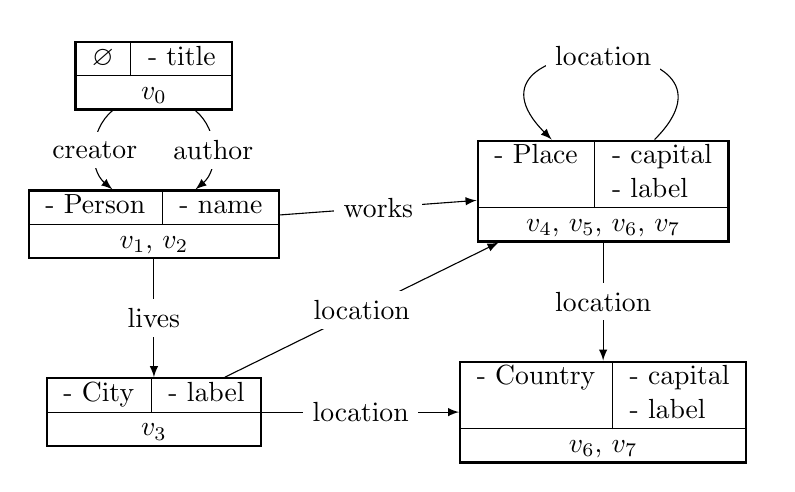
\begin{tikzpicture}[>=latex]
\node (city) [draw,thick,rectangle,inner sep=0] {
\begin{tabular}{l|l}
- City & - label \\
\hline
\multicolumn{2}{c}{$v_3$}
\end{tabular}
};
\node (country) [draw,thick,rectangle,inner sep=0, right = 2.5cm of city] {
\begin{tabular}{l|l}
- Country & - capital \\
 & - label \\
\hline
\multicolumn{2}{c}{$v_6$, $v_7$}
\end{tabular}
};
\node (person) [draw,thick,rectangle,inner sep=0,above = 1.5cm of city] {
\begin{tabular}{l|l}
- Person & - name \\
\hline
\multicolumn{2}{c}{$v_1$, $v_2$}
\end{tabular}
};
\node (place) [draw,thick,rectangle,inner sep=0,above =1.5cm of country] {
\begin{tabular}{l|l}
- Place & - capital \\
 & - label \\
\hline
\multicolumn{2}{c}{$v_4$, $v_5$, $v_6$, $v_7$}
\end{tabular}
};
\node (pub) [draw,thick,rectangle,inner sep=0,above = of person] {
\begin{tabular}{l|l}
$\varnothing$ & - title \\
\hline
\multicolumn{2}{c}{$v_0$}
\end{tabular}
};

\draw [->] (person) to node [fill=white] {lives} (city);
\draw [->] (person) to node [fill=white] {works} (place);
\draw [->] (city) to node [fill=white] {location} (place);
\draw [->] (city) to node [fill=white] {location} (country);
\draw [->] (place) to node [fill=white] {location} (country);
\draw [loop,distance=2cm,->] (place) to node [fill=white] {location} (place);
\draw [bend left=50,->] (pub) to node [fill=white] {author} (person);
\draw [bend right=50,->] (pub) to node [fill=white] {creator} (person);

\end{tikzpicture}
%		}
%		\caption{A graph schema based on the \emph{Types} summarisation relation $R_t$}
%		\label{fig:sg2}
%	\end{subfigure}
%	\caption{Two possible graph schemas for Figure~\ref{fig:graph}. The left columns report the type information of a node, while the right the attribute. The bottom row of a node indicates the entities of the figure it contains.}
%	\label{fig:schema-graphs}
%\end{figure}
%
%\subsection{Formal Model}
%\label{sec:gschema:formal-model}
%
%A graph schema is a graph where there is a \emph{simulation} from the entity graph to that graph schema \cite{wang:2000:ags}. In other words, every path and combination of paths that appear in the entity graph must also appear in the graph schema.
%
%\begin{quote}
%	For example, the entity graph in Figure~\ref{fig:graph} depicts the node $v_1$ of type Person that has three attributes, i.e., lives, name, and works. Both graph schemas in Figure~\ref{fig:schema-graphs} show such a pattern.
%\end{quote}
%
%Each node of the entity graph is mapped to a node in the graph schema; we say then that the entity graph is \emph{simulated by} the graph schema.
%
%\begin{definition}[Simulation]
%	Let $G_1 = \left\langle V_1, A_1, l_{v_1} \right\rangle$ and $G_2 = \left\langle V_2, A_2, l_{v_2} \right\rangle$ be two graphs. A relation $R$ from $V_1$ to $V_2$ is a simulation if it satisfies
%	\begin{equation*}
%	\begin{split}
%	& \forall \alpha \in A_1,\: \forall (x_1,y_1) \in V^2_1,\: \forall x_2 \in V_2 \\
%	&\begin{aligned}
%	\left(x_1 \overset{\alpha}{\rightarrow} y_1 \wedge x_1 R x_2 \implies \exists y_2 \in V_2 \left( y_1 R y_2 \wedge x_2 \overset{\alpha}{\rightarrow} y_2 \right) \right)
%	\end{aligned}
%	\end{split}
%	\end{equation*}
%	\label{eq:simulation}
%\end{definition}
%
%For a relation $R$ to be a \emph{simulation} from the nodes of the graph $G_1$ to $G_2$, it is required that for all edges in $G_1$, there exists a corresponding edge in $G_2$. The Figure~\ref{fig:simulation} depicts the Definition~(\ref{eq:simulation}). The dotted arrows represent the missing requirements for $R$ to be a simulation:
%\begin{enumerate}
%	\item there exists an edge labelled $\alpha$ that links $x_2$ to $y_2$; and
%	\item there is a $R$ relation between the nodes $y_2$ and $y_1$.
%\end{enumerate}
%The definition presents a recursive aspect. The recursion is stopped if a leaf node is met, since two leaf nodes are in simulation. For example in Figure~\ref{fig:simulation}, if the nodes $y_1$ and $y_2$ were literals in the RDF modelling, then there would be a simulation relation between $x_1$ and $x_2$ since both have an attribute $\alpha$ that lead to a leaf node.
%
%A graph schema is \emph{valid} with regards to the entity graph if there exists a simulation from the nodes of the entity graph to those of the graph schema.
%
%\begin{figure}
%	\centering
%	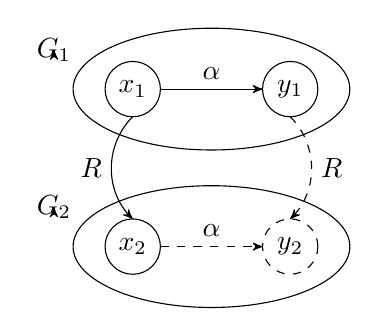
\begin{tikzpicture}[->,>=stealth']
% G1
\draw (2,3) ellipse (50pt and 22pt);
\draw (0,3.5) node {$G_1$};

\draw (1,3) circle (10pt);
\node (x1) at (1,3) {$x_1$};

\draw (3,3) circle (10pt);
\node (y1) at (3,3) {$y_1$};

\draw [->] (1.35,3) -- node[auto]{$\alpha$} (2.65,3);

% G2
\draw (2,1) ellipse (50pt and 22pt);
\draw (0,1.5) node {$G_2$};

\draw (1,1) circle (10pt);
\node (x2) at (1,1) {$x_2$};

\draw (3,1) circle (10pt) [dashed];
\node (y2) at (3,1) {$y_2$};

\draw [dashed,->] (1.35,1) -- node[auto]{$\alpha$} (2.65,1);

% simulation
\draw [->] (1,2.65) to [bend right=45] node[swap,auto]{$R$} (1,1.35);

\draw [->,dashed] (3,2.65) to [bend left=45] node[auto]{$R$} (3,1.35);

\end{tikzpicture}
%	\caption{Depiction of the simulation Definition~(\ref{eq:simulation}).}
%	\label{fig:simulation}
%\end{figure}

%\subsection{Schema Accuracy}
%
%A graph schema describes the structure of the entity graph. From the simulation relation, we know that any path occurring in the data appears in the schema as well. However, the opposite may not always be true. It is possible to draw some conclusions about the data by observing the schema that may actually be wrong. By wrong, we mean that a graph pattern occurs in the schema, but not in the data. This generally stems from the data heterogeneity, i.e., a loose use of a variety of vocabularies.
%
%The schema graph in Figure~\ref{fig:sg2} depicts two nodes, one with type \emph{Place} and the other with \emph{Country}. For both, it reports \emph{capital} and \emph{label} as attributes. However, there is no entity in the data depicted in Figure~\ref{fig:graph} of either type that have both attributes. The reason is that both nodes represent the aggregation of several entities, i.e., $v_4$, $v_5$, $v_6$, and $v_7$ for the one typed \emph{Place}, and $v_6$, $v_7$ for the other.

\subsection{Representation of Graph Summaries}
\label{chap03:summary-rdf}

In this section, we present an RDF model for describing a graph summary. This allows the summary to be queried as any other RDF graph, ultimately so it can be used in conjunction with the entity graph.

Viewing the graph summary as an RDF graph requires the creation of URIs for identifying sumnodes and sumedges. A URI for a sumnode can be created based on the features the \gls{summarisation-relation} it is based on, e.g., on the type information for the \emph{Types} summary $R_t$. The sumedge URI can be created by considering the source and target sumnodes, as well as the attribute.

\begin{remark}
	Although an edge is represented with a single statement in RDF, this is not the case for a sumedge of the summary if we need to associate with it metadata, e.g., statistics or the sumedge provenance. Therefore, we need to describe formally the sumedge.

	For example, consider the sumedge ``\emph{:Person :writes :Book .}'', represented as a triple, which relates the sumnode ``:Person'' to the sumnode ``:Book''. If we need to associate a statistic to that sumedge, we need to RDFify it with four triples:
	\begin{enumerate}
		\item \emph{:se :source :Person .}
		\item \emph{:se :target :Book .}
		\item \emph{:se :label :writes .}
		\item \emph{:se :statistic "1" .}
	\end{enumerate}
	where ``:se'' is the URI for that sumedge, the first triple describes the source, the second the target, the third the label of the sumedge, and the fourth the statistic associated to that triple.
\end{remark}

We depict in Figures~\ref{fig:rdf-node}~and~\ref{fig:rdf-edge} the ontology of the summary RDF model of the sumnode and sumedge respectively, where the label of a node indicates the type of that node. For example, the range of the origin predicate is \emph{xsd:anyURI}. In Figure~\ref{fig:rdf-node} the dot represents an intermediate node, which can be translated into a blank node in the RDF model. We describe in the Table~\ref{tab:rdf-terms} the vocabulary terms.\\

In the case where a summary describes a collection of inter-linked datasets, we record the provenance of the summarised edges at the sumnode (resp., sumedge) level using the predicate \emph{origin}. The predicate \emph{label} indicates the type or attribute associated to a sumnode (resp., sumedge). We record the features of the \gls{summarisation-relation}, e.g., a type for the \emph{Types} summary $R_t$, using the predicate \emph{feature}. In case of a \gls{summarisation-relation} that is based on the type feature, we record as well the attribute type that defined that type.

%\subsubsection{Reification of the sink sumnode $\varnothing$.}

%We present two approaches for reifing the sink sumnode $\varnothing$ (Definition~\ref{def:sink-sumnode}) which represents abstracted data from the entity graph, e.g., literals and URIs with no outgoing edge. With the full reification, we represent it in the RDF summary as an empty literal. Another solution would be to not represent it at all.

\begin{figure}
	\centering
	\begin{subfigure}[b]{.45\textwidth}
		\centering
		\resizebox{\textwidth}{!}{
			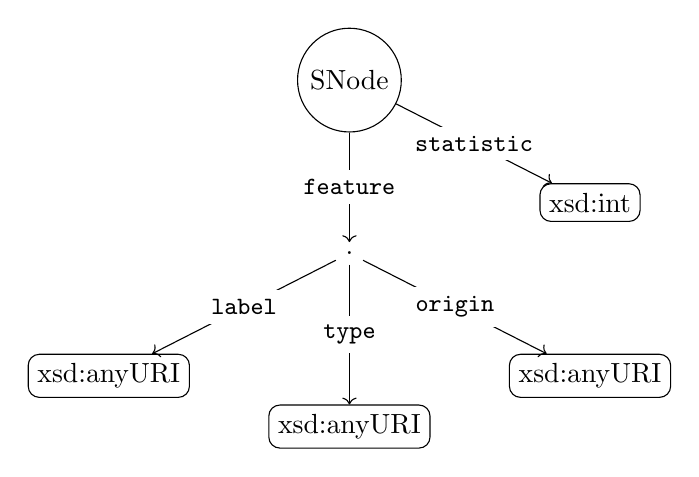
\begin{tikzpicture}[->,node/.style={draw,circle},leaf/.style={draw,rounded corners},node distance=2.2cm]

\node[node] (node) {SNode};
\node[leaf,below right of = node,xshift=1.5cm] (card) {xsd:int};
\node[below of = node] (type) {.};
\node[leaf,below left of = type,xshift=-1.5cm] (typelabel) {xsd:anyURI};
\node[leaf,below right of = type,xshift=1.5cm] (torigin) {xsd:anyURI};
\node[leaf,below of = type] (ttype) {xsd:anyURI};

\path[every node/.style={font=\small\ttfamily,fill=white}]
(node)	edge node {statistic} (card)
			edge node {feature} (type)
(type)	edge node {label} (typelabel)
			edge node {origin} (torigin)
			edge node {type} (ttype)
;
\end{tikzpicture}
		}
		\caption{Node class}
		\label{fig:rdf-node}
	\end{subfigure}
	\quad
	\begin{subfigure}[b]{.35\textwidth}
		\centering
		\resizebox{\textwidth}{!}{
			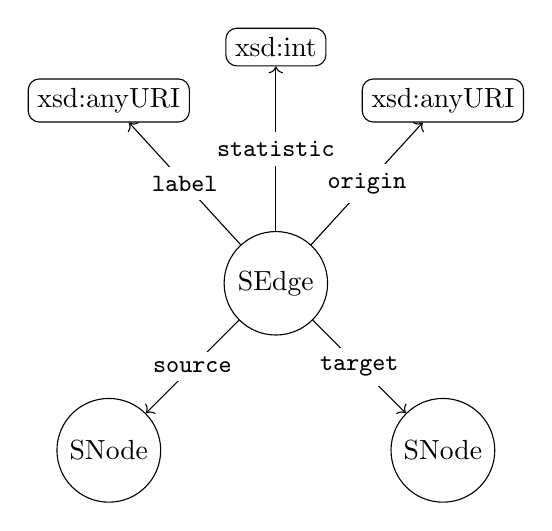
\begin{tikzpicture}[->,node/.style={draw,circle},leaf/.style={draw,rounded corners},node distance=3cm]

\node[node] (edge) {SEdge};
\node[node,below left of = edge] (source) {SNode};
\node[node,below right of = edge] (target) {SNode};
\node[leaf,above left of = edge,yshift=.2cm] (label) {xsd:anyURI};
\node[leaf,above of = edge] (card) {xsd:int};
\node[leaf,above right of = edge,yshift=.2cm] (origin) {xsd:anyURI};

\path[every node/.style={fill=white,font=\small\ttfamily}]
(edge)	edge node {source} (source)
			edge node {target} (target)
			edge node {label} (label)
			edge node {statistic} (card)
			edge node {origin} (origin)
;
\end{tikzpicture}
		}
		\caption{Edge class}
		\label{fig:rdf-edge}
	\end{subfigure}
	\qquad
	\begin{subfigure}[b]{\textwidth}
		\resizebox{\textwidth}{!}{
			\begin{tabular}{lc@{\hs}l}
				\toprule
				& \phantom{a} & \multicolumn{1}{c}{Description} \\
				\cmidrule{3-3}
				\underline{\textbf{Class}} & & \\
				SEdge & \phantom{a} & This class refers to a sumedge $(x, \alpha, y) \in \mathcal{B}$ of the summary. \\
				SNode & \phantom{a} & This class refers to a sumnode $x \in \mathcal{W}$ of the summary. \\
				\midrule
				\underline{\textbf{Predicate}} & & \\
				feature & \phantom{a} & A feature of the \gls{summarisation-relation}. \\
				label & \phantom{a} & The label associated with a sumnode or a sumedge, i.e., either an attribute or a type. \\
				origin & \phantom{a} & The provenance of the summarised edge, or of a feature of the \gls{summarisation-relation}. \\
				source & \phantom{a} & The sumnode $x$ in the sumedge $(x, \alpha, y) \in \mathcal{B}$. \\
				statistic & \phantom{a} & A statistic associated with a sumnode or a sumedge, e.g., \emph{count}. \\
				target & \phantom{a} & The sumnode $y$ in the sumedge $(x, \alpha, y) \in \mathcal{B}$. \\
				type & \phantom{a} & The attribute type \glssymbol{atype}. \\
				\bottomrule
			\end{tabular}
		}
		\caption{Vocabulary terms}
		\label{tab:rdf-terms}
	\end{subfigure}
	\caption{RDF reification of the graph summary}
	\label{fig:rdf-summary}
\end{figure}

\subsubsection{Levels of Reification}

Depending on the use of the graph summary, a subset of the presented vocabulary is needed. For example, if no statistic was computed then the predicate \emph{statistic} is not needed. In this section, we present two possible reifications. A \emph{lite} reification which reifies only the structural information in the summary, and a \emph{full} reification which captures all the information made available by the graph summary.

\minisec{Full Reification}

In this level of reification, we use all vocabulary terms presented in the previous section. We note nonetheless that the \emph{origin} predicate is optional, since it is not needed for summarising a single dataset.\\

Due to the RDF reification of the summary, there exists a case which might cause the summary to be larger than the original. Indeed, if the \gls{summarisation-relation} is a \emph{one-to-one} mapping from the entity graph to the summary, the number of RDF statements used to describe the summary might be greater than for the entity graph. A single statement in the entity graph requires six statements for describing the corresponding sumedge, i.e., the five triples depicted in the Figure~\ref{fig:rdf-edge} plus one for the type attribute.

In addition to those six statements, we must also account for the statements describing the adjacent sumnodes. Depending on the application of the graph summary, the full description of the graph summary can be excessive.\\

Table~\ref{tab:reification-edge-case-full} reports the \emph{Types} summarisation of a simple entity graph for which the summarisation has a one-to-one mapping. We observe that the full reification of the summary consists of 18 triples, against 3 for the entity graph.

\minisec{Lite Reification}

For this reification, we don't retain information such as provenance or statistics. Instead, we are only concerned with the structural description of the graph. A direct consequence is that the size of the RDF summary is reduced significantly. In order to do so, we only need to create a URI for the sumnodes through object invention~\cite{hull:1989:usi}.

Although this reification is not as insightful as the previous one, it provides nonetheless a succinct description of the structure of the graph. Table~\ref{tab:reification-edge-case-lite} reports the lite reification of the graph.

\begin{table}
	\centering
	\begin{subfigure}{.475\textwidth}
		\centering
		\resizebox{\textwidth}{!}{
			\begin{tabular}{lllc@{\s}lll}
				\toprule
				\multicolumn{3}{c}{$G$} & \phantom{a} & \multicolumn{3}{c}{\glssymbol{typessummary}} \\
				\cmidrule{1-3} \cmidrule{5-7}
				\multirow{6}{*}{p1} & \multirow{6}{*}{\glssymbol{atype}} & \multirow{6}{*}{Person} & \multirow{6}{*}{\phantom{a}} & t1 & $a$ & SNode \\
				& & & & t1 & statistic & 1 \\
				& & & & t1 & feature & fp1 \\
				& & & & fp1 & label & Person \\
				& & & & fp1 & type & \glssymbol{atype} \\
				& & & & fp1 & origin & acme.org \\
				\cmidrule{1-3} \cmidrule{5-7}
				\multirow{6}{*}{p1} & \multirow{6}{*}{author} & \multirow{6}{*}{d1} & \multirow{6}{*}{\phantom{a}} & e1 & $a$ & SEdge \\
				& & & & e1 & label & author \\
				& & & & e1 & statistic & 1 \\
				& & & & e1 & origin & acme.org \\
				& & & & e1 & source & t1 \\
				& & & & e1 & target & t2 \\
				\cmidrule{1-3} \cmidrule{5-7}
				\multirow{6}{*}{d1} & \multirow{6}{*}{\glssymbol{atype}} & \multirow{6}{*}{Document} &\multirow{6}{*}{\phantom{a}} & t2 & $a$ & SNode \\
				& & & & t2 & statistic & 1 \\
				& & & & t2 & feature & fp2 \\
				& & & & fp2 & label & Document \\
				& & & & fp2 & type & \glssymbol{atype} \\
				& & & & fp2 & origin & acme.org \\
				\bottomrule
			\end{tabular}
		}
		\caption{Full reification. The edge $(p1, author, d1)$ is mapped to the sumedge that is reified with \emph{e1}.}
		\label{tab:reification-edge-case-full}
	\end{subfigure}
	\quad
	\begin{subfigure}{.475\textwidth}
		\centering
		\resizebox{\textwidth}{!}{
			\begin{tabular}{lllc@{\s}lll}
				\toprule
				\multicolumn{3}{c}{$G$} & \phantom{a} & \multicolumn{3}{c}{\glssymbol{typessummary}} \\
				\cmidrule{1-3} \cmidrule{5-7}
				p1 & \glssymbol{atype} & Person & \phantom{a} & t1 & \glssymbol{atype} & Person \\
				p1 & author & d1 & \phantom{a} & t1 & author & t2 \\
				d1 & \glssymbol{atype} & Document & \phantom{a} & t2 & \glssymbol{atype} & Document \\
				\bottomrule
			\end{tabular}
		}
		\caption{Lite reification.}
		\label{tab:reification-edge-case-lite}
	\end{subfigure}
	\caption[Full and lite reification of a \emph{Types} summary $R_t$]{Full and lite reification of a \emph{Types} summary $R_t$. The summarisation relation $R_t$ has with the example data a one-to-one mapping from the graph $G$ to the summary \glssymbol{typessummary}. The node \emph{p1} is mapped to the sumnode \emph{t1} and \emph{d1} to \emph{t2}.}
	\label{tab:reification-edge-case}
\end{table}

%\subsection{Deploying Graph Summaries}
%\label{chap03:summary-deploy}

%In order to deploy a graph summary, we embed it into a named graph which is preferably located in the same endpoint as the entity graph. In this way, the summary can be used in conjunction with the original data.


%%
%% tree ranking
%%
\chapter{Tree Ranking}
\label{chap:tree-ranking}

The Web of Data can be seen as an encyclopaedia spanning over the entire Web. It contains rich information about concrete and abstract things covering a variety of domains, e.g., people, organisations, companies, media such as music or films, geographical places of interest. In Web Data, each of these is referred to as an \emph{entity} to which is associated structured data, e.g., the name of a person or the description of a country.

The amount of entities on the Web that are associated with a structured description has reached a state where the search for specific entities can only be handled with systems such as web search engines. These systems are based on the Information Retrieval (IR) paradigm. Moreover, entities present a high structural heterogeneity which cannot be handled by traditional relational databases. Indeed, entities from a same domain can have a completely different set of descriptive attributes, or use attributes that don't reflect the data the best. In this chapter, we investigate the ranking of entities for IR search engines.

Current IR engines are not adapted to the structural heterogeneity of entities. In web search engines, field-based ranking models are popular for the ranking of structured documents such as HTML pages. However, fields need to be known a priori and the fact that a same entity can have multiple values for a same attribute is not considered. We introduce in this chapter an extension to field-based ranking models which addresses these shortcomings and that fits to arbitrarily-shaped entities.

\section{Related Work}
\label{sec:searching:relwork}

The Web of Data consists of a wide range of heterogeneous datasets, where the schema and the ontology can vary from one to the other. To overcome this diversity of attributes, different approaches for defining the fields of an entity have been proposed.\\

From an RDF perspective, the authors consider in \cite{Perez-Aguera:2010:UBS} five weighted fields to represent the structure of an entity: literals (textual values), keywords extracted from the root's label, i.e., the subject URI, keywords extracted from the incoming links, the entity's types and keywords extracted from object URIs. Compared to the BM25F and PL2F field-based approaches defined in \ref{sec:ranking-wod}, this approach is not able to grasp the rich structure of the data since attributes are discarded.

The BM25F and PL2F approaches we use in our experiments Section~\ref{sec:experiments} are similar in nature to the BM25F adaptation proposed in \cite{blanco:2011:iswc}, where the authors consider one field per attribute in the data collection and can assign a different weight to each attribute. However, they restrict their approach to attributes with literal values, discarding those with URI values. In contrast to \cite{blanco:2011:iswc}, we consider attributes both with literal and URI values. URIs in an RDF graph carry relevant keywords, with regards to
\begin{inparaenum}[(1)]
	\item the entity in general when considering the subject URI;
	\item the attribute when considering the predicate URI; and
	\item the related entity when considering the object URI.\\
\end{inparaenum}
%We also consider in our approach the entity and the attribute labels, i.e., the predicate URIs, using special entity attributes. This aspect is discussed in the Section~\ref{sec:with-att}.

However, all these approaches are an adaptation of the field-based ranking model in which multiple values associated to a same attribute are aggregated into a single value. This simplification of the underlying data model is inadequate for structured data. Therefore, we propose an extension of field-based ranking models in Section~\ref{chap:tree-ranking:mf-model} to take into consideration multi-valued attributes and show that our model can be effectively applied to different ranking frameworks.

%\chapter{Ranking of (Semi-)Structured Data}
%
%At its beginning, The Internet was a collection of hypertext documents: textual data with links to additional textual data. At first, search engines were focused on retrieving documents, but with the growth of The Internet, a need for \emph{ranking} documents with regards to how important they are regarding a user's query appeared. Documents consisting only of text, the ranking models assumed as much and no structural information was considered. Nonetheless, some structural cues could still be extracted from the documents, e.g., title, paragraphs, links, \ldots, thanks to the HTML markup are written in. Including these cues into the ranking model improved noticeably its performance.
%
%With the coming of the Semantic Web, documents are turning into a real blend of structured and unstructured data. The structural information is clearly defined. Since this marked a shift of how documents are modelled, there was a need for ranking models to adapt. In this chapter, we present some ranking models used over (semi-)structured data, and introduce the ranking model used in this thesis as a basis for Chapter~\ref{chap:tree-ranking}.
%
%\section{Traditional Ranking Models}
%
%\section{Abstract Model}
%
%\section{Formal Model}

%\section{Entity Model}
%\label{chap:entity-ranking:entity-model}
%
%In this section, we define what is an entity, i.e., the unit of information that is queried and retrieved by an IR search engine. The entity model is based on the graph model presented in Section~\ref{sec:gdm:formal-model}.% In this chapter, we use \emph{document} as an equivalent term for \emph{entity}, since a document is the common term for the object that is ranked in an IR search engine.
%
%An entity in a graph data model is defined as a sub-graph in which a node is considered as the \emph{root}. In RDF the root is the URI that represents that entity, e.g., the URI \url{http://dbpedia.org/page/Earth} for referring to the planet Earth. The edges related to that root form then what we call an \emph{entity}.
%
%\begin{definition}[Entity]
%Let $G = \left\langle V, A, l_V \right\rangle$ be a graph. We call an entity rooted in $u \in V$ a sub-graph of $G$ in which the edges and nodes are a related to the root $u$.
%\end{definition}
%
%There exist several ways to define which edges are related to a root node. We can consider the entity as the connected component that emerges from that root. This can be achieved by performing a breadth-first search starting at the root, and adding the traversed edges and nodes to the entity. Also, one may consider a set of unconnected sub-graphs as the entity according to a similarity measure.
%
%In this chapter, we use the approach described in~\cite{delbru:jws:entity}, where an entity is a star graph, i.e., a sub-graph with a node (the root) and its direct neighbouring nodes it links to. The Figure~\ref{fig:rdf-graph} displays how a graph can be split into four entities \emph{me}, \emph{\_:b1}, \emph{\_:b2} and \emph{paper/547}. Each entity forms a sub-graph containing the incoming and outgoing edges of the root node. In order to simplify the extraction process, we only consider the outgoing edges of a root node.

%\subsubsection{Entity Model}
%
%In the remainder of the paper, the unit of information which is retrieved and ranked is an \emph{entity}~\cite{delbru:jws:entity} and is formalised as a list of attribute-value pairs:
%\begin{description}
%  \item[Entity] represents a set of attribute-value pairs and is identified by the entity node label, e.g., \emph{paper/547};
%  \item[Attribute] is an edge linking the entity node to one of its neighbour nodes and is identified by the edge label, e.g., \emph{title}, \emph{name} or \emph{creator};
%  \item[Value] is a neighbour node of the entity node and is identified by the node label, e.g., \emph{Object-} or \emph{paper/547}. A value is always associated to one attribute. Multiple values can be associated to a same attribute, such as the nodes \emph{\_:b1} and \emph{\_:b2} with the attribute \emph{knows} of the entity \emph{me}.
%\end{description}
%
%\begin{figure}
%	\centering
%	\resizebox{0.65\textwidth}{!}{
%		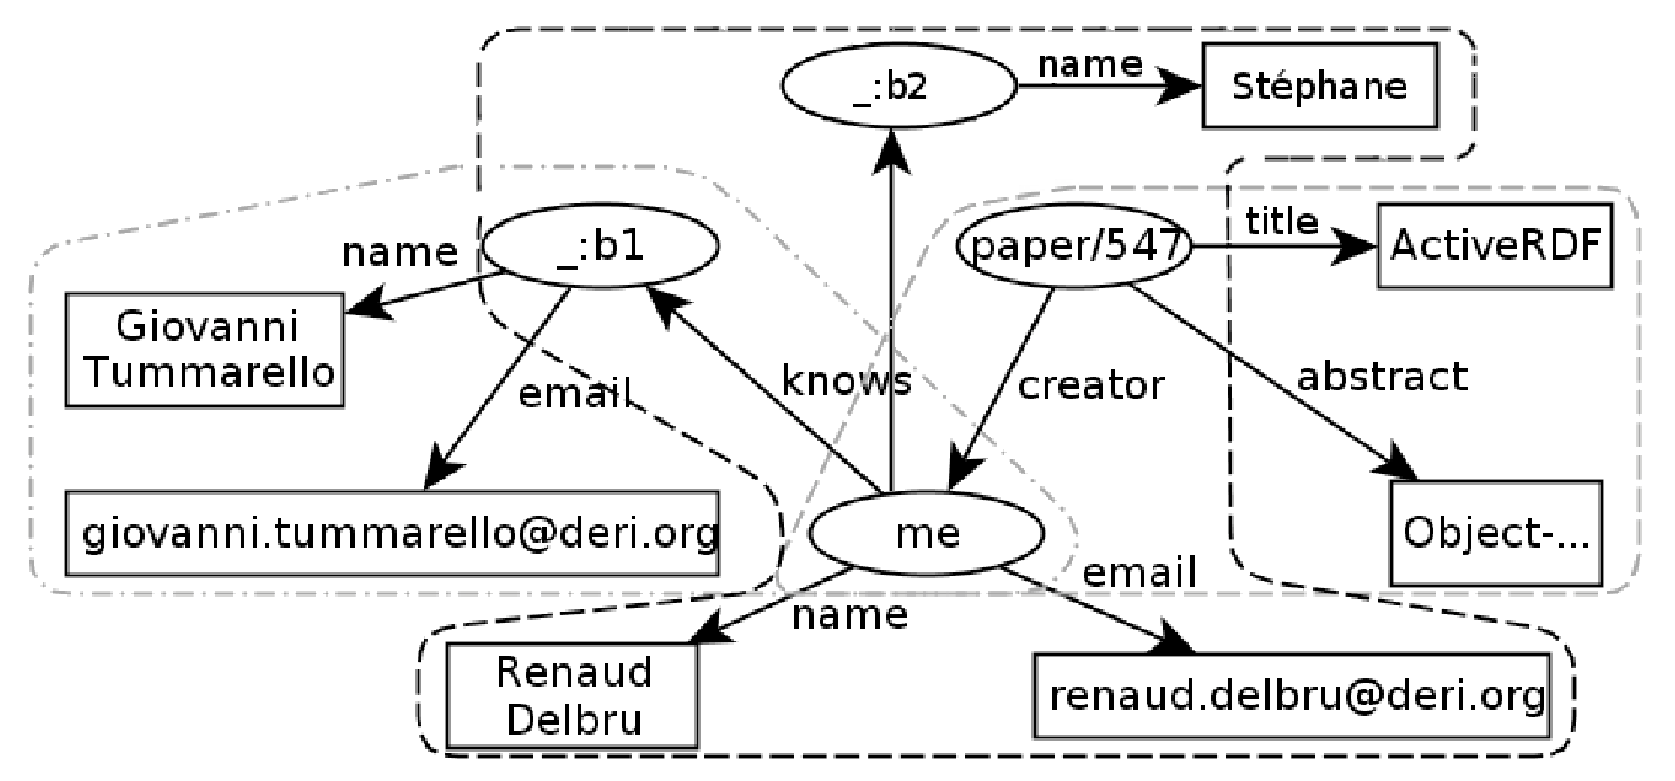
\includegraphics[scale=1]{05-ranking/figures/rdf-graph}
%	}
%	\caption{A graph divided into four entities identified by the root nodes \emph{me}, \emph{\_:b1}, \emph{\_:b2} and \emph{paper/547}.}
%	\label{fig:rdf-graph}
%\end{figure}

\section{Ranking Model Foundations}

We describe in this section vocabulary terms that will be reused throughout this chapter. We consider here a dataset to be a collection of entities, each entity being a graph. An entity may represent a person, a place, or an organisation. The \emph{unit of information} which is retrieved and ranked is an entity.

We consider an entity to be a graph centered around a node, that we call the root, where each edge provides some description of that node. We define a rooted entity as the \emph{entity description} (Definition~\ref{def:entity-description}) of a \emph{root} node, where every node in the entity description is reachable from that root node.

\begin{definition}[Rooted Entity]
Let $G = \left\langle V, A, l_V \right\rangle$ be a graph, and let $\glssymbol{edesc}(u \in V) \subseteq A$ be the entity description of the node $u$. We call the entity description \glssymbol{edesc}(u) a rooted entity in $u$ if and only if there is a path from $u$ to every node in $\glssymbol{edesc}(u)$.
\end{definition}

Figure~\ref{fig:entities} depicts four entities identified by the root nodes \emph{me}, \emph{\_:b1}, \emph{\_:b2} and \emph{paper/547}.

\begin{figure}
	\centering
	\resizebox{0.65\textwidth}{!}{
		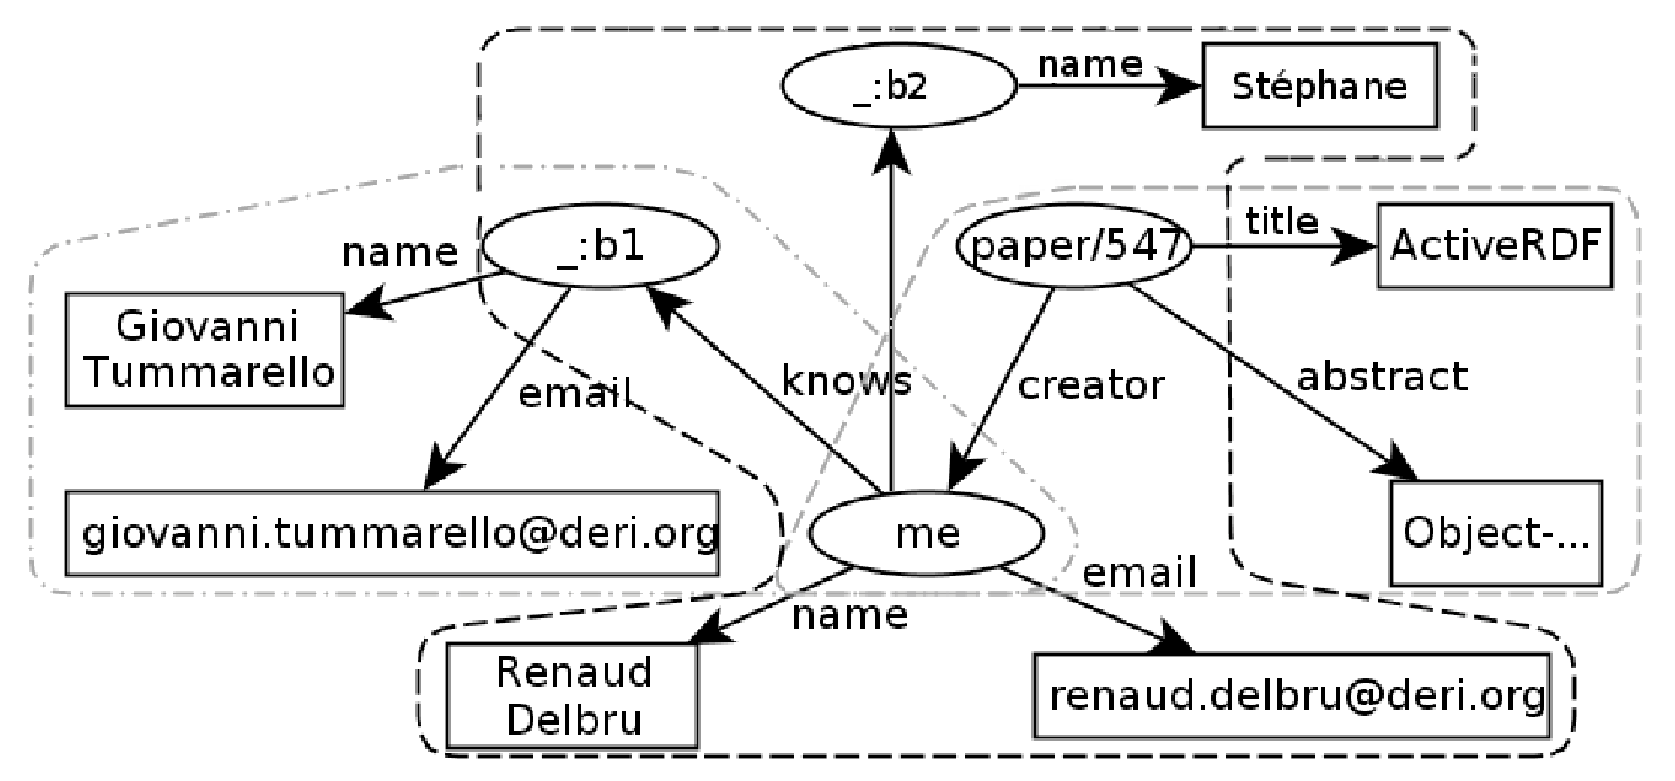
\includegraphics[scale=1]{05-ranking/figures/rdf-graph}
	}
	\caption{A graph divided into four entities identified by the root nodes \emph{me}, \emph{\_:b1}, \emph{\_:b2} and \emph{paper/547}.}
	\label{fig:entities}
\end{figure}

We define here some vocabulary used in the rest of the chapter:
\begin{description}
	\item[term:] a node label can be split over some character, e.g., a white space; we refer to a token resulting from this operation a \emph{term}.
	\item[length:] the length denotes the number of terms, e.g., in a node.
\end{description}

\section{Field-Based Ranking Models}
\label{sec:ranking-wod}

In this section, we explain how to adapt two existing field-based ranking frameworks to the graph model described in Chapter~\ref{chap:ssd}.
A field-based ranking model views a graph as composed of multiple normalized weighted fields. For example, a field can be the title, the author or the body of the document.\\

In the Probabilistic Relevance Framework~\cite{Robertson:2009:PRF} (PRF), BM25F~\cite{zaragoza:2004:microsoft} is a field-based ranking function popular for web search.
The Divergence From Randomness~\cite{amati:2002:acm} (DFR) framework gives birth to many ranking models, in particular to PL2F~\cite{macdonald:2005:clef} which is of the field-based family.\\

In field-based ranking approaches, different parts of the entity description are arranged into various categories that we denote as \emph{fields}. A field is then composed of field labels and/or edge labels. A \emph{score} of the entity is computed to reflect how relevant the entity is with regards to a query; the score computation is dependent of the fields.

In presence of a multi-valued attribute, the common approach is to merge the content of all the values into one single value.

\minisec{Ranking Features}

The following features are used in the field-based ranking functions:
\begin{labeling}{\textbf{average field length}}
	\item[\textbf{field length}] refers to the number of terms in a node label. In case of a multi-valued fields, it refers to the number of terms across all the nodes associated with the field.
	\item[\textbf{average field length}] is equal to the mean of \emph{field length} across entities.
\end{labeling}

\minisec{Normalised Term Frequency}

The ranking models presented here are from the \emph{TF-IDF} family, where \emph{TF} is a function of the term frequency, and \emph{IDF} is a function of inverse document frequency.

The intuition behind TF is that it captures the relevancy of a term within a graph, e.g., the more a term occurs in a graph, the more important it is for that graph.

In contrary, the intuition behind IDF is to capture the importance of a term within the dataset: the more a term occur in the dataset, the less relevant it is. For example, the term ``food'' would occur frequently in a cooking recipes book, however it may not be an interesting feature in a ranking function.\\

In general, the term frequency is not used ``as is'' in the TF function: it is first \emph{normalised} before applying the TF function. Term frequency normalisation is useful in cases where the length of a graph varies across the dataset: it allows to capture this variability into the ranking function, making the score of entities description comparable. In field-based ranking functions, the term frequency is normalized at the field level, capturing the length variability of a field across entities description.

\minisec{Algorithm}

Field-based ranking algorithms are constructed with the following basic operations. The importance of a query term in an entity is measured simply by how many times it occurs, i.e., its \emph{frequency}.
\begin{labeling}{\textit{\underline{Step 1:}}}
	\item[\textit{\underline{Step 1:}}] In a first step, each field of an entity is assigned a value that reflects its relevance with regards to a term in the query.
	\item[\textit{\underline{Step 2:}}] In a second step, the values of each field are summed up and a function is applied on the result so to fit the model of the ranking algorithm.
	\item[\textit{\underline{Step 3:}}] Finally, in a third step the relevance of the entity for each term in the query are summed up in order to compute the \emph{score} of the entity, which represents how important the entity is with regards to the query.
\end{labeling}

\subsection{BM25F Ranking Function}

Using the field-based ranking algorithm BM25F~\cite{zaragoza:2004:microsoft}, we show in this section how to compute the importance $Score(e,q)$ of an entity $e$ for a query $q$.\\

The first step consist in computing the normalised term frequency $\bar{f}_{t,e,a}$ with regards to the length of a field in the entity, compared to its average in the dataset.

\begin{equation}
\bar{f}_{t,e,a} = \frac{\alpha_a\times f_{t,e,a}}{1+b_a\times\left(\frac{l_{e,a}}{l_a}-1\right)}
\label{eq:bm25f_1}
\end{equation}
where:
\begin{itemize}
	\item $t$ is a term in the query $q$;
	\item $f_{t,e,a}$ is the frequency of the term $t$ in the field $a$ of the entity $e$;
	\item $\alpha_a$ is a weight of the field $a$;
	\item $b_a$ is the normalisation parameter for the field $a$ with $b_a \in \left[0,1\right]$;
	\item $l_{e,a}$ is the \emph{field length} of the attribute $a$ in the entity $e$; and
	\item $l_a$ is the \emph{average field length} of the attribute $a$.\\
\end{itemize}

In a second step, we sum up the \emph{normalised} term frequency from all fields, which result is passed to the \emph{saturation} function. It is called the ``saturation'' function because it ensures that a term occurring many times in the entity does not out-weight the importance of other query terms.

\begin{equation}
tfn_e = \frac{\sum_{a \in e}{\bar{f}_{t,e,a}}\times(k_1+1)}{\sum_{a \in e}{\bar{f}_{t,e,a}}+k_1}
\label{eq:bm25f_2}
\end{equation}
where $k_1$ is the saturation parameter.\\

In a third step, we combine the contribution of each query term, weighted by their importance in the dataset.

\begin{equation}
Score(e,q) = \alpha_e\times\sum_{t\in q}{q_t\times tfn_e \times \omega_t}
\label{eq:tfidf-score}
\end{equation}
where:
\begin{itemize}
	\item $q_t$ is the weight of the query $q$ for the term $t$, i.e., its frequency within the query $q$;
	\item $\omega_t$ is the result of the IDF function for the term $t$; and
	\item $\alpha_e$ is a weight of the entity $e$.
\end{itemize}

The IDF function is defined as
$$
\omega_t=1+log\left(\frac{N}{v_t+1}\right)
$$
where $N$ is the total number of entities in the dataset and $v_t$ is the total number of entities that have occurrences of the term $t$.

\subsection{PL2F Ranking Function}

The Divergence From Randomness (DFR) is a framework for creating ranking models. A model in the DFR framework are based on the combination of three components:
\begin{enumerate}
	\item the information gain;
	\item the randomness model; and
	\item the term frequency normalisation model.
\end{enumerate}

Using PL2F~\cite{macdonald:2005:clef} we show in this section how to compute the importance $Score(e,q)$ of an entity $e$ for a query $q$.\\

In the first step, the term frequency normalisation model used is the\emph{normalisation 2F}. Given a query term $t$ in the entity $e$, this model is a per-field normalisation of the term frequency and is defined as follows:
\begin{equation}
	\bar{f}_{t,e,a} = \alpha_a\times f_{t,e,a} \times log_2\left(1+c_a\times\frac{l_a}{l_{e,a}}\right)
	\label{eq:pl2f}
\end{equation}
where:
\begin{itemize}
	\item $t$ is a term in the query $q$;
	\item $f_{t,e,a}$ is the frequency of the term $t$ in the field $a$ of the entity $e$;
	\item $\alpha_a$ is a weight of the field $a$;
	\item $c_a$ is a per-field parameter with $c_a \in\;]0,+\infty[$;
	\item $l_{e,a}$ is the \emph{field length} of the attribute $a$ in the entity $e$; and
	\item $l_a$ is the \emph{average field length} of the attribute $a$.\\
\end{itemize}

In the second step, we apply the other two components of PL2F over the sum $tfn_e$ of the normalised term frequency across fields, i.e., $tfn = \sum_{a \in e}{\bar{f}_{t,e,a}}$:
\begin{labeling}{\underline{randomness model:}}
	\item[\underline{information gain:}] the Laplace after-effect model $P_{risk}$ is used to estimate the information gain $1-P_{risk}$:
	\begin{equation}
		P_{risk} = \frac{tfn_e}{1+tfn}
		\label{eq:dfr-prisk}
	\end{equation}

	\item[\underline{randomness model:}] the Poisson distribution $P_P$ is used to model the randomness:
	\begin{equation}
		P_{P} = \frac{\lambda^{tfn_e}}{tfn!}\times e^{-\lambda} \:\text{ where }\: \lambda=\frac{F}{N}
		\label{eq:dfr:rand-poisson}
	\end{equation}
	where $F$ is equal to the frequency of the term $t$ in the dataset, and $N$ the number of entities in the dataset.
	The factorial is approximated with the Stirling's formula:
	$$
	tfn_e!=\sqrt{2\pi}\times tfn^{tfn+0.5}\times e^{-tfn}
	$$
\end{labeling}

The weight $w_{e,t}$ of the query term $t$ in the entity $e$ is computed by combining the three components:
\begin{equation}
	w_{e,t} = \left(1-P_{risk}\right) \times \left(-log_2\left(P_{P}\right)\right)
	\label{eq:dfr-term-weight}
\end{equation}

In the third step, we combine the weight of each query term for the entity to compute the score $Score(e,q)$:
\begin{equation}
	Score(e,q) = \alpha_e\times\sum_{t\in q}{qtw \times w_{e,t}}
	\label{eq:dfr-score}
\end{equation}
where $qtw=\frac{q_t}{q_{t,max}}$ is the weight of the query $q$ for the term $t$ with $q_{t,max}$ the maximum of $q_t$ in $q$.


\section{MF Ranking Model}
\label{chap:tree-ranking:mf-model}

In this section we present the multi-valued attribute ranking model, denoted with ``MF''. It generalizes field-based ranking models to arbitrary trees.
First, we present the revised entity model and introduce the formal model of MF. Next we present two extensions to the MF model. Finally, we describe weights developed for the MF model.

\subsection{Tree Model}

In general, an entity contains some structure which provides relevant information about its content. For example, an entity that describes a book would be divided into chapters, each chapter into sections, each section into a set of paragraphs. In order to retain this structure for later use in the ranking, we need to generalize the entity model presented in \ref{chap:entity-ranking:entity-model} into a tree of arbitrary height and varying degree.

The Figure~\ref{fig:concept-tree} depicts an entity as a tree. Each node identified from $a$ to $g$ contains possibly some textual content.
Compared to the entity model presented in \ref{chap:entity-ranking:entity-model}, an entity is then represented by the root of the tree. We refer to \emph{attribute} and \emph{value} as internal nodes instead.
As a parallel with RDF data, the node $a$ is the ``subject'' of the entity, the nodes $b$ and $d$ its predicates, the nodes $c$, $e$ and $f$ the objects, and $g$ the predicate of the object $e$.

\subsection{MF Model Normalisations}
\label{chap:tree-ranking:mf-model:norm}

In traditional field-based ranking models, most of the structure of the entity is discarded. BM25F integrates some structure into its model by defining ``fields''. A field is a collection of words, or a \emph{bag of words}, where the words are related to a same topic. However, the bag of words representation of a field loses the structure the content of the field might have. In order to capture this structure and to integrate the degree variability into the ranking function itself, we model a field not as a bag of words but as a bag of \emph{bags}, where each bag can be a bag of words or also a bag of bags.

With a traditional field-based ranking model, the content of each field loses its structure. As depicted in Figure~\ref{fig:field-model}, the nodes are agglomerated into a bag of words within a field, represented as squares. The content of the root node $a$ may also contribute to the ranking of the entity by defining another field, called ``entity'' in the figure, which contains the content of the node $a$. The contribution of a query term is first computed for each field, then each contribution is aggregated into a final score for the entity, depicted by the $*$ node in the figure.

Instead, the contribution of a query term in the MF model sticks to the structure of the entity: the contribution is computed on the leaves, then it is aggregated at each internal node up to the root. In order to take into consideration the content of an internal node into the ranking, we need to transform the tree so that an internal node becomes a leaf. The internal node is then replaced by a content-less node, which purpose is to aggregate the contributions of its sub-tree. The Figure~\ref{fig:mf-model} depicts the MF model applied on the entity tree, with a square symbolizing where the contribution of a query term is performed, and red dashed squares representing internal nodes in the entity tree that were transformed into a leaf.

The contribution of a query term is then computed starting on the leaves, which is aggregated on the parent node; if the parent node is not the root, its contribution will be aggregated along with the contributions of its siblings. The entity score is then derived by combination across the terms. The MF ranking model leads then to a new definition of the term frequency normalization function in field-based ranking models. For example, the computation starts on the nodes $e$ and $g$ in the figure, which contribution is aggregated on the parent node. This contribution is aggregated along with those of the nodes $d$ and $f$. Finally, this contribution is aggregated with those of the other branches into a final score for the entity.

In the MF ranking model, a leaf is a node that possesses textual content, and an internal node purpose is to aggregate the contribution of its children. Therefore, we apply the normalisation logic regarding the term frequency on a leaf, e.g., normalisation to the field length in BM25F. The internal nodes allow to add an additional normalisation step that captures the degree variability.

\begin{figure}[t]
    \centering
    \begin{subfigure}{0.3\textwidth}
    	\centering
      	\begin{tikzpicture}
\node (a) at (-.25,0) {a};
\node (b) at (-1,-1) {b};
\node (c) at (-1,-2) {c};
\node (d) at (0.5,-1) {d};
\node (e) at (0,-2) {e};
\node (f) at (1,-2) {f};
\node (g) at (0,-3) {g};
\draw (a) -- (b) -- (c);
\draw (a) -- (d) -- (e) -- (g);
\draw (a) -- (d) -- (f);
\end{tikzpicture}
    	\caption{An entity represented as a tree with varying degree.}
		\label{fig:concept-tree}
    \end{subfigure}
  	\quad
  	\begin{subfigure}{0.3\textwidth}
  		\centering
  		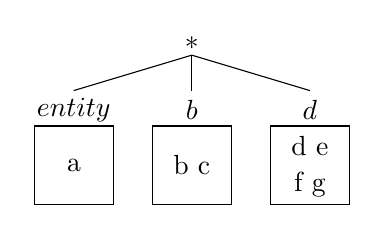
\begin{tikzpicture}
% field entity
\node at (-1,1.2) {$entity$};
\node at (-1,.5) {a};
\draw (-1.5,0) rectangle (-.5,1);
% field b
\node at (.5,1.2) {$b$};
\node at (.5,.5) {b c};
\draw (0,0) rectangle (1,1);
% field d
\node at (2,1.2) {$d$};
\node at (2,.75) {d e};
\node at (2,.25) {f g};
\draw (1.5,0) rectangle (2.5,1);
% Aggregate contributions of each field
\node at (.5,2) {*};
\draw (.5,1.9) -- (-1,1.45);
\draw (.5,1.9) -- (.5,1.45);
\draw (.5,1.9) -- (2,1.45);
\end{tikzpicture}
  		\caption{Field-based ranking model for the entity. The $*$ symbolises the aggregation of the contribution of each child node, here a field.}
		\label{fig:field-model}
  	\end{subfigure}
  	\quad
  	\begin{subfigure}{0.3\textwidth}
  		\centering
  		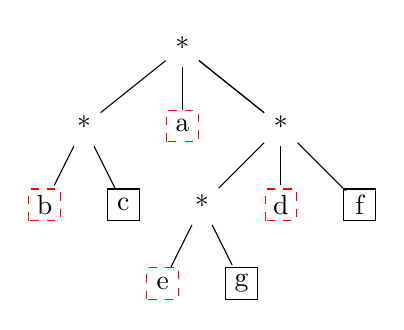
\begin{tikzpicture}
\node (a) at (-.25,0) {*};
\node (labela) at (-.25,-1) {a};
\node (b) at (-1.5,-1) {*};
\node (labelb) at (-2,-2) {b};
\node (c) at (-1,-2) {c};
\node (d) at (1,-1) {*};
\node (labeld) at (1,-2) {d};
\node (e) at (0,-2) {*};
\node (labele) at (-.5,-3) {e};
\node (f) at (2,-2) {f};
\node (g) at (.5,-3) {g};

\draw (a) -- (labela);
\draw (a) -- (b) -- (c);
\draw (b) -- (labelb);
\draw (d) -- (labeld);
\draw (e) -- (labele);
\draw (a) -- (d) -- (e) -- (g);
\draw (a) -- (d) -- (f);

\draw [red, dashed] (-2.2,-2.2) rectangle (-1.8,-1.8);
\draw (-1.2,-2.2) rectangle (-.8,-1.8);
\draw [red, dashed] (-.45,-1.2) rectangle (-.05,-.8);
\draw [red, dashed] (.8,-2.2) rectangle (1.2,-1.8);
\draw (1.8,-2.2) rectangle (2.2,-1.8);
\draw [red, dashed] (-.7,-3.2) rectangle (-.3,-2.8);
\draw (.3,-3.2) rectangle (.7,-2.8);
\end{tikzpicture}
  		\caption{The MF ranking model for the entity. A square symbolizes where the contribution of a query term is performed. Red dashed squares represents internal nodes in the entity tree that were transformed into a leaf.}
		\label{fig:mf-model}
  	\end{subfigure}
  	\quad
  	\begin{subfigure}{\textwidth}
  		\centering
	  	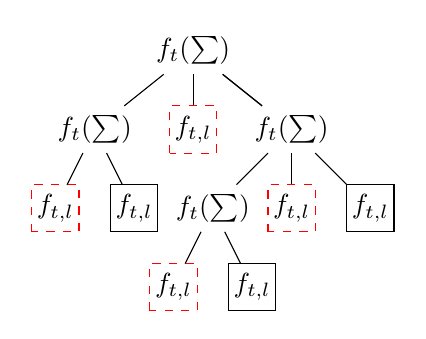
\begin{tikzpicture}
\node (a) at (-.25,0) {$f_{t}(\sum)$};
\node (labela) at (-.25,-1) {$f_{t,l}$};
\node (b) at (-1.5,-1) {$f_{t}(\sum)$};
\node (labelb) at (-2,-2) {$f_{t,l}$};
\node (c) at (-1,-2) {$f_{t,l}$};
\node (d) at (1,-1) {$f_{t}(\sum)$};
\node (labeld) at (1,-2) {$f_{t,l}$};
\node (e) at (0,-2) {$f_{t}(\sum)$};
\node (labele) at (-.5,-3) {$f_{t,l}$};
\node (f) at (2,-2) {$f_{t,l}$};
\node (g) at (.5,-3) {$f_{t,l}$};

\draw (a) -- (labela);
\draw (a) -- (b) -- (c);
\draw (b) -- (labelb);
\draw (d) -- (labeld);
\draw (e) -- (labele);
\draw (a) -- (d) -- (e) -- (g);
\draw (a) -- (d) -- (f);

\draw [red, dashed] (-2.3,-2.3) rectangle (-1.7,-1.7);
\draw (-1.3,-2.3) rectangle (-.7,-1.7);
\draw [red, dashed] (-.55,-1.3) rectangle (.05,-.7);
\draw [red, dashed] (.7,-2.3) rectangle (1.3,-1.7);
\draw (1.7,-2.3) rectangle (2.3,-1.7);
\draw [red, dashed] (-.8,-3.3) rectangle (-.2,-2.7);
\draw (.2,-3.3) rectangle (.8,-2.7);
\end{tikzpicture}
  		\caption{Normalized term frequency computation in the MF ranking for the entity.}
  		\label{fig:mf-ranking}
  	\end{subfigure}
	\caption{Abstract models for ranking a tree.}
	\label{fig:tree}
\end{figure}

\subsection{Eliteness}

In \cite{harter:1974:thesis}, Harter introduced the notion of \emph{eliteness} in order to model content-bearing terms: a document is said to be \emph{elite} in term $t$ if it is somehow ``about'' the topic associated with $t$. In \cite{robertson:1981:PMI}, Robertson et al. introduce the relationship between the eliteness of a term in a document and its frequency: an elite term is most likely to be reused in the document, hence the term frequency is used as evidence of the term eliteness in the document. In \cite{zaragoza:2004:microsoft}, Zaragoza et al. extend the notion of eliteness to documents with multiple fields. In \cite{robertson:2004:cikm}, the authors argue that the normalized frequencies of a term in each field should be combined before applying the term weighting model. Similarly in our MF model, the term eliteness in an entity is shared between its attributes. The values related to a same attribute are associated to a same topic, described by the attribute label. Therefore, a term eliteness in an attribute is shared between its values.

Although values are related to a same attribute, the relevancy of each value with regard to the query is different. We can assume that, given a same attribute, an entity where two terms occur in a single value is more relevant than another entity where each term occurs in two values. This can be seen as a way to integrate some kind of term proximity measure in the retrieval model, i.e., two words are considered close to each other when they occur in the same value. Reflecting this difference into the importance of a term using an appropriate value-specific weight can improve the ranking efficiency.

\section{MF Ranking Functions}
\label{sec:mf-function}

In this section, we describe \emph{BM25MF} and \emph{PL2MF}, the MF extensions of BM25F~\cite{zaragoza:2004:microsoft} and PL2F~\cite{macdonald:2005:clef}, respectively.
We present first the features needed for the MF ranking model and then define both extensions.

\paragraph{Ranking features.}

The MF ranking model requires the following features:
\begin{labeling}{\textbf{average attribute cardinality:}}
  \item[\textbf{leaf length:}] refers to the number of terms in the label of a leaf;
  \item[\textbf{average leaf length:}] is the mean of the siblings \emph{leaf length};
  \item[\textbf{attribute cardinality:}] is equal to the number of values an attribute possesses;
  \item[\textbf{average attribute cardinality;}] is equal to the mean of the \emph{attribute cardinality} across the entities where that attribute appears.
\end{labeling}

\subsection{BM25MF}

BM25F is extended by adapting the Equation (\ref{eq:bm25f_1}). The resulting normalised term frequency is then passed to the term frequency normalisation function in the Equation (\ref{eq:bm25f_2}).
The computation of the entity score with BM25MF consists of applying two functions, $f_{t,l}$ and $f_t$, applied on a leaf and on an internal node, respectively. After applying $f_{t,l}$ on the leaves, the results are summed up on the parent node. Then, this parent node applies the function $f_t$ on the result of the sum. This process is repeated until the root of the tree is reached.
\begin{align}
\label{bm25mf_v}
f_{t,l} & = & \frac{\alpha_v\times f_{t,e,v}}{1+b_v\times\left(\frac{l_{e,v}}{l_a}-1\right)}\\
\label{bm25mf_a}
f_{t} & = & \frac{\alpha_a\times f_{t,c}}{1+b_a\times\left(\frac{\left|{a}\right|_e}{\left|{a}\right|}-1\right)}
\end{align}
in which the following notations are used:
\begin{itemize}
\item $f_{t,e,v}$ is the frequency of the term $t$ within the value $v$ in the entity $e$;
\item $l_{e,v}$ is the \emph{value length} of the value $v$ in the entity $e$;
\item $\left|{a}\right|_e$ is the \emph{attribute cardinality} of the attribute $a$ in the entity $e$;
\item $\left|{a}\right|$ is the \emph{average attribute cardinality} of the attribute $a$;
\item $\alpha_v$ and $\alpha_a$ are respectively value and attribute specific weights; and
\item $b_a$ and $b_v$ are parameters of the term frequency's normalization, where $b_v$ is value-specific and $b_a$ attribute-specific with $(b_a,b_v)\in\left[0,1\right]^2$.
\end{itemize}

\subsection{PL2MF}

PL2F is extended by adapting the Equation (\ref{eq:pl2f}). The resulting normalised term frequency is then passed to the term frequency normalization function (\ref{eq:dfr-prisk}).
The computation of the entity score with PL2MF consists of applying two functions, $f_{t,l}$ and $f_t$, applied on a leaf and on an internal node, respectively. After applying $f_{t,l}$ on the leaves, the results are summed up on the parent node. Then, this parent node applies the function $f_t$ on the result of the sum. This process is repeated until the root of the tree is reached.
\begin{eqnarray}
  \label{eq:pl2mf_v}
  tfn_a & = & \sum_{v\in a}{\alpha_v\times f_{t,e,v} \times log_2\left(1+c_v\times\frac{l_a}{l_{e,v}}\right)}\\
  \label{eq:pl2mf_a}
  tfn & = & \sum_{a\in e}{\alpha_a\times tfn_a \times log_2\left(1+c_a\times\frac{\left|{a}\right|}{\left|{a}\right|_e}\right)}
\end{eqnarray}
where $c_a$ and $c_v$ are hyperparameters, with $c_a$ specific to the attribute $a$ and $c_v$ to the value $v$, with $(c_a,c_v) \in\; ]0,+\infty[^2$.

\minisec{Generalisation}

In Equations (\ref{bm25mf_v}) and (\ref{eq:pl2mf_v}), we normalize the term frequency based on the \emph{average attribute length} $l_a$. In Equations (\ref{bm25mf_a}) and (\ref{eq:pl2mf_a}), we further normalize the term frequency based on the \emph{average attribute cardinality} $\left|{a}\right|$.
In addition to attribute-specific weights $\alpha_a$, the MF ranking model allows value-specific weights in its implementations with the parameter $\alpha_v$. We will present value and attribute specific weights in the next section.

If we assume a single value per attribute to match field-based ranking models, then the Equations (\ref{bm25mf_v}) and (\ref{bm25mf_a}) are transformed into the Equation (\ref{eq:bm25f_2}), with $\alpha_a\times\alpha_v$ as the BM25F's attribute weight, and $b_v$ as the attribute normalization parameter. BM25MF is under this condition equivalent to BM25F. Under the same assumption, the Equations (\ref{eq:pl2mf_v}) and (\ref{eq:pl2mf_a}) are transformed into the Equation (\ref{eq:pl2f}), with $\alpha_a\times\alpha_v\times log_2(1+c_a)$ as the PL2F's attribute weight. PL2MF is under this condition equivalent to PL2F. Therefore, the MF model is a generalisation of field-based models for semi-structured data with multi-valued attributes.


\section{Weights}
\label{sec:weights}

In this section, we introduce several weights for the MF model. We first present two query-dependent weights: 
\begin{inparaenum}[(1)]
  \item the \emph{Query Coverage} weight which indicates how well the query terms are covered by an entity, an attribute or a value; and
  \item the \emph{Value Coverage} weight which indicates how well a value node is covered by a query.
\end{inparaenum}
Next, we describe the \emph{Attribute} and \emph{Entity Labels} query-independent weights.

\subsection{The Query Coverage Weight}
\label{sec:kw-factor}

The purpose of the Query Coverage (QC) weight is to lower the importance given to an entity, an attribute or a value with respect to the number of query terms it covers. This weight is combined with the ranking function using the parameters $\alpha_e$, $\alpha_a$ and $\alpha_v$. For example, given a query composed of three terms, if a value contains only occurrences of one query term, this value will then weight less than a value containing occurrences of more than one query term.

This weight integrates the IDF weight of query terms so that the coverage takes into account the importance of the terms it covers. For example, if two entities have occurrences of one of the three query terms, the coverage would then be $\frac{1}{3}$ for both. Thanks to the IDF weights, the entity with the more important term will have a higher coverage weight than the other one.

The query coverage weight is computed as:
$$
QC = \frac{\sum_{t\in X \cap q}{\omega_t^2}}{\sum_{t\in q}{\omega_t^2}}
$$
where $X$ is either a value, an attribute set or the entity and $q$ is the query.

\subsection{The Leaf Coverage Weight}
\label{sec:coverage}

The Leaf Coverage (VC) weight reflects the proportion of terms in a value matching the query, i.e., how much it is covered by the query. We assume that the more query terms match a large portion of the node, the more this node is a ``precise'' description of the query. This weight is integrated into the MF ranking function using the parameter $\alpha_v$.

The value coverage is defined as the quotient of the query terms frequencies in the value over the \emph{value length}: %
$$
c' = \frac{\sum_{t\in v \cap q}{f_{t,e,v}}}{l_V}
$$

We remark that this definition disadvantages longer values over shorter ones: given a query with two terms, a small value with occurrences of one term would receive a higher weight than a larger value with the two terms occurring, because of the \emph{value length} division.

In order to have a better control over the effect of VC, we developed the function $c_\alpha(c')$ which
\begin{inparaenum}[(1)]
  \item imposes a fixed lower bound to prevent short values receiving a higher weight than long ones; and
  \item increases as a power function to ensure a high coverage weight only when $c'$ is close to 1.
\end{inparaenum}
\begin{equation}
\label{eq:vc-norm}
c_\alpha(c') = \frac{\alpha}{1+(\alpha-1)\times c'^B}
\end{equation}
where $\alpha \in \; ]0,1[$ is a parameter that sets the lower bound of VC, and $B$ is a parameter that controls the effect of the coverage on the value. The higher $B$ is, the higher the coverage needs to be for the value node to receive a weight higher than $\alpha$.

\subsection{The Attribute and Entity Labels Weights}
\label{sec:att-subj-w}

The Attribute and Entity Labels (AEL) weights balance the importance of an entity or an attribute depending on its label. This weight is integrated into the ranking function using $\alpha_a$.
The weight value is defined empirically. Comparing the label to a regular expression, the weight is equal to:

\begin{itemize}
    \item $2$ if the label matches ``$.\star[label\,\vert\,name\,\vert\,title\,\vert\,sameas]\$$'';
    \item $0.5$ if the label matches ``$.\star[seealso\,\vert\,wikilinks]\$$'';
    \item $0.1$ if the label matches ``\url{http://www.w3.org/1999/02/22-rdf-syntax-ns\#}\_$[0-9]+\$$''; and
    \label{it:rdf:bag}
    \item $1$ otherwise.
\end{itemize}
For instance, if an attribute label is \url{http://xmlns.com/foaf/0.1/name} then a weight of $2$ is assigned.

The regular expression (\ref{it:rdf:bag}) matches an attribute URI defining items of a collection in RDF\footnote{RDF Container: \url{http://www.w3.org/TR/rdf-schema/\#ch\_container}}. It is assigned a low weight of $0.1$ to reduce the importance of terms occurring in each item of the collection. The entity label is treated as an additional attribute of the entity and is assigned a weight of $2$.


\section{Experiments}
\label{sec:experiments}

In order to evaluate the MF model, we perform several experiments using three different datasets. We start by experimenting on the normalisation parameters in order to study their impact on the effectiveness of the approach. We then compare the MF ranking functions against other traditional ones. We finally discuss the consequence of \textbf{not} considering the attribute label as a source of potential relevant terms and demonstrate the effectiveness of the proposed weights.

While there are other ways to perform entity ranking on the Web of Data, e.g., one can look at the other SemSearch 2011 candidates, in this evaluation we concentrate on demonstrating how the MF model specifically extends and improves the very popular PRF and DFR frameworks.
%\footnote{SemSearch2011: \url{http://km.aifb.kit.edu/ws/semsearch11}}

\subsection{Datasets}
\label{sec:datasets}

The datasets we are using in our experiments are the following:
\begin{description}
  \item[INEX09] a dataset of 2,491,134 triples from DBpedia containing the description of entities in English, and converted for the INEX evaluation framework~\cite{Perez-Aguera:2010:UBS};
  \item[SS10] the ``Billion Triple Challenge''\footnote{Billion Triple Challenge: \url{http://vmlion25.deri.ie}} (BTC) dataset, containing more than one billion triples, with the assessments (a file containing relevance judgments on a sample of query answers) of the SemSearch2010\footnote{SemSearch2010: \url{http://km.aifb.kit.edu/ws/semsearch10}} challenge;
  \item[SS11] the BTC dataset with the assessments of the ``Entity Search track'' of the SemSearch2011\footnote{SemSearch2011: \url{http://km.aifb.kit.edu/ws/semsearch11/}} challenge.
\end{description}
The INEX09 dataset is significantly different than the other two based on BTC. Indeed, BTC is a heterogeneous dataset, created from web crawls of several search engines. INEX09 is a highly curated dataset from DBpedia.

%\subsection{Effectiveness of the MF Ranking Model}
%\label{sec:mv-fields-effectiveness}
%
% Next we perform a comparison between the MF extensions, i.e., BM25MF and PL2MF, against other ranking approaches.

\subsection{\emph{The Normalisation Parameters}}
\label{sec:norm-exp}

In this section, we study the impact on the ranking of the normalisation parameters. In addition to the length normalisation of field-based ranking function (Normalisation~\ref{norm:content}), the MF ranking model offers an additional normalisation on the attribute's cardinality (Normalisation~\ref{norm:degree}). The effectiveness of the PRF and DFR frameworks depends on finding the right values for the normalisation parameters. However, these parameters are highly dependent on the dataset.\\

Figures~\ref{fig:bm25mf-norm} and~\ref{fig:pl2mf-norm} depict the impact of the normalisation parameters on the ranking performance of BM25MF and PL2MF, respectively. For all three datasets, the figures depict on the \textbf{Y} axis the Mean Average Precision (MAP) scores, and on the \textbf{X} axis the Normalisation~\ref{norm:content}, i.e., with parameter $b_v$ in Figure~\ref{fig:bm25mf-norm} (resp., parameter $c_v$ in Figure~\ref{fig:pl2mf-norm}). Each curve plots the results with a fixed Normalisation~\ref{norm:degree} parameter, i.e., $b_a$ in Figure~\ref{fig:bm25mf-norm} and $c_a$ in Figure~\ref{fig:pl2mf-norm}.

The grid of parameters values in Figure~\ref{fig:bm25mf-norm} ranges from $0$ to $1$ with a step of $0.1$. In Figure~\ref{fig:pl2mf-norm}, the grid ranges from $0.5$ to $10.5$ with a step of $1$. Although these parameters can be attribute and value-specific, this experiment considers a constant parameter in order to reduce the number of combinations and to lower the variability of the results. Dashed lines depict the MAP scores of BM25F and PL2F and solid lines the scores of their MF extension, BM25MF and PL2MF respectively.\\

These plots show that Normalisation~\ref{norm:degree}, the normalisation introduced with the MF ranking model, improves the performance. Indeed, the Normalisation~\ref{norm:content} parameters $b_v$ and $c_v$, which are traditional to the field-based ranking model, do not grasp completely the heterogeneity in the data, which results in lower performance when compared to the MF extensions. This indicates that the distinction between leaves within an attribute has a positive effect on the ranking.

\begin{figure}
	\centering
	\begin{subfigure}{\textwidth}
		\centering
		\begin{subfigure}[b]{.3\textwidth}
	\renewcommand\thesubfigure{\alph{subfigure}1}
	\centering
	\resizebox{\textwidth}{!}{
	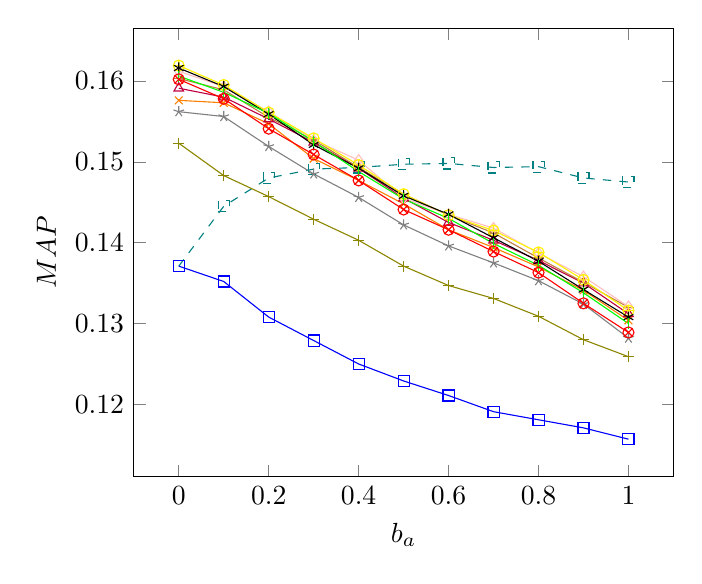
\begin{tikzpicture}
	\begin{axis}[
	xlabel=$b_a$,
	ylabel=$MAP$,
	% y label style={rotate=-90}
	]

%%%%%%%%%%%
%% x = b_v, y = b_a
%%%%%%%%%%%
%\addplot[mark=square, style=solid, color=blue] coordinates
%{ (0.0,  0.1371 ) (0.1,  0.1523 ) (0.2,  0.1562 ) (0.3,  0.1576 ) (0.4,  0.1591 ) (0.5,  0.1603 ) (0.6,  0.1612 ) (0.7,  0.1619 ) (0.8,  0.1616 ) (0.9,  0.1606 ) (1.0,  0.1602 ) };

%\addplot[mark=+, style=solid, color=olive] coordinates
%{ (0.0,  0.1352 ) (0.1,  0.1483 ) (0.2,  0.1556 ) (0.3,  0.1573 ) (0.4,  0.158 ) (0.5,  0.1589 ) (0.6,  0.1593 ) (0.7,  0.1595 ) (0.8,  0.1593 ) (0.9,  0.1586 ) (1.0,  0.1578 ) };

%\addplot[mark=star, style=solid, color=gray] coordinates
%{ (0.0,  0.1308 ) (0.1,  0.1457 ) (0.2,  0.1519 ) (0.3,  0.1547 ) (0.4,  0.1553 ) (0.5,  0.1555 ) (0.6,  0.1562 ) (0.7,  0.1561 ) (0.8,  0.1559 ) (0.9,  0.156 ) (1.0,  0.1541 ) };

%\addplot[mark=x, style=solid, color=orange] coordinates
%{ (0.0,  0.1279 ) (0.1,  0.1429 ) (0.2,  0.1485 ) (0.3,  0.1504 ) (0.4,  0.1524 ) (0.5,  0.1527 ) (0.6,  0.1527 ) (0.7,  0.1529 ) (0.8,  0.1521 ) (0.9,  0.1525 ) (1.0,  0.1509 ) };

%\addplot[mark=triangle, style=solid, color=purple] coordinates
%{ (0.0,  0.125 ) (0.1,  0.1403 ) (0.2,  0.1456 ) (0.3,  0.1477 ) (0.4,  0.1492 ) (0.5,  0.1493 ) (0.6,  0.1502 ) (0.7,  0.1496 ) (0.8,  0.1492 ) (0.9,  0.1488 ) (1.0,  0.1477 ) };

%\addplot[mark=-, style=solid, color=brown] coordinates
%{ (0.0,  0.1229 ) (0.1,  0.1371 ) (0.2,  0.1422 ) (0.3,  0.1448 ) (0.4,  0.1455 ) (0.5,  0.146 ) (0.6,  0.1455 ) (0.7,  0.146 ) (0.8,  0.1458 ) (0.9,  0.1454 ) (1.0,  0.1441 ) };

%\addplot[mark=diamond, style=solid, color=pink] coordinates
%{ (0.0,  0.1211 ) (0.1,  0.1347 ) (0.2,  0.1396 ) (0.3,  0.1416 ) (0.4,  0.1425 ) (0.5,  0.1434 ) (0.6,  0.1435 ) (0.7,  0.1434 ) (0.8,  0.1435 ) (0.9,  0.143 ) (1.0,  0.1416 ) };

%\addplot[mark=oplus, style=solid, color=yellow] coordinates
%{ (0.0,  0.1191 ) (0.1,  0.1331 ) (0.2,  0.1375 ) (0.3,  0.1394 ) (0.4,  0.1403 ) (0.5,  0.1412 ) (0.6,  0.1418 ) (0.7,  0.1415 ) (0.8,  0.1406 ) (0.9,  0.1399 ) (1.0,  0.1389 ) };

%\addplot[mark=asterisk, style=solid, color=black] coordinates
%{ (0.0,  0.1181 ) (0.1,  0.1309 ) (0.2,  0.1353 ) (0.3,  0.137 ) (0.4,  0.1378 ) (0.5,  0.1381 ) (0.6,  0.1387 ) (0.7,  0.1388 ) (0.8,  0.1377 ) (0.9,  0.1372 ) (1.0,  0.1363 ) };

%\addplot[mark=|, style=solid, color=green] coordinates
%{ (0.0,  0.1171 ) (0.1,  0.128 ) (0.2,  0.1324 ) (0.3,  0.1341 ) (0.4,  0.135 ) (0.5,  0.1351 ) (0.6,  0.1358 ) (0.7,  0.1354 ) (0.8,  0.1342 ) (0.9,  0.1338 ) (1.0,  0.1325 ) };

%\addplot[mark=otimes, style=solid, color=red] coordinates
%{ (0.0,  0.1157 ) (0.1,  0.1259 ) (0.2,  0.1282 ) (0.3,  0.1304 ) (0.4,  0.1312 ) (0.5,  0.132 ) (0.6,  0.1321 ) (0.7,  0.1316 ) (0.8,  0.1308 ) (0.9,  0.13 ) (1.0,  0.1289 ) };

%%%%%%%%%%%
%% x = b_v, y = b_a
%%%%%%%%%%%
\addplot[mark=square, style=dashed, color=teal] coordinates
{ (0, 0.1371) (.1, 0.1445) (.2, 0.148) (.3, 0.1491) (.4, 0.1493) (.5, 0.1497) (.6, 0.1498) (.7, 0.1493) (.8, 0.1494) (.9, 0.148) (1.0, 0.1475) };

\addplot[mark=square, style=solid, color=blue] coordinates
{ (0.0, 0.1371) (0.1, 0.1352) (0.2, 0.1308) (0.3, 0.1279) (0.4, 0.125) (0.5, 0.1229) (0.6, 0.1211) (0.7, 0.1191) (0.8, 0.1181) (0.9, 0.1171) (1.0, 0.1157) };

\addplot[mark=+, style=solid, color=olive] coordinates
{ (0.0, 0.1523) (0.1, 0.1483) (0.2, 0.1457) (0.3, 0.1429) (0.4, 0.1403) (0.5, 0.1371) (0.6, 0.1347) (0.7, 0.1331) (0.8, 0.1309) (0.9, 0.128) (1.0, 0.1259) };

\addplot[mark=star, style=solid, color=gray] coordinates
{ (0.0, 0.1562) (0.1, 0.1556) (0.2, 0.1519) (0.3, 0.1485) (0.4, 0.1456) (0.5, 0.1422) (0.6, 0.1396) (0.7, 0.1375) (0.8, 0.1353) (0.9, 0.1324) (1.0, 0.1282) };

\addplot[mark=x, style=solid, color=orange] coordinates
{ (0.0, 0.1576) (0.1, 0.1573) (0.2, 0.1547) (0.3, 0.1504) (0.4, 0.1477) (0.5, 0.1448) (0.6, 0.1416) (0.7, 0.1394) (0.8, 0.137) (0.9, 0.1341) (1.0, 0.1304) };

\addplot[mark=triangle, style=solid, color=purple] coordinates
{ (0.0, 0.1591) (0.1, 0.158) (0.2, 0.1553) (0.3, 0.1524) (0.4, 0.1492) (0.5, 0.1455) (0.6, 0.1425) (0.7, 0.1403) (0.8, 0.1378) (0.9, 0.135) (1.0, 0.1312) };

\addplot[mark=-, style=solid, color=brown] coordinates
{ (0.0, 0.1603) (0.1, 0.1589) (0.2, 0.1555) (0.3, 0.1527) (0.4, 0.1493) (0.5, 0.146) (0.6, 0.1434) (0.7, 0.1412) (0.8, 0.1381) (0.9, 0.1351) (1.0, 0.132) };

\addplot[mark=diamond, style=solid, color=pink] coordinates
{ (0.0, 0.1612) (0.1, 0.1593) (0.2, 0.1562) (0.3, 0.1527) (0.4, 0.1502) (0.5, 0.1455) (0.6, 0.1435) (0.7, 0.1418) (0.8, 0.1387) (0.9, 0.1358) (1.0, 0.1321) };

\addplot[mark=oplus, style=solid, color=yellow] coordinates
{ (0.0, 0.1619) (0.1, 0.1595) (0.2, 0.1561) (0.3, 0.1529) (0.4, 0.1496) (0.5, 0.146) (0.6, 0.1434) (0.7, 0.1415) (0.8, 0.1388) (0.9, 0.1354) (1.0, 0.1316) };

\addplot[mark=asterisk, style=solid, color=black] coordinates
{ (0.0, 0.1616) (0.1, 0.1593) (0.2, 0.1559) (0.3, 0.1521) (0.4, 0.1492) (0.5, 0.1458) (0.6, 0.1435) (0.7, 0.1406) (0.8, 0.1377) (0.9, 0.1342) (1.0, 0.1308) };

\addplot[mark=|, style=solid, color=green] coordinates
{ (0.0, 0.1606) (0.1, 0.1586) (0.2, 0.156) (0.3, 0.1525) (0.4, 0.1488) (0.5, 0.1454) (0.6, 0.143) (0.7, 0.1399) (0.8, 0.1372) (0.9, 0.1338) (1.0, 0.13) };

\addplot[mark=otimes, style=solid, color=red] coordinates
{ (0.0, 0.1602) (0.1, 0.1578) (0.2, 0.1541) (0.3, 0.1509) (0.4, 0.1477) (0.5, 0.1441) (0.6, 0.1416) (0.7, 0.1389) (0.8, 0.1363) (0.9, 0.1325) (1.0, 0.1289) };

\end{axis}
\end{tikzpicture}}

	\caption{INEX09}
\end{subfigure}
\quad%
\begin{subfigure}[b]{.3\textwidth}
	\addtocounter{subfigure}{-1}
	\renewcommand\thesubfigure{\alph{subfigure}2}
	\centering
	\resizebox{\textwidth}{!}{
	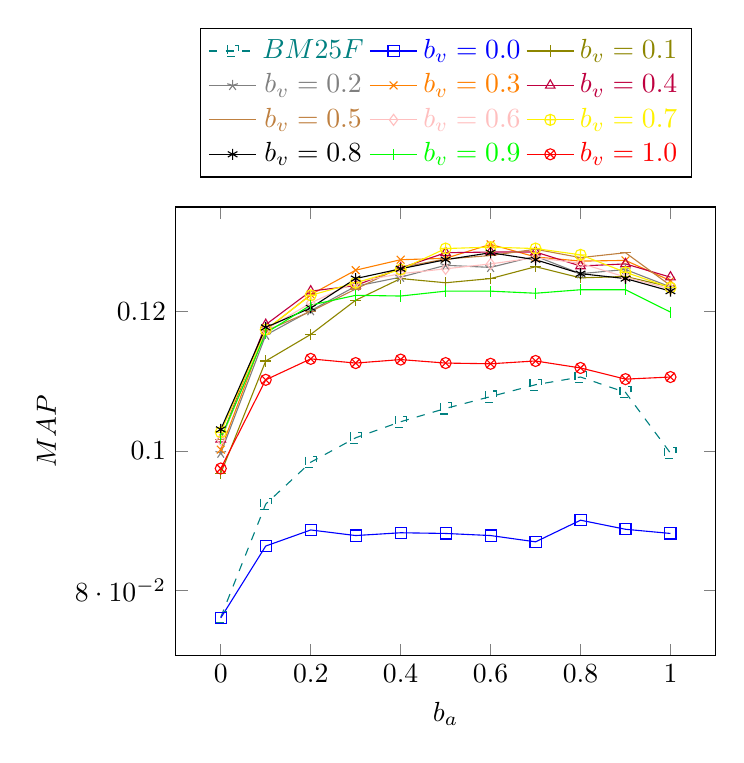
\begin{tikzpicture}
	\begin{axis}[
	  legend entries={
	    [teal]$BM25F$,
		[blue]$b_v = 0.0$,
	 	[olive]$b_v = 0.1$,
	  	[gray]$b_v = 0.2$,
	  	[orange]$b_v = 0.3$,
		[purple]$b_v = 0.4$,
	 	[brown]$b_v = 0.5$,
	  	[pink]$b_v = 0.6$,
	  	[yellow]$b_v = 0.7$,
		[black]$b_v = 0.8$,
	 	[green]$b_v = 0.9$,
	 	[red]$b_v = 1.0$
	  },
	  legend columns=3,
      legend style={at={(0.5,1.4)},anchor=north},
	  xlabel=$b_a$,
	  ylabel=$MAP$,
	  % y label style={rotate=-90},
	]

%%%%%%%%%%%
%% x = c_v, y = c_a
%%%%%%%%%%%
%\addplot[mark=square, style=solid, color=blue] coordinates
%{ (0.0, 0.0761) (0.1, 0.0968) (0.2, 0.0997) (0.3, 0.1002) (0.4, 0.1017) (0.5, 0.1016) (0.6, 0.1016) (0.7, 0.1027) (0.8, 0.1031) (0.9, 0.1018) (1.0, 0.0975) };

%\addplot[mark=+, style=solid, color=olive] coordinates
%{ (0.0, 0.0864) (0.1, 0.1129) (0.2, 0.1166) (0.3, 0.1173) (0.4, 0.1181) (0.5, 0.1172) (0.6, 0.1174) (0.7, 0.1174) (0.8, 0.1177) (0.9, 0.1169) (1.0, 0.1102) };

%\addplot[mark=star, style=solid, color=gray] coordinates
%{ (0.0, 0.0887) (0.1, 0.1167) (0.2, 0.1201) (0.3, 0.1224) (0.4, 0.1229) (0.5, 0.12) (0.6, 0.1212) (0.7, 0.1223) (0.8, 0.1205) (0.9, 0.1209) (1.0, 0.1132) };

%\addplot[mark=x, style=solid, color=orange] coordinates
%{ (0.0, 0.0879) (0.1, 0.1216) (0.2, 0.1236) (0.3, 0.1259) (0.4, 0.1237) (0.5, 0.1232) (0.6, 0.1242) (0.7, 0.1241) (0.8, 0.1247) (0.9, 0.1223) (1.0, 0.1126) };

%\addplot[mark=triangle, style=solid, color=purple] coordinates
%{ (0.0, 0.0883) (0.1, 0.1247) (0.2, 0.1249) (0.3, 0.1274) (0.4, 0.1262) (0.5, 0.1263) (0.6, 0.1254) (0.7, 0.126) (0.8, 0.1261) (0.9, 0.1222) (1.0, 0.1131) };

%\addplot[mark=-, style=solid, color=brown] coordinates
%{ (0.0, 0.0882) (0.1, 0.1241) (0.2, 0.1266) (0.3, 0.1276) (0.4, 0.1284) (0.5, 0.1275) (0.6, 0.1261) (0.7, 0.129) (0.8, 0.1274) (0.9, 0.1229) (1.0, 0.1126) };

%\addplot[mark=diamond, style=solid, color=pink] coordinates
%{ (0.0, 0.0879) (0.1, 0.1247) (0.2, 0.1263) (0.3, 0.1296) (0.4, 0.1285) (0.5, 0.128) (0.6, 0.1268) (0.7, 0.1292) (0.8, 0.1284) (0.9, 0.1229) (1.0, 0.1125) };

%\addplot[mark=oplus, style=solid, color=yellow] coordinates
%{ (0.0, 0.087) (0.1, 0.1264) (0.2, 0.1279) (0.3, 0.1278) (0.4, 0.1285) (0.5, 0.1289) (0.6, 0.1277) (0.7, 0.129) (0.8, 0.1274) (0.9, 0.1226) (1.0, 0.1129) };

%\addplot[mark=asterisk, style=solid, color=black] coordinates
%{ (0.0, 0.0901) (0.1, 0.1248) (0.2, 0.1254) (0.3, 0.1272) (0.4, 0.1265) (0.5, 0.1277) (0.6, 0.1269) (0.7, 0.1281) (0.8, 0.1254) (0.9, 0.1231) (1.0, 0.1119) };

%\addplot[mark=|, style=solid, color=green] coordinates
%{ (0.0, 0.0888) (0.1, 0.125) (0.2, 0.126) (0.3, 0.1273) (0.4, 0.1268) (0.5, 0.1284) (0.6, 0.1249) (0.7, 0.1256) (0.8, 0.1247) (0.9, 0.1231) (1.0, 0.1103) };

%\addplot[mark=otimes, style=solid, color=red] coordinates
%{ (0.0, 0.0882) (0.1, 0.1235) (0.2, 0.1235) (0.3, 0.1244) (0.4, 0.1249) (0.5, 0.1237) (0.6, 0.1232) (0.7, 0.1234) (0.8, 0.1229) (0.9, 0.1199) (1.0, 0.1106) };

%%%%%%%%%%%
%% x = b_a, y = b_v
%%%%%%%%%%%
\addplot[mark=square, style=dashed, color=teal] coordinates
{ (0, 0.0762) (.1, 0.0924) (.2, 0.0984) (.3, 0.1019) (.4, 0.1042) (.5, 0.1061) (.6, 0.1078) (.7, 0.1095) (.8, 0.1106) (.9, 0.1084) (1.0, 0.0997) };

\addplot[mark=square, style=solid, color=blue] coordinates
{ (0.0, 0.0761) (0.1, 0.0864) (0.2, 0.0887) (0.3, 0.0879) (0.4, 0.0883) (0.5, 0.0882) (0.6, 0.0879) (0.7, 0.087) (0.8, 0.0901) (0.9, 0.0888) (1.0, 0.0882) };

\addplot[mark=+, style=solid, color=olive] coordinates
{ (0.0, 0.0968) (0.1, 0.1129) (0.2, 0.1167) (0.3, 0.1216) (0.4, 0.1247) (0.5, 0.1241) (0.6, 0.1247) (0.7, 0.1264) (0.8, 0.1248) (0.9, 0.125) (1.0, 0.1235) };

\addplot[mark=star, style=solid, color=gray] coordinates
{ (0.0, 0.0997) (0.1, 0.1166) (0.2, 0.1201) (0.3, 0.1236) (0.4, 0.1249) (0.5, 0.1266) (0.6, 0.1263) (0.7, 0.1279) (0.8, 0.1254) (0.9, 0.126) (1.0, 0.1235) };

\addplot[mark=x, style=solid, color=orange] coordinates
{ (0.0, 0.1002) (0.1, 0.1173) (0.2, 0.1224) (0.3, 0.1259) (0.4, 0.1274) (0.5, 0.1276) (0.6, 0.1296) (0.7, 0.1278) (0.8, 0.1272) (0.9, 0.1273) (1.0, 0.1244) };

\addplot[mark=triangle, style=solid, color=purple] coordinates
{ (0.0, 0.1017) (0.1, 0.1181) (0.2, 0.1229) (0.3, 0.1237) (0.4, 0.1262) (0.5, 0.1284) (0.6, 0.1285) (0.7, 0.1285) (0.8, 0.1265) (0.9, 0.1268) (1.0, 0.1249) };

\addplot[mark=-, style=solid, color=brown] coordinates
{ (0.0, 0.1016) (0.1, 0.1172) (0.2, 0.12) (0.3, 0.1232) (0.4, 0.1263) (0.5, 0.1275) (0.6, 0.128) (0.7, 0.1289) (0.8, 0.1277) (0.9, 0.1284) (1.0, 0.1237) };

\addplot[mark=diamond, style=solid, color=pink] coordinates
{ (0.0, 0.1016) (0.1, 0.1174) (0.2, 0.1212) (0.3, 0.1242) (0.4, 0.1254) (0.5, 0.1261) (0.6, 0.1268) (0.7, 0.1277) (0.8, 0.1269) (0.9, 0.1249) (1.0, 0.1232) };

\addplot[mark=oplus, style=solid, color=yellow] coordinates
{ (0.0, 0.1027) (0.1, 0.1174) (0.2, 0.1223) (0.3, 0.1241) (0.4, 0.126) (0.5, 0.129) (0.6, 0.1292) (0.7, 0.129) (0.8, 0.1281) (0.9, 0.1256) (1.0, 0.1234) };

\addplot[mark=asterisk, style=solid, color=black] coordinates
{ (0.0, 0.1031) (0.1, 0.1177) (0.2, 0.1205) (0.3, 0.1247) (0.4, 0.1261) (0.5, 0.1274) (0.6, 0.1284) (0.7, 0.1274) (0.8, 0.1254) (0.9, 0.1247) (1.0, 0.1229) };

\addplot[mark=|, style=solid, color=green] coordinates
{ (0.0, 0.1018) (0.1, 0.1169) (0.2, 0.1209) (0.3, 0.1223) (0.4, 0.1222) (0.5, 0.1229) (0.6, 0.1229) (0.7, 0.1226) (0.8, 0.1231) (0.9, 0.1231) (1.0, 0.1199) };

\addplot[mark=otimes, style=solid, color=red] coordinates
{ (0.0, 0.0975) (0.1, 0.1102) (0.2, 0.1132) (0.3, 0.1126) (0.4, 0.1131) (0.5, 0.1126) (0.6, 0.1125) (0.7, 0.1129) (0.8, 0.1119) (0.9, 0.1103) (1.0, 0.1106) };

\end{axis}
\end{tikzpicture}}

	\caption{SS10}
\end{subfigure}
\quad%
\begin{subfigure}[b]{.3\textwidth}
	\addtocounter{subfigure}{-1}
	\renewcommand\thesubfigure{\alph{subfigure}3}
	\centering
	\resizebox{\textwidth}{!}{
	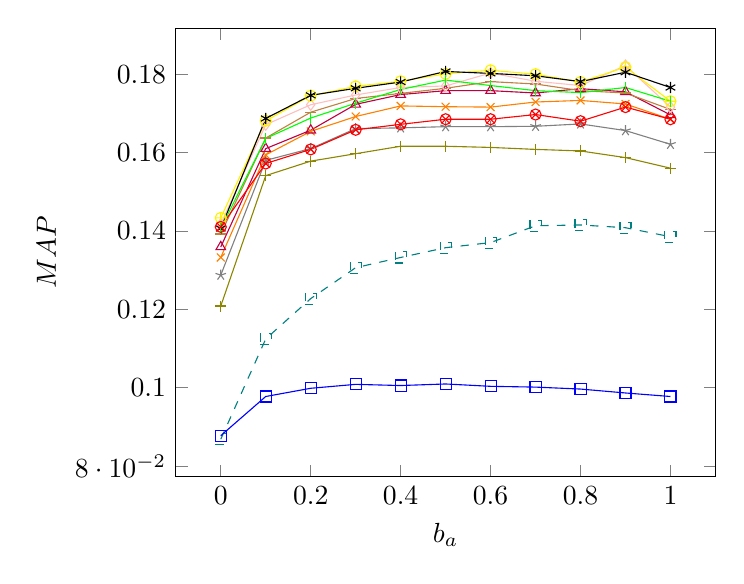
\begin{tikzpicture}
	\begin{axis}[
		xlabel=$b_a$,
		ylabel=$MAP$,
		% y label style={rotate=-90},
	]

%%%%%%%%%%%
%% x = b_v, y = b_a
%%%%%%%%%%%
%\addplot[mark=square, style=solid, color=blue] coordinates
%{ (0.0,  0.0877) (0.1,  0.1208) (0.2,  0.1287) (0.3,  0.1332) (0.4,  0.1359) (0.5,  0.1392) (0.6,  0.1417) (0.7,  0.1433) (0.8, 0.1406) (0.9, 0.1406) (1.0, 0.141) };

%\addplot[mark=+, style=solid, color=olive] coordinates
%{ (0.0,  0.0977) (0.1, 0.1541 ) (0.2,  0.158) (0.3, 0.1594) (0.4,  0.161) (0.5,  0.1637) (0.6, 0.1671) (0.7,  0.1681) (0.8, 0.1687) (0.9,  0.1636) (1.0,  0.1572) };

%\addplot[mark=star, style=solid, color=gray] coordinates
%{ (0.0, 0.0998 ) (0.1,  0.1578) (0.2,  0.161) (0.3,  0.1654) (0.4,  0.1657) (0.5, 0.1703) (0.6,  0.1722) (0.7, 0.1745) (0.8,  0.1746) (0.9,  0.1688) (1.0, 0.1608) };

%\addplot[mark=x, style=solid, color=orange] coordinates
%{ (0.0,  0.1008) (0.1,  0.1597) (0.2,  0.1661) (0.3,  0.1692) (0.4,  0.1723) (0.5, 0.1738) (0.6, 0.1747) (0.7, 0.1769) (0.8,  0.1764) (0.9,  0.1726) (1.0, 0.1658) };

%\addplot[mark=triangle, style=solid, color=purple] coordinates
%{ (0.0,  0.1005) (0.1,  0.1616) (0.2,  0.1663) (0.3,  0.1719) (0.4, 0.1748 ) (0.5, 0.1751) (0.6,0.1766 ) (0.7, 0.1782) (0.8,  0.178) (0.9,  0.1761) (1.0,  0.1672) };

%\addplot[mark=-, style=solid, color=brown] coordinates
%{ (0.0,  0.1009) (0.1,  0.1616) (0.2,  0.1666) (0.3,  0.1717) (0.4,  0.1758) (0.5, 0.1764 ) (0.6, 0.177) (0.7, 0.1801) (0.8,  0.1807) (0.9,  0.1785) (1.0, 0.1685) };

%\addplot[mark=diamond, style=solid, color=pink] coordinates
%{ (0.0,  0.1003) (0.1,  0.1613) (0.2,  0.1666) (0.3,  0.1716) (0.4,  0.1758) (0.5, 0.1781) (0.6, 0.1803) (0.7, 0.181) (0.8,  0.1802) (0.9,  0.1771) (1.0,  0.1685) };

%\addplot[mark=oplus, style=solid, color=yellow] coordinates
%{ (0.0,  0.1001) (0.1,  0.1608) (0.2,  0.1667) (0.3,  0.1729) (0.4,  0.1752) (0.5, 0.1775) (0.6, 0.1782) (0.7, 0.18) (0.8, 0.1796 ) (0.9,  0.1758) (1.0,  0.1697) };

%\addplot[mark=asterisk, style=solid, color=black] coordinates
%{ (0.0, 0.0996 ) (0.1,  0.1604) (0.2, 0.1673 ) (0.3, 0.1733 ) (0.4, 0.1763 ) (0.5, 0.1758 ) (0.6, 0.1771) (0.7, 0.178) (0.8,  0.1781) (0.9,  0.1753) (1.0,  0.168) };

%\addplot[mark=|, style=solid, color=green] coordinates
%{ (0.0,  0.0986) (0.1, 0.1587 ) (0.2, 0.1656 ) (0.3, 0.1724 ) (0.4, 0.1755 ) (0.5, 0.1752 ) (0.6, 0.1822) (0.7, 0.1818) (0.8, 0.1805 ) (0.9, 0.1766 ) (1.0, 0.1716 )
%};

%\addplot[mark=otimes, style=solid, color=red] coordinates
%{ (0.0, 0.0977 ) (0.1, 0.156 ) (0.2, 0.1621 ) (0.3, 0.1685 ) (0.4, 0.1696 ) (0.5, 0.171 ) (0.6, 0.1716 ) (0.7, 0.1731 ) (0.8, 0.1766) (0.9, 0.1731) (1.0, 0.1685 ) };

%%%%%%%%%%%
%% x = b_a, y = b_v
%%%%%%%%%%%

\addplot[mark=square, style=dashed, color=teal] coordinates
{ (0, 0.0868) (.1, 0.1124) (.2, 0.1227) (.3, 0.1306) (.4, 0.1332) (.5, 0.1357) (.6, 0.137) (.7, 0.1413) (.8, 0.1415) (.9, 0.1408) (1.0, 0.1385) };

\addplot[mark=square, style=solid, color=blue] coordinates
{ (0.0, 0.0877) (0.1, 0.0977) (0.2, 0.0998) (0.3, 0.1008) (0.4, 0.1005) (0.5, 0.1009) (0.6, 0.1003) (0.7, 0.1001) (0.8, 0.0996) (0.9, 0.0986) (1.0, 0.0977) };

\addplot[mark=+, style=solid, color=olive] coordinates
{ (0.0, 0.1208) (0.1, 0.1541) (0.2, 0.1578) (0.3, 0.1597) (0.4, 0.1616) (0.5, 0.1616) (0.6, 0.1613) (0.7, 0.1608) (0.8, 0.1604) (0.9, 0.1587) (1.0, 0.156) };

\addplot[mark=star, style=solid, color=gray] coordinates
{ (0.0, 0.1287) (0.1, 0.158) (0.2, 0.161) (0.3, 0.1661) (0.4, 0.1663) (0.5, 0.1666) (0.6, 0.1666) (0.7, 0.1667) (0.8, 0.1673) (0.9, 0.1656) (1.0, 0.1621) };

\addplot[mark=x, style=solid, color=orange] coordinates
{ (0.0, 0.1332) (0.1, 0.1594) (0.2, 0.1654) (0.3, 0.1692) (0.4, 0.1719) (0.5, 0.1717) (0.6, 0.1716) (0.7, 0.1729) (0.8, 0.1733) (0.9, 0.1724) (1.0, 0.1685) };

\addplot[mark=triangle, style=solid, color=purple] coordinates
{ (0.0, 0.1359) (0.1, 0.161) (0.2, 0.1657) (0.3, 0.1723) (0.4, 0.1748) (0.5, 0.1758) (0.6, 0.1758) (0.7, 0.1752) (0.8, 0.1763) (0.9, 0.1755) (1.0, 0.1696) };

\addplot[mark=-, style=solid, color=brown] coordinates
{ (0.0, 0.1392) (0.1, 0.1637) (0.2, 0.1703) (0.3, 0.1738) (0.4, 0.1751) (0.5, 0.1764) (0.6, 0.1781) (0.7, 0.1775) (0.8, 0.1758) (0.9, 0.1752) (1.0, 0.171) };

\addplot[mark=diamond, style=solid, color=pink] coordinates
{ (0.0, 0.1417) (0.1, 0.1671) (0.2, 0.1722) (0.3, 0.1747) (0.4, 0.1766) (0.5, 0.177) (0.6, 0.1803) (0.7, 0.1782) (0.8, 0.1771) (0.9, 0.1822) (1.0, 0.1716) };

\addplot[mark=oplus, style=solid, color=yellow] coordinates
{ (0.0, 0.1433) (0.1, 0.1681) (0.2, 0.1745) (0.3, 0.1769) (0.4, 0.1782) (0.5, 0.1801) (0.6, 0.181) (0.7, 0.18) (0.8, 0.178) (0.9, 0.1818) (1.0, 0.1731) };

\addplot[mark=asterisk, style=solid, color=black] coordinates
{ (0.0, 0.1406) (0.1, 0.1687) (0.2, 0.1746) (0.3, 0.1764) (0.4, 0.178) (0.5, 0.1807) (0.6, 0.1802) (0.7, 0.1796) (0.8, 0.1781) (0.9, 0.1805) (1.0, 0.1766) };

\addplot[mark=|, style=solid, color=green] coordinates
{ (0.0, 0.1406) (0.1, 0.1636) (0.2, 0.1688) (0.3, 0.1726) (0.4, 0.1761) (0.5, 0.1785) (0.6, 0.1771) (0.7, 0.1758) (0.8, 0.1753) (0.9, 0.1766) (1.0, 0.1731) };

\addplot[mark=otimes, style=solid, color=red] coordinates
{ (0.0, 0.141) (0.1, 0.1572) (0.2, 0.1608) (0.3, 0.1658) (0.4, 0.1672) (0.5, 0.1685) (0.6, 0.1685) (0.7, 0.1697) (0.8, 0.168) (0.9, 0.1716) (1.0, 0.1685) };

\end{axis}
\end{tikzpicture}}
\caption{SS11}
\end{subfigure}

		\addtocounter{subfigure}{-1}
		\caption{Evaluation of BM25MF normalisation parameters. A curve plots a fixed $b_v$ value (Equation~(\ref{bm25mf_v})) with $b_a$ (Equation~(\ref{bm25mf_a})) varying from $0$ to $1$ with a precision step of $0.1$.}
		\label{fig:bm25mf-norm}
	\end{subfigure}
	\qquad
	\begin{subfigure}{\textwidth}
		\centering
		\begin{subfigure}[b]{.3\textwidth}
	\renewcommand\thesubfigure{\alph{subfigure}1}
	\centering
	\resizebox{\textwidth}{!}{
	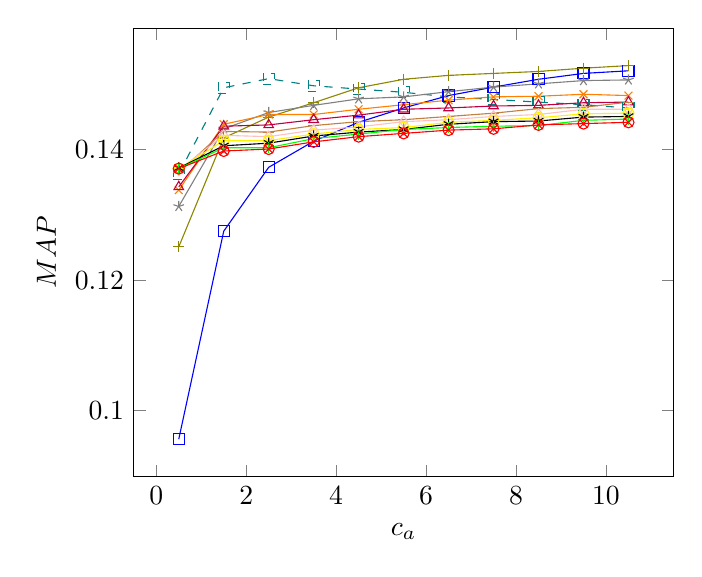
\begin{tikzpicture}
		\begin{axis}[
		xlabel=$c_a$,
		ylabel=$MAP$,
		% y label style={rotate=-90}
	]
%%%%%%%%%%%%%%%%%%%%
%%% x=cv y=ca, from 5 to 50, with step of 5
%%%%%%%%%%%%%%%%%%%%
%%\addplot[mark=square, style=solid, color=blue] coordinates

%\addplot[mark=+, style=solid, color=olive] coordinates
%{ (0, 0.1492) (5, 0.1451) (10, 0.1425) (15, 0.1411) (20, 0.1397) (25, 0.1381) (30, 0.1373) (35, 0.137) (40, 0.1365) (45, 0.136) (50, 0.1356) };

%\addplot[mark=star, style=solid, color=gray] coordinates
%{ (0, 0.1468) (5, 0.1469) (10, 0.1444) (15, 0.1421) (20, 0.1408) (25, 0.1397) (30, 0.1387) (35, 0.1381) (40, 0.1377) (45, 0.1372) (50, 0.1369) };

%\addplot[mark=x, style=solid, color=orange] coordinates
%{ (0, 0.1452) (5, 0.1476) (10, 0.1442) (15, 0.1419) (20, 0.1407) (25, 0.1397) (30, 0.1388) (35, 0.1382) (40, 0.1377) (45, 0.1373) (50, 0.1369) };

%\addplot[mark=triangle, style=solid, color=purple] coordinates
%{ (0, 0.1443) (5, 0.1475) (10, 0.1435) (15, 0.1415) (20, 0.1403) (25, 0.1393) (30, 0.1384) (35, 0.1379) (40, 0.1375) (45, 0.1371) (50, 0.1369) };

%\addplot[mark=-, style=solid, color=brown] coordinates
%{ (0, 0.1431) (5, 0.1472) (10, 0.1435) (15, 0.1413) (20, 0.1399) (25, 0.139) (30, 0.1384) (35, 0.1378) (40, 0.1374) (45, 0.1371) (50, 0.1367) };

%\addplot[mark=diamond, style=solid, color=pink] coordinates
%{ (0, 0.1422) (5, 0.1472) (10, 0.1432) (15, 0.1412) (20, 0.1401) (25, 0.1393) (30, 0.1385) (35, 0.1379) (40, 0.1376) (45, 0.1372) (50, 0.137) };

%\addplot[mark=oplus, style=solid, color=yellow] coordinates
%{ (0, 0.1418) (5, 0.1473) (10, 0.1431) (15, 0.1411) (20, 0.1401) (25, 0.1392) (30, 0.1387) (35, 0.1383) (40, 0.1378) (45, 0.1374) (50, 0.137) };

%\addplot[mark=asterisk, style=solid, color=black] coordinates
%{ (0, 0.141) (5, 0.147) (10, 0.1431) (15, 0.1411) (20, 0.1402) (25, 0.1392) (30, 0.1389) (35, 0.1383) (40, 0.1378) (45, 0.1373) (50, 0.137) };

%\addplot[mark=|, style=solid, color=green] coordinates
%{ (0, 0.1406) (5, 0.1468) (10, 0.143) (15, 0.1413) (20, 0.1403) (25, 0.1394) (30, 0.1387) (35, 0.1382) (40, 0.1377) (45, 0.1372) (50, 0.1369) };

%\addplot[mark=otimes, style=solid, color=red] coordinates
%{ (0, 0.1403) (5, 0.1466) (10, 0.1431) (15, 0.1412) (20, 0.1402) (25, 0.1394) (30, 0.1386) (35, 0.1383) (40, 0.1379) (45, 0.1373) (50, 0.1368) };

%%%%%%%%%%%%%%%%%%%%
%%% x=ca y=cv, from 0.5 to 10.5, with step of 1
%%%%%%%%%%%%%%%%%%%%
\addplot[mark=square, style=dashed, color=teal] coordinates
{ (0.5, 0.1363) (1.5, 0.1495) (2.5, 0.1509) (3.5, 0.1498) (4.5, 0.1493) (5.5, 0.1488) (6.5, 0.1481) (7.5, 0.1477) (8.5, 0.1473) (9.5, 0.1469) (10.5, 0.1464) };

\addplot[mark=square, style=solid, color=blue] coordinates
{ (0.5, 0.0956) (1.5, 0.1275) (2.5, 0.1373) (3.5, 0.1413) (4.5, 0.1442) (5.5, 0.1464) (6.5, 0.1483) (7.5, 0.1496) (8.5, 0.1508) (9.5, 0.1517) (10.5, 0.1521) };

\addplot[mark=+, style=solid, color=olive] coordinates
{ (0.5, 0.1251) (1.5, 0.1418) (2.5, 0.145) (3.5, 0.1472) (4.5, 0.1495) (5.5, 0.1508) (6.5, 0.1514) (7.5, 0.1517) (8.5, 0.152) (9.5, 0.1525) (10.5, 0.1529) };

\addplot[mark=star, style=solid, color=gray] coordinates
{ (0.5, 0.1313) (1.5, 0.1432) (2.5, 0.1457) (3.5, 0.1468) (4.5, 0.1478) (5.5, 0.1481) (6.5, 0.1489) (7.5, 0.1496) (8.5, 0.1501) (9.5, 0.1506) (10.5, 0.1507) };

\addplot[mark=x, style=solid, color=orange] coordinates
{ (0.5, 0.1338) (1.5, 0.1439) (2.5, 0.1454) (3.5, 0.1454) (4.5, 0.1462) (5.5, 0.1469) (6.5, 0.1476) (7.5, 0.1481) (8.5, 0.1482) (9.5, 0.1485) (10.5, 0.1483) };

\addplot[mark=triangle, style=solid, color=purple] coordinates
{ (0.5, 0.1343) (1.5, 0.1436) (2.5, 0.1438) (3.5, 0.1446) (4.5, 0.1453) (5.5, 0.1462) (6.5, 0.1464) (7.5, 0.1467) (8.5, 0.1468) (9.5, 0.1472) (10.5, 0.1473) };

\addplot[mark=-, style=solid, color=brown] coordinates
{ (0.5, 0.1365) (1.5, 0.1428) (2.5, 0.1427) (3.5, 0.1437) (4.5, 0.1443) (5.5, 0.1446) (6.5, 0.1451) (7.5, 0.1456) (8.5, 0.1463) (9.5, 0.1465) (10.5, 0.1473) };

\addplot[mark=diamond, style=solid, color=pink] coordinates
{ (0.5, 0.1369) (1.5, 0.1422) (2.5, 0.142) (3.5, 0.143) (4.5, 0.1435) (5.5, 0.1443) (6.5, 0.1446) (7.5, 0.1451) (8.5, 0.1454) (9.5, 0.1462) (10.5, 0.1462) };

\addplot[mark=oplus, style=solid, color=yellow] coordinates
{ (0.5, 0.1371) (1.5, 0.1414) (2.5, 0.1414) (3.5, 0.1424) (4.5, 0.1431) (5.5, 0.1434) (6.5, 0.1442) (7.5, 0.1445) (8.5, 0.1449) (9.5, 0.1455) (10.5, 0.1456) };

\addplot[mark=asterisk, style=solid, color=black] coordinates
{ (0.5, 0.1372) (1.5, 0.1406) (2.5, 0.141) (3.5, 0.1421) (4.5, 0.1427) (5.5, 0.1431) (6.5, 0.1439) (7.5, 0.1443) (8.5, 0.1444) (9.5, 0.145) (10.5, 0.1451) };

\addplot[mark=|, style=solid, color=green] coordinates
{ (0.5, 0.1371) (1.5, 0.1403) (2.5, 0.1403) (3.5, 0.1417) (4.5, 0.1424) (5.5, 0.1431) (6.5, 0.1434) (7.5, 0.1436) (8.5, 0.1437) (9.5, 0.1445) (10.5, 0.1447) };

\addplot[mark=otimes, style=solid, color=red] coordinates
{ (0.5, 0.1371) (1.5, 0.1398) (2.5, 0.1401) (3.5, 0.1412) (4.5, 0.142) (5.5, 0.1425) (6.5, 0.143) (7.5, 0.1432) (8.5, 0.1438) (9.5, 0.144) (10.5, 0.1442) };

\end{axis}
\end{tikzpicture}}

	\caption{INEX09}
\end{subfigure}
\quad%
\begin{subfigure}[b]{.3\textwidth}
	\addtocounter{subfigure}{-1}
	\renewcommand\thesubfigure{\alph{subfigure}2}
	\centering
	\resizebox{\textwidth}{!}{
	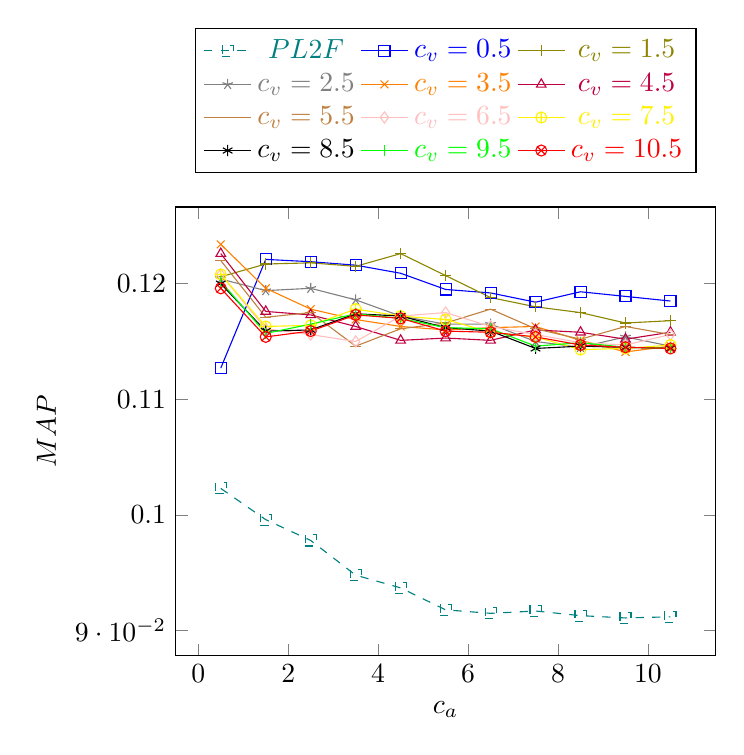
\begin{tikzpicture}
	\begin{axis}[
	  legend entries={
	    [teal]$PL2F$,
		[blue]$c_v = 0.5$,
	 	[olive]$c_v = 1.5$,
	  	[gray]$c_v = 2.5$,
	  	[orange]$c_v = 3.5$,
		[purple]$c_v = 4.5$,
	 	[brown]$c_v = 5.5$,
	  	[pink]$c_v = 6.5$,
	  	[yellow]$c_v = 7.5$,
		[black]$c_v = 8.5$,
	 	[green]$c_v = 9.5$,
	 	[red]$c_v = 10.5$
	  },
	  legend columns=3,
	legend style={at={(0.5,1.4)},anchor=north},
	 xlabel=$c_a$,
	ylabel=$MAP$,
	% y label style={rotate=-90},
	]

%%%%%%%%%%%%%%%%%%%%
%%% x=cv y=ca, from 5 to 50, with step of 5
%%%%%%%%%%%%%%%%%%%%
%\addplot[mark=square, style=solid, color=blue] coordinates
%{ (5, ) (10, ) (15, ) (20, ) (25, ) (30, ) (35, ) (40, ) (45, ) (50, )  };

%\addplot[mark=+, style=solid, color=olive] coordinates
%{ (0, 0.0928) (5, 0.1153) (10, 0.1174) (15, 0.116) (20, 0.1167) (25, 0.115) (30, 0.1136) (35, 0.1137) (40, 0.1139) (45, 0.1132) (50, 0.1136)  };

%\addplot[mark=star, style=solid, color=gray] coordinates
%{ (0, 0.0913) (5, 0.1158) (10, 0.1144) (15, 0.113) (20, 0.1136) (25, 0.114) (30, 0.1126) (35, 0.1127) (40, 0.112) (45, 0.1114) (50, 0.1106)  };

%\addplot[mark=x, style=solid, color=orange] coordinates
%{ (0, 0.0886) (5, 0.115) (10, 0.114) (15, 0.1127) (20, 0.1123) (25, 0.1123) (30, 0.1122) (35, 0.1121) (40, 0.1113) (45, 0.1105) (50, 0.1104)  };

%\addplot[mark=triangle, style=solid, color=purple] coordinates
%{ (0, 0.0879) (5, 0.114) (10, 0.1132) (15, 0.112) (20, 0.1124) (25, 0.1119) (30, 0.111) (35, 0.1111) (40, 0.1097) (45, 0.1097) (50, 0.1098)  };

%\addplot[mark=-, style=solid, color=brown] coordinates
%{ (0, 0.0868) (5, 0.1137) (10, 0.1137) (15, 0.1125) (20, 0.1111) (25, 0.1105) (30, 0.1101) (35, 0.11) (40, 0.1099) (45, 0.109) (50, 0.1091)  };

%\addplot[mark=diamond, style=solid, color=pink] coordinates
%{ (0, 0.0864) (5, 0.1131) (10, 0.1126) (15, 0.111) (20, 0.1104) (25, 0.1092) (30, 0.1092) (35, 0.1093) (40, 0.109) (45, 0.1081) (50, 0.1082)  };

%\addplot[mark=oplus, style=solid, color=yellow] coordinates
%{ (0, 0.0856) (5, 0.1129) (10, 0.1109) (15, 0.1105) (20, 0.1097) (25, 0.1084) (30, 0.1082) (35, 0.1076) (40, 0.1081) (45, 0.1079) (50, 0.107)  };

%\addplot[mark=asterisk, style=solid, color=black] coordinates
%{ (0, 0.0845) (5, 0.1124) (10, 0.1115) (15, 0.1102) (20, 0.1095) (25, 0.1083) (30, 0.1079) (35, 0.1078) (40, 0.1075) (45, 0.1073) (50, 0.1066)  };

%\addplot[mark=|, style=solid, color=green] coordinates
%{ (0, 0.0833) (5, 0.1121) (10, 0.1113) (15, 0.1099) (20, 0.1095) (25, 0.1087) (30, 0.1081) (35, 0.1081) (40, 0.1077) (45, 0.1068) (50, 0.1059)  };

%\addplot[mark=otimes, style=solid, color=red] coordinates
%{ (0, 0.0824) (5, 0.1116) (10, 0.1109) (15, 0.1099) (20, 0.1095) (25, 0.1086) (30, 0.1077) (35, 0.1077) (40, 0.1076) (45, 0.107) (50, 0.1068)  };

%%%%%%%%%%%%%%%%%%%%
%%% x=ca y=cv, from 0.5 to 10.5, with step of 1
%%%%%%%%%%%%%%%%%%%%
\addplot[mark=square, style=dashed, color=teal] coordinates
{ (0.5, 0.1023) (1.5, 0.0996) (2.5, 0.0978) (3.5, 0.0948) (4.5, 0.0937) (5.5, 0.0918) (6.5, 0.0915) (7.5, 0.0917) (8.5, 0.0913) (9.5, 0.0911) (10.5, 0.0912) };

\addplot[mark=square, style=solid, color=blue] coordinates
{ (0.5, 0.1127) (1.5, 0.1221) (2.5, 0.1219) (3.5, 0.1216) (4.5, 0.1209) (5.5, 0.1195) (6.5, 0.1192) (7.5, 0.1184) (8.5, 0.1193) (9.5, 0.1189) (10.5, 0.1185) };

\addplot[mark=+, style=solid, color=olive] coordinates
{ (0.5, 0.1206) (1.5, 0.1217) (2.5, 0.1218) (3.5, 0.1215) (4.5, 0.1226) (5.5, 0.1207) (6.5, 0.1188) (7.5, 0.118) (8.5, 0.1175) (9.5, 0.1166) (10.5, 0.1168) };

\addplot[mark=star, style=solid, color=gray] coordinates
{ (0.5, 0.1204) (1.5, 0.1194) (2.5, 0.1196) (3.5, 0.1186) (4.5, 0.1172) (5.5, 0.1165) (6.5, 0.1165) (7.5, 0.115) (8.5, 0.1145) (9.5, 0.1154) (10.5, 0.1146) };

\addplot[mark=x, style=solid, color=orange] coordinates
{ (0.5, 0.1234) (1.5, 0.1196) (2.5, 0.1178) (3.5, 0.1169) (4.5, 0.1163) (5.5, 0.116) (6.5, 0.1162) (7.5, 0.1163) (8.5, 0.1151) (9.5, 0.1141) (10.5, 0.1146) };

\addplot[mark=triangle, style=solid, color=purple] coordinates
{ (0.5, 0.1226) (1.5, 0.1176) (2.5, 0.1173) (3.5, 0.1163) (4.5, 0.1151) (5.5, 0.1153) (6.5, 0.1151) (7.5, 0.116) (8.5, 0.1158) (9.5, 0.1152) (10.5, 0.1158) };

\addplot[mark=-, style=solid, color=brown] coordinates
{ (0.5, 0.122) (1.5, 0.1171) (2.5, 0.1175) (3.5, 0.1146) (4.5, 0.1161) (5.5, 0.1166) (6.5, 0.1178) (7.5, 0.1161) (8.5, 0.1152) (9.5, 0.1163) (10.5, 0.1156) };

\addplot[mark=diamond, style=solid, color=pink] coordinates
{ (0.5, 0.1208) (1.5, 0.1161) (2.5, 0.1156) (3.5, 0.115) (4.5, 0.1172) (5.5, 0.1175) (6.5, 0.1163) (7.5, 0.1156) (8.5, 0.1149) (9.5, 0.1147) (10.5, 0.1156) };

\addplot[mark=oplus, style=solid, color=yellow] coordinates
{ (0.5, 0.1208) (1.5, 0.1163) (2.5, 0.1164) (3.5, 0.1178) (4.5, 0.1172) (5.5, 0.1169) (6.5, 0.1158) (7.5, 0.1154) (8.5, 0.1143) (9.5, 0.1144) (10.5, 0.1147) };

\addplot[mark=asterisk, style=solid, color=black] coordinates
{ (0.5, 0.12) (1.5, 0.1159) (2.5, 0.116) (3.5, 0.1174) (4.5, 0.1172) (5.5, 0.1162) (6.5, 0.1159) (7.5, 0.1144) (8.5, 0.1146) (9.5, 0.1145) (10.5, 0.1144) };

\addplot[mark=|, style=solid, color=green] coordinates
{ (0.5, 0.1202) (1.5, 0.1157) (2.5, 0.1165) (3.5, 0.1174) (4.5, 0.117) (5.5, 0.1162) (6.5, 0.1161) (7.5, 0.1146) (8.5, 0.1149) (9.5, 0.1145) (10.5, 0.1144) };

\addplot[mark=otimes, style=solid, color=red] coordinates
{ (0.5, 0.1196) (1.5, 0.1154) (2.5, 0.1159) (3.5, 0.1173) (4.5, 0.117) (5.5, 0.1159) (6.5, 0.1158) (7.5, 0.1154) (8.5, 0.1147) (9.5, 0.1145) (10.5, 0.1144) };

\end{axis}
\end{tikzpicture}}

	\caption{SS10}
\end{subfigure}
\quad%
\begin{subfigure}[b]{.3\textwidth}
	\addtocounter{subfigure}{-1}
	\renewcommand\thesubfigure{\alph{subfigure}3}
	\centering
	\resizebox{\textwidth}{!}{
	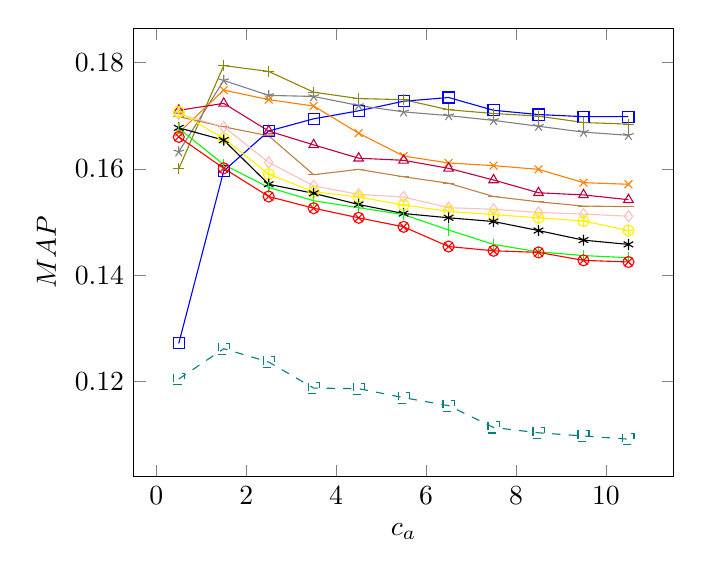
\begin{tikzpicture}
	\begin{axis}[
	 xlabel=$c_a$,
	ylabel=$MAP$,
	% y label style={rotate=-90},
	]

%%%%%%%%%%%%%%%%%%%%
%%% x=cv y=ca, from 5 to 50, with step of 5
%%%%%%%%%%%%%%%%%%%%
%%\addplot[mark=square, style=solid, color=blue] coordinates
%%{ ( , ) ( , ) ( , ) ( , ) ( , ) ( , ) ( , ) ( , ) ( , ) ( , ) ( , ) };

%\addplot[mark=+, style=solid, color=olive] coordinates
%{ (0, 0.1171) (5, 0.1608) (10 , 0.1506) (15 , 0.1448) (20 , 0.14) (25 , 0.1398) (30 , 0.139) (35 , 0.1381) (40 , 0.1371) (45 , 0.1368) (50 , 0.1361) };

%\addplot[mark=star, style=solid, color=gray] coordinates
%{ (0, 0.1098) (5 , 0.1539) (10 , 0.1436) (15 , 0.1378) (20 , 0.137) (25 , 0.1364) (30 , 0.136) (35 , 0.1351) (40 , 0.1347) (45 , 0.1342) (50 , 0.1338) };

%\addplot[mark=x, style=solid, color=orange] coordinates
%{ (0, 0.1073) (5, 0.1511) (10 , 0.1385) (15 , 0.1357) (20 , 0.1342) (25 , 0.1334) (30 , 0.1326) (35 , 0.132) (40 , 0.1312) (45 , 0.1308) (50 , 0.1282) };

%\addplot[mark=triangle, style=solid, color=purple] coordinates
%{ (0, 0.104) (5, 0.1483) (10 , 0.1365) (15 , 0.1337) (20 , 0.1327) (25 , 0.1322) (30 , 0.1312) (35 , 0.1311) (40 , 0.13) (45 , 0.1278) (50 , 0.1279) };

%\addplot[mark=-, style=solid, color=brown] coordinates
%{ (0, 0.1031) (5, 0.1464) (10 , 0.1347) (15 , 0.1327) (20 , 0.1317) (25 , 0.1314) (30 , 0.1306) (35 , 0.1302) (40 , 0.1295) (45 , 0.1274) (50 , 0.1269) };

%\addplot[mark=diamond, style=solid, color=pink] coordinates
%{ (0, 0.1024) (5, 0.1442) (10, 0.134) (15, 0.1321) (20, 0.1311) (25, 0.1309) (30, 0.1304) (35, 0.1293) (40, 0.1271) (45, 0.1268) (50, 0.1256) };

%\addplot[mark=oplus, style=solid, color=yellow] coordinates
%{ (0, 0.1019) (5, 0.1431) (10, 0.1331) (15, 0.1316) (20, 0.131) (25, 0.1304) (30, 0.1296) (35, 0.129) (40, 0.1265) (45, 0.126) (50, 0.1256) };

%\addplot[mark=asterisk, style=solid, color=black] coordinates
%{ (0, 0.1002) (5, 0.1428) (10, 0.1326) (15, 0.1311) (20, 0.1301) (25, 0.1298) (30, 0.1288) (35, 0.1285) (40, 0.1261) (45, 0.1258) (50, 0.1252) };

%\addplot[mark=|, style=solid, color=green] coordinates
%{ (0, 0.0988) (5, 0.1418) (10, 0.1322) (15, 0.1303) (20, 0.1293) (25, 0.1293) (30, 0.1284) (35, 0.1262) (40, 0.1253) (45, 0.1251) (50, 0.1247) };

%\addplot[mark=otimes, style=solid, color=red] coordinates
%{ (0, 0.0956) (5, 0.1415) (10, 0.1319) (15, 0.1301) (20, 0.129) (25, 0.1287) (30, 0.1279) (35, 0.1254) (40, 0.1251) (45, 0.1249) (50, 0.1242) };

%%%%%%%%%%%%%%%%%%%%
%%% x=ca y=cv, from 0.5 to 10.5, with step of 1
%%%%%%%%%%%%%%%%%%%%
\addplot[mark=square, style=dashed, color=teal] coordinates
{ (0.5, 0.1205) (1.5, 0.1262) (2.5, 0.1237) (3.5, 0.1188) (4.5, 0.1187) (5.5, 0.117) (6.5, 0.1155) (7.5, 0.1114) (8.5, 0.1104) (9.5, 0.1098) (10.5, 0.1092) };

\addplot[mark=square, style=solid, color=blue] coordinates
{ (0.5, 0.1272) (1.5, 0.1596) (2.5, 0.1671) (3.5, 0.1694) (4.5, 0.1709) (5.5, 0.1727) (6.5, 0.1734) (7.5, 0.171) (8.5, 0.1702) (9.5, 0.1698) (10.5, 0.1698) };

\addplot[mark=+, style=solid, color=olive] coordinates
{ (0.5, 0.16) (1.5, 0.1794) (2.5, 0.1783) (3.5, 0.1744) (4.5, 0.1732) (5.5, 0.173) (6.5, 0.1711) (7.5, 0.1704) (8.5, 0.1699) (9.5, 0.1687) (10.5, 0.1684) };

\addplot[mark=star, style=solid, color=gray] coordinates
{ (0.5, 0.1632) (1.5, 0.1766) (2.5, 0.1738) (3.5, 0.1736) (4.5, 0.1719) (5.5, 0.1707) (6.5, 0.17) (7.5, 0.1691) (8.5, 0.168) (9.5, 0.1669) (10.5, 0.1663) };

\addplot[mark=x, style=solid, color=orange] coordinates
{ (0.5, 0.1668) (1.5, 0.1748) (2.5, 0.173) (3.5, 0.1718) (4.5, 0.1667) (5.5, 0.1624) (6.5, 0.1611) (7.5, 0.1606) (8.5, 0.1599) (9.5, 0.1574) (10.5, 0.1571) };

\addplot[mark=triangle, style=solid, color=purple] coordinates
{ (0.5, 0.171) (1.5, 0.1723) (2.5, 0.1671) (3.5, 0.1645) (4.5, 0.162) (5.5, 0.1616) (6.5, 0.1601) (7.5, 0.1579) (8.5, 0.1555) (9.5, 0.1551) (10.5, 0.1542) };

\addplot[mark=-, style=solid, color=brown] coordinates
{ (0.5, 0.1698) (1.5, 0.1679) (2.5, 0.1662) (3.5, 0.1589) (4.5, 0.1599) (5.5, 0.1585) (6.5, 0.1573) (7.5, 0.1548) (8.5, 0.1538) (9.5, 0.153) (10.5, 0.1529) };

\addplot[mark=diamond, style=solid, color=pink] coordinates
{ (0.5, 0.1703) (1.5, 0.1679) (2.5, 0.1612) (3.5, 0.1568) (4.5, 0.1552) (5.5, 0.1547) (6.5, 0.1527) (7.5, 0.1524) (8.5, 0.1518) (9.5, 0.1515) (10.5, 0.1511) };

\addplot[mark=oplus, style=solid, color=yellow] coordinates
{ (0.5, 0.1707) (1.5, 0.1657) (2.5, 0.159) (3.5, 0.1557) (4.5, 0.1547) (5.5, 0.1532) (6.5, 0.152) (7.5, 0.1514) (8.5, 0.1508) (9.5, 0.1502) (10.5, 0.1484) };

\addplot[mark=asterisk, style=solid, color=black] coordinates
{ (0.5, 0.1677) (1.5, 0.1654) (2.5, 0.1571) (3.5, 0.1554) (4.5, 0.1533) (5.5, 0.1516) (6.5, 0.1508) (7.5, 0.1501) (8.5, 0.1484) (9.5, 0.1466) (10.5, 0.1458) };

\addplot[mark=|, style=solid, color=green] coordinates
{ (0.5, 0.1676) (1.5, 0.1608) (2.5, 0.1565) (3.5, 0.154) (4.5, 0.1527) (5.5, 0.1514) (6.5, 0.1485) (7.5, 0.1458) (8.5, 0.1444) (9.5, 0.1437) (10.5, 0.1433) };

\addplot[mark=otimes, style=solid, color=red] coordinates
{ (0.5, 0.166) (1.5, 0.1601) (2.5, 0.1548) (3.5, 0.1526) (4.5, 0.1508) (5.5, 0.1491) (6.5, 0.1454) (7.5, 0.1446) (8.5, 0.1443) (9.5, 0.1428) (10.5, 0.1425) };

\end{axis}
\end{tikzpicture}}

	\centering
	\caption{SS11}
\end{subfigure}

		\addtocounter{subfigure}{-1}
		\caption{Evaluation of PL2MF normalisation parameters. A curve plots a fixed $c_v$ value (Equation~(\ref{eq:pl2mf_v})) with $c_a$ (Equation~(\ref{eq:pl2mf_a})) varying from $0.5$ to $10.5$ with a precision step of $1$.}
		\label{fig:pl2mf-norm}
	\end{subfigure}
	\caption[Impact of the normalisation parameters on the MF ranking functions]{Impact of the normalisation parameters on the MF ranking functions. The figures report the MAP values of the respective datasets on the Y axis. On the X axis and with each curve, we vary the values of normalisation parameters.}
\end{figure}

\subsection{Comparison between MF and Field-Based Models}
\label{sec:mf-field-cmp}

In this section, we evaluate and compare the performance of the BM25 and PL2 ranking models against their MF extensions, BM25MF and PL2F respectively, and show the superiority of the MF model. The TF-IDF function is used as a baseline.

We outline below the ranking functions that are used in the experiments. We reuse the terminology for the equations that was presented in the previous section.

\begin{labeling}{\emph{BM25~\cite{robertson:1994:sigir}}}
  \item[\emph{TF-IDF}] is a logarithmic function of the term frequency and defines the Equation (\ref{eq:tfidf-score}) as
  $
  tfn_e=log(F_t)+1
  $,
  where $F_t$ is the number of occurrences of the term $t$ in the entity.
  \item[\emph{BM25~\cite{robertson:1994:sigir}}] considers the document as a simple bag of words. It is a function of the term frequency derived from a two-Poisson model and it uses an entity-length normalisation. The entity length is computed as the sum of the \emph{field length} defined in the Section~\ref{sec:ranking-wod}.

  It defines the Equation (\ref{eq:tfidf-score}) as
  $
  tfn_e=\frac{F_t\times(k_1+1)}{F_t+k_1\times \left(1+b\times\left(\frac{l_e}{l_{avg}}-1\right)\right)}
  $,
where $l_e$ is the \emph{entity length} of the entity $e$, $l_{avg}$ is the average of the \emph{entity length} in the collection and $b$ is a normalisation parameter.
  \item[\emph{BM25F}] is defined in Equation (\ref{eq:tfidf-score}). It considers documents as composed of fields, each field being a bag of words.
  \item[\emph{PL2~\cite{amati:2002:acm}}] considers the document as a simple bag of words. It is a model derived from the DFR framework, with the Equation (\ref{eq:pl2f}) formulated as
  $
  tfn_e=F_t\times log_2\left(1+c\times\frac{l_{avg}}{l_e}\right)
  $,
  where $c$ is a normalisation parameter.
  \item[\emph{PL2F}] is defined in Equation (\ref{eq:dfr-score}). It considers a document as a set of fields, each field being a bag of words.
\end{labeling}

The Table~\ref{tab:norm-param} reports the values of normalisation parameters for each ranking function. For a given function and dataset, the parameter value that maximises the Mean Average Precision (MAP) is found through a constrained particle swarm optimisation~\cite{xiaohui:2002:sci}. The optimisation is run on ranking functions that have all their weights equal to one, i.e., $\alpha_e = \alpha_a = \alpha_v = 1$. The reason is to limit what may impact the performance of a ranking function, thus invalidating the optimisation.\\

\begin{table}
	\centering
	\ra{0.5}
	\resizebox{\textwidth}{!}{
		\begin{tabular}{lc@{\hs}llrcllrc@{\hs}llrcllrc@{\hs}llrcllr}
			\toprule
	    & \phantom{a} & \multicolumn{7}{c}{INEX09}
	    & \phantom{a} & \multicolumn{7}{c}{SS10}
	    & \phantom{a} & \multicolumn{7}{c}{SS11} \\
	    \cmidrule{3-9} \cmidrule{11-17} \cmidrule{19-25}
			BM25MF & \phantom{a} & $b_a$ & $=$ & $0.00$ & \phantom{a} & $b_v$ & $=$ & $0.75$
	      & \phantom{a} & $b_a$ & $=$ & $0.58$ & \phantom{a} & $b_v$ & $=$ & $0.75$
	      & \phantom{a} & $b_a$ & $=$ & $0.58$ & \phantom{a} & $b_v$ & $=$ & $0.75$ \\
			BM25 & \phantom{a} & $b$ & $=$ & $0.20$ & \multicolumn{4}{c}{\phantom{a}}
	    & \phantom{a} & $b$ & $=$ & $0.20$ & \multicolumn{4}{c}{\phantom{a}}
	    & \phantom{a} & $b$ & $=$ & $0.20$ & \multicolumn{4}{c}{\phantom{a}} \\
			BM25F & \phantom{a} & $b_a$ & $=$ & $0.82$ & \multicolumn{4}{c}{\phantom{a}}
	     & \phantom{a} & $b_a$ & $=$ & $0.82$ & \multicolumn{4}{c}{\phantom{a}}
	     & \phantom{a} & $b_a$ & $=$ & $0.82$ & \multicolumn{4}{c}{\phantom{a}} \\
			\midrule
			PL2MF & \phantom{a} & $c_a$ & $=$ & $9.19$ & \phantom{a} & $c_v$ & $=$ & $0.76$
	     & \phantom{a} & $c_a$ & $=$ & $1.52$ & \phantom{a} & $c_v$ & $=$ & $1.03$
	     & \phantom{a} & $c_a$ & $=$ & $1.79$ & \phantom{a} & $c_v$ & $=$ & $1.88$ \\
			PL2 & \phantom{a} & $c$ & $=$ & $17.01$ & \multicolumn{4}{c}{\phantom{a}}
	   & \phantom{a} & $c$ & $=$ & $10.09$ & \multicolumn{4}{c}{\phantom{a}}
	   & \phantom{a} & $c$ & $=$ & $10.09$ & \multicolumn{4}{c}{\phantom{a}} \\
			PL2F & \phantom{a} & $c_a$ & $=$ & $1.87$ & \multicolumn{4}{c}{\phantom{a}}
	     & \phantom{a} & $c_a$ & $=$ & $0.51$ & \multicolumn{4}{c}{\phantom{a}}
	     & \phantom{a} & $c_a$ & $=$ & $1.51$ & \multicolumn{4}{c}{\phantom{a}} \\
			\bottomrule
		\end{tabular}
	}
	\caption{Normalization parameters values, found through a constrained particle swarm optimization.}
	\label{tab:norm-param}
\end{table}


Using such parameters, we report in Figures~\ref{fig:bm25mf-field-cmp-bar}~and~\ref{fig:pl2mf-field-cmp-bar} the performance of the ranking functions on the three datasets, for BM25MF and PL2MF respectively. The raw results of the bar charts are available in the Appendix section, in Table~\ref{tab:ranking-cmp-results}.

Using the two-tailed Wilcoxon matched-pairs signed-ranks test~\cite{sheskin:2003:CRC,buttcher:2010:IRI:1869919}, the difference between a candidate ranking function and a MF extension is statistically significant at level $0.05$ if the bar is displayed with a \textit{dot} pattern; it is statistically significant at level $0.10$ if displayed with a \emph{oblique lines} pattern instead.\\

%We note that for field-based ranking models and their MF extensions, the attribute label is considered as a value node, in order to be a source of potential relevant terms.
TF-IDF provides a clear-cut discrepancy between INEX09 and the datasets based on BTC, i.e., SS10 and SS11, the reason being it is not suited for heterogeneous datasets.

On SS10, BM25MF (resp., PL2MF) does not report a significant difference with BM25 (resp., PL2). On INEX09 and SS11, the MF extensions provide an increase of at least $10\%$ in retrieval performance compared to BM25 and PL2.

On SS10 and SS11, the MF extensions provide better ranking performance with a significant difference than the field-based ranking functions with an increase of $15\%$ at the minimum. On INEX09, PL2F and its MF extension PL2MF provide similar ranking performance.

Overall, the experiments show that the MF model improves significantly the ranking effectiveness over traditional field-based methods. In addition, the experiments emphasize as well the fine tuning possible with the MF ranking model, allowing to better fit the ranking to a specific dataset.

\begin{figure}
	\centering
	\begin{subfigure}{.47\textwidth}
		\centering
		\resizebox{\textwidth}{!}{
			\begin{tikzpicture}
			\begin{axis}[
			ybar,
			symbolic x coords={TF-IDF,BM25,BM25F,BM25MF},
			enlargelimits=0.15,
			ylabel={MAP},
			x=2cm,
			bar width=0.3cm,
			xtick=data,
			ymajorgrids = true,
			legend style={at={(0.5,-0.15)}, anchor=north,legend columns=-1},
			legend entries={INEX09,SS10,SS11}
			]
			% These plots are here only to the set the style
			\addplot[blue, fill=blue!20, bar shift=-0.45cm] coordinates {
				(TF-IDF, 0.04)
				(BM25, 0.04)
				(BM25F, 0.04)
				(BM25MF, 0.04)
			};
			\addplot[red, fill=red!20, bar shift=0cm] coordinates {
				(TF-IDF, 0.04)
				(BM25, 0.04)
				(BM25F, 0.04)
				(BM25MF, 0.04)
			};
			\addplot[brown, fill=brown!20, bar shift=0.45cm] coordinates {
				(TF-IDF, 0.04)
				(BM25, 0.04)
				(BM25F, 0.04)
				(BM25MF, 0.04)
			};

			% INEX09
			\addplot[blue, fill=blue!20, bar shift=-0.45cm] coordinates {
				(BM25MF, 0.1593)
			};
			\addplot[blue, fill=blue!20, postaction={pattern=crosshatch dots}, bar shift=-0.45cm] coordinates {
				(TF-IDF, 0.1246)
				(BM25, 0.1330)
				(BM25F, 0.1489)
			};
			% SS10
			\addplot[red, fill=red!20, bar shift=0cm] coordinates {
				(BM25, 0.1350)
				(BM25MF, 0.1303)
			};
			\addplot[red, fill=red!20, postaction={pattern=crosshatch dots}, bar shift=0cm] coordinates {
				(TF-IDF, 0.0581)
				(BM25F, 0.1100)
			};
			% SS11
			\addplot[brown, fill=brown!20, bar shift=0.45cm] coordinates {
				(BM25MF, 0.1811)
			};
			\addplot[brown, fill=brown!20, postaction={pattern=crosshatch dots}, bar shift=0.45cm] coordinates {
				(TF-IDF, 0.0655)
				(BM25F, 0.1401)
			};
			\addplot[brown, fill=brown!20, postaction={pattern=north east lines}, bar shift=0.45cm] coordinates {
				(BM25, 0.1625)
			};
			\end{axis}
			\end{tikzpicture}
		}
		\caption{BM25MF}
		\label{fig:bm25mf-field-cmp-bar}
	\end{subfigure}
	\quad
	\begin{subfigure}{.47\textwidth}
		\centering
		\resizebox{\textwidth}{!}{
			\begin{tikzpicture}
			\begin{axis}[
				ybar,
				symbolic x coords={TF-IDF,PL2,PL2F,PL2MF},
				enlargelimits=0.15,
				ylabel={MAP},
				x=2cm,
				bar width=0.3cm,
				xtick=data,
				ymajorgrids = true,
				legend style={at={(0.5,-0.15)}, anchor=north,legend columns=-1},
				legend entries={INEX09,SS10,SS11}
			]
			% These plots are here only to the set the style
			\addplot[blue, fill=blue!20, bar shift=-0.45cm] coordinates {
				(TF-IDF, 0.04)
				(PL2, 0.04)
				(PL2F, 0.04)
				(PL2MF, 0.04)
			};
			\addplot[red, fill=red!20, bar shift=0cm] coordinates {
				(TF-IDF, 0.04)
				(PL2, 0.04)
				(PL2F, 0.04)
				(PL2MF, 0.04)
			};
			\addplot[brown, fill=brown!20, bar shift=0.45cm] coordinates {
				(TF-IDF, 0.04)
				(PL2, 0.04)
				(PL2F, 0.04)
				(PL2MF, 0.04)
			};

			% INEX09
			\addplot[blue, fill=blue!20, bar shift=-0.45cm] coordinates {
				(PL2F, 0.1514)
				(PL2MF, 0.1525)
			};
			\addplot[blue, fill=blue!20, postaction={pattern=crosshatch dots}, bar shift=-0.45cm] coordinates {
				(TF-IDF, 0.1246)
				(PL2, 0.1331)
			};
			% SS10
			\addplot[red, fill=red!20, bar shift=0cm] coordinates {
				(PL2, 0.1289)
				(PL2MF, 0.1232)
			};
			\addplot[red, fill=red!20, postaction={pattern=crosshatch dots}, bar shift=0cm] coordinates {
				(TF-IDF, 0.0581)
				(PL2F, 0.1023)
			};
			% SS11
			\addplot[brown, fill=brown!20, bar shift=0.45cm] coordinates {
				(PL2MF, 0.1797)
			};
			\addplot[brown, fill=brown!20, postaction={pattern=crosshatch dots}, bar shift=0.45cm] coordinates {
				(TF-IDF, 0.0655)
				(PL2F, 0.1264)
			};
			\addplot[brown, fill=brown!20, postaction={pattern=north east lines}, bar shift=0.45cm] coordinates {
				(PL2, 0.1614)
			};
			\end{axis}
			\end{tikzpicture}
		}
		\caption{PL2MF}
		\label{fig:pl2mf-field-cmp-bar}
	\end{subfigure}
	\caption[Comparison of state-of-the-art ranking functions against the MF generalizations]{Comparison of state-of-the-art candidates against the MF generalizations. On the Y axis is reported the Mean Average Precision of the MF extensions and the other state-of-the-art candidates. Bars with a dot pattern indicate a statistically significant difference at level $0.05$ compared to the MF extension; bars with a oblique lines pattern is at level $0.10$ instead.}
\end{figure}


\subsection{Effectiveness of the Weights}
\label{sec:weights-effectiveness}

In this section, we evaluate the impact of the presented weights over the MF ranking extensions. First, we discuss the impact of discarding the attribute label as a source of possible relevant terms on the ranking performance. Then, we evaluate the weights from Section~\ref{sec:weights} developed for the MF model.

Results of the evaluations are depicted in Figure~\ref{fig:mf-weights}. The PL2MF results are displayed on the left side of the figures, and on the right side the results of BM25MF. Using the two-tailed Wilcoxon matched-pairs signed-ranks test~\cite{sheskin:2003:CRC,buttcher:2010:IRI:1869919}, the MF extension with no added weight is used as the base of the comparison. Bars with a dot pattern indicate a statistically significant difference at level $0.05$ compared to the MF extension; bars with a oblique lines pattern is at level $0.10$ instead. Raw results are reported in Table~\ref{tab:mf-effect} of the Appendix section.

\subsubsection{\emph{Impact of the Attribute Label}}
\label{sec:with-att}

In this section, we investigate the consequence of \textbf{not} considering the attribute label as a source of potentially relevant terms, i.e., the attribute is not expanded into a leaf as described in Section~\ref{chap:tree-ranking:mf-model}.

Figure~\ref{fig:mf-att} depicts the results, where we observe that removing the attribute label lowers the performance of the ranking with a statistical significance on INEX09 with BM25MF and PL2MF, and on SS11 with PL2MF only. This shows that the attribute labels can be a source of possible relevant terms.

\subsubsection{\emph{Query Coverage Weight}}
\label{sec:qc-weight-effect}

In order to evaluate the benefit of the query coverage weight QC, we first analyse its effect separately when applied as an entity, an attribute or a value-specific weight. Then we study the consequence of applying it on all nodes at the same time.

We observe in Figure~\ref{fig:mf-qc} that the QC weight improves the retrieval performance when applied on the attribute node, with a statistical significance on SS10 and SS11.

\subsubsection{\emph{Leaf Coverage Weight}}
\label{sec:lc-weight-effect}

The evaluation of the leaf coverage weight LC investigates its efficiency with and without the \emph{control} function (\ref{eq:lc-norm}), where we depict the results in Figure~\ref{fig:mf-lc}.

We provide for each dataset the best performing parameters described in Section~\ref{sec:leaf-coverage} for the control function. For the three datasets regardless of the MF extension, the values are as follows:
\begin{description}
	\item[INEX09:] $n=1\;\;\alpha=0.7$;
	\item[SS10:] $n=2\;\;\alpha=0.4$; and
	\item[SS11:] $n=1\;\;\alpha=0.9$.
\end{description}
We can observe that the LC weight, with the control function (\ref{eq:lc-norm}) applied, improves slightly the retrieval performance on SS10 and SS11. The reason is that without this function, LC assigns a low weight to leaves containing many terms, even if they have occurrences of all query terms.

\subsubsection{\emph{Attribute and Entity Labels Weights}}
\label{sec:ael-weight-effect}

For the weights that depend on the label of the entity or of an attribute, we use the following regular expressions to determine the value of the weight:
\begin{itemize}
	\item $2$ if the label matches "\verb/.*(label|name|title|sameas)$/";
	\item $0.5$ if the label matches "\verb/.*(seealso|wikilinks)$/";
	\item $0.1$ if the label matches "\verb|^http://www.w3.org/1999/02/22-rdf-syntax-ns#_\d+$|"; and
	\item $1$ otherwise.
\end{itemize}
For instance, if an attribute label is \url{http://xmlns.com/foaf/0.1/name} then a weight of $2$ is assigned. The weight's values are set empirically, and were chosen in order to improve the task of entity search. The rationale is that a document where a query term occurs associated with an attribute matching "title\$" should be promoted.

The third regular expression matches an attribute URI defining items of a collection in RDF\footnote{RDF Container: \url{http://www.w3.org/TR/rdf-schema/\#ch\_container}}. It is assigned a low weight of $0.1$ to reduce the importance of terms occurring in each item of the collection.\\

We evaluate the Attribute and Entity Labels (AEL) weights first by considering the Attribute and the Entity Label weights separately, then both at the same time. Figure~\ref{fig:mf-ael} depicts the results of applying such query-independent weights.

We note that the Attribute Label weight gives significant benefits to the ranking in SS10 and SS11, while it decreases the ranking performance in INEX09. This indicates that carefully defined weights for important and non-important attributes can contribute significantly to the effectiveness of the approach. We note also that the same can be seen with the Entity Label weight applied alone. The reason is similar to the Attribute Label weight.

Except for INEX09, using both weights at the same time increases the performance of MF ranking functions noticeably.

\subsubsection{\emph{Combination of Weights}}
\label{sec:combi-weight-effect}

In this section, we investigate the retrieval performance when all four weights are used together. We depict results in Figure~\ref{fig:mf-all}, with the weights configuration
\begin{enumerate}
    \item QC applied on the attribute node only;
    \item LC with dataset-specific $n$ and $\alpha$ parameters for the control function; and
    \item AEL weights.
\end{enumerate}

The weights applied on a same node are combined by the multiplication of each weight value on that node.
The attribute and entity label being leaves in the ranking model, we apply also the QC weight on those two in this experiment.

On INEX09 their combination decreases slightly the performance for PL2MF. On SS10 and SS11, although the QC and LC weights applied separately do not improve the effectiveness of the MF ranking functions by much, their combination with AEL increases the retrieval performance by at least $30\%$ on SS10 and SS11.

\begin{figure}
	\centering
	\begin{subfigure}{.483\textwidth}
		\centering
		\resizebox{\textwidth}{!}{
			%\begin{tikzpicture}
%\begin{axis}[
%	ybar,
%	symbolic x coords={INEX09,SS10,SS11},
%	enlargelimits=0.15,
%	ylabel={MAP},
%	x=2cm,
%	bar width=0.3cm,
%	xtick=data,
%	ymajorgrids = true,
%	legend style={at={(0.5,-0.15)}, anchor=north,legend columns=-1},
%	legend entries={With Attribute, Without Attribute}
%]
%% These plots are here only to the set the style
%\addplot[blue, fill=blue!20, bar shift=-0.15cm] coordinates {
%	(INEX09, 0.04)
%	(SS10, 0.04)
%	(SS11, 0.04)
%};
%\addplot[red, fill=red!20, bar shift=0.3cm] coordinates {
%	(INEX09, 0.04)
%	(SS10, 0.04)
%	(SS11, 0.04)
%};
%
%\addplot[blue, fill=blue!20, bar shift=-0.15cm] coordinates {
%	(INEX09, 0.1593)
%	(SS10, 0.1303)
%	(SS11, 0.1811)
%};
%\addplot[red, fill=red!20, bar shift=0.3cm] coordinates {
%	(SS10, 0.1241)
%	(SS11, 0.1763)
%};
%\addplot[red, fill=red!20, postaction={pattern=crosshatch dots}, bar shift=0.3cm] coordinates {
%	(INEX09, 0.1484)
%};
%\end{axis}
%\end{tikzpicture}



\begin{tikzpicture}
\begin{axis}[
xticklabel pos=right,
name=bm25mf,
xbar,
enlargelimits=0.15,
xlabel={MAP},
y=2cm,
bar width=0.35cm,
ytick=data,
xmajorgrids = true,
legend style={at={(0.5,-0.02)}, anchor=north,legend columns=-1},
legend entries={BM25MF,Without},
axis y line=none,
clip=false
]
% These plots are here only to the set the style
\addplot[blue, fill=blue!20, bar shift=-0.15cm] coordinates {
	(0.1241, 1)
	(0.1241, 2)
	(0.1241, 3)
};
\addplot[red, fill=red!20, bar shift=0.3cm] coordinates {
	(0.1241, 1)
	(0.1241, 2)
	(0.1241, 3)
};

\addplot[blue, fill=blue!20, bar shift=-0.15cm] coordinates {
	(0.1593, 1)
	(0.1303, 2)
	(0.1811, 3)
};
\addplot[red, fill=red!20, bar shift=0.3cm] coordinates {
	(0.1241, 2)
	(0.1763, 3)
};
\addplot[red, fill=red!20, postaction={pattern=crosshatch dots}, bar shift=0.3cm] coordinates {
	(0.1484, 1)
};
\node[xshift=-0.35cm,align=center] at (axis cs:0.11,1) {INEX09};
\node[xshift=-0.35cm,align=center] at (axis cs:0.11,2) {SS10};
\node[xshift=-0.35cm,align=center] at (axis cs:0.11,3) {SS11};
\end{axis}
\begin{axis}[
xticklabel pos=right,
legend style={at={(0.5,-0.02)}, anchor=north,legend columns=-1},
legend entries={PL2MF,Without},
at={(bm25mf.north west)},anchor=north east, xshift=-1.7cm,
x dir = reverse,
xbar,
enlargelimits=0.15,
xlabel={MAP},
y=2cm,
bar width=0.35cm,
ytick=data,
xmajorgrids = true,
axis y line=none
]
% These plots are here only to the set the style
\addplot[blue, fill=blue!20, bar shift=-0.15cm] coordinates {
	(0.1192, 1)
	(0.1192, 2)
	(0.1192, 3)
};
\addplot[red, fill=red!20, bar shift=0.3cm] coordinates {
	(0.1192, 1)
	(0.1192, 2)
	(0.1192, 3)
};

\addplot[blue, fill=blue!20, bar shift=-0.15cm] coordinates {
	(0.1525, 1)
	(0.1232, 2)
	(0.1797, 3)
};
\addplot[red, fill=red!20, bar shift=0.3cm] coordinates {
	(0.1192, 2)
};
\addplot[red, fill=red!20, postaction={pattern=north east lines}, bar shift=0.3cm] coordinates {
	(0.1680, 3)
};
\addplot[red, fill=red!20, postaction={pattern=crosshatch dots}, bar shift=0.3cm] coordinates {
	(0.1401, 1)
};
\end{axis}
\end{tikzpicture}

		}
		\caption{Without the attribute as a leaf}
		\label{fig:mf-att}
	\end{subfigure}
	\quad
	\begin{subfigure}{.483\textwidth}
		\centering
		\resizebox{\textwidth}{!}{
			%\begin{tikzpicture}
%\begin{axis}[
%	ybar,
%	symbolic x coords={INEX09,SS10,SS11},
%	enlargelimits=0.2,
%	ylabel={MAP},
%	x=3cm,
%	bar width=0.3cm,
%	xtick=data,
%	ymajorgrids = true,
%	legend style={at={(0.5,-0.15)}, anchor=north,legend columns=-1},
%	legend entries={No QC, QC on Leaf, QC on Attribute, QC on Entity, All},
%]
%% These plots are here only to the set the style
%\addplot[blue, fill=blue!20, bar shift=-0.90cm] coordinates {
%	(INEX09, 0.04)
%	(SS10, 0.04)
%	(SS11, 0.04)
%};
%\addplot[red, fill=red!20, bar shift=-0.45cm] coordinates {
%	(INEX09, 0.04)
%	(SS10, 0.04)
%	(SS11, 0.04)
%};
%\addplot[brown, fill=brown!20, bar shift=0cm] coordinates {
%	(INEX09, 0.04)
%	(SS10, 0.04)
%	(SS11, 0.04)
%};
%\addplot[green, fill=green!20, bar shift=0.45cm] coordinates {
%	(INEX09, 0.04)
%	(SS10, 0.04)
%	(SS11, 0.04)
%};
%\addplot[black, fill=black!20, bar shift=0.90cm] coordinates {
%	(INEX09, 0.04)
%	(SS10, 0.04)
%	(SS11, 0.04)
%};
%
%% Baseline: BM25MF + attribute label
%\addplot[blue, fill=blue!20, bar shift=-0.90cm] coordinates {
%	(INEX09, 0.1593)
%	(SS10, 0.1303)
%	(SS11, 0.1811)
%};
%% QC on Value
%\addplot[red, fill=red!20, bar shift=-0.45cm] coordinates {
%	(SS10, 0.1325)
%};
%\addplot[red, fill=red!20, postaction={pattern=north east lines}, bar shift=-0.45cm] coordinates {
%	(INEX09, 0.1482)
%	(SS11, 0.1841)
%};
%% QC on attribute
%\addplot[brown, fill=brown!20, bar shift=0cm] coordinates {
%	(INEX09, 0.1624)
%};
%\addplot[brown, fill=brown!20, postaction={pattern=north east lines}, bar shift=0cm] coordinates {
%	(SS10, 0.1339)
%	(SS11, 0.1841)
%};
%% QC on Entity
%\addplot[green, fill=green!20, bar shift=0.45cm] coordinates {
%	(SS11, 0.1744)
%};
%\addplot[green, fill=green!20, postaction={pattern=north east lines}, bar shift=0.45cm] coordinates {
%	(INEX09, 0.1514)
%};
%\addplot[green, fill=green!20, postaction={pattern=crosshatch dots}, bar shift=0.45cm] coordinates {
%	(SS10, 0.1236)
%};
%% QC with all
%\addplot[black, fill=black!20, bar shift=0.90cm] coordinates {
%	(SS11, 0.1810)
%};
%\addplot[black, fill=black!20, postaction={pattern=north east lines}, bar shift=0.90cm] coordinates {
%	(INEX09, 0.1506)
%	(SS10, 0.1263)
%};
%\end{axis}
%\end{tikzpicture}







\begin{tikzpicture}
\begin{axis}[
xticklabel pos=right,
name=bm25mf,
xbar,
enlargelimits=0.22,
xlabel={MAP},
y=3cm,
bar width=0.35cm,
ytick=data,
xmajorgrids = true,
legend style={at={(0.5,-0.02)}, anchor=north,legend columns=-1},
legend entries={BM25MF,Leaf, Attribute, Entity, All},
axis y line=none,
clip=false
]
% These plots are here only to the set the style
\addplot[blue, fill=blue!20, bar shift=-0.90cm] coordinates {
	(0.1236, 1)
	(0.1236, 1)
	(0.1236, 1)
};
\addplot[red, fill=red!20, bar shift=-0.45cm] coordinates {
	(0.1236, 1)
	(0.1236, 1)
	(0.1236, 1)
};
\addplot[brown, fill=brown!20, bar shift=0cm] coordinates {
	(0.1236, 1)
	(0.1236, 1)
	(0.1236, 1)
};
\addplot[green, fill=green!20, bar shift=0.45cm] coordinates {
	(0.1236, 1)
	(0.1236, 1)
	(0.1236, 1)
};
\addplot[black, fill=black!20, bar shift=0.90cm] coordinates {
	(0.1236, 1)
	(0.1236, 1)
	(0.1236, 1)
};

% Baseline: BM25MF + attribute label
\addplot[blue, fill=blue!20, bar shift=-0.90cm] coordinates {
	(0.1593, 1)
	(0.1303, 2)
	(0.1811, 3)
};
% QC on Value
\addplot[red, fill=red!20, bar shift=-0.45cm] coordinates {
	(0.1325, 2)
};
\addplot[red, fill=red!20, postaction={pattern=north east lines}, bar shift=-0.45cm] coordinates {
	(0.1482, 1)
	(0.1841, 3)
};
% QC on attribute
\addplot[brown, fill=brown!20, bar shift=0cm] coordinates {
	(0.1624, 1)
};
\addplot[brown, fill=brown!20, postaction={pattern=north east lines}, bar shift=0cm] coordinates {
	(0.1339, 2)
	(0.1841, 3)
};
% QC on Entity
\addplot[green, fill=green!20, bar shift=0.45cm] coordinates {
	(0.1744, 3)
};
\addplot[green, fill=green!20, postaction={pattern=north east lines}, bar shift=0.45cm] coordinates {
	(0.1514, 1)
};
\addplot[green, fill=green!20, postaction={pattern=crosshatch dots}, bar shift=0.45cm] coordinates {
	(0.1236, 2)
};
% QC with all
\addplot[black, fill=black!20, bar shift=0.90cm] coordinates {
	(0.1810, 3)
};
\addplot[black, fill=black!20, postaction={pattern=north east lines}, bar shift=0.90cm] coordinates {
	(0.1506, 1)
	(0.1263, 2)
};
\node[xshift=-0.8cm,align=center] at (axis cs:0.11,1) {INEX09};
\node[xshift=-0.8cm,align=center] at (axis cs:0.11,2) {SS10};
\node[xshift=-0.8cm,align=center] at (axis cs:0.11,3) {SS11};
\end{axis}
\begin{axis}[
xticklabel pos=right,
legend style={at={(0.5,-0.02)}, anchor=north,legend columns=-1},
legend entries={PL2MF,Leaf, Attribute, Entity, All},
at={(bm25mf.north west)},anchor=north east, xshift=-1.7cm,
x dir = reverse,
xbar,
enlargelimits=0.22,
xlabel={MAP},
y=3cm,
bar width=0.35cm,
ytick=data,
xmajorgrids = true,
axis y line=none
]
% These plots are here only to the set the style
\addplot[blue, fill=blue!20, bar shift=-0.90cm] coordinates {
	(0.1168, 1)
	(0.1168, 1)
	(0.1168, 1)
};
\addplot[red, fill=red!20, bar shift=-0.45cm] coordinates {
	(0.1168, 1)
	(0.1168, 1)
	(0.1168, 1)
};
\addplot[brown, fill=brown!20, bar shift=0cm] coordinates {
	(0.1168, 1)
	(0.1168, 1)
	(0.1168, 1)
};
\addplot[green, fill=green!20, bar shift=0.45cm] coordinates {
	(0.1168, 1)
	(0.1168, 1)
	(0.1168, 1)
};
\addplot[black, fill=black!20, bar shift=0.90cm] coordinates {
	(0.1168, 1)
	(0.1168, 1)
	(0.1168, 1)
};

% PL2MF
\addplot[blue, fill=blue!20, bar shift=-0.90cm] coordinates {
	(0.1525, 1)
	(0.1232, 2)
	(0.1797, 3)
};
% QC on leaf
\addplot[red, fill=red!20, postaction={pattern=crosshatch dots}, bar shift=-0.45cm] coordinates {
	(0.1348, 1)
};
\addplot[red, fill=red!20, postaction={pattern=north east lines}, bar shift=-0.45cm] coordinates {
	(0.1276, 2)
	(0.1818, 3)
};
% QC on attribute
\addplot[brown, fill=brown!20, bar shift=0cm] coordinates {
	(0.1569, 1)
};
\addplot[brown, fill=brown!20, postaction={pattern=north east lines}, bar shift=0cm] coordinates {
	(0.1299, 2)
	(0.1815, 3)
};
% QC on entity
\addplot[green, fill=green!20, bar shift=0.45cm] coordinates {
	(0.1499, 1)
};
\addplot[green, fill=green!20, postaction={pattern=crosshatch dots}, bar shift=0.45cm] coordinates {
	(0.1168, 2)
};
\addplot[green, fill=green!20, postaction={pattern=north east lines}, bar shift=0.45cm] coordinates {
	(0.1655, 3)
};
% QC on all
\addplot[black, fill=black!20, bar shift=0.90cm] coordinates {
	(0.1257, 2)
	(0.1743, 3)
};
\addplot[black, fill=black!20, postaction={pattern=crosshatch dots}, bar shift=0.90cm] coordinates {
	(0.1374, 1)
};
\end{axis}
\end{tikzpicture}

		}
		\caption{Query coverage weight QC applied on the leaf, on the attribute, on the entity, and on all three levels}
		\label{fig:mf-qc}
	\end{subfigure}
	\qquad
	\begin{subfigure}{.483\textwidth}
		\centering
		\resizebox{\textwidth}{!}{
			%\begin{tikzpicture}
%\begin{axis}[
%	ybar,
%	symbolic x coords={INEX09,SS10,SS11},
%	enlargelimits=0.2,
%	ylabel={MAP},
%	x=2cm,
%	bar width=0.3cm,
%	xtick=data,
%	ymajorgrids = true,
%	legend style={at={(0.5,-0.15)}, anchor=north,legend columns=-1},
%	legend entries={BM25MF,With,Without},
%]
%% These plots are here only to the set the style
%\addplot[blue, fill=blue!20, bar shift=-0.45cm] coordinates {
%	(INEX09, 0.04)
%	(SS10, 0.04)
%	(SS11, 0.04)
%};
%\addplot[red, fill=red!20, bar shift=0cm] coordinates {
%	(INEX09, 0.04)
%	(SS10, 0.04)
%	(SS11, 0.04)
%};
%\addplot[brown, fill=brown!20, bar shift=0.45cm] coordinates {
%	(INEX09, 0.04)
%	(SS10, 0.04)
%	(SS11, 0.04)
%};
%
%% Baseline: BM25MF + attribute label
%\addplot[blue, fill=blue!20, bar shift=-0.45cm] coordinates {
%	(INEX09, 0.1593)
%	(SS10,   0.1303)
%	(SS11,   0.1811)
%};
%% LC with control function
%\addplot[red, fill=red!20, bar shift=0cm] coordinates {
%	(INEX09, 0.1606)
%	(SS10,   0.1321)
%	(SS11,   0.1802)
%};
%\addplot[red, fill=red!20, postaction={pattern=north east lines}, bar shift=0cm] coordinates {
%	(INEX09, 0.1606)
%};
%% LC without control function
%\addplot[brown, fill=brown!20, bar shift=0.45cm] coordinates {
%	(SS10,   0.1260)
%};
%\addplot[brown, fill=brown!20, postaction={pattern=crosshatch dots}, bar shift=0.45cm] coordinates {
%	(INEX09, 0.1293)
%	(SS11,   0.1296)
%};
%\end{axis}
%\end{tikzpicture}



\begin{tikzpicture}
\begin{axis}[
xticklabel pos=right,
name=bm25mf,
xbar,
enlargelimits=0.2,
xlabel={MAP},
y=2.2cm,
bar width=0.35cm,
ytick=data,
xmajorgrids = true,
legend style={at={(0.5,-0.02)}, anchor=north,legend columns=-1},
legend entries={BM25MF,With,Without},
axis y line=none,
clip=false
]
% These plots are here only to the set the style
\addplot[blue, fill=blue!20, bar shift=-0.45cm] coordinates {
	(0.1260, 1)
	(0.1260, 1)
	(0.1260, 1)
};
\addplot[red, fill=red!20, bar shift=0cm] coordinates {
	(0.1260, 1)
	(0.1260, 2)
	(0.1260, 3)
};
\addplot[brown, fill=brown!20, bar shift=0.45cm] coordinates {
	(0.1260, 1)
	(0.1260, 2)
	(0.1260, 3)
};

% Baseline: BM25MF + attribute label
\addplot[blue, fill=blue!20, bar shift=-0.45cm] coordinates {
	(0.1593, 1)
	(0.1303, 2)
	(0.1811, 3)
};
% LC with control function
\addplot[red, fill=red!20, bar shift=0cm] coordinates {
	(0.1321, 2)
	(0.1802, 3)
};
\addplot[red, fill=red!20, postaction={pattern=north east lines}, bar shift=0cm] coordinates {
	(0.1606, 1)
};
% LC without control function
\addplot[brown, fill=brown!20, bar shift=0.45cm] coordinates {
	(0.1260, 2)
};
\addplot[brown, fill=brown!20, postaction={pattern=crosshatch dots}, bar shift=0.45cm] coordinates {
	(0.1293, 1)
	(0.1296, 3)
};
\node[xshift=-0.4cm,align=center] at (axis cs:0.11,1) {INEX09};
\node[xshift=-0.4cm,align=center] at (axis cs:0.11,2) {SS10};
\node[xshift=-0.4cm,align=center] at (axis cs:0.11,3) {SS11};
\end{axis}
\begin{axis}[
xticklabel pos=right,
legend style={at={(0.5,-0.02)}, anchor=north,legend columns=-1},
legend entries={PL2MF,With,Without},
at={(bm25mf.north west)},anchor=north east, xshift=-1.7cm,
x dir = reverse,
xbar,
enlargelimits=0.2,
xlabel={MAP},
y=2.2cm,
bar width=0.35cm,
ytick=data,
xmajorgrids = true,
axis y line=none
]
% These plots are here only to the set the style
\addplot[blue, fill=blue!20, bar shift=-0.45cm] coordinates {
	(0.1179, 1)
	(0.1179, 1)
	(0.1179, 1)
};
\addplot[red, fill=red!20, bar shift=0cm] coordinates {
	(0.1179, 1)
	(0.1179, 2)
	(0.1179, 3)
};
\addplot[brown, fill=brown!20, bar shift=0.45cm] coordinates {
	(0.1179, 1)
	(0.1179, 2)
	(0.1179, 3)
};

% Baseline: PL2MF + attribute label
\addplot[blue, fill=blue!20, bar shift=-0.45cm] coordinates {
	(0.1525, 1)
	(0.1232, 2)
	(0.1797, 3)
};
% LC with control function
\addplot[red, fill=red!20, postaction={pattern=crosshatch dots}, bar shift=0cm] coordinates {
	(0.1494, 1)
};
\addplot[red, fill=red!20, postaction={pattern=north east lines}, bar shift=0cm] coordinates {
	(0.1253, 2)
	(0.1802, 3)
};
% LC without control function
\addplot[brown, fill=brown!20, bar shift=0.45cm] coordinates {
	(0.1179, 2)
};
\addplot[brown, fill=brown!20, postaction={pattern=crosshatch dots}, bar shift=0.45cm] coordinates {
	(0.1182, 1)
	(0.1466, 3)
};
\end{axis}
\end{tikzpicture}

		}
		\caption{Leaf coverage weight LC, tested with and without the control function in Equation~(\ref{eq:lc-norm})}
		\label{fig:mf-lc}
	\end{subfigure}
	\quad
	\begin{subfigure}{.483\textwidth}
		\centering
		\resizebox{\textwidth}{!}{
			%\begin{tikzpicture}
%\begin{axis}[
%	ybar,
%	symbolic x coords={INEX09,SS10,SS11},
%	enlargelimits=0.2,
%	ylabel={MAP},
%	x=2.5cm,
%	bar width=0.3cm,
%	xtick=data,
%	ymajorgrids = true,
%	legend style={at={(0.5,-0.15)}, anchor=north,legend columns=-1},
%	legend entries={BM25MF,Entity,Attribute,All},
%]
%% These plots are here only to the set the style
%\addplot[blue, fill=blue!20, bar shift=-0.675cm] coordinates {
%	(INEX09, 0.04)
%	(SS10, 0.04)
%	(SS11, 0.04)
%};
%\addplot[red, fill=red!20, bar shift=-0.225cm] coordinates {
%	(INEX09, 0.04)
%	(SS10, 0.04)
%	(SS11, 0.04)
%};
%\addplot[brown, fill=brown!20, bar shift=0.225cm] coordinates {
%	(INEX09, 0.04)
%	(SS10, 0.04)
%	(SS11, 0.04)
%};
%\addplot[black, fill=black!20, bar shift=0.675cm] coordinates {
%	(INEX09, 0.04)
%	(SS10, 0.04)
%	(SS11, 0.04)
%};
%
%% Baseline: BM25MF + attribute label
%\addplot[blue, fill=blue!20, bar shift=-0.675cm] coordinates {
%	(INEX09, 0.1593)
%	(SS10,   0.1303)
%	(SS11,   0.1811)
%};
%% Entity Label Weight
%\addplot[red, fill=red!20, postaction={pattern=north east lines}, bar shift=-0.225cm] coordinates {
%	(INEX09, 0.1574)
%};
%\addplot[red, fill=red!20, postaction={pattern=crosshatch dots}, bar shift=-0.225cm] coordinates {
%	(SS10,   0.1401)
%	(SS11,   0.1937)
%};
%% Attribute Label Weight
%\addplot[brown, fill=brown!20, bar shift=0.225cm] coordinates {
%	(INEX09, 0.1604)
%};
%\addplot[brown, fill=brown!20, postaction={pattern=crosshatch dots}, bar shift=0.225cm] coordinates {
%	(SS10,   0.1504)
%	(SS11,   0.2173)
%};
%% All
%\addplot[black, fill=black!20, bar shift=0.675cm] coordinates {
%	(INEX09, 0.1593)
%};
%\addplot[black, fill=black!20, postaction={pattern=crosshatch dots}, bar shift=0.675cm] coordinates {
%	(SS10,   0.1584)
%	(SS11,   0.2274)
%};
%\end{axis}
%\end{tikzpicture}






\begin{tikzpicture}
\begin{axis}[
xticklabel pos=right,
name=bm25mf,
xbar,
enlargelimits=0.2,
xlabel={MAP},
y=2.5cm,
bar width=0.35cm,
ytick=data,
xmajorgrids = true,
legend style={at={(0.5,-0.02)}, anchor=north,legend columns=-1},
legend entries={BM25MF,Entity,Attribute,All},
axis y line=none,
clip=false
]
% These plots are here only to the set the style
\addplot[blue, fill=blue!20, bar shift=-0.675cm] coordinates {
	(0.1303, 1)
	(0.1303, 2)
	(0.1303, 3)
};
\addplot[red, fill=red!20, bar shift=-0.225cm] coordinates {
	(0.1303, 1)
	(0.1303, 2)
	(0.1303, 3)
};
\addplot[brown, fill=brown!20, bar shift=0.225cm] coordinates {
	(0.1303, 1)
	(0.1303, 2)
	(0.1303, 3)
};
\addplot[black, fill=black!20, bar shift=0.675cm] coordinates {
	(0.1303, 1)
	(0.1303, 2)
	(0.1303, 3)
};

% Baseline: BM25MF + attribute label
\addplot[blue, fill=blue!20, bar shift=-0.675cm] coordinates {
	(0.1593, 1)
	(0.1303, 2)
	(0.1811, 3)
};
% Entity Label Weight
\addplot[red, fill=red!20, postaction={pattern=north east lines}, bar shift=-0.225cm] coordinates {
	(0.1574, 1)
};
\addplot[red, fill=red!20, postaction={pattern=crosshatch dots}, bar shift=-0.225cm] coordinates {
	(0.1401, 2)
	(0.1937, 3)
};
% Attribute Label Weight
\addplot[brown, fill=brown!20, bar shift=0.225cm] coordinates {
	(0.1604, 1)
};
\addplot[brown, fill=brown!20, postaction={pattern=crosshatch dots}, bar shift=0.225cm] coordinates {
	(0.1504, 2)
	(0.2173, 3)
};
% All
\addplot[black, fill=black!20, bar shift=0.675cm] coordinates {
	(0.1593, 1)
};
\addplot[black, fill=black!20, postaction={pattern=crosshatch dots}, bar shift=0.675cm] coordinates {
	(0.1584, 2)
	(0.2274, 3)
};
\node[xshift=-0.8cm,align=center] at (axis cs:0.11,1) {INEX09};
\node[xshift=-0.8cm,align=center] at (axis cs:0.11,2) {SS10};
\node[xshift=-0.8cm,align=center] at (axis cs:0.11,3) {SS11};
\end{axis}
\begin{axis}[
xticklabel pos=right,
legend style={at={(0.5,-0.02)}, anchor=north,legend columns=-1},
legend entries={PL2MF,Entity,Attribute,All},
at={(bm25mf.north west)},anchor=north east, xshift=-1.7cm,
x dir = reverse,
xbar,
enlargelimits=0.2,
xlabel={MAP},
y=2.5cm,
bar width=0.35cm,
ytick=data,
xmajorgrids = true,
axis y line=none
]
% These plots are here only to the set the style
\addplot[blue, fill=blue!20, bar shift=-0.675cm] coordinates {
	(0.1232, 1)
	(0.1232, 2)
	(0.1232, 3)
};
\addplot[red, fill=red!20, bar shift=-0.225cm] coordinates {
	(0.1232, 1)
	(0.1232, 2)
	(0.1232, 3)
};
\addplot[brown, fill=brown!20, bar shift=0.225cm] coordinates {
	(0.1232, 1)
	(0.1232, 2)
	(0.1232, 3)
};
\addplot[black, fill=black!20, bar shift=0.675cm] coordinates {
	(0.1232, 1)
	(0.1232, 2)
	(0.1232, 3)
};

% Baseline: PL2MF + attribute label
\addplot[blue, fill=blue!20, bar shift=-0.675cm] coordinates {
	(0.1525, 1)
	(0.1232, 2)
	(0.1797, 3)
};
% Entity Label Weight
\addplot[red, fill=red!20, postaction={pattern=north east lines}, bar shift=-0.225cm] coordinates {
	(0.1523, 1)
	(0.1824, 3)
};
\addplot[red, fill=red!20, postaction={pattern=crosshatch dots}, bar shift=-0.225cm] coordinates {
	(0.1305, 2)
};
% Attribute Label Weight
\addplot[brown, fill=brown!20, postaction={pattern=crosshatch dots}, bar shift=0.225cm] coordinates {
	(0.1521, 1)
	(0.1471, 2)
	(0.2150, 3)
};
% All
\addplot[black, fill=black!20, postaction={pattern=crosshatch dots}, bar shift=0.675cm] coordinates {
	(0.1516, 1)
	(0.1542, 2)
	(0.2187, 3)
};
\end{axis}
\end{tikzpicture}

		}
		\caption{Entity and attribute labels weights}
		\label{fig:mf-ael}
	\end{subfigure}
	\qquad
	\begin{subfigure}{.8\textwidth}
		\centering
		\resizebox{\textwidth}{!}{
			%\begin{tikzpicture}
%\begin{axis}[
%	ybar,
%	symbolic x coords={INEX09,SS10,SS11},
%	enlargelimits=0.15,
%	ylabel={MAP},
%	x=2cm,
%	bar width=0.3cm,
%	xtick=data,
%	ymajorgrids = true,
%	legend style={at={(0.5,-0.15)}, anchor=north,legend columns=-1},
%	legend entries={BM25MF,QC + LC + AEL}
%]
%% These plots are here only to the set the style
%\addplot[blue, fill=blue!20, bar shift=-0.15cm] coordinates {
%	(INEX09, 0.04)
%	(SS10, 0.04)
%	(SS11, 0.04)
%};
%\addplot[red, fill=red!20, bar shift=0.3cm] coordinates {
%	(INEX09, 0.04)
%	(SS10, 0.04)
%	(SS11, 0.04)
%};
%
%\addplot[blue, fill=blue!20, bar shift=-0.15cm] coordinates {
%	(INEX09, 0.1593)
%	(SS10, 0.1303)
%	(SS11, 0.1811)
%};
%\addplot[red, fill=red!20, bar shift=0.3cm] coordinates {
%	(INEX09, 0.1589)
%};
%\addplot[red, fill=red!20, postaction={pattern=crosshatch dots}, bar shift=0.3cm] coordinates {
%	(SS10, 0.1720)
%	(SS11, 0.2416)
%};
%\end{axis}
%\end{tikzpicture}




\begin{tikzpicture}
\begin{axis}[
xticklabel pos=right,
name=bm25mf,
xbar,
enlargelimits=0.15,
xlabel={MAP},
y=2cm,
bar width=0.3cm,
ytick=data,
xmajorgrids = true,
legend style={at={(0.5,-0.02)}, anchor=north,legend columns=-1},
legend entries={BM25MF,QC + LC + AEL},
axis y line=none,
clip=false
]
% These plots are here only to the set the style
\addplot[blue, fill=blue!20, bar shift=-0.15cm] coordinates {
	(0.1303, 1)
	(0.1303, 2)
	( 0.1303, 3)
};
\addplot[red, fill=red!20, bar shift=0.3cm] coordinates {
	(0.1303, 1)
	(0.1303, 2)
	(0.1303, 3)
};

% Results
\addplot[blue, fill=blue!20, bar shift=-0.15cm] coordinates {
	(0.1593, 1)
	(0.1303, 2)
	(0.1811, 3)
};
\addplot[red, fill=red!20, bar shift=0.3cm] coordinates {
	(0.1589, 1)
};
\addplot[red, fill=red!20, postaction={pattern=crosshatch dots}, bar shift=0.3cm] coordinates {
	(0.1720, 2)
	(0.2416, 3)
};
\node[xshift=-0.7cm,align=center] at (axis cs:0.11,1) {INEX09};
\node[xshift=-0.7cm,align=center] at (axis cs:0.11,2) {SS10};
\node[xshift=-0.7cm,align=center] at (axis cs:0.11,3) {SS11};
\end{axis}
\begin{axis}[
xticklabel pos=right,
legend style={at={(0.5,-0.02)}, anchor=north,legend columns=-1},
legend entries={PL2MF,QC + LC + AEL},
at={(bm25mf.north west)},anchor=north east, xshift=-1.7cm,
x dir = reverse,
xbar,
enlargelimits=0.15,
xlabel={MAP},
y=2cm,
bar width=0.3cm,
ytick=data,
xmajorgrids = true,
axis y line=none
]
% These plots are here only to the set the style
\addplot[blue, fill=blue!20, bar shift=-0.15cm] coordinates {
	(0.1232, 1)
	(0.1232, 2)
	(0.1232, 3)
};
\addplot[red, fill=red!20, bar shift=0.3cm] coordinates {
	(0.1232, 1)
	(0.1232, 2)
	(0.1232, 3)
};

% Results
\addplot[blue, fill=blue!20, bar shift=-0.15cm] coordinates {
	(0.1525, 1)
	(0.1232, 2)
	(0.1797, 3)
};
\addplot[red, fill=red!20, postaction={pattern=north east lines}, bar shift=0.3cm] coordinates {
	(0.1492, 1)
};
\addplot[red, fill=red!20, postaction={pattern=crosshatch dots}, bar shift=0.3cm] coordinates {
	(0.1717, 2)
	(0.2360, 3)
};
\end{axis}
\end{tikzpicture}

		}
		\caption{All weights combined}
		\label{fig:mf-all}
	\end{subfigure}
	\caption[Evaluation of weights with the MF ranking extensions]{Evaluation of weights with the MF extensions. The PL2MF results are displayed on the left side of the figures, and the results of BM25MF are on the right side. Bars with a dot pattern indicate a statistically significant difference at level $0.05$ compared to the MF extension; bars with a oblique lines pattern is at level $0.10$ instead.}
	\label{fig:mf-weights}
\end{figure}

\section{Query-dependent Ranking of the Graph Summary}
\label{sec:summary-ranking}

Graph summarisation is used for extracting the underlying structure of graph-shaped data. However, the size of a summary can still be an obstacle towards an effective browsing of the data.

Yu and Yagadish propose in~\cite{yu:2006:schema-summarization} to ``summarise'' an \emph{existing} database schema by showing only the \emph{important} parts. This allows to get a succinct overview of the database.
However, that work proposes an approach that is independent of the actual information need of a user.

In the case of a graph summary, we consider the information need of a user to be expressed as a graph-shaped query. Given a query over the summary, we propose to rank its solutions using the MF ranking model. In this way, the user will first browse subgraphs of the summary that are most relevant to his need. In this section, we evaluate the MF ranking model applied to a summary, showing the ability of the two levels of Normalisations in MF for fine-tuning of the ranking function.

\subsection{Dataset}
\label{sec:summary-ranking:dataset}

In order to evaluate the ranking on a graph summary, we use the USEWOD2013 dataset \cite{usewod:2013}. This dataset provides query logs from several SPARQL endpoints. In this evaluation, we focus on the logs from the DBpedia SPARQL endpoint. SPARQL~\cite{PrudS08} is the standard query language for RDF data. Given a graph-shaped query, it retrieves all subgraphs from a dataset which match its pattern.

\subsubsection{Query Extraction}

The graph summary highlights the structure of the graph it was created from. Therefore, we are only interested in queries that pertain to the structure of the graph. We present in this section a function that takes as input a SPARQL query, applies a set of rules over it, and outputs as result the transformed SPARQL query. The transformed query is then devoid of any specific details about entities.

\begin{definition}[Query Extraction Function]
Let $I$ and $O$ be two SPARQL queries. Let $qe$ be a function that consists of the following rules:
\begin{enumerate}
	\item retain only the basic graph patterns~\cite{PrudS08} (BGP);
	\item transform CONSTRUCT and ASK queries~\cite{PrudS08} into \emph{wildcard} select queries;
	\item remove information specific to an entity; and
	\item discard any solution modifiers.
\end{enumerate}
The application of the function $qe$ on the query $I$ outputs the query $O$ that is independent of any entity.
\label{def:query-extraction-function}
\end{definition}

In the following, we describe each operation of the function $qe$ and consider the query below as an ongoing example of the effect of an operation on the query:

\begin{minted}[linenos,frame=lines,framesep=1mm]{sparql}
PREFIX dbr: <http://dbpedia.org/resource/>
PREFIX dbo: <http://dbpedia.org/ontology/>
PREFIX dbp: <http://dbpedia.org/property/>
PREFIX rdfs: <http://www.w3.org/2000/01/rdf-schema#>

ASK {
  dbr:Paris dbo:country "France" ;
            rdfs:label ?label .
  dbr:Eiffel_Tower dbp:owner dbr:Paris .
  FILTER isLiteral(?label)
}
ORDER BY ?label
\end{minted}

\paragraph{Operation 1.}

A basic graph pattern (BGP) represents a set of triple patterns, which together form a graph pattern. A triple pattern represents an edge of a graph, where any of its components can be a variable.
\begin{definition}[Triple Pattern]
Let $G=\left\langle V, A, l_V \right\rangle$ be a graph, $\mathcal{L}$ be the set of labels, and $Var$ an infinite set of variables.
A triple pattern is a tuple $t= \langle s, p, o \rangle$ where $t \in (\mathcal{L} \cup Var) \times (\mathcal{L} \cup Var) \times (\mathcal{L} \cup Var)$.
The components of a triple pattern $t$ are denoted $subject(t)$, $predicate(t)$ and $object(t)$, respectively.
An edge $(x,\alpha,y) \in A$ of the graph $G$ is a match for a triple pattern $t$ if and only if the non-variable components of $t$ are equal to those of the edge $(x, \alpha, y)$.
\label{def:triple-pattern}
\end{definition}

In this operation, we discard any component of the SPARQL query that is not a BGP, e.g., filters.
With regards to the ongoing example, the effect of this operation removes the FILTER pattern in line~10.
\begin{minted}[linenos,frame=lines,framesep=1mm]{sparql}
# Same set of prefixes
ASK {
  dbr:Paris dbo:country "France" ;
            rdfs:label ?label .
  dbr:Eiffel_Tower dbp:owner dbr:Paris .
}
ORDER BY ?label
\end{minted}

\paragraph{Operation 2.}

A SPARQL query can be either
\begin{inparaenum}[(i)]
	\item a \emph{CONSTRUCT}, i.e., a query that allows to create a graph from a solution;
	\item a \emph{ASK}, i.e., a query that returns a boolean value that is true if there was at least one match, and false otherwise; or
	\item a \emph{SELECT}, i.e., a query that returns a table, where a row represents a solution for the query and a column one of its variables.
\end{inparaenum}

In this experiment, we disregard the kind of output requested for a query. Also, the variables that may have been specifically selected in a SELECT query are not important here. Therefore, we view all queries as \emph{wildcard} SELECT queries, i.e., the binding of every variable in a solution is returned.

With regards to the ongoing example, this operation results in the query being transformed into a SELECT query.
\begin{minted}[linenos,frame=lines,framesep=1mm]{sparql}
# Same set of prefixes
SELECT * {
  dbr:Paris dbo:country "France" ;
            rdfs:label ?label .
  dbr:Eiffel_Tower dbp:owner dbr:Paris .
}
ORDER BY ?label
\end{minted}

\paragraph{Operation 3.}

An entity can be a person, a place, an abstract concept, etc. For this experiment, we are interested in queries that pertain to structure of the graph. Therefore, we replace with a \emph{unique} variable any detail a query might have about a specific entity.

If the detail is either a URI such as \href{http://dbpedia.org/resource/Paris}{<http://dbpedia.org/resource/Paris>}, a literal such as \emph{"Paris"}, then it is replaced with a unique variable. In the case where a literal is a type (Section~\ref{sec:ssd:type}), it is then kept as is.

With regards to the ongoing example, we replace in this operation the URIs \href{http://dbpedia.org/resource/Paris}{dbr:Paris} and \href{http://dbpedia.org/resource/Eiffel\_Tower}{dbr:Eiffel\_Tower} with the variables \emph{?uri\_1} and \emph{?uri\_2}, respectively. Also, the literal "France" is replace with the variable \emph{lit\_1}.
\begin{minted}[linenos,frame=lines,framesep=1mm]{sparql}
# Same set of prefixes
SELECT * {
  ?uri_1 dbo:country ?lit_1 ;
         rdfs:label ?label .
  ?uri_2 dbp:owner ?uri_1 .
}
ORDER BY ?label
\end{minted}

\paragraph{Operation 4.}

In SPARQL, one can use \emph{solution modifiers} in order to alter the result set of the query. For instance, the keyword \emph{LIMIT} is used for limiting the number of results up to a specified value. As for previous operations, a solution modifier does not impact on the graph structure; therefore, those are removed from the extracted queries.

Finally, this operation removes the solution modifier \emph{ORDER BY} from the ongoing example query.
\begin{minted}[linenos,frame=lines,framesep=1mm]{sparql}
# Same set of prefixes
SELECT * {
  ?uri_1 dbo:country ?lit_1 ;
         rdfs:label ?label .
  ?uri_2 dbp:owner ?uri_1 .
}
\end{minted}

\subsubsection{Query Classification}

We classify a query according to the complexity of a pattern. The complexity is based on two features of a query, which are
\begin{inparaenum}[(i)]
	\item the number of ``star-shaped'' patterns; and
	\item the size of a star-shaped pattern.
\end{inparaenum}

A star-shaped pattern --- or \emph{star} in short --- is a BGP where the \emph{subject} of all triple patterns is the same. The size of such a pattern is determined by the number of triple patterns it contains. For instance, the BGP ``?s rdfs:label ?label . ?s foaf:name ?name .'' is a star of size 2, since the subject of both triple patterns is ``?s''.

Such a classification scheme allows to capture two aspects of a graph summary that have an impact on its \emph{precision} introduced in Section~\ref{sec:error-classification}. The size of a star in a query pertains to the attribute and type error. In addition, the number of stars in a query pertains to the connectivity error.

\subsubsection{Observations of Queries in the Dataset}

We process the queries from the logs in the USEWOD2013 dataset using the function $qe$ from Definition~(\ref{def:query-extraction-function}).
Once the operations from the function $qe$ are performed, we have then a collection of queries that are only concerned about the structure of the graph queried.

Table~\ref{tab:usewod2013-queries} reports general statistics about the queries extracted from the USEWOD2013 DBpedia~3.3 logs using the function $qe$. The full list of queries is available in the Appendix~\ref{app:summary-ranking}. For each category of complexity as defined in the previous section, we report in the table
\begin{inparaenum}[(a)]
\item the number of queries;
\item the number of unique terms where a term is a URI or a literal; and
\item the distribution of queries across the categories as a percentage.
\end{inparaenum}

The queries are grouped by its complexity, where a group is identified with the a string having the following regular expression: "\verb/\d+(-\d+)*/". For instance, the string ``\emph{2-1}'' identifies a group of queries that have \textit{two} star-shaped patterns, one with \textit{two} triple patterns and the other with only \textit{one}.

Using the process outlined above, a total of 293 queries spanning over 17 categories were extracted. We note that the distribution of queries follows a power law. Indeed, most of the queries are contained in the categories ``2'', ``3'', and ``4''; those represent BGPs with only a single star-shaped pattern. Only 52 queries (18\%) actually contain more than one star. This suggests that a majority of the extracted queries are intended at retrieving \emph{entities}.

\begin{table}
	\centering
	\resizebox{.8\textwidth}{!}{
		\begin{tabular}{lc@{\hs}rc@{\hs}rc@{\hs}r}
			\toprule
			Category & \phantom{a} & Number of Queries & \phantom{a} & Number of Unique Terms & \phantom{a} & Query Distribution (in \%) \\
			\cmidrule{3-3} \cmidrule{5-5} \cmidrule{7-7}
			1-1-4 & \phantom{a} & 2 & \phantom{a} & 9 & \phantom{a} & 0.68 \\
			1-1-3 & \phantom{a} & 2 & \phantom{a} & 6 & \phantom{a} & 0.68 \\
			1-1-2 & \phantom{a} & 1 & \phantom{a} & 3 & \phantom{a} & 0.34 \\
			3-4 & \phantom{a} & 1 & \phantom{a} & 6 & \phantom{a} & 0.34 \\
			2-2 & \phantom{a} & 2 & \phantom{a} & 5 & \phantom{a} & 0.68 \\
			1-5 & \phantom{a} & 1 & \phantom{a} & 6 & \phantom{a} & 0.34 \\
			1-4 & \phantom{a} & 1 & \phantom{a} & 5 & \phantom{a} & 0.34 \\
			1-3 & \phantom{a} & 1 & \phantom{a} & 4 & \phantom{a} & 0.34 \\
			1-2 & \phantom{a} & 19 & \phantom{a} & 30 & \phantom{a} & 6.48 \\
			1-1 & \phantom{a} & 22 & \phantom{a} & 28 & \phantom{a} & 7.51 \\
			10 & \phantom{a} & 1 & \phantom{a} & 10 & \phantom{a} & 0.34 \\
			9 & \phantom{a} & 1 & \phantom{a} & 9 & \phantom{a} & 0.34 \\
			6 & \phantom{a} & 7 & \phantom{a} & 33 & \phantom{a} & 2.39 \\
			5 & \phantom{a} & 7 & \phantom{a} & 24 & \phantom{a} & 2.39 \\
			4 & \phantom{a} & 26 & \phantom{a} & 49 & \phantom{a} & 8.87 \\
			3 & \phantom{a} & 65 & \phantom{a} & 87 & \phantom{a} & 22.18 \\
			2 & \phantom{a} & 134 & \phantom{a} & 112 & \phantom{a} & 45.73 \\
			\midrule
			\textit{Total} & \phantom{a} & 293 & \phantom{a} & 201 & \phantom{a} & 100.00 \\
			\bottomrule
		\end{tabular}
	}
	\caption{Queries extracted from the USEWOD2013 query logs}
	\label{tab:usewod2013-queries}
\end{table}

\subsection{Graph Summary Ranking}
\label{sec:graph-summary-ranking}

While creating a summary of a given graph, one may accumulate several statistics. We generate a summary with the following statistics:
\begin{enumerate}
	\item the number of nodes mapped to a sumnode;
	\item the number of occurrences of an attribute associated to a specific sumnode;
	\item the number of times an attribute connects two sumnodes; and
	\item the number of types in a sumnode.
\end{enumerate}
Those statistics are used in the ranking function that we present below.

\begin{figure}
	\centering
	\resizebox{.6\textwidth}{!}{
		\begin{tikzpicture}[->,node distance=2cm]
	\node (a) {$s_1$ (1)};
	\node[below of = a,yshift=1cm] (b) {dbp:owner (1)};
	\node[below of = b,yshift=1cm] (c) {$s_2$ (1)};

	\node[below left of = c,xshift=-2cm] (e) {dbo:country (1)};
	\node[below right of = c,xshift=2cm] (f) {rdfs:label (1)};

	\node[draw,below of = e] (e1) {$*$};
	\node[draw,below of = f] (f1) {$*$};

	\path
		(a) edge (b)
		(b) edge (c)
		(c) edge (e) edge (f)
		(e) edge (e1)
		(f) edge (f1)
		;
\end{tikzpicture}

	}
	\caption{A solution to the SPARQL query of the running example. A number in parenthesis represents a statistic associated with that node.}
	\label{fig:sparql-solution}
\end{figure}

As an example, we consider the graph in Figure~\ref{fig:sparql-solution} that is a solution of the query from the previous section over a graph summary. A number between parenthesis indicates a statistic associated with the node. For instance, there is one node from the entity graph that got mapped to the sumnode $s_1$.

\paragraph{Ranking functions.}

We present the basic and MF-based approaches, two ranking functions that can be applied over a graph summary.

\subparagraph{Basic approach.}

A straightforward approach consists in summing up all the statistics available to a subgraph that matched a query. The rationale is that the greater the sum, the more relevant is that solution. The result is $5$ in Figure~\ref{fig:sparql-solution}.

%\subparagraph{Field-based approach.}

%In this approach, we apply the Normalisation~\ref{norm:content}. The consequence in Figure~\ref{fig:sparql-solution} is that the \emph{average cardinality} of the attribute ``dbp:owner'' is taken into consideration.

\subparagraph{MF-based approach.}

In this approach, we apply both normalisations available with the MF ranking model, i.e., Normalisations~\ref{norm:content} and~\ref{norm:degree}. The difference of this approach with previous is that the \emph{average cardinality} of every node is considered.

\subsection{Evaluation}
\label{sec:summary-ranking:eval}

In Section~\ref{sec:summary-ranking:dataset} we presented a dataset of queries that were extracted from logs of the DBpedia SPARQL endpoint. In Section~\ref{sec:summary-ranking:eval} we introduced two ranking functions that we apply on sub-graphs of a graph summary which is, in this evaluation, that of DBpedia.
In this experiment, we evaluate the performance of the MF-based approach at ranking subgraphs of a graph summary.

We present first the ranking paradigm that we follow, before describing the experiment itself. Then, we describe the evaluation method for asserting the performance of the MF extension. Finally, we discuss the results of the experiment.

\paragraph{Ranking paradigm.}

Given a SPARQL query, its solutions retrieved from a graph summary can be erroneous as expressed in Chapter~\ref{chap03:sec:quality}; indeed, a summary path from a solution might have no instance that form a path in the entity graph as well. A good solution is then a subgraph of the summary that does exist in the entity graph. Therefore, a ranking algorithm should rank first such solutions.

\paragraph{Experimental setting.}

Due to imprecisions in a summary as discussed in Chapter~\ref{chap03:sec:quality}, a query can return solutions that do not have any actual \emph{summary instance} in the entity graph. We the present the following experimental setting in order to evaluate the performance of the MF extension with regards to the ranking paradigm.\\

Given a SPARQL query extracted from the USEWOD2013 query logs of DBpedia, we replace with a variable that we denote as ``\emph{?POF}'' a term of the query, one at a time. A term is either a predicate or an object of a triple pattern. The resulting query is then executed over a graph summary of DBpedia.\\

In parallel, we run the query over the entity graph; this allows us to compare the bindings of the ?POF variables as returned from both graphs, i.e., the entity graph and its summary. The difference between the two sets of bindings is an indication of the summary's precision for that query.

We keep only the queries that have a solution over the DBpedia dataset; this ensures that any invalid binding of the ?POF variable is due to the summary.

\subparagraph{Example.}

Consider the SPARQL query taken as an example in the previous section. We replace the term \emph{rdfs:label} with the \emph{?POF} variable. Let us consider as well that the terms \emph{rdfs:label} and \emph{rdfs:comment} are bindings for that variable as retrieved from the entity graph; however, bindings retrieved from the summary are \emph{rdfs:label}, \emph{rdfs:comment} and \emph{dc:title}. The term \emph{dc:title} is then invalid.

%\begin{table}
%	\centering
%	\resizebox{.5\textwidth}{!}{
%		\begin{tabular}{lc@{\hs}rc@{\hs}rc@{\hs}r}
%			\toprule
%			Category & \phantom{a} & Min & \phantom{a} & Max & \phantom{a} & Average \\
%			\cmidrule{3-3} \cmidrule{5-5} \cmidrule{7-7}
%			10 & \phantom{a} & 213 & \phantom{a} & 448 & \phantom{a} & 241.50 \\
%			1-1-2 & \phantom{a} & 1 & \phantom{a} & 44514 & \phantom{a} & 11132.50 \\
%			1-1-3 & \phantom{a} & 1 & \phantom{a} & 44514 & \phantom{a} & 8923.80 \\
%			1-1-4 & \phantom{a} & 1 & \phantom{a} & 3369 & \phantom{a} & 987.58 \\
%			1-1 & \phantom{a} & 3 & \phantom{a} & 36684 & \phantom{a} & 6407.35 \\
%			1-2 & \phantom{a} & 3 & \phantom{a} & 44858 & \phantom{a} & 6568.68 \\
%			1-3 & \phantom{a} & 1 & \phantom{a} & 134 & \phantom{a} & 48.50 \\
%			1-4 & \phantom{a} & 77 & \phantom{a} & 845 & \phantom{a} & 534.00 \\
%			1-5 & \phantom{a} & 566 & \phantom{a} & 1706 & \phantom{a} & 1294.33 \\
%			2-2 & \phantom{a} & 132 & \phantom{a} & 2926 & \phantom{a} & 1386.62 \\
%			2 & \phantom{a} & 3 & \phantom{a} & 144103 & \phantom{a} & 23107.88 \\
%			3-4 & \phantom{a} & 147 & \phantom{a} & 4455 & \phantom{a} & 1179.14 \\
%			3 & \phantom{a} & 26 & \phantom{a} & 143859 & \phantom{a} & 9733.65 \\
%			4 & \phantom{a} & 26 & \phantom{a} & 49682 & \phantom{a} & 5239.40 \\
%			5 & \phantom{a} & 57 & \phantom{a} & 12793 & \phantom{a} & 1875.20 \\
%			6 & \phantom{a} & 57 & \phantom{a} & 5250 & \phantom{a} & 454.26 \\
%			9 & \phantom{a} & 213 & \phantom{a} & 448 & \phantom{a} & 244.67 \\
%			\bottomrule
%		\end{tabular}
%	}
%	\caption{Queries extracted from the USEWOD2013 query logs}
%	\label{tab:usewod2013-queries:coverage}
%\end{table}

\paragraph{Ranking performance measure.}

We consider two aspects of the ranking in this evaluation:
\begin{enumerate}
	\item whether a solution that provides bindings for the \emph{?POF} variable that are part of the error set (Section~\ref{sec:error-classification}) is ranked lower that one that does not; and
	\item the more a solution returns elements from the error set, the lower ranked it is.
\end{enumerate}
In order to achieve this, we use the Mean Average Precision~\cite{manning:2008:iir} (MAP) as the measure of ranking performance.
The average solution metric considers the \emph{order} of a solution in the rank list, in addition to whether a solution is relevant or not.
The MAP measure averages that metric over all the queries that were executed.

\paragraph{Discussion.}

We compare in this paragraph the performance of both ranking functions when applied over the Types summary of DBpedia. First, we evaluate the impact of the normalisation parameters on the MF-based ranking approach. Then, we discuss the ranking performance of the basic and MF-based approaches.

\subparagraph{Normalisation parameters impact.}

Figures~\ref{fig:summary-ranking-norm} depict the impact of the Normalisation~\ref{norm:content} and~\ref{norm:degree} parameters on the ranking of graphs. On the X axis we vary the value of the parameter $b_a$ for Normalisation~\ref{norm:degree}. Each curve corresponds to a value of the parameter $b_v$ fro Normalisation~\ref{norm:content}. On the Y axis we report the MAP measurement for the MF-based ranking approach. The raw results of the curves are available in Appendix~\ref{tab:summary-ranking-norm}.\\

In this experiment, we divided the queries into two categories: simple graphs and complex graphs. Simple graphs indicate queries that have only one star, i.e., the queries from the complexity categories 10, 9, 6, 5, 4, 3, and 2. Complex graphs represents queries that contain more than one star, i.e., the queries with complexity categories 1-1-4, 1-1-3, 1-1-2, 3-4, 2-2, 1-5, 1-4, 1-3, 1-2, and 1-1.

Figure~\ref{fig:summary-ranking-norm-simple} depicts the \emph{average} of the MAP measurements from the seven queries classes of the simple category. Figure~\ref{fig:summary-ranking-norm-complex} depicts the \emph{average} of the MAP measurements from the ten queries classes within the complex category.\\

We observe that with simple graphs in Figure~\ref{fig:summary-ranking-norm-simple} the parameter $b_a$ for Normalisation~\ref{norm:degree} reported on the X axis has little effect on the ranking. On the contrary, we see it has a positive impact in Figure~\ref{fig:summary-ranking-norm-complex} for complex graphs.
The parameter $b_v$ for Normalisation~\ref{norm:content} increases the performance of the ranking as its value reaches $1$.
This shows the normalisation parameters introduced with the MF ranking model allow a fine tuning of the ranking to the data at hand.

\begin{figure}
  \centering
  \begin{subfigure}{.45\textwidth}
    \resizebox{\textwidth}{!}{
    \begin{tikzpicture}
       \begin{axis}[
         xlabel=$b_a$,
         ylabel=$MAP$,
         legend style={at={(0.5, 1.4)}, anchor=north, legend columns=4},
         legend entries={
           [blue]$b_v = 0.0$,
           [olive]$b_v = 0.1$,
           [gray]$b_v = 0.2$,
           [orange]$b_v = 0.3$,
           [purple]$b_v = 0.4$,
           [brown]$b_v = 0.5$,
           [pink]$b_v = 0.6$,
           [yellow]$b_v = 0.7$,
           [black]$b_v = 0.8$,
           [green]$b_v = 0.9$,
           [red]$b_v = 1.0$
         }
       ]
           \addplot[mark=otimes, style=solid, color=blue] coordinates { (0, 0.8832) (1, 0.8834) (2, 0.8834) (3, 0.8834) (4, 0.8833) (5, 0.8833) (6, 0.8833) (7, 0.8832) (8, 0.8832) (9, 0.8831) (10, 0.8831) };
           \addplot[mark=square, style=solid, color=olive] coordinates { (0, 0.8929) (1, 0.8927) (2, 0.8927) (3, 0.8926) (4, 0.8926) (5, 0.8926) (6, 0.8925) (7, 0.8924) (8, 0.8924) (9, 0.8923) (10, 0.8923) };
           \addplot[mark=+, style=solid, color=gray] coordinates { (0, 0.8977) (1, 0.8977) (2, 0.8975) (3, 0.8975) (4, 0.8975) (5, 0.8974) (6, 0.8973) (7, 0.8972) (8, 0.8971) (9, 0.8970) (10, 0.8968) };
           \addplot[mark=star, style=solid, color=orange] coordinates { (0, 0.9009) (1, 0.9009) (2, 0.9008) (3, 0.9008) (4, 0.9007) (5, 0.9007) (6, 0.9007) (7, 0.9006) (8, 0.9005) (9, 0.9004) (10, 0.9001) };
           \addplot[mark=x, style=solid, color=purple] coordinates { (0, 0.9033) (1, 0.9033) (2, 0.9033) (3, 0.9033) (4, 0.9032) (5, 0.9032) (6, 0.9031) (7, 0.9031) (8, 0.9030) (9, 0.9029) (10, 0.9027) };
           \addplot[mark=triangle, style=solid, color=brown] coordinates { (0, 0.9059) (1, 0.9059) (2, 0.9058) (3, 0.9058) (4, 0.9058) (5, 0.9058) (6, 0.9057) (7, 0.9057) (8, 0.9056) (9, 0.9054) (10, 0.9053) };
           \addplot[mark=-, style=solid, color=pink] coordinates { (0, 0.9085) (1, 0.9084) (2, 0.9084) (3, 0.9083) (4, 0.9082) (5, 0.9083) (6, 0.9082) (7, 0.9081) (8, 0.9080) (9, 0.9079) (10, 0.9077) };
           \addplot[mark=diamond, style=solid, color=yellow] coordinates { (0, 0.9111) (1, 0.9110) (2, 0.9109) (3, 0.9108) (4, 0.9108) (5, 0.9107) (6, 0.9108) (7, 0.9106) (8, 0.9104) (9, 0.9103) (10, 0.9101) };
           \addplot[mark=oplus, style=solid, color=black] coordinates { (0, 0.9130) (1, 0.9129) (2, 0.9128) (3, 0.9127) (4, 0.9126) (5, 0.9126) (6, 0.9125) (7, 0.9124) (8, 0.9123) (9, 0.9121) (10, 0.9119) };
           \addplot[mark=asterisk, style=solid, color=green] coordinates { (0, 0.9151) (1, 0.9150) (2, 0.9150) (3, 0.9149) (4, 0.9148) (5, 0.9148) (6, 0.9147) (7, 0.9146) (8, 0.9145) (9, 0.9142) (10, 0.9140) };
           \addplot[mark=|, style=solid, color=red] coordinates { (0, 0.9191) (1, 0.9191) (2, 0.9190) (3, 0.9190) (4, 0.9190) (5, 0.9190) (6, 0.9190) (7, 0.9189) (8, 0.9189) (9, 0.9189) (10, 0.9188) };
       \end{axis}
    \end{tikzpicture}
    }
    \caption{Average over simple graphs}
    \label{fig:summary-ranking-norm-simple}
  \end{subfigure}
  \quad
  \begin{subfigure}{.45\textwidth}
    \resizebox{\textwidth}{!}{
    \begin{tikzpicture}
       \begin{axis}[
         xlabel=$b_a$,
         ylabel=$MAP$,
         legend style={at={(0.5, 1.4)}, anchor=north, legend columns=4},
         legend entries={
           [blue]$b_v = 0.0$,
           [olive]$b_v = 0.1$,
           [gray]$b_v = 0.2$,
           [orange]$b_v = 0.3$,
           [purple]$b_v = 0.4$,
           [brown]$b_v = 0.5$,
           [pink]$b_v = 0.6$,
           [yellow]$b_v = 0.7$,
           [black]$b_v = 0.8$,
           [green]$b_v = 0.9$,
           [red]$b_v = 1.0$
         }
       ]
           \addplot[mark=otimes, style=solid, color=blue] coordinates { (0, 0.8781) (1, 0.8789) (2, 0.8792) (3, 0.8795) (4, 0.8800) (5, 0.8804) (6, 0.8810) (7, 0.8815) (8, 0.8820) (9, 0.8829) (10, 0.8842) };
           \addplot[mark=square, style=solid, color=olive] coordinates { (0, 0.8800) (1, 0.8806) (2, 0.8810) (3, 0.8815) (4, 0.8820) (5, 0.8825) (6, 0.8830) (7, 0.8835) (8, 0.8841) (9, 0.8846) (10, 0.8854) };
           \addplot[mark=+, style=solid, color=gray] coordinates { (0, 0.8803) (1, 0.8809) (2, 0.8812) (3, 0.8816) (4, 0.8820) (5, 0.8825) (6, 0.8830) (7, 0.8835) (8, 0.8839) (9, 0.8844) (10, 0.8850) };
           \addplot[mark=star, style=solid, color=orange] coordinates { (0, 0.8806) (1, 0.8811) (2, 0.8814) (3, 0.8818) (4, 0.8821) (5, 0.8825) (6, 0.8829) (7, 0.8834) (8, 0.8838) (9, 0.8842) (10, 0.8848) };
           \addplot[mark=x, style=solid, color=purple] coordinates { (0, 0.8808) (1, 0.8813) (2, 0.8815) (3, 0.8819) (4, 0.8821) (5, 0.8825) (6, 0.8829) (7, 0.8833) (8, 0.8838) (9, 0.8843) (10, 0.8847) };
           \addplot[mark=triangle, style=solid, color=brown] coordinates { (0, 0.8810) (1, 0.8815) (2, 0.8817) (3, 0.8820) (4, 0.8823) (5, 0.8827) (6, 0.8831) (7, 0.8834) (8, 0.8838) (9, 0.8844) (10, 0.8846) };
           \addplot[mark=-, style=solid, color=pink] coordinates { (0, 0.8812) (1, 0.8816) (2, 0.8819) (3, 0.8821) (4, 0.8824) (5, 0.8828) (6, 0.8831) (7, 0.8834) (8, 0.8838) (9, 0.8842) (10, 0.8845) };
           \addplot[mark=diamond, style=solid, color=yellow] coordinates { (0, 0.8814) (1, 0.8818) (2, 0.8820) (3, 0.8822) (4, 0.8824) (5, 0.8827) (6, 0.8830) (7, 0.8833) (8, 0.8836) (9, 0.8839) (10, 0.8841) };
           \addplot[mark=oplus, style=solid, color=black] coordinates { (0, 0.8819) (1, 0.8821) (2, 0.8822) (3, 0.8824) (4, 0.8826) (5, 0.8829) (6, 0.8831) (7, 0.8834) (8, 0.8835) (9, 0.8838) (10, 0.8841) };
           \addplot[mark=asterisk, style=solid, color=green] coordinates { (0, 0.8821) (1, 0.8823) (2, 0.8825) (3, 0.8827) (4, 0.8829) (5, 0.8831) (6, 0.8833) (7, 0.8836) (8, 0.8838) (9, 0.8840) (10, 0.8841) };
           \addplot[mark=|, style=solid, color=red] coordinates { (0, 0.8822) (1, 0.8826) (2, 0.8828) (3, 0.8830) (4, 0.8833) (5, 0.8836) (6, 0.8839) (7, 0.8841) (8, 0.8843) (9, 0.8846) (10, 0.8850) };
       \end{axis}
    \end{tikzpicture}
    }
    \caption{Average over complex graphs}
    \label{fig:summary-ranking-norm-complex}
  \end{subfigure}
  \caption{MF normalisation parameters over simple and complex graphs}
  \label{fig:summary-ranking-norm}
\end{figure}


\subparagraph{Basic and MF-based approaches comparison.}

Given the outcome of the previous experiment, we set to $1.0$ the parameters of the Normalisations in the MF-based approach for the comparison between MF-based and basic ranking approaches of the graph summary.\\

Table~\ref{tab:summary-ranking-cmp} reports the MAP values of the basic and MF-based approaches over the Types summary of Dbpedia. We write the MAP value in bold for the approach that has the greatest. We observe that for a majority of the query complexities, the MF-based approach provides a better ranking than the basic approach.

This shows the benefits of the MF ranking model of normalising the data over two levels: the Normalisation~\ref{norm:content} allows to compare several solutions to a query regardless of different statistics they might have; with the Normalisation~\ref{norm:degree}, it is possible to rank solutions to a query that have different degree of a same attribute.

\begin{table}
	\centering
	\resizebox{.7\textwidth}{!}{
		\begin{tabular}{lc@{\hs}rr}
			\hline
			& \phantom{a} & Basic Approach & MF-based Approach \\
			\cmidrule{3-4}
			1-1-4 & \phantom{a} & 0.8096 & \textbf{0.8102} \\
			1-1-3 & \phantom{a} & 0.8692 & \textbf{0.8698} \\
			1-1-2 & \phantom{a} & 1.0000 & 1.0000 \\
			3-4 & \phantom{a} & 1.0000 & 1.0000 \\
			2-2 & \phantom{a} & 0.7503 & \textbf{0.7870} \\
			1-5 & \phantom{a} & 0.9784 & \textbf{0.9791} \\
			1-4 & \phantom{a} & 0.8793 & \textbf{0.8867} \\
			1-3 & \phantom{a} & 0.6730 & \textbf{0.6744} \\
			1-2 & \phantom{a} & 0.8795 & \textbf{0.8977} \\
			1-1 & \phantom{a} & 0.9381 & \textbf{0.9447} \\
			10 & \phantom{a} & 0.9351 & \textbf{0.9439} \\
			9 & \phantom{a} & \textbf{0.9344} & 0.9433 \\
			6 & \phantom{a} & 0.7877 & \textbf{0.8699} \\
			5 & \phantom{a} & 0.8475 & \textbf{0.9111} \\
			4 & \phantom{a} & 0.8685 & \textbf{0.9089} \\
			3 & \phantom{a} & 0.8763 & \textbf{0.9154} \\
			2 & \phantom{a} & 0.9320 & \textbf{0.9389} \\
			\hline
		\end{tabular}
	}
	\caption{Comparison of the basic and MF-based ranking approaches on the Types summary of DBpedia 3.3}
	\label{tab:summary-ranking-cmp}
\end{table}


%\begin{figure}
	%\centering
	%\resizebox{.7\textwidth}{!}{
		%\begin{tikzpicture}
		%\begin{axis}[
			%compat=newest,
			%ymajorgrids,
			%ybar,
			%symbolic x coords={$1-1-4$,$1-1-3$,$1-1-2$,$3-4$,$2-2$,$1-5$,$1-4$,$1-3$,$1-2$,$1-1$,$10$,$9$,$6$,$5$,$4$,$3$,$2$},
			%enlargelimits=0.15,
			%ylabel={MAP},
			%x=2cm,
			%bar width=0.3cm,
			%xtick=data,
			%legend style={at={(0.5,-0.15)},
				%anchor=north,legend columns=-1},
		%]
		%\addplot coordinates {
			%($1-1-4$, 0.8096)
			%($1-1-3$, 0.8692)
			%($1-1-2$, 1.0000)
			%($3-4$,   1.0000)
			%($2-2$,   0.7503)
			%($1-5$,   0.9784)
			%($1-4$,   0.8793)
			%($1-3$,   0.6730)
			%($1-2$,   0.8795)
			%($1-1$,   0.9381)
			%($10$,    0.9351)
			%($9$,     0.9344)
			%($6$,     0.7877)
			%($5$,     0.8475)
			%($4$,     0.8685)
			%($3$,     0.8763)
			%($2$,     0.9320)
		%};

		%\addplot coordinates {
			%($1-1-4$, 0.8102)
			%($1-1-3$, 0.8698)
			%($1-1-2$, 1.0000)
			%($3-4$,   1.0000)
			%($2-2$,   0.7870)
			%($1-5$,   0.9791)
			%($1-4$,   0.8867)
			%($1-3$,   0.6744)
			%($1-2$,   0.8977)
			%($1-1$,   0.9447)
			%($10$,    0.9439)
			%($9$,     0.9433)
			%($6$,     0.8699)
			%($5$,     0.9111)
			%($4$,     0.9089)
			%($3$,     0.9154)
			%($2$,     0.9389)
		%};

		%\legend{Basic,MF-based}
		%\end{axis}
		%\end{tikzpicture}
	%}
	%\caption{Comparison of the basic and MF-based ranking approaches on the Types summary of DBpedia 3.3}
%\end{figure}



%%
%% summary ranking
%%
\chapter{Query-Dependent Ranking of the Graph Summary}
\label{chap:summary-ranking}

Graph summarisation is used for extracting the graph schema of graph-shaped data. However, the size of the summary can still be an obstacle towards an effective browsing of the data. Yu and Yagadish propose in~\cite{yu:2006:schema-summarization} to ``summarise'' an \emph{existing} database schema by showing only the \emph{important} parts. This gives a succinct overview of the database, and allows a user to focus only on what is relevant to his information need. Given a graph-shaped query, we propose in this chapter to rank subgraphs of a summary using the \gls{BM25MF} model so to return only the most relevant ones for this query.

\section{Related Works}
\label{chap:summary-ranking:relworks}

In real-world database, the schema is highly complex with thousands of tables and connections. This stands as an obstacle for people to grasp what the database has to offer. In the end, formulating a query becomes a tedious task of diving into the schema to find relevant elements to one's information need.

The summary, as it takes the equivalent place of a schema for graphs, is faced with the same difficulty. In~\cite{yu:2006:schema-summarization} Yu et al. propose as a solution to ``collapse'' elements of the schema into more \emph{important} ones. The importance of an element is measured with a PageRank-like approach. The authors argue as well that the importance metric needs to be balanced with another that considers the schema \emph{coverage}. Indeed, a schema is best summarised by showing important elements that cover all the schema. This work proposes then an approach that is independent of the actual information need of a user. Instead, we investigate in this chapter an approach for finding important elements by \emph{ranking} subgraphs of the summary that were matched by a user-defined query.

\section{Model}
\label{chap:summary-ranking:model}

In this chapter, we investigate how to rank subgraphs of the summary using the \gls{BM25MF} ranking model. However, \gls{BM25MF} is a ranking model for tree-shaped data. Therefore, we need to transform the subgraphs into trees. In effect, we only need to ensure that the subgraph is a \emph{rooted}, \emph{directed acyclic graph} (DAG). In this section, we present our graph transformation approach. Then, we describe how to apply \gls{BM25MF} for ranking graph data, and more specifically subgraphs of the summary.

\subsection{Rooted Directed Acyclic Graph}

\subsection{Ranking of a Summary's Sub-graph}

\section{Evaluation}
\label{chap:summary-ranking:evaluation}

\section{Discussion}
\label{chap:summary-ranking:discuss}



%%
%% system
%%
\part{Putting the Pieces Together}

\chapter{Graph Summary Applications}
\label{chap:system}

Graph summarisation allows to generate a much smaller structural replica of an entity graph. Therefore, it can benefit applications that require some knowledge about the structure of the graph. We present in this chapter some applications that are made possible thanks to the graph summary introduced in Section~\ref{chap:summary}.

We introduce in Section~\ref{chap03:sec:wd-mgnt} an RDF model for the output of a graph summarisation process. The existence of such a model enables querying the summary in order to inspect the entity structure of the graph. Combined with the entity graph, the RDFication of the summary ultimately holds the function of a \emph{schema} for the graph. In Section~\ref{sec:exploiting:sparqled:recommendation} we present an application that leverage the RDF model in order to provide RDF terms recommendation to a user writing a SPARQL query. The graph summary is also used in the Web Data Inspector described in Section~\ref{sec:web-data-inspector} as a mean for inspecting edges in a dataset and relationships between datasets.


\section{Sparqled: Query Recommendation}
\label{sec:exploiting:sparqled:recommendation}

When a user formulates a SPARQL query, the user is in fact trying to summarise his information needs. However, this task can be very difficult and time consuming as it requires the user to have a good knowledge of the structure and vocabulary of the dataset he is trying to query. This task becomes even more complex if the user is trying to formulate a query across multiple data sources. In order to gain such knowledge, the user must explore and investigate the data itself before querying it. To save the user from such a tedious work we develop an \emph{Assisted SPARQL Editor}, an application that leverages the data graph summary to help the user into effectively formulating complex SPARQL queries even without prior knowledge about the structure and vocabulary of the data sources. In this section, we first give an overview of the possible recommendations supported by the SPARQL editor. Then we introduce some of the main concepts in SPARQL before explaining how the current state of the SPARQL query is used to query the data graph summary and to retrieve possible structural query elements for recommendation.

\subsection{Recommendations Overview}

The Assisted SPARQL Editor supports four kinds of recommendations: class, predicate, relationships between variables and named graphs. Examples of such recommendations are pictured in Figure~\ref{fig:rkb-recommendations}. Recommendations of entity node labels as well as literal node labels are not supported since such content data is discarded from the data graph summary.

During query formulation, the assisted editor provides one of these four different types of recommendations to the user based on the state of the edited query. The state of the edited query is composed of an incomplete graph pattern and the cursor position. The cursor position materialises the \emph{Point Of Focus} (POF), i.e., the unknown element of the graph pattern for which the user requests recommendations. 

Figure~\ref{fig:rkb-recommendations-types} depicts the recommendations of possible classes for a variable. Given that the variable \emph{?Article} is associated to a predicate \emph{akt:hasAuthor}, the system will only recommend classes that are mentioned with this predicate in the data graph. Figure~\ref{fig:rkb-recommendations-predicates} depicts the recommendation of additional predicates for the class \emph{akt:Article-Reference} which co-occur with the property \emph{akt:hasAuthor}. In the case of class recommendation, elements of the node collection labels are retrieved from the data graph summary and presented as possible recommendations.
In the case of predicate recommendation, c-linkset labels $\mathcal{L}^A$ are retrieved from the data graph summary and presented to the user.
Figure~\ref{fig:rkb-recommendations-relations} depicts recommendations of possible relationships between two variables. The current implementation of the Assisted SPARQL Editor only supports direct relationships, but in future work we expect to provide recommendations about possible shortest paths between two variables. In Figure~\ref{fig:rkb-recommendations-graph}, possible named graphs are recommended to the user. In this case, dataset labels $\mathcal{L}^D$ are retrieved from the data graph summary.

\begin{figure}
  	\centering
	\begin{subfigure}[t]{.475\textwidth}
		\resizebox{\textwidth}{!}{
			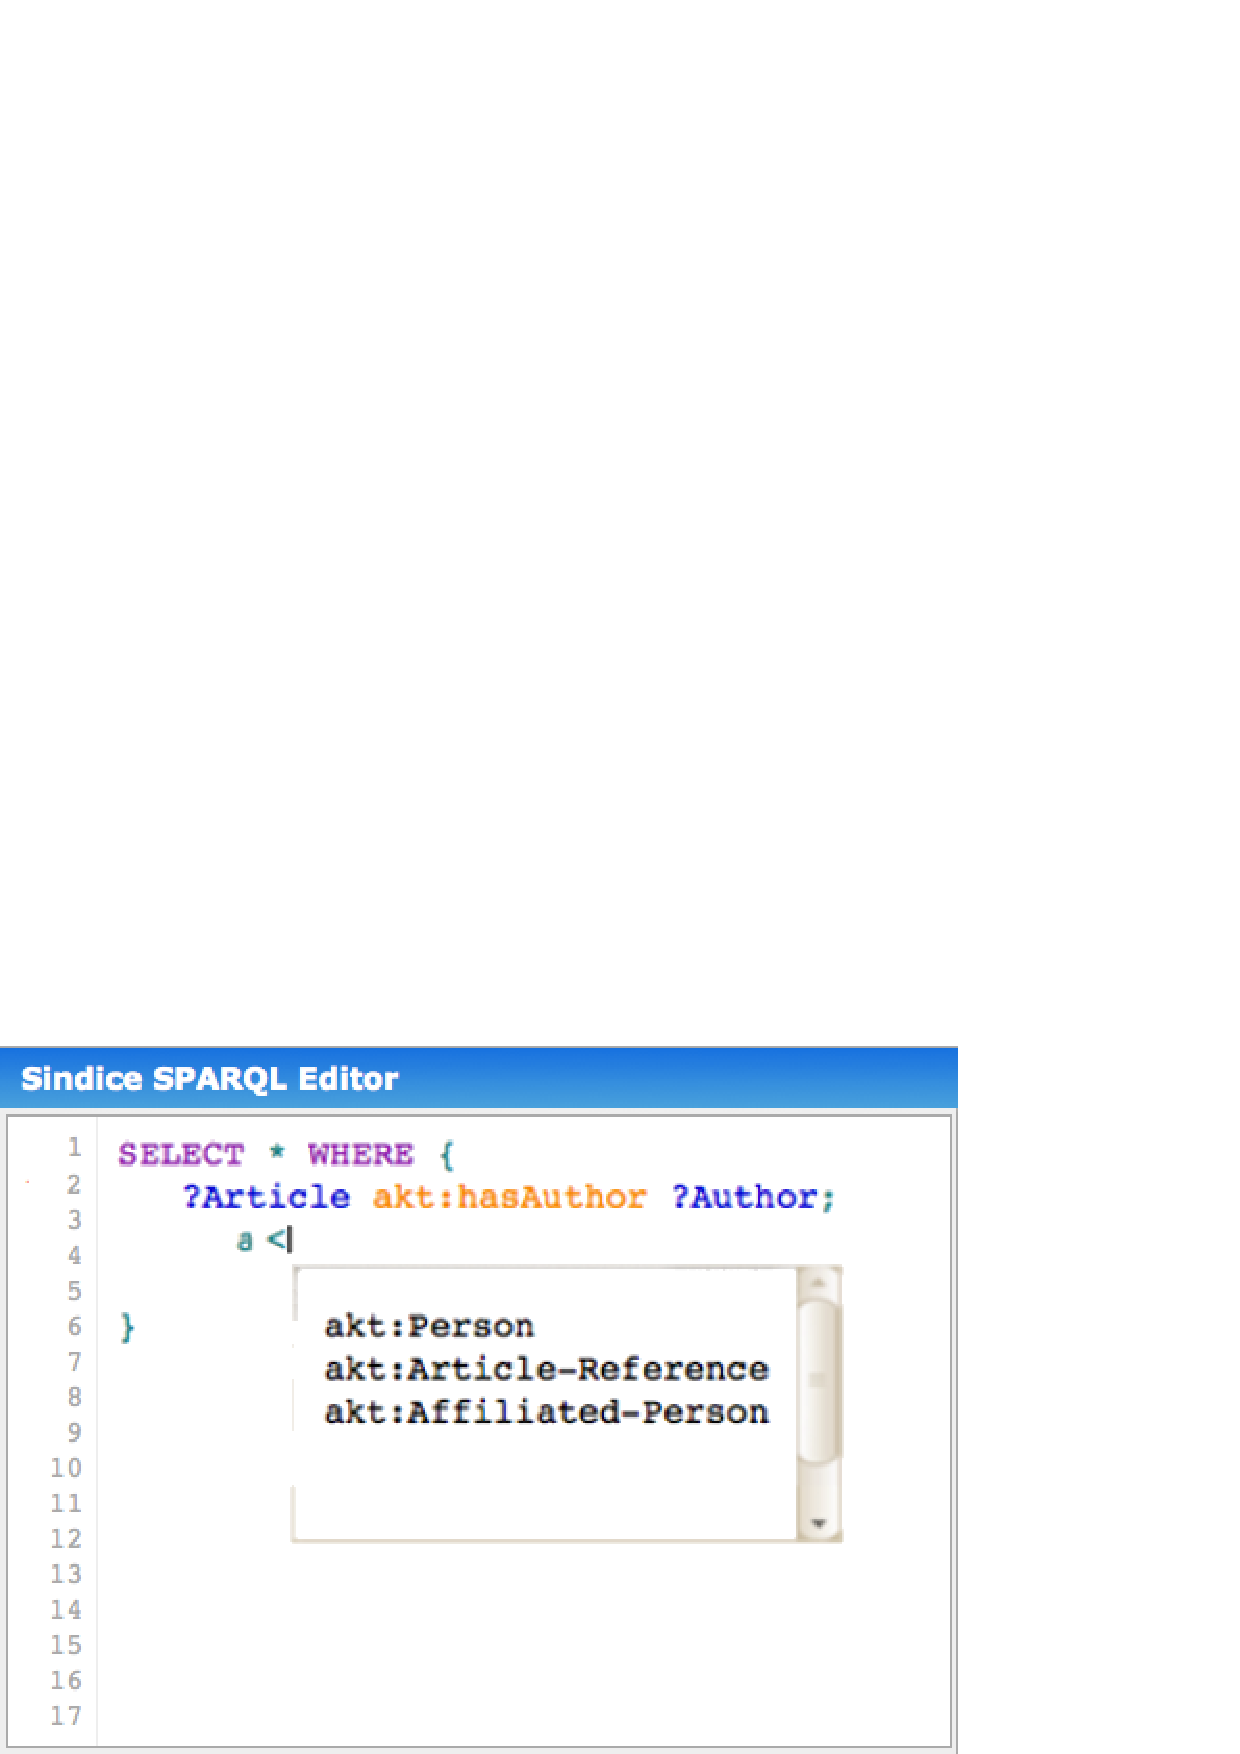
\includegraphics[scale=1]{exploiting/sparqled/figures/sparql/demo1.png}
		}
		\caption{Class}
		\label{fig:rkb-recommendations-types}
	\end{subfigure}
	\begin{subfigure}[t]{.475\textwidth}
		\resizebox{\textwidth}{!}{
			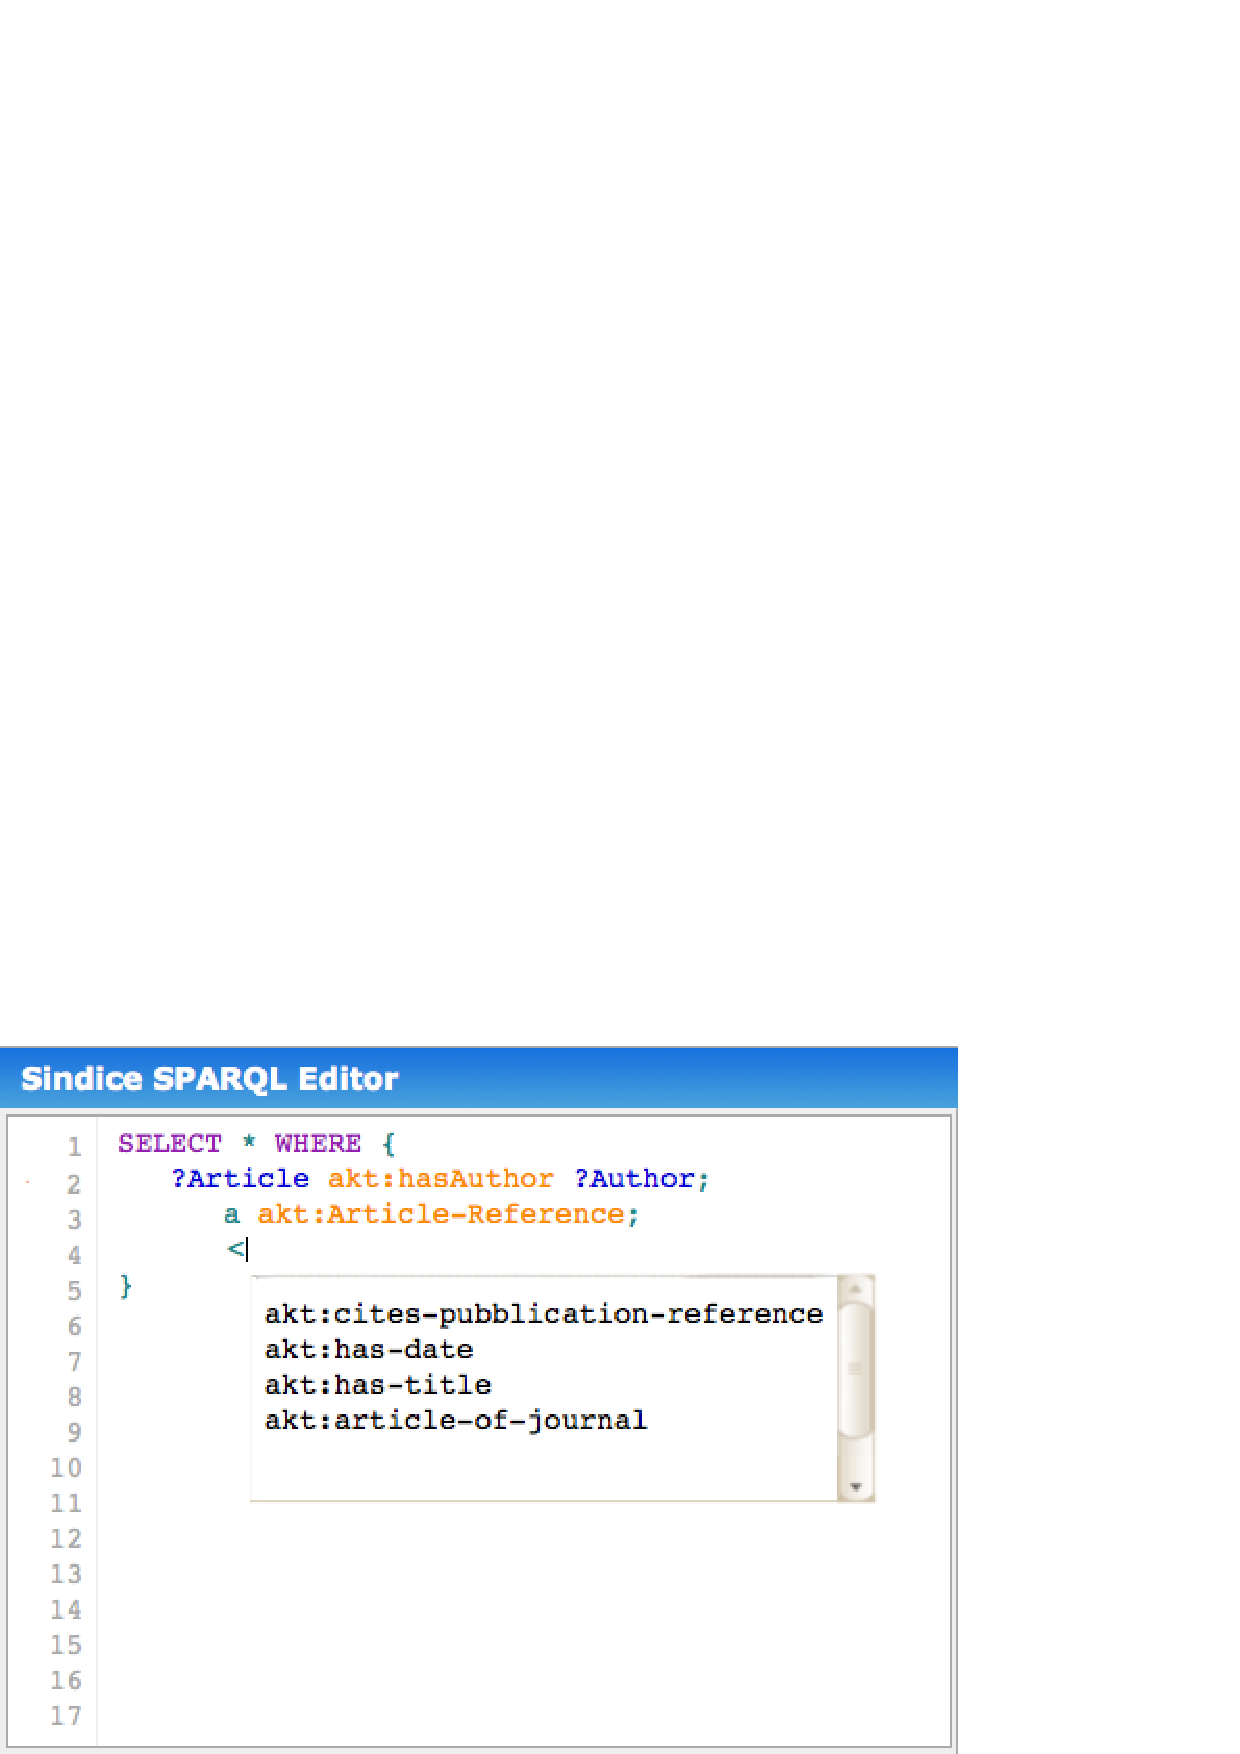
\includegraphics[scale=1]{exploiting/sparqled/figures/sparql/demo2.png}
		}
		\caption{Predicate}
		\label{fig:rkb-recommendations-predicates}
	\end{subfigure}
	\qquad
	\begin{subfigure}[b]{.475\textwidth}
		\resizebox{\textwidth}{!}{
			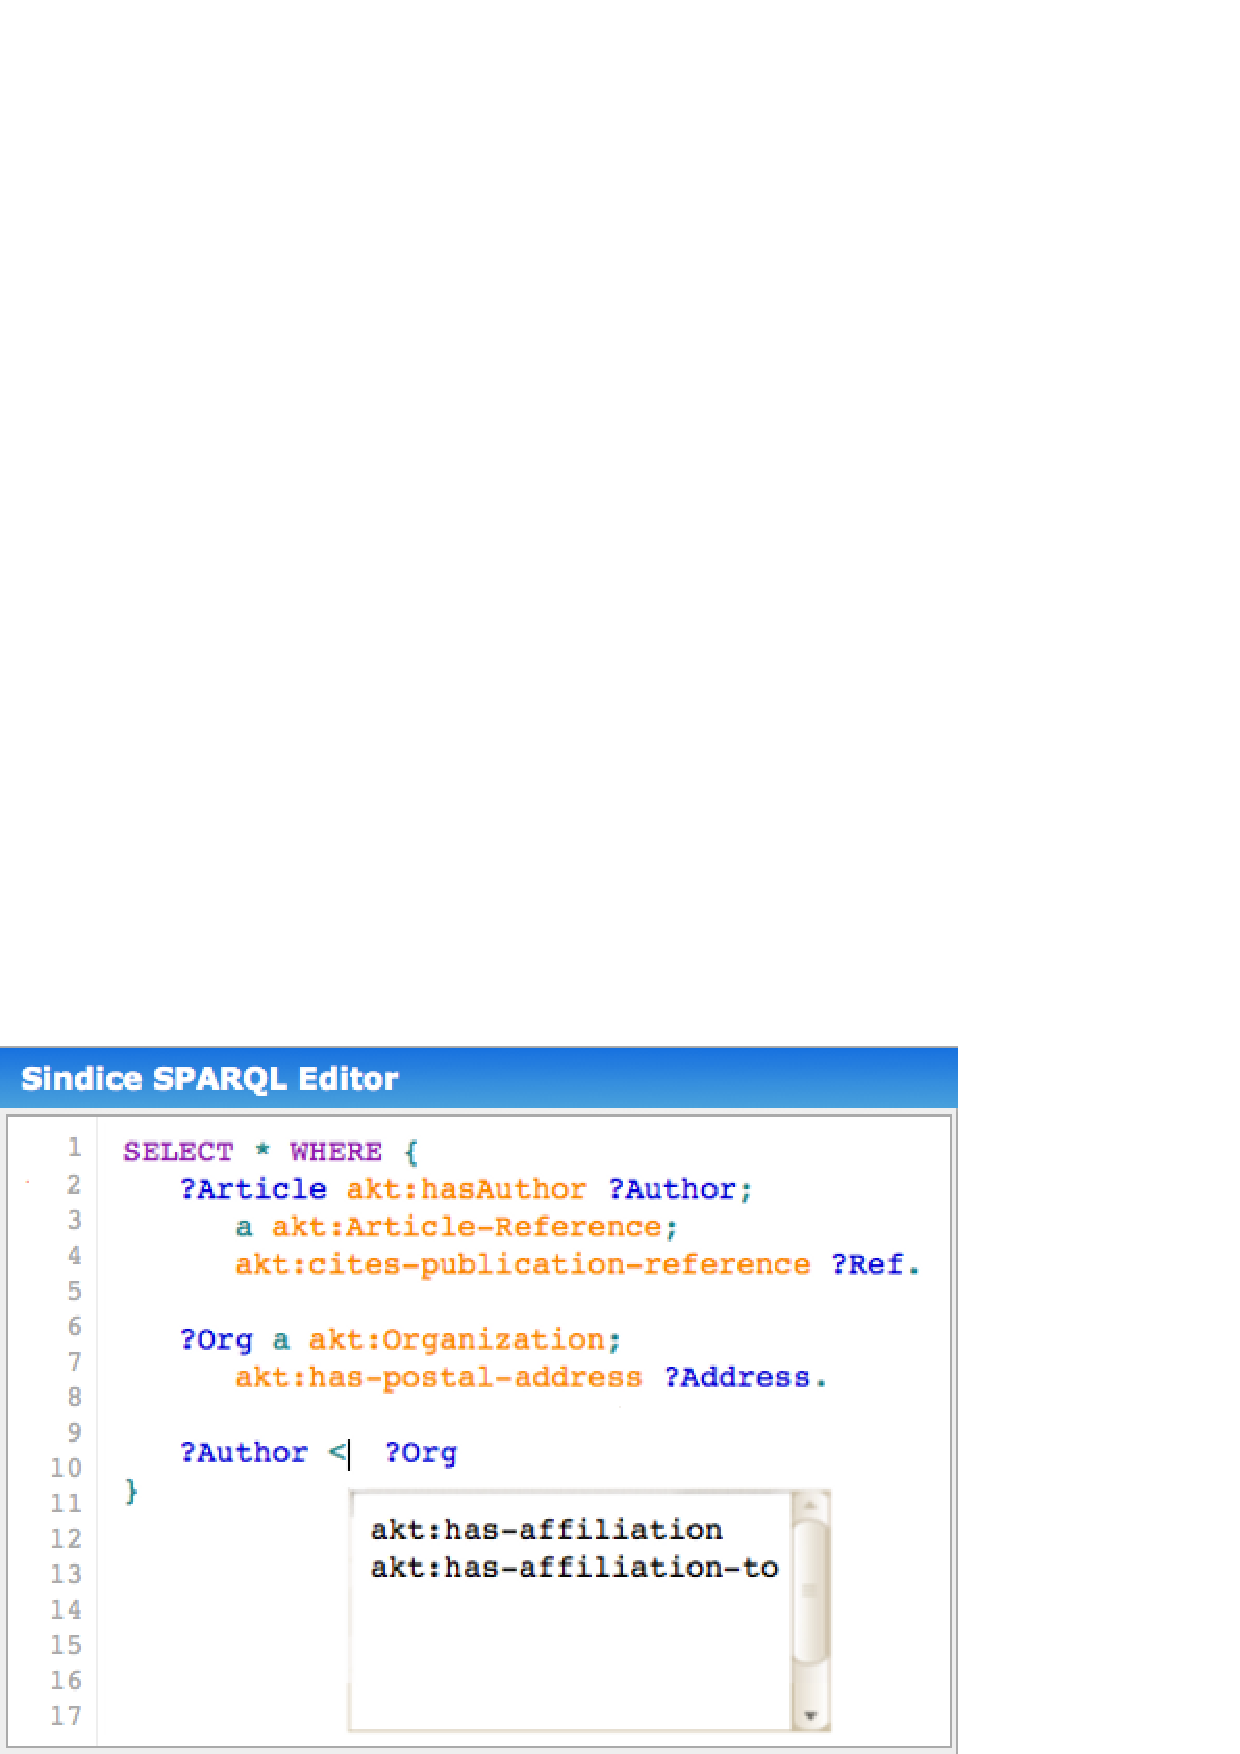
\includegraphics[scale=1]{exploiting/sparqled/figures/sparql/demo3.png}
		}
		\caption{Relationships}
		\label{fig:rkb-recommendations-relations}
	\end{subfigure}
	\begin{subfigure}[b]{.475\textwidth}
		\resizebox{\textwidth}{!}{
			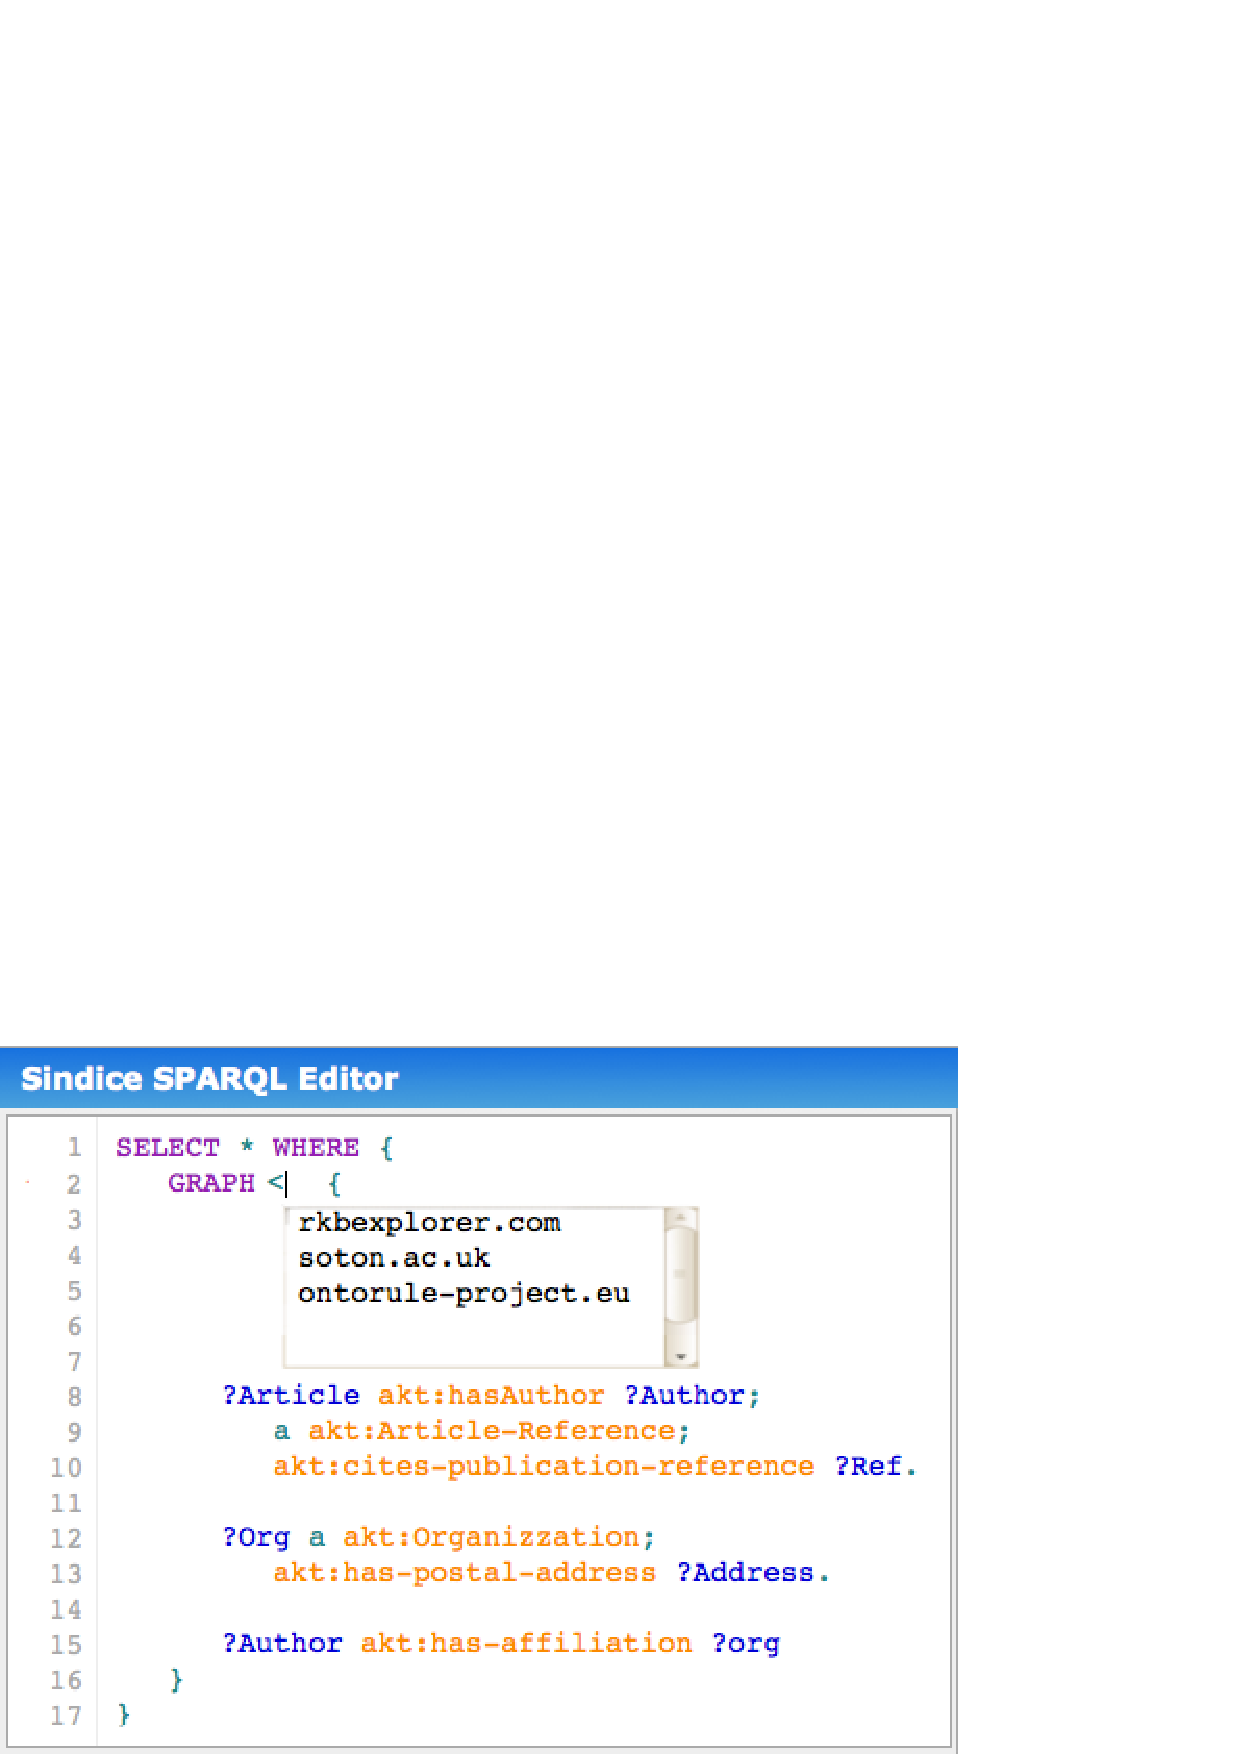
\includegraphics[scale=1]{exploiting/sparqled/figures/sparql/demo4.png}
		}
		\caption{Named Graphs}
    	\label{fig:rkb-recommendations-graph}
	\end{subfigure}
	\caption{Overview of the possible recommendations for the \url{http://www.rkbexplorer.com} dataset depending on the Point of Focus. The Point of Focus is displayed by the green angle bracket $<$.}
  \label{fig:rkb-recommendations}
\end{figure}

\subsection{SPARQL Graph Pattern}

In this section, we introduce the main concepts of SPARQL that are used later in the description of our recommendation engine. SPARQL is the standard query language for RDF data and is based around graph pattern matching. Triple Pattern (TP)~\cite{PrudS08} is the building block in SPARQL:

\begin{definition}[Triple Pattern] A triple pattern is a tuple $t \in (\mathcal{L}^{V^E} \cup Var) \times (\mathcal{L}^A \cup Var) \times (\mathcal{L}^V \cup Var)$ where $\mathcal{L}^{V^E}$ is the set of the entity node labels and $Var$ is an infinite set of variables.
\label{def:triple-pattern}
\end{definition}
The components of a triple pattern $t$ are denoted $subject(t)$, $predicate(t)$ and $object(t)$, respectively.

Triple patterns can be combined into a Basic Graph Pattern (BGP) \cite{PrudS08}. More complex graph patterns can be formed by combining BGPs in various ways~\cite{PrudS08}:\emph{Group Graph Pattern}, \emph{Optional Graph Pattern}, \emph{Alternative Graph Pattern} and \emph{Patterns on Named Graphs}.

A SPARQL query can be translated into an Abstract Syntax Tree (AST). The AST is a tree structure composed of all the logical operators of the query and where leaf nodes are triple patterns to be evaluated. Such an AST is the data structure used by the system to translate the current user needs into possible recommendations. In our implementation, the AST can contain an incomplete TP and a special symbol `$<$' to indicate the POF.

\subsection{From Data Graph to Data Graph Summary}

In order to suggest the possible structural elements to the user with respect to the current state of his query, we need to translate the AST of the query into another AST compatible with the data graph summary. This new AST is then evaluated on the data graph summary and the possible structural elements are retrieved and presented to the user. The AST translation is performed in three steps: 
\begin{inparaenum}
\item transformation of the POF symbol `$<$' into a variable to project as the query solution; 
\item removal of content elements from the AST; and
\item mapping of triple patterns into \emph{summary patterns}.
\end{inparaenum}
Figure~\ref{fig:entity-gs-sparql} depicts a translation of a data graph query (Figure~\ref{fig:entity-sparql}) to a data graph summary query (Figure~\ref{fig:gs-sparql}).

\begin{figure}

\newsavebox{\sparql}
\begin{lrbox}{\sparql}
\begin{minipage}{0.3\textwidth}
\centering
%% Because of syntax error in the query, and also becaus empty prefixes are not supported
\expandafter\def\csname PY@tok@err\endcsname{}
\begin{minted}[linenos,frame=lines,framesep=4mm]{sparql}
SELECT * WHERE {
 ?a a p:Article ;
    :title ?t .



 ?i a :Institute ;
    :employs ?p .



 ?p :name "Renaud" ;



    <


}
\end{minted}
\label{lst:sparql}
\end{minipage}
\end{lrbox}


\newsavebox{\sparqlSum}
\begin{lrbox}{\sparqlSum}
\begin{minipage}{0.4\textwidth}
\centering
\begin{minted}[linenos,frame=lines,framesep=4mm,]{sparql}
SELECT ?POF WHERE {
 ?a :label :Article .
 ?x :label :title ;
    :source ?a ;
    :target ?t .

 ?i :label :Institute .
 ?y :label :employs ;
    :source ?i ;
    :target ?p .

 ?z1 :label :name ;
     :source ?p ;
     :target ?_z1 .

 ?z2 :label ?POF ;
     :source ?p ;
     :target ?_z2 .
}
\end{minted}
\label{lst:gs-sparql}
\end{minipage}
\end{lrbox}

\begin{tabular}{crccr}
	\phantom{a}
	&
	\begin{subfigure}[t]{.275\textwidth}
		\centering
		\usebox{\sparql}
		\caption{SPARQL query over the data graph. The Point of Focus is depicted by the angle bracket $<$.}
		\label{fig:entity-sparql}
	\end{subfigure} 
	& \phantom{a} & \phantom{a} &
	\begin{subfigure}[t]{.55\textwidth}
		\centering
		\usebox{\sparqlSum}
		\caption{SPARQL query over the data graph summary. The Point Of Focus defines the solution set, i.e., the variable $?POF$ in the SELECT clause.}
		\label{fig:gs-sparql}
	\end{subfigure}
	\\
\end{tabular}
\caption{Mapping from a data graph query to a data graph summary query.}
\label{fig:entity-gs-sparql}
\end{figure}

\subsubsection{Summary Pattern}

Similar to Triple Patterns in SPARQL, Summary Patterns (SPs) are the building blocks to construct a data graph summary query.

\begin{definition}[Summary Pattern] 
A \emph{Summary Pattern} is a tuple $t \in  (\mathcal{L}^C \cup Var) \times (\mathcal{L}^A \cup Var) \times (\mathcal{L}^C \cup Var)$.
\label{def:summary-triple-pattern}
\end{definition}

With respect to our RDF data model of the data graph summary, such a summary pattern is translated into a SPARQL BGP. For example, given the SP \mbox{$<Institute, employs, ?p>$}, the corresponding SPARQL BGP is equal to the BGP in Figure~\ref{fig:gs-sparql} from the line 7 to line 10.

\subsubsection{Projection of POF}

The first step consists of defining the variable to project as the query solution. In the TP containing the POF, we transform the POF symbol into a variable $?POF$ and complete that TP with a wildcard variable if needed (we denote by wildcard variable a variable that is unique in the query). For example in Figures~\ref{fig:entity-sparql} and~\ref{fig:gs-sparql} at line 16, the POF symbol `$<$' is translated into the variable $?POF$, and the wildcard variable $?\_z2$ is added to complete the triple pattern.
The initial \emph{Query Form}~\cite{PrudS08} of the AST is replaced by a projection of the POF variable using the \emph{SELECT} form.

\subsubsection{Removal of content elements}

The second step consists in removing all content elements from the AST. A content element is an element that describes a specific aspect of an entity, thus it does not inform about its structure. We replace with a wildcard variable Literals and URIs that appear in a TP at a subject or object position, except if the TP is a \emph{Class Triple Pattern} (CTP). In that case, only the element at the subject position is replaced by a wildcard variable. For instance, the literal ``Renaud'' in Figure~\ref{fig:entity-sparql} is replaced by the variable $?\_z1$ in Figure~\ref{fig:gs-sparql}.

\begin{definition}[Class Triple Pattern] 
A \emph{Class Triple Pattern} is a triple pattern $t$ such as $predicate(t) \in \mathcal{L}^{A_c}$.
\label{def:class-triple-pattern}
\end{definition}

\subsubsection{Mapping}

The third step consists in mapping all triple patterns into summary patterns, according to the following two rules. If the triple pattern $<var_s, p, o>$ is a CTP, then it is replaced with a new triple pattern \mbox{$<var_s, label, o>$}. Otherwise, the triple pattern \mbox{$<var_s, p, var_o>$} is replaced with the following BGP:

\begin{enumerate}
    \item A new wildcard variable $var_x$, representing an edge node $x$, is created;
    \item A triple pattern $<var_x, source, var_s>$ is created to set the source of the edge;
    \item A triple pattern $<var_x, target, var_o>$ is created to set the target of the edge;
    \item A triple pattern $<var_x, label, p>$ is created to set the label of the edge.
\end{enumerate}

In the case where the triple pattern $<var_s, p, var_o>$ belongs to a \emph{Graph Graph Pattern}~\cite{PrudS08}, i.e., a group graph pattern associated to a named graph URI $g$ with the \emph{GRAPH} operator, then a triple pattern $<var_x, origin, g>$ is added to the previously defined BGP to set the named graph of the edge. However, if the named graph is the POF variable, the triple pattern $<var_x, origin, var_{POF}>$ is created instead in order to restrict each edge to be from the same dataset and to bind the dataset label to the POF variable.

Applying these mapping rules on the query of Figure~\ref{fig:entity-sparql}, the first TP \mbox{$<var_a, a, Article>$}, being a CTP, is translated into the SP \mbox{$<var_a, :label, Article>$}. The second TP \mbox{$<var_a, :title, var_t>$} is translated into the BGP from line 3 to line 5 of the query displayed in Figure~\ref{fig:gs-sparql}.

\subsection{Recommendation Scope}

In certain cases during the formulation of a query, the query may contain multiple BGPs, among which one does not return any result. The system will therefore no longer produce recommendations, as the evaluation of the data graph summary query will also not produce any results. However, this can be interpreted incorrectly by the user since he might believe that the dataset does not contain any other information. In order to minimise this issue, we introduce the notion of \emph{recommendation scope}.

The \emph{recommendation scope} helps to reduce the extent of the area that is relevant for the recommendation. Instead of taking into account the full SPARQL query, the recommendation engine will take only a relevant subset. The recommendation scope is defined recursively by including all the triple patterns with a path to the POF variable. A \emph{breadth-first search} algorithm on the query, starting on the POF node, is performed in order to find all the graph components that are connected to the POF. All the graph components that are not connected to the POF are removed. This prevents non-relevant (to the POF) triple patterns from limiting the recommendations. For example, in Figure~\ref{fig:entity-sparql}, the recommendation scope does not contain the first BGP since it is not connected to the POF variable, whether directly or indirectly. Another possible solution for this issue is to provide to the user an estimation of the cardinality of TPs or BGPs that can lead to an empty result set. This is possible given the cardinality information provided by the data graph summary. We are currently planning to investigate this solution for future works.


\subsection{Entity Authority}
\todo{move this to the applications part}

When working with the Web of Data, it is legitimate to wonder about the quality of the data. The quality not according to whether the data follows modelling standards or not, but rather to the information itself. Indeed, in an environment where data can be edited by anybody, it can happen that some statements about an entity, or relationships between two entities, can be erroneous. Therefore, there is a need to define the \emph{authority} of an entity in order to judge how much confidence one can put in the information about the entity that a dataset provides.\todo{Define the dataset set}

\begin{definition}[Entity Authority]
Let $v \in V$ an entity and $a_v : V \mapsto \mathcal{L}^D$ a function which assigns a dataset label to an entity, called the entity \emph{authority}. Statements about an entity are then said \emph{authoritative} if the dataset label given by $a_v$ and the label of the dataset where the statements are found are the same.
\end{definition}

For example, the authority of an entity is \emph{D1}, but a statement about that entity is found in a dataset labelled \emph{D2}; the validity of that statement should then be checked.


\bibliographystyle{alpha}{Default}
\bibliography{biblio,01-introduction/introduction,02-foundations/foundations,04-summary/bibliography,05-ranking/bibliography}

\cleardoubleoddpage
\printglossaries

\end{document}
